\chapter{Sensitivitätsanalyse}\label{ch:Sensitivity}
In diesem Kapitel wird das in Kapitel \ref{ch:ch2} hergeleitete nichtlineare Modell des Antriebsstrangs auf die Sensitivität verschiedener Parameter und Eingänge untersucht. Damit soll die Relevanz für eine Parameter- und Eingangsschätzung im folgenden Kapitel belegt und unterstrichen werden.
Eine mögliche Definition für eine Sensitivitätsanalyse ist die folgende: \emph{The study of how uncertainty in the output of a model (numerical or otherwise) can be apportioned to different sources of uncertainty in the model input} \cite{Saltelli.2004}.
Für die Analyse gibt es verschiedene Methoden. Dabei ist die OAT(one-at-a-time)-Methode wohl die einfachste. Hier wird pro Simulationsdurchlauf lediglich eine Eingangsgröße geändert während alle anderen auf den nominal Werten gehalten werden. Die Methode liefert aber nur eine sehr beschränkte Aussage über den gesamten Eingangsraum. Jedoch kann sie für die Abschätzung einer ersten Untergruppe an relevanten Eingängen hilfreich sein.    

 Die in der Literatur am häufigsten diskutierten Ansätze basieren auf partiellen Ableitungen der Art $\partial y_i/\partial x_i$ wobei $y$ ein beliebiger Ausgang und $x_i$ ein beliebiger Eingang des Systems ist. Ein Eingang kann hierbei auch ein variierender Parameter sein. Dieses Vorgehen wird vor allem bei relativ einfachen, mathematisch wohlbestimmten und stetigen Modellen verwendet. Der Vorteil dabei ist, dass die Sensitvitätsfunktionen sobald sie einmal berechnet sind leicht an Veränderungen anpassbar sind und auch für ähnliche Systeme verwendet werden können \cite{Karnavas.1993}. Jedoch werden die partiellen Ableitung immer in einem bestimmen Arbeitspunkt berechnet d.h. die Aussagen der Sensitvitätsfunktionen gelten für nichtlineare Systeme nur lokal um diesen den Arbeitspunkt. Des Weiteren ist es oft sehr schwer oder gar unmöglich die benötigten Ableitungen für komplexe Modelle zu berechnen.

Eine Alternative zur Berechnung der partiellen Ableitungen sind globale Methoden. Hierbei werden die Modelleingänge stochstisch varriert, woraus sich nach vielen Simulationen eine Strichprobe für die Modellausgänge ergibt. Dieses Methode der mehrfachen Simulation wird auch Monte-Carlo-Methode genannt. Wie der Name schon sagt ist der grundlegende Vorteil dabei, dass durch eine genügend große Stichprobe eine globale Aussage zur Sensitivität gegeben werden kann. Des weiteren erlaubt die Methode auch Aussagen über die verkoppelte Wirkung von Eingangsänderungen ohne spezielles Vorwissen über die Struktur des Modells. Der entscheidende Nachteil liegt je nach Stichprobengröße und Komplexität des Modells in der Rechenzeit.      

Aufgrund des stetigen Charakters von \eqref{eq:sys_nl23} werden für diese Arbeit die partiellen Ableitungen für die Sensitivitätsanalyse verwendet.
Hierfür wird zuerst ein idealer Schaltvorgang beschrieben um die Sensitivitätsfunktionen in verschieden Schaltphasen auswerten zu können. Des weiteren werden die Ergebnisse der Sensitivitätsanalyse für die Berechnung der Fisher-Informationsmatrix genutzt. Diese liefert eine Abschätzung für die erreichbare Genauigkeit einer Parameterschätzung.
   

\section{Anwendung der Parametersitivitätsanalyse}\label{sec:para_sens}
Wie einleitend erläutert werden die Sensitiviäten in dieser Arbeit mittels partiellen Differentialen berechnet. Nach \cite{Hearne.1985} ist für ein nichtlineares System erster Ordnung
\begin{equation}
\dot{\pmb{x}}_i = f_i(\pmb{x},\pmb{p},\pmb{u})\quad i=1,2,\,\dots\, ,n 
\end{equation}
mit dem Zustandsvektor $\pmb{x} = [x_1, x_2,\, \dots\, ,x_n]^T$, dem Parametervektor $\pmb{p} = [p_1, p_2,\, \dots\, ,p_m]^T$, dem Eingangsvektor $\pmb{u} = [u_1, u_2,\, \dots\, ,p_l]^T$ und der differenzierbaren Funktion $f_i$ die absolute Parametersensitivitätsfunktion definiert als
\begin{equation}\label{eq:abs_psens}
S_{ij} = \frac{\partial x_i}{\partial p_j} \quad i=1,2,\,\dots\, ,n \quad j=1,2,\,\dots\, ,m.
\end{equation}
Die entsprechende normalisierte Parametersensitivitätsfunktion ist 
\begin{equation}
S_{\mathrm{N},ij} = \frac{\partial x_i}{\partial p_j}\, \frac{p_{j0}}{x_{i0}} = \frac{\partial x_{\mathrm{N},i}}{\partial p_{\mathrm{N},j}}
\end{equation}
mit den normalisierten Zuständen $x_{\mathrm{N},i}$ und Parametern $p_{\mathrm{N},j}$, dem Nominalwert $p_{j0}$ des Parametern $p_{j}$ und dem Nominalwert $x_{i0}$ des  Zustandes $x_{i}$, welcher definiert wird als
\begin{equation}
 x_{i0} = \mathrm{max}\left( \left|x_{i}(t)\right|\right),\quad t_\mathrm{Start}\leq t \leq t_\mathrm{End}
\end{equation}
wobei $t_\mathrm{Start}$ bis $t_\mathrm{End}$ das ausgewertet Zeitfenster ist.
Die normalisierte Parametersensitivitätsfunktion $S_{\mathrm{N},ij}$ kann interpretiert werden, als approximierte prozentuale Änderung des Zustandes $x_i$ für eine $1\%$-ige Änderung des Parameters $p_j$. Das Modell des Antriebsstrangs ist mit \eqref{eq:sys_linex} in der Form
\begin{equation}
\dot{\pmb{x}} = \pmb{f}(t,\pmb{x}(t,\pmb{p}),\pmb{p})+ \pmb{B}(\pmb{p})\pmb{u}(t) 
\end{equation} 
gegeben. Wendet man \eqref{eq:abs_psens} auf diese Gleichung an erhält man
\begin{equation}\label{eq:Sens_eq1}
\partial\dot{\pmb{x}}/\partial p_j = \partial/\partial p_j\left(\pmb{f}(t,\pmb{x}(t,\pmb{p}),\pmb{p})+ \pmb{B}(\pmb{p})\pmb{u}(t)\right)
\end{equation}
und unter Berücksichtigung der Kettenregel
\begin{equation}\label{eq:Sens_eq}
\frac{\partial}{\partial p_j}\frac{\mathrm{d} \pmb{x}}{\mathrm{d} t} = \dot{\pmb{S}}_j= \frac{\partial\pmb{f}(t,\pmb{x}(t,\pmb{p}),\pmb{p})}{\partial \pmb{x}}\,\pmb{S}_j+\frac{\partial\pmb{f}(t,\pmb{x}(t,\pmb{p}),\pmb{p})}{\partial \pmb{p}}+\frac{\partial \pmb{B}(\pmb{p})}{\partial \pmb{p}}\,\pmb{u}(t).
\end{equation}
Die Gleichung \eqref{eq:Sens_eq1} kann auch als implizite Berechnung der Sensitivität der zeitlichen Ableitung von $\pmb{x}$ angesehen werden. Da für die Bewertung des Gangwechsels vor allem die Drehzahlbeschleunigungen betrachtet werden, wird im Folgenden auch der zeitliche Verlauf von $\dot{\pmb{S}}_j$ interpretiert. Dafür werden die Parametersensitivitätsfunktion anhand \eqref{eq:sys_nl23} für $m_\mathrm{veh}$, $k_\mathrm{ss}$, $d_\mathrm{ss}$, $\mu_{38}$ und $\zeta$ gebildet und für den in \ref{sec:Gangwechsel} definierten Schaltvorgang berechnet. Dabei ist der erste Term in \eqref{eq:Sens_eq} für alle Fälle gleich und kann daher pauschal für alle Parameter angegeben werden zu
\begin{equation}
\begin{split}
\pmb{J}_\mathrm{p}(t,\pmb{x}(t,\pmb{p}),\pmb{p})) &= \frac{\partial\pmb{f}(t,\pmb{x}(t,\pmb{p}),\pmb{p})}{\partial \pmb{x}}\\
 &= \begin{bmatrix} 0 & -0,799\,d_\mathrm{ss} & -1,97\,k_\mathrm{ss} & 1,97\,d_\mathrm{ss} \\  0 & -0,248\,d_\mathrm{ss} & -0,612\,k_\mathrm{ss} & 0,612\,d_\mathrm{ss} \\0 & 0,405 & 0 & -1,0 \\ 0 & \frac{42,6\,d_\mathrm{ss}}{5.69\,m_\mathrm{veh} + 337} & \frac{105\,k_\mathrm{ss}}{569\,m_\mathrm{veh}+337} & -\frac{1052\,d_\mathrm{ss} + 14,7\,\omega_\mathrm{C} + 558\,\partial f_{Roll}/\partial \omega_\mathrm{C}\,m_\mathrm{veh}\,\cos(\zeta)}{56,9\,m_\mathrm{veh} + 3370}\end{bmatrix}
\end{split}
\end{equation}

\subsection{Sensitivität des Zustandes $\pmb{x}$ von $k_\mathrm{ss}$}
Die Sensitivität von \eqref{eq:sys_nl23} zum Parameter $k_\mathrm{ss}$ ergibt sich mit \eqref{eq:Sens_eq} zu 
\begin{align}
\dot{\pmb{S}}_{k_\mathrm{ss}} = \left. \pmb{J}_\mathrm{p}(t,\pmb{x}(t,\pmb{p}),\pmb{p}))\right|_{\pmb{p}=\pmb{p}_0} \pmb{S}_{k_\mathrm{ss}} 
+ \begin{bmatrix} -1,97\,\phi \\ -0,612\,\phi \\ 0 \\ \frac{105\,\phi}{5,69\,m_\mathrm{veh} + 337} \end{bmatrix}.
\end{align}
In Abbildung \ref{fig:Sens_k} sind die Sensitivitäten der Zustände und deren Ableitungen zu $k_\mathrm{ss}$ abgebildet. Für $t<6\,s$ sind die Sensitivitäten alle bis auf $\frac{\partial \phi_\mathrm{N}}{\partial k_\mathrm{ss,N}}$ gleich Null, da hier $a_\mathrm{C}$ und somit $\phi$ konstant sind hat $k_\mathrm{ss}$ keine Auswirkung auf die Zustände und deren Ableitungen. Lediglich auf $\phi$ hat $k_\mathrm{ss}$ bei gleichbleibender Beschleunigung einen Einfluss. Dieser direkte Zusammenhang ist in \eqref{eq:Tout} leicht ersichtlich. Auch im weiteren Verlauf hat $k_\mathrm{ss}$ nur auf $\phi$ einen signifikanten Einfluss. Dieser Einfluss hängt maßgeblich vom Ausgangsmoment $T_\mathrm{out}$ des Getriebes ab. Damit lässt sich auch die geringere Sensitivität $\frac{\partial \phi_\mathrm{N}}{\partial k_\mathrm{ss,N}}$ nach dem Schaltvorgang erklären, da hier Aufgrund der niedrigeren Getriebeübersetzung $T_\mathrm{out}$ kleiner ist. Die relativ großen Schwingungen in allen Größen von $\dot{\pmb{S}}_{k_\mathrm{ss}}$ für $t>7\,s$ lassen sich auf das abrupte schließen von $B_{05}$ zurück führen. Dieses führt, wie in Abbildung \ref{fig:Gang23_Tandw} zu sehen, zu einem schnellen Abfallen von $T_\mathrm{K05}$ was zu Schwingungen im gesamten Antriebsstrang führt. Die Art der Schwingungen wiederum hängt maßgeblich von $k_\mathrm{ss}$ und $d_\mathrm{ss}$ ab. 

\begin{figure}
\centering
\newlength\kheight 
\setlength\kheight{8cm}
\newlength\kwidth 
\setlength\kwidth{13cm}
% This file was created by matlab2tikz.
%
%The latest updates can be retrieved from
%  http://www.mathworks.com/matlabcentral/fileexchange/22022-matlab2tikz-matlab2tikz
%where you can also make suggestions and rate matlab2tikz.
%
\definecolor{mycolor1}{rgb}{0.00000,0.44700,0.74100}%
\definecolor{mycolor2}{rgb}{0.85000,0.32500,0.09800}%
%
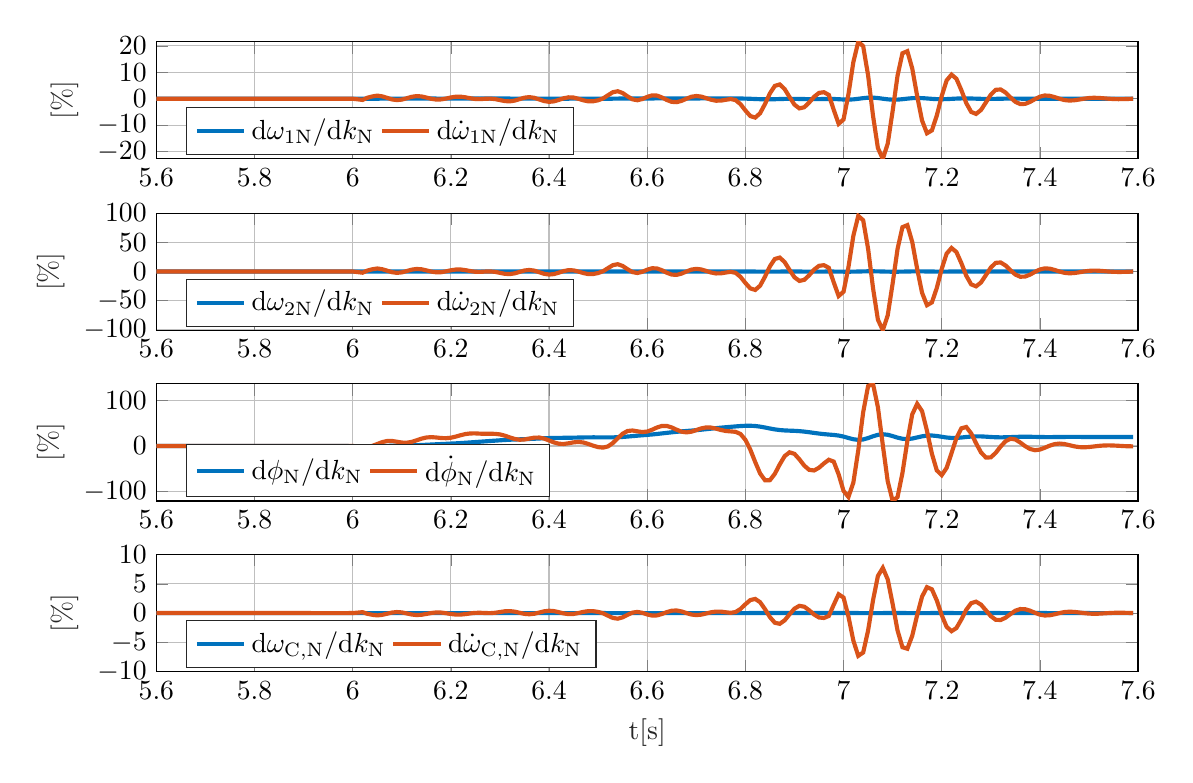
\begin{tikzpicture}

\begin{axis}[%
width=0.959\kwidth,
height=0.186\kheight,
at={(0\kwidth,0.814\kheight)},
scale only axis,
xmin=5.6,
xmax=7.6,
ymin=-22.7500670368041,
ymax=21.5401097966438,
ylabel style={font=\color{white!15!black}},
ylabel={[$\%$]},
axis background/.style={fill=white},
xmajorgrids,
ymajorgrids,
legend style={at={(0.03,0.03)}, anchor=south west, legend columns=2, legend cell align=left, align=left, draw=white!15!black}
]
\addplot [color=mycolor1, line width=1.5pt]
  table[row sep=crcr]{%
5.59	0\\
5.6	-4.49285731817047e-08\\
5.61	-9.0182236203473e-08\\
5.62	-1.35755506045401e-07\\
5.63	-1.81648844579986e-07\\
5.64	-2.27859338368798e-07\\
5.65	-2.74390390710852e-07\\
5.66	-3.21240905913487e-07\\
5.67	-3.68414302775877e-07\\
5.68	-4.15907946383393e-07\\
5.69	-4.6372313801538e-07\\
5.7	-5.11855682277668e-07\\
5.71	-5.60170002677743e-07\\
5.72	-6.08242717310906e-07\\
5.73	-6.55953557726372e-07\\
5.74	-7.0383231462743e-07\\
5.75	-7.52861200946703e-07\\
5.76	-8.03780707534743e-07\\
5.77	-8.56488578576185e-07\\
5.78	-9.09962691935074e-07\\
5.79	-9.62793383814237e-07\\
5.8	-1.0139520187904e-06\\
5.81	-1.06339842328936e-06\\
5.82	-1.11204899182843e-06\\
5.83	-1.16131727293037e-06\\
5.84	-1.21231202693291e-06\\
5.85	-1.26534790799404e-06\\
5.86	-1.31979069126152e-06\\
5.87	-1.37450342532066e-06\\
5.88	-1.42833300027756e-06\\
5.89	-1.48072418515284e-06\\
5.9	-1.53168427033676e-06\\
5.91	-1.58179214058973e-06\\
5.92	-1.62845965099866e-06\\
5.93	-1.56522926141458e-06\\
5.94	7.86491696664802e-07\\
5.95	1.39206549739558e-05\\
5.96	5.01428663124975e-05\\
5.97	0.000110704090482123\\
5.98	0.000177548768865427\\
5.99	0.000213559976593982\\
6	0.00019197727952979\\
6.01	-0.000575789828429831\\
6.02	-0.00583193112131338\\
6.03	-0.00616622548551546\\
6.04	0.00106342586256215\\
6.05	0.0134269423271765\\
6.06	0.0257976162647416\\
6.07	0.0331032645422768\\
6.08	0.0333170431996843\\
6.09	0.0284111866537024\\
6.1	0.023056148971602\\
6.11	0.02197052804866\\
6.12	0.0272552868736864\\
6.13	0.0374413147133162\\
6.14	0.0484141893003784\\
6.15	0.0561472019741847\\
6.16	0.0584971487494807\\
6.17	0.0562878275622396\\
6.18	0.052757844373631\\
6.19	0.051533751214271\\
6.2	0.0546641861495967\\
6.21	0.0620313785069171\\
6.22	0.0711828766118329\\
6.23	0.0788510948450257\\
6.24	0.0827628112828794\\
6.25	0.0828885305015406\\
6.26	0.0812466841579481\\
6.27	0.0802701871064101\\
6.28	0.080472471439348\\
6.29	0.0800914687934231\\
6.3	0.0763777340029839\\
6.31	0.0680744035068319\\
6.32	0.0567998180213581\\
6.33	0.0465518933937479\\
6.34	0.0414112519846863\\
6.35	0.0430143792848508\\
6.36	0.0492173976676515\\
6.37	0.0551404263530058\\
6.38	0.0558402516709982\\
6.39	0.0491352088127779\\
6.4	0.0368712440917024\\
6.41	0.0238785528184215\\
6.42	0.0153391702455592\\
6.43	0.0139153814432432\\
6.44	0.0183850554010951\\
6.45	0.0244510925612156\\
6.46	0.0271079907249227\\
6.47	0.0234326780992135\\
6.48	0.0139954001379905\\
6.49	0.00237805246097969\\
6.5	-0.00680028687734984\\
6.51	-0.010009429718636\\
6.52	-0.00217800535438015\\
6.53	0.0199175221403047\\
6.54	0.0514352739437891\\
6.55	0.0810256299908656\\
6.56	0.0987538160516095\\
6.57	0.102035862564688\\
6.58	0.0965628922147981\\
6.59	0.0919178569815298\\
6.6	0.0951417061648193\\
6.61	0.106961127153168\\
6.62	0.121812030658371\\
6.63	0.131794162683378\\
6.64	0.131772732627372\\
6.65	0.121804823321419\\
6.66	0.106939706052583\\
6.67	0.0943201694707133\\
6.68	0.0896057632666104\\
6.69	0.0941957208431531\\
6.7	0.104906191655173\\
6.71	0.115980068209572\\
6.72	0.122182455842682\\
6.73	0.121214338307657\\
6.74	0.114404063730929\\
6.75	0.105563136075522\\
6.76	0.0989395664112306\\
6.77	0.0962084713282017\\
6.78	0.0933856975393229\\
6.79	0.0793306498539286\\
6.8	0.0411672144157569\\
6.81	-0.023085795277597\\
6.82	-0.104040806633929\\
6.83	-0.17915432990108\\
6.84	-0.223606133944123\\
6.85	-0.223055702439988\\
6.86	-0.181571171161757\\
6.87	-0.119945194029362\\
6.88	-0.0657813888709059\\
6.89	-0.0406234585677051\\
6.9	-0.0508533828783691\\
6.91	-0.0865157386214335\\
6.92	-0.127866931189537\\
6.93	-0.155619511641276\\
6.94	-0.159522849548117\\
6.95	-0.141648058933989\\
6.96	-0.113484611421091\\
6.97	-0.089339781890511\\
6.98	-0.101635176328695\\
6.99	-0.18520710757413\\
7	-0.2933737119794\\
7.01	-0.332938669096935\\
7.02	-0.239151463303877\\
7.03	-0.0276550425561993\\
7.04	0.221483501637671\\
7.05	0.392436596288253\\
7.06	0.407741519236064\\
7.07	0.254756812746926\\
7.08	0.00649055887154314\\
7.09	-0.230609250955324\\
7.1	-0.359136633543221\\
7.11	-0.333899220858521\\
7.12	-0.176268627921581\\
7.13	0.0326105251798293\\
7.14	0.207967066885802\\
7.15	0.276699509972882\\
7.16	0.228144949412524\\
7.17	0.0994453279899925\\
7.18	-0.0500997152390329\\
7.19	-0.159026482071548\\
7.2	-0.190420569410605\\
7.21	-0.142641806469446\\
7.22	-0.0459799214076328\\
7.23	0.0524379616962432\\
7.24	0.116245450224691\\
7.25	0.12487204194049\\
7.26	0.0832638448423234\\
7.27	0.0183848633042403\\
7.28	-0.0410238884900316\\
7.29	-0.0747239538144627\\
7.3	-0.0739828130314376\\
7.31	-0.0442707874943451\\
7.32	-0.0031114156290711\\
7.33	0.0315743415753041\\
7.34	0.0482944526967737\\
7.35	0.0433575356976376\\
7.36	0.0232641338158752\\
7.37	-0.00039419337518848\\
7.38	-0.0190554633168686\\
7.39	-0.0269493335454347\\
7.4	-0.0229839070904867\\
7.41	-0.0109354150517522\\
7.42	0.00280591190659204\\
7.43	0.0129314328043949\\
7.44	0.0165112298919863\\
7.45	0.0134253501168107\\
7.46	0.00607487865216316\\
7.47	-0.00150795492927614\\
7.48	-0.00676911709002809\\
7.49	-0.00817730630814975\\
7.5	-0.006096369703258\\
7.51	-0.00245445656624667\\
7.52	0.00130658344471973\\
7.53	0.00384022695930728\\
7.54	0.00457434370240002\\
7.55	0.00376577926974232\\
7.56	0.002036557925399\\
7.57	0.000120482103991878\\
7.58	-0.00126005296963746\\
7.59	-0.00175430635055371\\
};
\addlegendentry{d$\omega_{1\mathrm{N}}/$d$k_\mathrm{N}$}

\addplot [color=mycolor2, line width=1.5pt]
  table[row sep=crcr]{%
5.59	-3.87054403766524e-06\\
5.6	-3.89976862393674e-06\\
5.61	-3.92669812076493e-06\\
5.62	-3.95540833167544e-06\\
5.63	-3.9819585912832e-06\\
5.64	-4.01054834720411e-06\\
5.65	-4.03721700217396e-06\\
5.66	-4.06603570894659e-06\\
5.67	-4.09287863497971e-06\\
5.68	-4.12170451722883e-06\\
5.69	-4.14837157764835e-06\\
5.7	-4.17691781563314e-06\\
5.71	-4.18111194808127e-06\\
5.72	-4.14977557921493e-06\\
5.73	-4.12297258337968e-06\\
5.74	-4.16408700063507e-06\\
5.75	-4.29240764125996e-06\\
5.76	-4.46885440202353e-06\\
5.77	-4.60462285504727e-06\\
5.78	-4.63157872839552e-06\\
5.79	-4.53442370687234e-06\\
5.8	-4.37290878048693e-06\\
5.81	-4.23809167605451e-06\\
5.82	-4.20865036381717e-06\\
5.83	-4.30252114317494e-06\\
5.84	-4.47562366681688e-06\\
5.85	-4.64606262700982e-06\\
5.86	-4.73869264689116e-06\\
5.87	-4.72442647083666e-06\\
5.88	-4.62043109415119e-06\\
5.89	-4.48780596490734e-06\\
5.9	-4.37353151883085e-06\\
5.91	-4.31738966061703e-06\\
5.92	-2.97280715181311e-06\\
5.93	2.57447147055263e-05\\
5.94	0.000471504128044984\\
5.95	0.00197789387706473\\
5.96	0.00431281869008232\\
5.97	0.00592630050494981\\
5.98	0.0051311384407245\\
5.99	0.00103723082527468\\
6	-0.00473085519023981\\
6.01	-0.223074080262117\\
6.02	-0.46040052133978\\
6.03	0.377142301873422\\
6.04	0.867291957393148\\
6.05	1.1739623581065\\
6.06	0.898200204467263\\
6.07	0.331112512426292\\
6.08	-0.261366908170851\\
6.09	-0.51878165524268\\
6.1	-0.33485772628973\\
6.11	0.178269919862509\\
6.12	0.714782793104749\\
6.13	0.987030206874243\\
6.14	0.866379281691512\\
6.15	0.447501562954867\\
6.16	-0.0301600322622921\\
6.17	-0.310958719519488\\
6.18	-0.26144169051644\\
6.19	0.0621641513141646\\
6.2	0.477373254857071\\
6.21	0.763259044915417\\
6.22	0.773455968695502\\
6.23	0.518340176672106\\
6.24	0.158177607779356\\
6.25	-0.106060066222544\\
6.26	-0.141895669258328\\
6.27	-0.0208341092151094\\
6.28	0.0366697024410895\\
6.29	-0.138506574740039\\
6.3	-0.520856228886737\\
6.31	-0.895159125667356\\
6.32	-0.998882016492137\\
6.33	-0.71161943724178\\
6.34	-0.144631643629965\\
6.35	0.398978669360867\\
6.36	0.605182512498232\\
6.37	0.341362542594335\\
6.38	-0.262704949569236\\
6.39	-0.879727971536764\\
6.4	-1.17525726349705\\
6.41	-0.992458238738256\\
6.42	-0.437025767572009\\
6.43	0.181167291222738\\
6.44	0.532918991731604\\
6.45	0.439122940936568\\
6.46	-0.0308393098045711\\
6.47	-0.605373620911636\\
6.48	-0.98001790711821\\
6.49	-0.960353568615616\\
6.5	-0.584008879477933\\
6.51	0.10480236020596\\
6.52	1.30309480963421\\
6.53	2.45848558041844\\
6.54	2.82823257893463\\
6.55	2.15164598811073\\
6.56	0.877319241648224\\
6.57	-0.225311402923428\\
6.58	-0.574020480071075\\
6.59	-0.119569208638378\\
6.6	0.6973544886126\\
6.61	1.26644946603151\\
6.62	1.18712120652299\\
6.63	0.475955333511289\\
6.64	-0.477983358638592\\
6.65	-1.18348842546119\\
6.66	-1.29983565621785\\
6.67	-0.806673273483268\\
6.68	0.0133219399601675\\
6.69	0.736763772786241\\
6.7	1.03159651189386\\
6.71	0.806396324649976\\
6.72	0.232073662821699\\
6.73	-0.379738975649946\\
6.74	-0.742412707258588\\
6.75	-0.724160317845759\\
6.76	-0.399570279877154\\
6.77	-0.120272268337033\\
6.78	-0.508725224272759\\
6.79	-2.04929473752854\\
6.8	-4.4275231707968\\
6.81	-6.53926346770711\\
6.82	-7.1357084411461\\
6.83	-5.49062115555497\\
6.84	-1.98347672261123\\
6.85	2.01771968199367\\
6.86	4.84921958733974\\
6.87	5.40154546903996\\
6.88	3.65080750907164\\
6.89	0.611314185638254\\
6.9	-2.22794727448271\\
6.91	-3.64529744610254\\
6.92	-3.2216478503455\\
6.93	-1.42556961088923\\
6.94	0.719911655601597\\
6.95	2.19892097341674\\
6.96	2.46080531763678\\
6.97	1.43577739117109\\
6.98	-4.18204450320167\\
6.99	-9.4869612502387\\
7	-7.83120535494804\\
7.01	1.70514297916307\\
7.02	13.8563344988911\\
7.03	21.5401097966438\\
7.04	19.8667670485337\\
7.05	8.84768393484158\\
7.06	-6.34955942454012\\
7.07	-18.6501150051682\\
7.08	-22.7500670368041\\
7.09	-16.9897421575615\\
7.1	-4.66882868724555\\
7.11	8.7020838422154\\
7.12	17.1795436956383\\
7.13	17.9616324275848\\
7.14	11.4008500388914\\
7.15	1.01109572497408\\
7.16	-8.2648972167819\\
7.17	-13.0565485506077\\
7.18	-11.971443005793\\
7.19	-6.36224634860297\\
7.2	0.991341966124954\\
7.21	6.91569201313507\\
7.22	9.11275938120339\\
7.23	7.53432434530711\\
7.24	3.25096570550131\\
7.25	-1.62837300639731\\
7.26	-4.97488279722277\\
7.27	-5.74438186911126\\
7.28	-4.26122309323467\\
7.29	-1.40293249055528\\
7.3	1.52976805292653\\
7.31	3.36057586578023\\
7.32	3.50182794997986\\
7.33	2.34783106267032\\
7.34	0.504270236729165\\
7.35	-1.17420225205264\\
7.36	-2.02004721130178\\
7.37	-1.95142163937466\\
7.38	-1.20681107637371\\
7.39	-0.143163862177329\\
7.4	0.7731389050074\\
7.41	1.22196284538184\\
7.42	1.09890477912903\\
7.43	0.617416427071011\\
7.44	-0.00311772494129782\\
7.45	-0.503667036058394\\
7.46	-0.692044816823741\\
7.47	-0.592975864732928\\
7.48	-0.31219014807466\\
7.49	0.0217746394279011\\
7.5	0.257689969753261\\
7.51	0.362916888144055\\
7.52	0.300574361202384\\
7.53	0.160289652491485\\
7.54	0.00242076031753737\\
7.55	-0.11735648542367\\
7.56	-0.172287858288196\\
7.57	-0.151399181885812\\
7.58	-0.0844824244832335\\
7.59	-0.0015663374162484\\
};
\addlegendentry{d$\dot{\omega}_{1\mathrm{N}}/$d$k_\mathrm{N}$}

\end{axis}

\begin{axis}[%
width=0.959\kwidth,
height=0.186\kheight,
at={(0\kwidth,0.542\kheight)},
scale only axis,
xmin=5.6,
xmax=7.6,
ymin=-100.476642933101,
ymax=100,
ylabel style={font=\color{white!15!black}},
ylabel={[$\%$]},
axis background/.style={fill=white},
xmajorgrids,
ymajorgrids,
legend style={at={(0.03,0.03)}, anchor=south west, legend columns=2, legend cell align=left, align=left, draw=white!15!black}
]
\addplot [color=mycolor1, line width=1.5pt]
  table[row sep=crcr]{%
5.59	0\\
5.6	-4.22295526829419e-08\\
5.61	-8.47646663339644e-08\\
5.62	-1.27600185378129e-07\\
5.63	-1.70736546837411e-07\\
5.64	-2.14171010554536e-07\\
5.65	-2.57906776155305e-07\\
5.66	-3.01942813179538e-07\\
5.67	-3.46282334932415e-07\\
5.68	-3.90922864816651e-07\\
5.69	-4.35865626449759e-07\\
5.7	-4.81106676219255e-07\\
5.71	-5.26518582603997e-07\\
5.72	-5.71703396875923e-07\\
5.73	-6.16548076191402e-07\\
5.74	-6.61550584850511e-07\\
5.75	-7.07634129433827e-07\\
5.76	-7.55494718166172e-07\\
5.77	-8.0503623847794e-07\\
5.78	-8.55297970530584e-07\\
5.79	-9.04954934112653e-07\\
5.8	-9.53040287970193e-07\\
5.81	-9.99516270486265e-07\\
5.82	-1.0452442253491e-06\\
5.83	-1.09155278424852e-06\\
5.84	-1.13948410005105e-06\\
5.85	-1.18933392543629e-06\\
5.86	-1.24050613533333e-06\\
5.87	-1.29193207964528e-06\\
5.88	-1.34252791943696e-06\\
5.89	-1.39177177907408e-06\\
5.9	-1.43967050966989e-06\\
5.91	-1.4867682213706e-06\\
5.92	-1.53063224778632e-06\\
5.93	-1.47120033581964e-06\\
5.94	7.39244281963581e-07\\
5.95	1.30843911610764e-05\\
5.96	4.71306042604887e-05\\
5.97	0.000104053698292162\\
5.98	0.000166882776871455\\
5.99	0.000200730662060546\\
6	0.000180444515170943\\
6.01	-0.000541200059506482\\
6.02	-0.00548158606984968\\
6.03	-0.00579579816145032\\
6.04	0.000999542063506197\\
6.05	0.0126203376886405\\
6.06	0.0242478608350417\\
6.07	0.031114632590325\\
6.08	0.0313155687738095\\
6.09	0.0267044246448869\\
6.1	0.0216710833021264\\
6.11	0.0206506795262612\\
6.12	0.0256179639192395\\
6.13	0.0351920804957671\\
6.14	0.0455057751106912\\
6.15	0.0527742387396984\\
6.16	0.0549830160447146\\
6.17	0.0529064161876144\\
6.18	0.0495884917644356\\
6.19	0.0484379319756939\\
6.2	0.0513803094401561\\
6.21	0.0583049281890811\\
6.22	0.0669066635825192\\
6.23	0.0741142243457826\\
6.24	0.0777909498528345\\
6.25	0.0779091166223356\\
6.26	0.076365901803838\\
6.27	0.0754480664314124\\
6.28	0.0756381991904459\\
6.29	0.0752800847648272\\
6.3	0.0717894478664898\\
6.31	0.0639849281271901\\
6.32	0.0533876473337871\\
6.33	0.0437553521106084\\
6.34	0.0389235278272236\\
6.35	0.0404303504465919\\
6.36	0.0462607313541007\\
6.37	0.051827942402254\\
6.38	0.0524857267073806\\
6.39	0.0461834789074762\\
6.4	0.0346562544377532\\
6.41	0.0224440808210611\\
6.42	0.0144176896117919\\
6.43	0.0130794338021522\\
6.44	0.0172805985315195\\
6.45	0.0229822270180795\\
6.46	0.0254795157757778\\
6.47	0.022024992377189\\
6.48	0.0131546443430111\\
6.49	0.00223519230247005\\
6.5	-0.00639177105382274\\
6.51	-0.00940812917139721\\
6.52	-0.00204716659253634\\
6.53	0.0187210033369293\\
6.54	0.0483453706363041\\
6.55	0.0761581278947226\\
6.56	0.0928213181414096\\
6.57	0.0959061997878874\\
6.58	0.0907620102834669\\
6.59	0.0863960190017879\\
6.6	0.0894262008242203\\
6.61	0.100535586744\\
6.62	0.114494343686723\\
6.63	0.123876813197649\\
6.64	0.123856670933719\\
6.65	0.114487569173292\\
6.66	0.1005154528713\\
6.67	0.0886540167728783\\
6.68	0.084222822098496\\
6.69	0.0885370444118961\\
6.7	0.0986040991945651\\
6.71	0.109012728214327\\
6.72	0.114842516062976\\
6.73	0.113932556812445\\
6.74	0.107531399729083\\
6.75	0.0992215783244107\\
6.76	0.0929959101638507\\
6.77	0.0904288819694396\\
6.78	0.0877756828430352\\
6.79	0.074564972914107\\
6.8	0.0386941527434477\\
6.81	-0.0216989480610361\\
6.82	-0.0977907013021885\\
6.83	-0.168391885541766\\
6.84	-0.210173309852698\\
6.85	-0.209655944725812\\
6.86	-0.170663538184216\\
6.87	-0.112739654809918\\
6.88	-0.0618296639599417\\
6.89	-0.0381830608685475\\
6.9	-0.0477984368998462\\
6.91	-0.0813184268858873\\
6.92	-0.120185504853245\\
6.93	-0.146270887773082\\
6.94	-0.149939738096586\\
6.95	-0.133138750306626\\
6.96	-0.106667182309348\\
6.97	-0.0839728194856911\\
6.98	-0.0955295853184234\\
6.99	-0.174081050534516\\
7	-0.275749698833615\\
7.01	-0.312937847283724\\
7.02	-0.224784776531742\\
7.03	-0.0259937048782356\\
7.04	0.208178192705995\\
7.05	0.368861521810559\\
7.06	0.383247023627517\\
7.07	0.239452658606502\\
7.08	0.00610064954178716\\
7.09	-0.216755723670829\\
7.1	-0.33756200541379\\
7.11	-0.313840694634341\\
7.12	-0.165679537793161\\
7.13	0.0306514947943467\\
7.14	0.195473739662517\\
7.15	0.260077178096544\\
7.16	0.214439464312478\\
7.17	0.0934712911736295\\
7.18	-0.0470900447049658\\
7.19	-0.149473189965027\\
7.2	-0.178981321770957\\
7.21	-0.134072798574024\\
7.22	-0.0432177403126422\\
7.23	0.0492878272144888\\
7.24	0.109262171320064\\
7.25	0.117370532491614\\
7.26	0.078261889547658\\
7.27	0.0172804213628942\\
7.28	-0.0385594334638998\\
7.29	-0.0702350148569542\\
7.3	-0.0695383949251605\\
7.31	-0.0416112774232881\\
7.32	-0.00292449683459283\\
7.33	0.0296775626939881\\
7.34	0.0453932368061762\\
7.35	0.0407528980345093\\
7.36	0.0218665791289585\\
7.37	-0.000370507398350062\\
7.38	-0.0179107281318964\\
7.39	-0.0253303851553376\\
7.4	-0.0216031761032139\\
7.41	-0.0102784801800652\\
7.42	0.0026373559748585\\
7.43	0.0121546006158116\\
7.44	0.0155193464221175\\
7.45	0.0126188462739844\\
7.46	0.00570994399612744\\
7.47	-0.00141736155392472\\
7.48	-0.00636246682588886\\
7.49	-0.00768606106682072\\
7.5	-0.00573013462434192\\
7.51	-0.00230700430268678\\
7.52	0.00122809653171723\\
7.53	0.00360953513131925\\
7.54	0.00429955109537992\\
7.55	0.00353956018143289\\
7.56	0.00191421934356445\\
7.57	0.000113249070202669\\
7.58	-0.00118435230693109\\
7.59	-0.00164891414891819\\
};
\addlegendentry{d$\omega_{2\mathrm{N}}/$d$k_\mathrm{N}$}

\addplot [color=mycolor2, line width=1.5pt]
  table[row sep=crcr]{%
5.59	-1.70944232765467e-05\\
5.6	-1.72234945516405e-05\\
5.61	-1.73424307637589e-05\\
5.62	-1.74692303745682e-05\\
5.63	-1.75864906989533e-05\\
5.64	-1.77127584171148e-05\\
5.65	-1.78305418796869e-05\\
5.66	-1.79578206197719e-05\\
5.67	-1.80763737650767e-05\\
5.68	-1.82036844471134e-05\\
5.69	-1.8321460811474e-05\\
5.7	-1.8447535931497e-05\\
5.71	-1.84660596608137e-05\\
5.72	-1.83276613358194e-05\\
5.73	-1.82092846993736e-05\\
5.74	-1.83908685430855e-05\\
5.75	-1.89576018155699e-05\\
5.76	-1.97368867722566e-05\\
5.77	-2.03365133934021e-05\\
5.78	-2.04555650697607e-05\\
5.79	-2.00264762922103e-05\\
5.8	-1.93131386890327e-05\\
5.81	-1.87177130260552e-05\\
5.82	-1.85876844388382e-05\\
5.83	-1.90022689676329e-05\\
5.84	-1.97667834926329e-05\\
5.85	-2.0519534151727e-05\\
5.86	-2.09286383880357e-05\\
5.87	-2.08656315869407e-05\\
5.88	-2.04063314016378e-05\\
5.89	-1.98205869893143e-05\\
5.9	-1.93158894825929e-05\\
5.91	-1.90679361783951e-05\\
5.92	-1.31295300914892e-05\\
5.93	0.000113702631696049\\
5.94	0.00208241812378527\\
5.95	0.00873545280179372\\
5.96	0.0190477479844969\\
5.97	0.026173759346439\\
5.98	0.0226618921208992\\
5.99	0.0045809742488163\\
6	-0.0208940240465296\\
6.01	-0.985216205027945\\
6.02	-2.03337857044682\\
6.03	1.66566508744785\\
6.04	3.83043197986014\\
6.05	5.18485490533044\\
6.06	3.96693957343941\\
6.07	1.46237255599758\\
6.08	-1.15433811532654\\
6.09	-2.29122134232604\\
6.1	-1.47891345301889\\
6.11	0.78733671662415\\
6.12	3.15686874070854\\
6.13	4.35926107381774\\
6.14	3.82640110863482\\
6.15	1.9764097697064\\
6.16	-0.133203070899294\\
6.17	-1.37336246867136\\
6.18	-1.15466839475023\\
6.19	0.274550629882474\\
6.2	2.10833937308782\\
6.21	3.37096617769736\\
6.22	3.41600132717715\\
6.23	2.28927153335917\\
6.24	0.698598161980518\\
6.25	-0.468418813275014\\
6.26	-0.626688284951475\\
6.27	-0.0920147333656238\\
6.28	0.161953307331681\\
6.29	-0.61172020423202\\
6.3	-2.30038378544882\\
6.31	-3.95350851900755\\
6.32	-4.41160509729567\\
6.33	-3.1428976444039\\
6.34	-0.638771832642413\\
6.35	1.76210633728838\\
6.36	2.67281441937155\\
6.37	1.5076422521082\\
6.38	-1.16024763232252\\
6.39	-3.88535616758242\\
6.4	-5.19057391030545\\
6.41	-4.38323420842693\\
6.42	-1.93014297188089\\
6.43	0.800133081010099\\
6.44	2.35365949286464\\
6.45	1.93940522763483\\
6.46	-0.136203129183362\\
6.47	-2.67365845784349\\
6.48	-4.32829095238589\\
6.49	-4.24144256134369\\
6.5	-2.57930016461671\\
6.51	0.462864100924658\\
6.52	5.75517389393925\\
6.53	10.8580065904975\\
6.54	12.4910100047462\\
6.55	9.50283642312279\\
6.56	3.87471790913012\\
6.57	-0.995097436138308\\
6.58	-2.53518597193935\\
6.59	-0.528082517854513\\
6.6	3.07989588939548\\
6.61	5.59332816845788\\
6.62	5.24297152149728\\
6.63	2.10207706289172\\
6.64	-2.11103392250255\\
6.65	-5.22692718874833\\
6.66	-5.74077970364803\\
6.67	-3.56270697278974\\
6.68	0.058836916937084\\
6.69	3.25394867648251\\
6.7	4.55609006377439\\
6.71	3.56148381643619\\
6.72	1.02496324585706\\
6.73	-1.67713340810983\\
6.74	-3.27889743689728\\
6.75	-3.19828497932774\\
6.76	-1.76471921040714\\
6.77	-0.531187611047925\\
6.78	-2.2468066853441\\
6.79	-9.05079775256185\\
6.8	-19.554345224148\\
6.81	-28.8809364573449\\
6.82	-31.5151611622007\\
6.83	-24.2495628885463\\
6.84	-8.76010967798559\\
6.85	8.91134517092995\\
6.86	21.4167854623508\\
6.87	23.8561563138093\\
6.88	16.1239473234539\\
6.89	2.69989521573462\\
6.9	-9.8398243139165\\
6.91	-16.0996118949656\\
6.92	-14.2285453573257\\
6.93	-6.29608908571041\\
6.94	3.17952058102683\\
6.95	9.71162841527731\\
6.96	10.86825180902\\
6.97	6.34117218339328\\
6.98	-18.4701782020579\\
6.99	-41.899569637238\\
7	-34.5868529930907\\
7.01	7.53083680984686\\
7.02	61.1970932461154\\
7.03	95.1328150935065\\
7.04	87.7424253625855\\
7.05	39.0761740643591\\
7.06	-28.0431004466899\\
7.07	-82.369029638639\\
7.08	-100.476642933101\\
7.09	-75.0359220273563\\
7.1	-20.6200813459265\\
7.11	38.4331250353541\\
7.12	75.874188628445\\
7.13	79.3283169233048\\
7.14	50.352341232153\\
7.15	4.46554746256554\\
7.16	-36.5022716278567\\
7.17	-57.6648044392924\\
7.18	-52.8723894457592\\
7.19	-28.0991327887887\\
7.2	4.37830414274356\\
7.21	30.5434492089601\\
7.22	40.2468910970319\\
7.23	33.2756653314869\\
7.24	14.358028917057\\
7.25	-7.19177894557385\\
7.26	-21.9717823970327\\
7.27	-25.370307920427\\
7.28	-18.8198738273855\\
7.29	-6.19611127671545\\
7.3	6.75628595624342\\
7.31	14.8421268723884\\
7.32	15.4659727364347\\
7.33	10.3692961857885\\
7.34	2.22713104254371\\
7.35	-5.18591440719187\\
7.36	-8.92162480355003\\
7.37	-8.61853703350315\\
7.38	-5.32993267282893\\
7.39	-0.63228931315453\\
7.4	3.41460100185354\\
7.41	5.39685110792473\\
7.42	4.85335990137532\\
7.43	2.72684602570533\\
7.44	-0.0137695653904318\\
7.45	-2.22446698101396\\
7.46	-3.05644549711522\\
7.47	-2.61890323805811\\
7.48	-1.37880112549072\\
7.49	0.0961686252289437\\
7.5	1.13809875972887\\
7.51	1.60283794001348\\
7.52	1.32749950655155\\
7.53	0.70792609767705\\
7.54	0.0106913913553804\\
7.55	-0.518309931251381\\
7.56	-0.760916686132516\\
7.57	-0.668660954453337\\
7.58	-0.373120236753467\\
7.59	-0.00691779611189903\\
};
\addlegendentry{d$\dot{\omega}_{2\mathrm{N}}/$d$k_\mathrm{N}$}

\end{axis}

\begin{axis}[%
width=0.959\kwidth,
height=0.186\kheight,
at={(0\kwidth,0.271\kheight)},
scale only axis,
xmin=5.6,
xmax=7.6,
ymin=-120.714738735059,
ymax=136.703175531545,
ylabel style={font=\color{white!15!black}},
ylabel={[$\%$]},
axis background/.style={fill=white},
xmajorgrids,
ymajorgrids,
legend style={at={(0.03,0.03)}, anchor=south west, legend columns=2, legend cell align=left, align=left, draw=white!15!black}
]
\addplot [color=mycolor1, line width=1.5pt]
  table[row sep=crcr]{%
5.59	0\\
5.6	-0.00351652991825655\\
5.61	-0.00703631134365882\\
5.62	-0.0105593522205723\\
5.63	-0.0140856463793443\\
5.64	-0.0176152017373898\\
5.65	-0.0211480121178209\\
5.66	-0.0246840854598007\\
5.67	-0.0282234156068432\\
5.68	-0.031766010516158\\
5.69	-0.0353118640227478\\
5.7	-0.0388609840660703\\
5.71	-0.042413392822084\\
5.72	-0.0459690368788152\\
5.73	-0.0495279314288431\\
5.74	-0.0530900815469799\\
5.75	-0.0566554857139804\\
5.76	-0.0602241646807298\\
5.77	-0.0637961270203977\\
5.78	-0.0673713886434353\\
5.79	-0.0709499387318014\\
5.8	-0.0745317693713621\\
5.81	-0.0781168546651176\\
5.82	-0.0817051886471975\\
5.83	-0.0852967633773867\\
5.84	-0.0888915968528814\\
5.85	-0.092489698694171\\
5.86	-0.0960910896413998\\
5.87	-0.0996957667918665\\
5.88	-0.103303730353266\\
5.89	-0.106914958876008\\
5.9	-0.11052944348064\\
5.91	-0.114147164869129\\
5.92	-0.117767876067117\\
5.93	-0.121391228039556\\
5.94	-0.125008905096922\\
5.95	-0.128564509188179\\
5.96	-0.131892678932669\\
5.97	-0.134763394203732\\
5.98	-0.13701377446858\\
5.99	-0.138732549493106\\
6	-0.140392574962256\\
6.01	-0.143969252191516\\
6.02	-0.175355140177648\\
6.03	-0.243894170603882\\
6.04	-0.275495155338363\\
6.05	-0.212469001211668\\
6.06	-0.0277923633117159\\
6.07	0.252646256165465\\
6.08	0.568984927741594\\
6.09	0.86011849740756\\
6.1	1.09858376569017\\
6.11	1.30340082276901\\
6.12	1.52784523040009\\
6.13	1.82791353806401\\
6.14	2.23156821648304\\
6.15	2.72590078509775\\
6.16	3.26835177752359\\
6.17	3.81022848347549\\
6.18	4.32245883216782\\
6.19	4.81105296357348\\
6.2	5.30756861506631\\
6.21	5.85355463470482\\
6.22	6.4797341807923\\
6.23	7.18857688531586\\
6.24	7.95323186770406\\
6.25	8.73610441790007\\
6.26	9.50929297904346\\
6.27	10.2693194049119\\
6.28	11.0261301057794\\
6.29	11.7836632289004\\
6.3	12.5232425391077\\
6.31	13.2060084239255\\
6.32	13.7942059318893\\
6.33	14.2774908111632\\
6.34	14.6849338608326\\
6.35	15.0751821690534\\
6.36	15.5050597661108\\
6.37	15.9966196668737\\
6.38	16.5230003916736\\
6.39	17.0216942341211\\
6.4	17.4280337110275\\
6.41	17.7104449535566\\
6.42	17.8871405016661\\
6.43	18.0154420164549\\
6.44	18.1601686901676\\
6.45	18.3587341922876\\
6.46	18.6023153070826\\
6.47	18.8425961632292\\
6.48	19.0193518134941\\
6.49	19.0929704751664\\
6.5	19.0640829809698\\
6.51	18.9737059318962\\
6.52	18.9013919213998\\
6.53	18.9723127992724\\
6.54	19.3025620104581\\
6.55	19.9325318648442\\
6.56	20.7910380051242\\
6.57	21.7476919221852\\
6.58	22.6869488470892\\
6.59	23.5709099711467\\
6.6	24.4447554453977\\
6.61	25.3917137258603\\
6.62	26.4701632678469\\
6.63	27.6716969111894\\
6.64	28.9216906461636\\
6.65	30.1229103634249\\
6.66	31.2020783680492\\
6.67	32.1461147090781\\
6.68	33.0046613397496\\
6.69	33.8633007130547\\
6.7	34.7980346989331\\
6.71	35.8410041998128\\
6.72	36.9689358908104\\
6.73	38.122014145496\\
6.74	39.2360701517024\\
6.75	40.2724101947441\\
6.76	41.2321800115672\\
6.77	42.1487855193071\\
6.78	43.0442801469669\\
6.79	43.8675985942726\\
6.8	44.4397783535092\\
6.81	44.5360563436571\\
6.82	43.9340635249126\\
6.83	42.572665390901\\
6.84	40.627806864612\\
6.85	38.4706477180127\\
6.86	36.5234566031433\\
6.87	35.0855339122826\\
6.88	34.2171830762784\\
6.89	33.7362945815802\\
6.9	33.3242627773228\\
6.91	32.6817691252536\\
6.92	31.6576718284311\\
6.93	30.2934122463823\\
6.94	28.7765145523994\\
6.95	27.3319210676301\\
6.96	26.1166047404304\\
6.97	25.1604918906737\\
6.98	24.3021504053155\\
6.99	22.9840645264623\\
7	20.6987384409401\\
7.01	17.6376212229843\\
7.02	14.8322966906698\\
7.03	13.4966222183473\\
7.04	14.4232459763051\\
7.05	17.4406619046896\\
7.06	21.3538689000205\\
7.07	24.5652522201188\\
7.08	25.8350346215731\\
7.09	24.6894354166735\\
7.1	21.7932163495242\\
7.11	18.3845499785976\\
7.12	15.9181944519365\\
7.13	15.2283512972023\\
7.14	16.4209353746049\\
7.15	18.8277468364154\\
7.16	21.2818225749897\\
7.17	22.863545242522\\
7.18	23.061414847893\\
7.19	22.0174663876067\\
7.2	20.29146823142\\
7.21	18.651851989006\\
7.22	17.7621783273291\\
7.23	17.7980735838567\\
7.24	18.6278356745935\\
7.25	19.8101230429017\\
7.26	20.8044453985447\\
7.27	21.2513910972271\\
7.28	21.1187093053458\\
7.29	20.542048887416\\
7.3	19.806718874806\\
7.31	19.2251504349236\\
7.32	19.0153780821351\\
7.33	19.1553901156914\\
7.34	19.5445454528396\\
7.35	19.987053058502\\
7.36	20.2886771087427\\
7.37	20.3776206905928\\
7.38	20.2747808717873\\
7.39	20.0428929382087\\
7.4	19.7933591915246\\
7.41	19.6237119532285\\
7.42	19.5900784892741\\
7.43	19.6639786845335\\
7.44	19.8042871921802\\
7.45	19.9463643208877\\
7.46	20.030162195986\\
7.47	20.0420043015519\\
7.48	19.9961002710492\\
7.49	19.9174730354981\\
7.5	19.846448791564\\
7.51	19.8010598653608\\
7.52	19.7981221229277\\
7.53	19.8215123433348\\
7.54	19.8586506066843\\
7.55	19.8938596276924\\
7.56	19.9169977845052\\
7.57	19.9213854742699\\
7.58	19.9109816057207\\
7.59	19.891766760848\\
};
\addlegendentry{d$\phi_\mathrm{N}/$d$k_\mathrm{N}$}

\addplot [color=mycolor2, line width=1.5pt]
  table[row sep=crcr]{%
5.59	-0.124560083254507\\
5.6	-0.12467542922204\\
5.61	-0.124790808226291\\
5.62	-0.124906218281339\\
5.63	-0.125021659730896\\
5.64	-0.12513713145186\\
5.65	-0.125252634774527\\
5.66	-0.125368169186498\\
5.67	-0.125483736022916\\
5.68	-0.125599334255103\\
5.69	-0.125714964507592\\
5.7	-0.125830625228016\\
5.71	-0.125946270420998\\
5.72	-0.126061759166594\\
5.73	-0.126177050644575\\
5.74	-0.126292322535271\\
5.75	-0.12640790471794\\
5.76	-0.126524045593449\\
5.77	-0.12664071100715\\
5.78	-0.126757557711169\\
5.79	-0.126874112718421\\
5.8	-0.126990030624611\\
5.81	-0.12710529815594\\
5.82	-0.1272202227919\\
5.83	-0.127335279206282\\
5.84	-0.127450839420066\\
5.85	-0.127567009221012\\
5.86	-0.127683575560919\\
5.87	-0.127800156984079\\
5.88	-0.127916366294374\\
5.89	-0.128032017324426\\
5.9	-0.128147112399556\\
5.91	-0.128261846037158\\
5.92	-0.128375354998328\\
5.93	-0.128451905378191\\
5.94	-0.127760213655333\\
5.95	-0.123449200287257\\
5.96	-0.111388459012924\\
5.97	-0.091158364487101\\
5.98	-0.0688198070501123\\
5.99	-0.0568316684559758\\
6	-0.0641760124850709\\
6.01	-0.321988768145743\\
6.02	-2.0863743447241\\
6.03	-2.19860303152934\\
6.04	0.228103379599978\\
6.05	4.3779708634212\\
6.06	8.53008981445575\\
6.07	10.9819185830722\\
6.08	11.0531832867069\\
6.09	9.40597765472011\\
6.1	7.60806180669417\\
6.11	7.24329837370747\\
6.12	9.01684881636591\\
6.13	12.4355086574974\\
6.14	16.1181596873351\\
6.15	18.7131776600315\\
6.16	19.5012084207876\\
6.17	18.7588359600994\\
6.18	17.5731961763657\\
6.19	17.1616011114126\\
6.2	18.211676600366\\
6.21	20.6838387243953\\
6.22	23.7548372915428\\
6.23	26.3278421098134\\
6.24	27.6398372572519\\
6.25	27.68096911584\\
6.26	27.1287972368829\\
6.27	26.7999797181486\\
6.28	26.8668473847131\\
6.29	26.737923587914\\
6.3	25.4903289140255\\
6.31	22.7022217056476\\
6.32	18.9168760276955\\
6.33	15.4762805863944\\
6.34	13.7501369047131\\
6.35	14.2876885864315\\
6.36	16.369230894506\\
6.37	18.3567124369631\\
6.38	18.5908841869373\\
6.39	16.3395073908261\\
6.4	12.2222905301086\\
6.41	7.86061910490293\\
6.42	4.99391788223228\\
6.43	4.51576123679739\\
6.44	6.01583576149233\\
6.45	8.05169214435562\\
6.46	8.94315042391414\\
6.47	7.7090872499875\\
6.48	4.54099161897503\\
6.49	0.641244937295992\\
6.5	-2.43967330112294\\
6.51	-3.51684080276744\\
6.52	-0.888056570683669\\
6.53	6.52856234075869\\
6.54	17.1076017536109\\
6.55	27.0392970990631\\
6.56	32.9889440014589\\
6.57	34.0893488751398\\
6.58	32.250990487635\\
6.59	30.6906150462351\\
6.6	31.7715930929183\\
6.61	35.7377453363046\\
6.62	40.7213071423956\\
6.63	44.0704197069792\\
6.64	44.0615884394484\\
6.65	40.7140966926603\\
6.66	35.7229206114632\\
6.67	31.4856879721304\\
6.68	29.9020707879284\\
6.69	31.4416395843073\\
6.7	35.0355790504698\\
6.71	38.7513666845645\\
6.72	40.831841063579\\
6.73	40.5053698452772\\
6.74	38.2179192540535\\
6.75	35.2489414589071\\
6.76	33.0243598690352\\
6.77	32.1064167050249\\
6.78	31.1577278624072\\
6.79	26.4388070953284\\
6.8	13.6277705010918\\
6.81	-7.94012059105169\\
6.82	-35.1134691568376\\
6.83	-60.3250512013074\\
6.84	-75.2437117960244\\
6.85	-75.0562571645186\\
6.86	-61.1287688211906\\
6.87	-40.4410720258896\\
6.88	-22.2589173645521\\
6.89	-13.8136234578394\\
6.9	-17.2470178964833\\
6.91	-29.2169956628433\\
6.92	-43.0960555871312\\
6.93	-52.410054603513\\
6.94	-53.7184137663593\\
6.95	-47.7166269732154\\
6.96	-38.2615511291628\\
6.97	-30.1557305038681\\
6.98	-34.2818831085116\\
6.99	-62.3327661287046\\
7	-98.6380877865607\\
7.01	-111.914990139734\\
7.02	-80.4300535353975\\
7.03	-9.4356704968159\\
7.04	74.1911231166817\\
7.05	131.570838958071\\
7.06	136.703175531545\\
7.07	85.3468229435129\\
7.08	2.00989676637827\\
7.09	-77.5757258296338\\
7.1	-120.714738735059\\
7.11	-112.239049609191\\
7.12	-59.324297918744\\
7.13	10.7907331556361\\
7.14	69.6508678939612\\
7.15	92.7190673549292\\
7.16	76.4176154142291\\
7.17	33.2150781799746\\
7.18	-16.9828507479418\\
7.19	-53.5449046470087\\
7.2	-64.0807834770786\\
7.21	-48.0409139977326\\
7.22	-15.5934632081839\\
7.23	17.4422384589104\\
7.24	38.8592947329694\\
7.25	41.7533930009979\\
7.26	27.7854792189587\\
7.27	6.00698878654682\\
7.28	-13.9345741792534\\
7.29	-25.2459640423035\\
7.3	-24.9963107246793\\
7.31	-15.0222319577729\\
7.32	-1.2061121087643\\
7.33	10.4365690286181\\
7.34	16.0484234593542\\
7.35	14.3906202324324\\
7.36	7.64543828368959\\
7.37	-0.29610516467266\\
7.38	-6.56004623440289\\
7.39	-9.20954109094408\\
7.4	-7.87821703698958\\
7.41	-3.83376232193187\\
7.42	0.778749689964035\\
7.43	4.17741026657178\\
7.44	5.37879009122238\\
7.45	4.34270769568802\\
7.46	1.87520984702741\\
7.47	-0.670192138308424\\
7.48	-2.43620707488719\\
7.49	-2.90885694106887\\
7.5	-2.21032597271096\\
7.51	-0.98785657049815\\
7.52	0.274545432876101\\
7.53	1.12491488063234\\
7.54	1.37122166302779\\
7.55	1.09970097951217\\
7.56	0.519160033395164\\
7.57	-0.124077901445581\\
7.58	-0.587532375481257\\
7.59	-0.753478301875922\\
};
\addlegendentry{d$\dot{\phi}_\mathrm{N}/$d$k_\mathrm{N}$}

\end{axis}

\begin{axis}[%
width=0.959\kwidth,
height=0.186\kheight,
at={(0\kwidth,0\kheight)},
scale only axis,
xmin=5.6,
xmax=7.6,
xlabel style={font=\color{white!15!black}},
xlabel={t[s]},
ymin=-10,
ymax=10,
ylabel style={font=\color{white!15!black}},
ylabel={[$\%$]},
axis background/.style={fill=white},
xmajorgrids,
ymajorgrids,
legend style={at={(0.03,0.03)}, anchor=south west, legend columns=2, legend cell align=left, align=left, draw=white!15!black}
]
\addplot [color=mycolor1, line width=1.5pt]
  table[row sep=crcr]{%
5.59	0\\
5.6	2.91213247947562e-07\\
5.61	5.82216436471791e-07\\
5.62	8.73008980255318e-07\\
5.63	1.16359143587381e-06\\
5.64	1.45396329683005e-06\\
5.65	1.74412520910939e-06\\
5.66	2.03407672193497e-06\\
5.67	2.32381848162446e-06\\
5.68	2.61334999107957e-06\\
5.69	2.90267183207992e-06\\
5.7	3.19178346066139e-06\\
5.71	3.48067934508616e-06\\
5.72	3.76935006329244e-06\\
5.73	4.05779065516795e-06\\
5.74	4.34601679398903e-06\\
5.75	4.63405888680361e-06\\
5.76	4.92193900161709e-06\\
5.77	5.20965451687564e-06\\
5.78	5.49717389284934e-06\\
5.79	5.78445480059188e-06\\
5.8	6.07146558801599e-06\\
5.81	6.35820564489147e-06\\
5.82	6.64470248800562e-06\\
5.83	6.93099967075319e-06\\
5.84	7.21713047701614e-06\\
5.85	7.50310496494548e-06\\
5.86	7.78890338072852e-06\\
5.87	8.07449166384318e-06\\
5.88	8.35983434824395e-06\\
5.89	8.64491513766747e-06\\
5.9	8.92973390302229e-06\\
5.91	9.21430884426263e-06\\
5.92	9.49857718030131e-06\\
5.93	9.77930173610575e-06\\
5.94	9.99020782392497e-06\\
5.95	9.87309575407772e-06\\
5.96	9.05416772199584e-06\\
5.97	7.49618718678918e-06\\
5.98	5.74905512475385e-06\\
5.99	4.94167873776566e-06\\
6	5.88653309185915e-06\\
6.01	2.95260341000539e-05\\
6.02	0.000189618735339263\\
6.03	0.000199836879243261\\
6.04	-1.99360040368861e-05\\
6.05	-0.000395560567047843\\
6.06	-0.000770966139412381\\
6.07	-0.000991931097681752\\
6.08	-0.000997006626497439\\
6.09	-0.000846415350643964\\
6.1	-0.000682348804508702\\
6.11	-0.000648295914963698\\
6.12	-0.00080798398645197\\
6.13	-0.00111651548943626\\
6.14	-0.00144861361647103\\
6.15	-0.00168181747183109\\
6.16	-0.00175107630389923\\
6.17	-0.00168162883604797\\
6.18	-0.00157211054447293\\
6.19	-0.00153283297094965\\
6.2	-0.00162600948797424\\
6.21	-0.00184790703074076\\
6.22	-0.00212380190315013\\
6.23	-0.00235427308319391\\
6.24	-0.00247025784654178\\
6.25	-0.00247099487583173\\
6.26	-0.00241799344094039\\
6.27	-0.00238528444415365\\
6.28	-0.00238845245424436\\
6.29	-0.00237387447611528\\
6.3	-0.00225796970989953\\
6.31	-0.00200264036202575\\
6.32	-0.00165725912257984\\
6.33	-0.00134349490851314\\
6.34	-0.00118538998987773\\
6.35	-0.00123251959816256\\
6.36	-0.00141945279513143\\
6.37	-0.00159764536858058\\
6.38	-0.00161680380570259\\
6.39	-0.00141078063282903\\
6.4	-0.00103597119530232\\
6.41	-0.000639442637129146\\
6.42	-0.000378785506902959\\
6.43	-0.000334788011137425\\
6.44	-0.000470032666625149\\
6.45	-0.000653649599501479\\
6.46	-0.000733384837713456\\
6.47	-0.000620483384512793\\
6.48	-0.000332513338783889\\
6.49	2.14066063901794e-05\\
6.5	0.000300749272034446\\
6.51	0.000398262624658086\\
6.52	0.000159946344306374\\
6.53	-0.000511815770190225\\
6.54	-0.00146929294582618\\
6.55	-0.00236704053813276\\
6.56	-0.00290306555510543\\
6.57	-0.00299922986615315\\
6.58	-0.00282910034185657\\
6.59	-0.00268436457541444\\
6.6	-0.00277906971857829\\
6.61	-0.00313502069832251\\
6.62	-0.00358272411497221\\
6.63	-0.00388185568432141\\
6.64	-0.00387646853701072\\
6.65	-0.00356865463477407\\
6.66	-0.00311229922921071\\
6.67	-0.00272476028392102\\
6.68	-0.00257804077429904\\
6.69	-0.00271439771705667\\
6.7	-0.00303668863856343\\
6.71	-0.00336964351400411\\
6.72	-0.00355408259505466\\
6.73	-0.00352028014688721\\
6.74	-0.00330888426744739\\
6.75	-0.00303599661723434\\
6.76	-0.0028308532728723\\
6.77	-0.00274429505618499\\
6.78	-0.00265502828805548\\
6.79	-0.00222430107763772\\
6.8	-0.00106102830639995\\
6.81	0.000894243499537435\\
6.82	0.00335509672264066\\
6.83	0.00563545218627999\\
6.84	0.00698083174370328\\
6.85	0.00695630374695794\\
6.86	0.00568718311290062\\
6.87	0.00380715598274534\\
6.88	0.00215624743516948\\
6.89	0.00138922894560764\\
6.9	0.00169909570890013\\
6.91	0.00278186917885737\\
6.92	0.00403632166681595\\
6.93	0.00487580953088811\\
6.94	0.00498915857879848\\
6.95	0.00444020528576361\\
6.96	0.00357907813848262\\
6.97	0.00284116736760944\\
6.98	0.00321226683624278\\
6.99	0.00575018113696039\\
7	0.00903281027300444\\
7.01	0.010225477570163\\
7.02	0.00736202049202835\\
7.03	0.000922815884518193\\
7.04	-0.00665328431625824\\
7.05	-0.0118430063695567\\
7.06	-0.0122940423683514\\
7.07	-0.00762767034651617\\
7.08	-6.96292091023084e-05\\
7.09	0.00713979447808957\\
7.1	0.0110395972667008\\
7.11	0.0102594200458671\\
7.12	0.00545482601462935\\
7.13	-0.000902390536955413\\
7.14	-0.0062327858313734\\
7.15	-0.0083148053536189\\
7.16	-0.00682834755760403\\
7.17	-0.00290680022615584\\
7.18	0.00164383444841133\\
7.19	0.00495412716914153\\
7.2	0.00590307138072694\\
7.21	0.00444360453553536\\
7.22	0.00149970286864656\\
7.23	-0.00149420278402247\\
7.24	-0.00343219859023448\\
7.25	-0.00369008500505205\\
7.26	-0.0024203390904896\\
7.27	-0.000444634935637357\\
7.28	0.00136250005463932\\
7.29	0.0023858388631319\\
7.3	0.00236076198095685\\
7.31	0.00145485279066815\\
7.32	0.000202049823388195\\
7.33	-0.000852506334514727\\
7.34	-0.00135955837756152\\
7.35	-0.00120752625778806\\
7.36	-0.000594900376950248\\
7.37	0.000125394878455935\\
7.38	0.000692949732670532\\
7.39	0.000932441755264405\\
7.4	0.000811064597147108\\
7.41	0.00044406713530017\\
7.42	2.60721638943866e-05\\
7.43	-0.000281517484959614\\
7.44	-0.000389715629047037\\
7.45	-0.000295112962762834\\
7.46	-7.09824065481092e-05\\
7.47	0.000159949840611804\\
7.48	0.000320033426911571\\
7.49	0.000362773513036339\\
7.5	0.000299389448331593\\
7.51	0.000188610151082866\\
7.52	7.43643647736707e-05\\
7.53	-2.44160546369038e-06\\
7.54	-2.4448293563707e-05\\
7.55	4.71690903220621e-07\\
7.56	5.33562804459668e-05\\
7.57	0.000111855636430998\\
7.58	0.000154006584807861\\
7.59	0.000169160558218718\\
};
\addlegendentry{d$\omega_{\mathrm{C,N}}/$d$k_\mathrm{N}$}

\addplot [color=mycolor2, line width=1.5pt]
  table[row sep=crcr]{%
5.59	0.000281005263661279\\
5.6	0.000280802759265886\\
5.61	0.000280599536384383\\
5.62	0.000280396977168835\\
5.63	0.000280193745540356\\
5.64	0.000279991265632164\\
5.65	0.000279788194545331\\
5.66	0.000279585912764799\\
5.67	0.000279383021315731\\
5.68	0.000279180862772293\\
5.69	0.000278978032833517\\
5.7	0.000278775900812468\\
5.71	0.000278565581903629\\
5.72	0.000278343297413498\\
5.73	0.000278122632283022\\
5.74	0.000277925053863907\\
5.75	0.000277757067719329\\
5.76	0.000277605404297438\\
5.77	0.000277439966553918\\
5.78	0.000277237694494654\\
5.79	0.000276993448167227\\
5.8	0.000276727514038324\\
5.81	0.000276470756764331\\
5.82	0.000276249814718461\\
5.83	0.000276070720997294\\
5.84	0.000275918499111316\\
5.85	0.000275765380248962\\
5.86	0.000275585915495809\\
5.87	0.000275370282431168\\
5.88	0.000275124337978004\\
5.89	0.000274868809286031\\
5.9	0.000274619620614222\\
5.91	0.000274390236546003\\
5.92	0.00027372430802499\\
5.93	0.000263784056220203\\
5.94	0.000112563680729762\\
5.95	-0.000397801314833987\\
5.96	-0.00118824045165439\\
5.97	-0.00173335271111271\\
5.98	-0.00146185789586376\\
5.99	-7.32744667599043e-05\\
6	0.00188087929941063\\
6.01	0.0758622433569394\\
6.02	0.156130778257242\\
6.03	-0.127762700133873\\
6.04	-0.29366024228952\\
6.05	-0.397199704933121\\
6.06	-0.303325453890154\\
6.07	-0.110873849776963\\
6.08	0.089951124038137\\
6.09	0.17703875554757\\
6.1	0.114521359768698\\
6.11	-0.0594381085975147\\
6.12	-0.241114354519774\\
6.13	-0.333057465979504\\
6.14	-0.291803196954826\\
6.15	-0.149572761633801\\
6.16	0.0124048445688796\\
6.17	0.10750612752965\\
6.18	0.0906044538866757\\
6.19	-0.0191226717093456\\
6.2	-0.159754794503337\\
6.21	-0.256413466821997\\
6.22	-0.259569522214622\\
6.23	-0.172847814449236\\
6.24	-0.0506450283744616\\
6.25	0.0389191827865168\\
6.26	0.0510088275518113\\
6.27	0.00994068788465351\\
6.28	-0.00954577776424883\\
6.29	0.0498146253847863\\
6.3	0.179285534608791\\
6.31	0.305877219030453\\
6.32	0.340658486235505\\
6.33	0.242950682324998\\
6.34	0.050600242829457\\
6.35	-0.133602990531067\\
6.36	-0.203291007893204\\
6.37	-0.113675368530228\\
6.38	0.0910928022396408\\
6.39	0.300006653148906\\
6.4	0.399766996277015\\
6.41	0.337375566580091\\
6.42	0.148829273320615\\
6.43	-0.0607531582799699\\
6.44	-0.17983044996443\\
6.45	-0.147837841282191\\
6.46	0.0115417249307408\\
6.47	0.206155210847008\\
6.48	0.332825203848838\\
6.49	0.325773285812995\\
6.5	0.19790705284413\\
6.51	-0.0356700000682086\\
6.52	-0.44156674124033\\
6.53	-0.832447653881255\\
6.54	-0.956724020452619\\
6.55	-0.726413835414996\\
6.56	-0.293897178554797\\
6.57	0.0799421011340593\\
6.58	0.197950347059743\\
6.59	0.043757664130377\\
6.6	-0.233031554082216\\
6.61	-0.425533601662513\\
6.62	-0.398153911005049\\
6.63	-0.156777631988174\\
6.64	0.166551803165433\\
6.65	0.405343636024978\\
6.66	0.444279154347116\\
6.67	0.276698650250029\\
6.68	-0.00139663520459046\\
6.69	-0.246454764893633\\
6.7	-0.346033022364434\\
6.71	-0.269335972298366\\
6.72	-0.0744679971690686\\
6.73	0.132867393994088\\
6.74	0.255562808417409\\
6.75	0.249076878506387\\
6.76	0.138833120888399\\
6.77	0.044071203240561\\
6.78	0.175638347138769\\
6.79	0.69733638357053\\
6.8	1.50215085544346\\
6.81	2.21576898983869\\
6.82	2.41522616297721\\
6.83	1.85512089731334\\
6.84	0.664904906921815\\
6.85	-0.69126198493943\\
6.86	-1.64959473704689\\
6.87	-1.83473609499738\\
6.88	-1.23951279065479\\
6.89	-0.208442254003882\\
6.9	0.753575088841879\\
6.91	1.23278895994368\\
6.92	1.08781228689373\\
6.93	0.478111808409431\\
6.94	-0.249218128055463\\
6.95	-0.749919796397199\\
6.96	-0.837736537331825\\
6.97	-0.489493897162995\\
6.98	1.41423922184363\\
6.99	3.20952416893696\\
7	2.64468817966917\\
7.01	-0.588945431208727\\
7.02	-4.70439567210663\\
7.03	-7.30168002502845\\
7.04	-6.7261399095581\\
7.05	-2.98552262806839\\
7.06	2.16603621018848\\
7.07	6.3301172294406\\
7.08	7.71143116290878\\
7.09	5.7510169350385\\
7.1	1.57056796410927\\
7.11	-2.96060046678228\\
7.12	-5.82869565304139\\
7.13	-6.08674833933163\\
7.14	-3.85709131837107\\
7.15	-0.333210129893855\\
7.16	2.80921436655611\\
7.17	4.42898734348683\\
7.18	4.05615312515302\\
7.19	2.15126473077241\\
7.2	-0.342263901129634\\
7.21	-2.34868687680512\\
7.22	-3.09011210134092\\
7.23	-2.55178569110555\\
7.24	-1.09780401251467\\
7.25	0.556319583734168\\
7.26	1.68919995893876\\
7.27	1.94782615643709\\
7.28	1.44310728187528\\
7.29	0.473161597713191\\
7.3	-0.520840664268559\\
7.31	-1.1403808565139\\
7.32	-1.18686534910124\\
7.33	-0.794549082197491\\
7.34	-0.169115706099559\\
7.35	0.399628520185142\\
7.36	0.685643652650205\\
7.37	0.661581724028092\\
7.38	0.408566489513917\\
7.39	0.0477798208523442\\
7.4	-0.26266307964082\\
7.41	-0.414381790658013\\
7.42	-0.372205877222208\\
7.43	-0.208663995992961\\
7.44	0.00178487164564056\\
7.45	0.171339147311881\\
7.46	0.234939333184643\\
7.47	0.201102649833039\\
7.48	0.105752589905082\\
7.49	-0.00749144288054631\\
7.5	-0.0873834503232316\\
7.51	-0.122926067201978\\
7.52	-0.101667619154442\\
7.53	-0.0540326885091603\\
7.54	-0.000498859862261357\\
7.55	0.0400714771898257\\
7.56	0.0586312276292047\\
7.57	0.051485704044255\\
7.58	0.0287573662092583\\
7.59	0.000636293395454442\\
};
\addlegendentry{d$\dot{\omega}_{\mathrm{C,N}}/$d$k_\mathrm{N}$}

\end{axis}
\end{tikzpicture}%
\caption{Normierte Sensitivitäten der Zustände und deren Ableitungen von $k_\mathrm{ss}$}
\label{fig:Sens_k}
\end{figure}


\subsection{Sensitivität des Zustandes $\pmb{x}$ von $d_\mathrm{ss}$}
Die Sensitivität von \eqref{eq:sys_nl23} vom Parameter $d_\mathrm{ss}$ ergibt sich mit \eqref{eq:Sens_eq} zu
\begin{align}\label{eq:sens_d}
\pmb{\dot{S}}_{d_\mathrm{ss}} = \left. \pmb{J}_\mathrm{p}(t,\pmb{x}(t,\pmb{p}),\pmb{p}))\right|_{\pmb{p}=\pmb{p}_0} \pmb{S}_{d_\mathrm{ss}} 
+ \begin{bmatrix} 1,97\,\omega_\mathrm{C} - 0,799\,\omega_\mathrm{2}\\
                  0,612\,\omega_\mathrm{C} - 0,248\,\omega_\mathrm{2}\\
                                                       0\\
 \frac{1052\,d_\mathrm{ss}}{56,9\,m_\mathrm{veh} + 3370}\,\omega_\mathrm{C}\end{bmatrix}.
\end{align}
In Abbildung \ref{fig:Sens_d} sind die Sensitivitäten der Zustände und deren Ableitungen zu $d_\mathrm{ss}$ abgebildet. Diese sind für den gesamten Auswertungszeitraum gegenüber den anderen Parametersensitivitäten sehr gering. Dies liegt vor allem daran, dass der Nominalwert $d_\mathrm{ss,0}$, mit dem \eqref{eq:sens_d} ausgewertet wurde viel kleiner gegenüber $k_\mathrm{ss,0}$ ist und somit einen viel geringeren Einfluss auf die Zustände hat. Die niedrige Sensitivität führt dazu, dass $d_\mathrm{ss}$ durch die Messung von $\pmb{x}$ oder $\pmb{\dot{x}}$ im Folgenden nicht schätzbar ist.

\begin{figure}
\centering
\newlength\dheight 
\setlength\dheight{8cm}
\newlength\dwidth 
\setlength\dwidth{13cm}
% This file was created by matlab2tikz.
%
%The latest updates can be retrieved from
%  http://www.mathworks.com/matlabcentral/fileexchange/22022-matlab2tikz-matlab2tikz
%where you can also make suggestions and rate matlab2tikz.
%
\definecolor{mycolor1}{rgb}{0.00000,0.44700,0.74100}%
\definecolor{mycolor2}{rgb}{0.85000,0.32500,0.09800}%
%
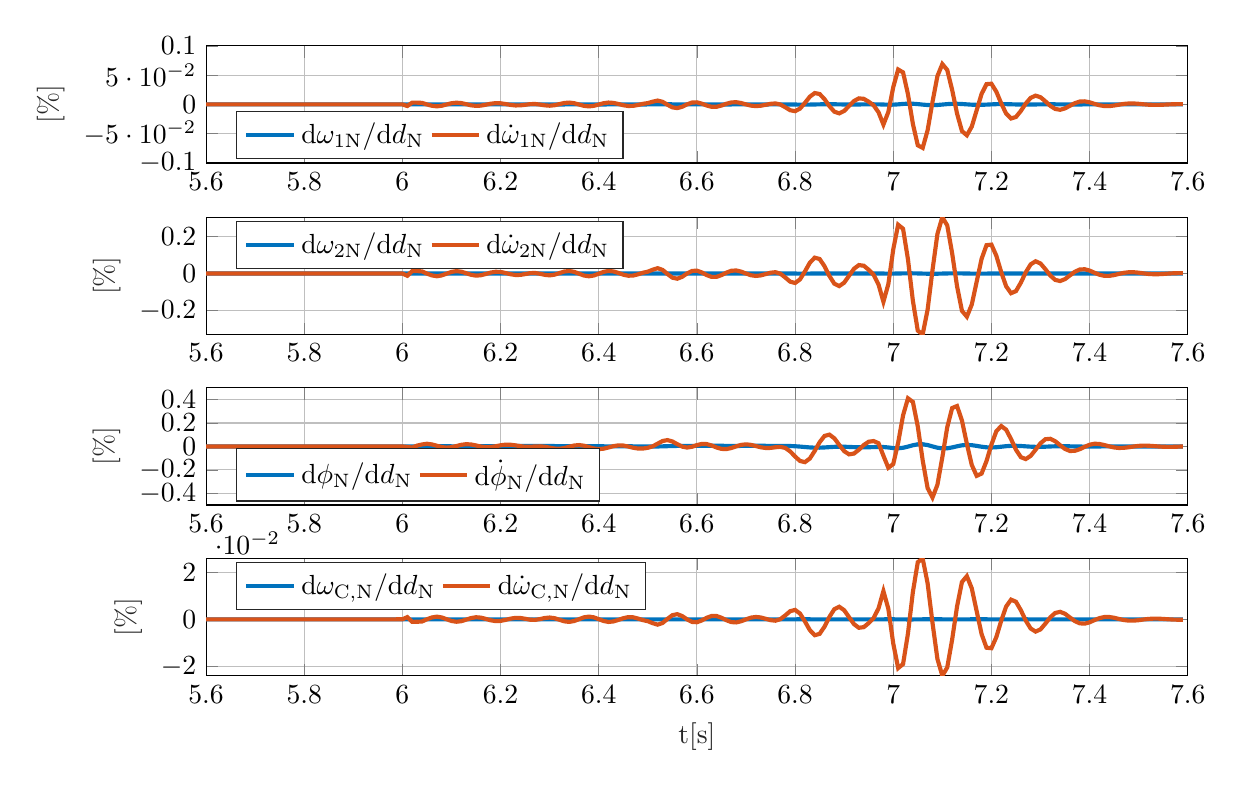
\begin{tikzpicture}

\begin{axis}[%
width=0.959\dwidth,
height=0.186\dheight,
at={(0\dwidth,0.814\dheight)},
scale only axis,
xmin=5.6,
xmax=7.6,
ymin=-0.1,
ymax=0.1,
ylabel style={font=\color{white!15!black}},
ylabel={[$\%$]},
axis background/.style={fill=white},
xmajorgrids,
ymajorgrids,
legend style={at={(0.03,0.03)}, anchor=south west, legend columns=2, legend cell align=left, align=left, draw=white!15!black}
]
\addplot [color=mycolor1, line width=1.5pt]
  table[row sep=crcr]{%
5.59	0\\
5.6	-4.30831767634006e-13\\
5.61	-9.82141155803885e-13\\
5.62	-1.45132344528616e-12\\
5.63	-2.01057116737164e-12\\
5.64	-2.45693386489609e-12\\
5.65	-2.97796650544282e-12\\
5.66	-3.39071158388908e-12\\
5.67	-3.89689463556598e-12\\
5.68	-4.3153423796627e-12\\
5.69	-4.83898141385465e-12\\
5.7	-5.27353213122402e-12\\
5.71	-4.58827469543543e-12\\
5.72	-1.83518348214983e-12\\
5.73	7.11539904284985e-13\\
5.74	-2.56802852090534e-13\\
5.75	-6.27338858011221e-12\\
5.76	-1.49069368140702e-11\\
5.77	-2.165603011614e-11\\
5.78	-2.22326704959997e-11\\
5.79	-1.59679600064292e-11\\
5.8	-5.81238545015398e-12\\
5.81	2.91326331542316e-12\\
5.82	5.90008818535518e-12\\
5.83	1.86040186864514e-12\\
5.84	-6.73042224831567e-12\\
5.85	-1.53016240452418e-11\\
5.86	-1.96501989842711e-11\\
5.87	-1.78065688709651e-11\\
5.88	-1.10524094100303e-11\\
5.89	-2.17846470106101e-12\\
5.9	5.22160685507638e-12\\
5.91	1.01408668320017e-11\\
5.92	7.2814729289131e-11\\
5.93	1.70499834569092e-09\\
5.94	2.44275902438312e-08\\
5.95	1.11205635648632e-07\\
5.96	2.57245268094344e-07\\
5.97	3.68497061346844e-07\\
5.98	3.17330271043247e-07\\
5.99	5.31802880659262e-08\\
6	-3.19585622998285e-07\\
6.01	-1.2959415665267e-05\\
6.02	-2.67691149595041e-05\\
6.03	2.17880803248147e-05\\
6.04	5.04164603662629e-05\\
6.05	6.80922126332615e-05\\
6.06	5.20418153974847e-05\\
6.07	1.89399958990366e-05\\
6.08	-1.55826620410975e-05\\
6.09	-3.04289153578281e-05\\
6.1	-1.95478134751785e-05\\
6.11	1.04615274404272e-05\\
6.12	4.17338630350636e-05\\
6.13	5.75921462770771e-05\\
6.14	5.01285468209688e-05\\
6.15	2.50491605811897e-05\\
6.16	-3.052808157494e-06\\
6.17	-1.88688717510645e-05\\
6.18	-1.48351905829751e-05\\
6.19	5.13813259497739e-06\\
6.2	2.96341626759476e-05\\
6.21	4.52358720322147e-05\\
6.22	4.41563808322684e-05\\
6.23	2.8466830571032e-05\\
6.24	7.51588737275339e-06\\
6.25	-7.02626024384875e-06\\
6.26	-7.67867568292319e-06\\
6.27	1.26765737493943e-07\\
6.28	3.4047038935846e-06\\
6.29	-7.56636213984137e-06\\
6.3	-3.07597257581592e-05\\
6.31	-5.30758248634155e-05\\
6.32	-5.86658803140156e-05\\
6.33	-4.08086358292052e-05\\
6.34	-7.20908784979998e-06\\
6.35	2.39903070259515e-05\\
6.36	3.5153712039654e-05\\
6.37	1.88993066948357e-05\\
6.38	-1.63103645169149e-05\\
6.39	-5.13642368758169e-05\\
6.4	-6.72457688288652e-05\\
6.41	-5.6398792398586e-05\\
6.42	-2.55419777170449e-05\\
6.43	8.27751098313268e-06\\
6.44	2.75918165747605e-05\\
6.45	2.34781048721751e-05\\
6.46	-1.35141185940008e-06\\
6.47	-3.26060904016496e-05\\
6.48	-5.34479052516628e-05\\
6.49	-5.34337496945309e-05\\
6.5	-3.39172239735319e-05\\
6.51	3.87956981737562e-06\\
6.52	7.12202681771509e-05\\
6.53	0.000137972632873364\\
6.54	0.000161613574276918\\
6.55	0.000126799853594793\\
6.56	5.7744432513692e-05\\
6.57	-4.78832003522571e-06\\
6.58	-2.7952714882798e-05\\
6.59	-7.55207541653974e-06\\
6.6	3.38368914021719e-05\\
6.61	6.37690573924369e-05\\
6.62	6.03098209633385e-05\\
6.63	2.38125105608474e-05\\
6.64	-2.5783207033256e-05\\
6.65	-6.19139958905386e-05\\
6.66	-6.68221069891359e-05\\
6.67	-4.00817382520885e-05\\
6.68	2.66640900720789e-06\\
6.69	3.94046617582281e-05\\
6.7	5.33244634444202e-05\\
6.71	4.04959162053505e-05\\
6.72	1.02239892806299e-05\\
6.73	-2.11766926736998e-05\\
6.74	-3.9072151754468e-05\\
6.75	-3.72374805127988e-05\\
6.76	-2.0090779300942e-05\\
6.77	-1.00142598343172e-05\\
6.78	-3.81877597053639e-05\\
6.79	-0.000125612740509086\\
6.8	-0.000255110632340129\\
6.81	-0.00036837939792308\\
6.82	-0.000398895297525212\\
6.83	-0.000307979944796254\\
6.84	-0.000114507201932795\\
6.85	0.000107424765535459\\
6.86	0.000266577314354131\\
6.87	0.000300745105658637\\
6.88	0.000206859341053337\\
6.89	3.96172438244971e-05\\
6.9	-0.000119164270300733\\
6.91	-0.000200886664279836\\
6.92	-0.000180649055044502\\
6.93	-8.3084081612616e-05\\
6.94	3.6017151293659e-05\\
6.95	0.000119911006960783\\
6.96	0.000136992458162182\\
6.97	8.25564503619923e-05\\
6.98	-0.000235867842339199\\
6.99	-0.000541900982840649\\
7	-0.000448218134451717\\
7.01	9.48953286433936e-05\\
7.02	0.000787725850237172\\
7.03	0.0012231625979619\\
7.04	0.0011309938552358\\
7.05	0.000508471212391878\\
7.06	-0.000354448284870544\\
7.07	-0.0010582889786163\\
7.08	-0.00129690976336356\\
7.09	-0.000975013560976583\\
7.1	-0.000274995167000601\\
7.11	0.000486747310051922\\
7.12	0.00097598239266593\\
7.13	0.00102719022437697\\
7.14	0.000657879438160034\\
7.15	6.59338384738917e-05\\
7.16	-0.000470774633826525\\
7.17	-0.000746249196295552\\
7.18	-0.000689508793064418\\
7.19	-0.000371212125992056\\
7.2	4.58263398431003e-05\\
7.21	0.000385574670531552\\
7.22	0.000518368219043633\\
7.23	0.000425980492310332\\
7.24	0.000187791939454705\\
7.25	-8.26381521762875e-05\\
7.26	-0.0002723732361666\\
7.27	-0.000320248083759635\\
7.28	-0.000239758377799904\\
7.29	-8.27066140114438e-05\\
7.3	7.98929492039389e-05\\
7.31	0.000184122513688753\\
7.32	0.000194459118269577\\
7.33	0.000132531824910331\\
7.34	3.1287410727672e-05\\
7.35	-6.38047870073148e-05\\
7.36	-0.000114865673980443\\
7.37	-0.000111714973952681\\
7.38	-6.91500764083011e-05\\
7.39	-9.15600581283641e-06\\
7.4	4.28752568580703e-05\\
7.41	6.94311147463029e-05\\
7.42	6.26772056643359e-05\\
7.43	3.6183059160036e-05\\
7.44	2.69154477283973e-06\\
7.45	-2.52018618994143e-05\\
7.46	-3.87512060652912e-05\\
7.47	-3.4517386049863e-05\\
7.48	-1.94829745099465e-05\\
7.49	-6.4472858473597e-07\\
7.5	1.47180428152034e-05\\
7.51	2.16138000257711e-05\\
7.52	1.85320021182538e-05\\
7.53	1.00427287157604e-05\\
7.54	1.11793719962074e-08\\
7.55	-7.78356324326664e-06\\
7.56	-1.09726232408441e-05\\
7.57	-9.55708890743882e-06\\
7.58	-5.26843792254145e-06\\
7.59	3.1916860888301e-08\\
};
\addlegendentry{d$\omega_{1\mathrm{N}}/$d$d_\mathrm{N}$}

\addplot [color=mycolor2, line width=1.5pt]
  table[row sep=crcr]{%
5.59	-4.98899172460086e-11\\
5.6	-3.25211340712767e-11\\
5.61	-5.42785142101515e-11\\
5.62	-3.51363707191503e-11\\
5.63	-5.39515631955255e-11\\
5.64	-3.24032393439167e-11\\
5.65	-5.04916387560489e-11\\
5.66	-2.98905317782809e-11\\
5.67	-4.98611666608069e-11\\
5.68	-3.09087507638327e-11\\
5.69	-5.15383302514616e-11\\
5.7	-3.20823309883498e-11\\
5.71	1.21949855075323e-10\\
5.72	2.97911110570443e-10\\
5.73	1.62883097257819e-10\\
5.74	-2.19984070496887e-10\\
5.75	-6.60125921308039e-10\\
5.76	-7.5989232469609e-10\\
5.77	-4.58302108284436e-10\\
5.78	1.74977700466346e-10\\
5.79	7.19689820490606e-10\\
5.8	9.35273571035191e-10\\
5.81	6.3935315266323e-10\\
5.82	6.62798139116329e-11\\
5.83	-5.34327807720652e-10\\
5.84	-7.93917604725937e-10\\
5.85	-6.60203016571779e-10\\
5.86	-1.71950634888627e-10\\
5.87	3.60894725122205e-10\\
5.88	7.47495509155084e-10\\
5.89	8.12793473475699e-10\\
5.9	6.52451280064071e-10\\
5.91	4.08360910682505e-10\\
5.92	2.30645109570623e-08\\
5.93	4.71587704325445e-07\\
5.94	4.19252372462251e-06\\
5.95	1.09697508773904e-05\\
5.96	1.30607544707775e-05\\
5.97	4.20791477213271e-06\\
5.98	-1.39752722483269e-05\\
5.99	-3.02861672169744e-05\\
6	-3.16074085469792e-05\\
6.01	-0.00272444404402052\\
6.02	0.00306660289606148\\
6.03	0.00297723383561637\\
6.04	0.00258891598577774\\
6.05	-9.64903967001968e-05\\
6.06	-0.00228381675086697\\
6.07	-0.00329760859237714\\
6.08	-0.00231586628536699\\
6.09	-0.000193116169226226\\
6.1	0.00199900894611586\\
6.11	0.00292426117668466\\
6.12	0.00224980616679111\\
6.13	0.000366967513705075\\
6.14	-0.00157327239561876\\
6.15	-0.00255427262400685\\
6.16	-0.00208376398605979\\
6.17	-0.000536244636968484\\
6.18	0.00118624110543633\\
6.19	0.002146718169662\\
6.2	0.00190964671664699\\
6.21	0.000671235564343844\\
6.22	-0.000828821250353229\\
6.23	-0.00176511348489549\\
6.24	-0.0016910513601129\\
6.25	-0.000720872133661512\\
6.26	0.000448766255104491\\
6.27	0.000712537837877697\\
6.28	-0.000269695315085232\\
6.29	-0.0016070292314795\\
6.3	-0.00222488237450772\\
6.31	-0.00139898085993134\\
6.32	0.00053699420556258\\
6.33	0.00244594257498005\\
6.34	0.00310250929379916\\
6.35	0.00203036038965083\\
6.36	-0.000241601553157289\\
6.37	-0.00246340823319312\\
6.38	-0.00335585757051968\\
6.39	-0.00242935462763715\\
6.4	-0.000200279960198517\\
6.41	0.00203467983304381\\
6.42	0.00316313747806166\\
6.43	0.00253199944439886\\
6.44	0.000726335546727614\\
6.45	-0.00140504277411816\\
6.46	-0.00268417700843464\\
6.47	-0.00248193002581887\\
6.48	-0.000970829815680307\\
6.49	0.000956185732577297\\
6.5	0.00225219259551452\\
6.51	0.00466707394169134\\
6.52	0.00650910021481602\\
6.53	0.00443002747734121\\
6.54	-0.000569050803672887\\
6.55	-0.00505173360522134\\
6.56	-0.0063300171990497\\
6.57	-0.00400291065871166\\
6.58	5.19457855735976e-05\\
6.59	0.00314206977372939\\
6.6	0.00354099565276627\\
6.61	0.00131594650448195\\
6.62	-0.00190645853347003\\
6.63	-0.00411392126371995\\
6.64	-0.00407459002697304\\
6.65	-0.0019223887778328\\
6.66	0.0010741640314381\\
6.67	0.00332029105531017\\
6.68	0.00375843175064164\\
6.69	0.0023582740533536\\
6.7	-1.87829208183695e-06\\
6.71	-0.00207872913511741\\
6.72	-0.00292280874489596\\
6.73	-0.0023010711700148\\
6.74	-0.00070546450501232\\
6.75	0.000973830531382013\\
6.76	0.00163414783924399\\
6.77	-0.000197332012594622\\
6.78	-0.00481318252723054\\
6.79	-0.0099388936850086\\
6.8	-0.0115620089857572\\
6.81	-0.00716302455518844\\
6.82	0.00244013003457478\\
6.83	0.0130948615212485\\
6.84	0.0193476314446542\\
6.85	0.0177576524550945\\
6.86	0.00889735968246694\\
6.87	-0.00301447589753206\\
6.88	-0.0124272585901705\\
6.89	-0.0153341407876014\\
6.9	-0.0111579285811837\\
6.91	-0.00264412044719487\\
6.92	0.00576964902160533\\
6.93	0.0103008165484387\\
6.94	0.00949909336310895\\
6.95	0.00458195102106744\\
6.96	-0.00155062345465285\\
6.97	-0.0133979389007247\\
6.98	-0.0344286849091058\\
6.99	-0.0129442203049414\\
7	0.0294080750200183\\
7.01	0.0595652226344242\\
7.02	0.0546553406988504\\
7.03	0.0173477552044194\\
7.04	-0.0332620246587181\\
7.05	-0.0697978337977169\\
7.06	-0.0742434269606503\\
7.07	-0.0442374571878472\\
7.08	0.00425439438677921\\
7.09	0.0482515351419329\\
7.1	0.068844138469317\\
7.11	0.0587875284833021\\
7.12	0.0247866017230693\\
7.13	-0.0155948028972907\\
7.14	-0.0455578823174211\\
7.15	-0.0527143262168949\\
7.16	-0.0378993314591196\\
7.17	-0.00995655140470502\\
7.18	0.0179059348922258\\
7.19	0.0345897367714203\\
7.2	0.035272480257382\\
7.21	0.0217671908270993\\
7.22	0.00172678198486632\\
7.23	-0.0155757095936112\\
7.24	-0.0240203644179055\\
7.25	-0.0214677247105953\\
7.26	-0.0111694673650278\\
7.27	0.00149771438286218\\
7.28	0.0111841535350316\\
7.29	0.0149596944482959\\
7.3	0.0122506197545902\\
7.31	0.00523937272104222\\
7.32	-0.00244468103537259\\
7.33	-0.00777587561185838\\
7.34	-0.00917288390788656\\
7.35	-0.0067903394218489\\
7.36	-0.00225403555859075\\
7.37	0.00213370274866475\\
7.38	0.00485962058494995\\
7.39	0.00525088810404354\\
7.4	0.00361846109969423\\
7.41	0.000944436328077961\\
7.42	-0.00145944279092249\\
7.43	-0.00279097917415653\\
7.44	-0.00287950549522102\\
7.45	-0.00191260698799216\\
7.46	-0.000446096563656461\\
7.47	0.000865920994425859\\
7.48	0.00158673653820018\\
7.49	0.00159121465351968\\
7.5	0.00101086651736129\\
7.51	0.000175377089979438\\
7.52	-0.000511584869468801\\
7.53	-0.000855771911937585\\
7.54	-0.000838596987113826\\
7.55	-0.00051482484109793\\
7.56	-8.75152070895476e-05\\
7.57	0.00026649597617993\\
7.58	0.000454162181832091\\
7.59	0.000442377709166627\\
};
\addlegendentry{d$\dot{\omega}_{1\mathrm{N}}/$d$d_\mathrm{N}$}

\end{axis}

\begin{axis}[%
width=0.959\dwidth,
height=0.186\dheight,
at={(0\dwidth,0.542\dheight)},
scale only axis,
xmin=5.6,
xmax=7.6,
ymin=-0.327126119151431,
ymax=0.303336157364176,
ylabel style={font=\color{white!15!black}},
ylabel={[$\%$]},
axis background/.style={fill=white},
xmajorgrids,
ymajorgrids,
legend style={at={(0.03,0.97)}, anchor=north west, legend columns=2, legend cell align=left, align=left, draw=white!15!black}
]
\addplot [color=mycolor1, line width=1.5pt]
  table[row sep=crcr]{%
5.59	0\\
5.6	-4.05003529267988e-13\\
5.61	-9.23231508307734e-13\\
5.62	-1.36429107796719e-12\\
5.63	-1.89000841233135e-12\\
5.64	-2.30958621113337e-12\\
5.65	-2.79935063210531e-12\\
5.66	-3.18731820747639e-12\\
5.67	-3.66311011591371e-12\\
5.68	-4.05645308687765e-12\\
5.69	-4.54867001668629e-12\\
5.7	-4.95712485710965e-12\\
5.71	-4.3130445805491e-12\\
5.72	-1.72524699265175e-12\\
5.73	6.68580910241625e-13\\
5.74	-2.41661627315677e-13\\
5.75	-5.8970621357139e-12\\
5.76	-1.40123206786574e-11\\
5.77	-2.03562663644601e-11\\
5.78	-2.08983060830011e-11\\
5.79	-1.50096762249082e-11\\
5.8	-5.46374978614659e-12\\
5.81	2.73805558915728e-12\\
5.82	5.54556279331524e-12\\
5.83	1.7483688237063e-12\\
5.84	-6.32675079702913e-12\\
5.85	-1.4383400440695e-11\\
5.86	-1.8470925798312e-11\\
5.87	-1.6737989674342e-11\\
5.88	-1.03893089948536e-11\\
5.89	-2.04807495262096e-12\\
5.9	4.90773625866457e-12\\
5.91	9.53166851841528e-12\\
5.92	6.8443067626691e-11\\
5.93	1.60264333553865e-09\\
5.94	2.29611513485726e-08\\
5.95	1.04529732370749e-07\\
5.96	2.41802305609447e-07\\
5.97	3.46375425132554e-07\\
5.98	2.98280282488919e-07\\
5.99	4.99877657542033e-08\\
6	-3.00400241788632e-07\\
6.01	-1.21814353143114e-05\\
6.02	-2.51621099419311e-05\\
6.03	2.04800970558283e-05\\
6.04	4.73898566212704e-05\\
6.05	6.40044971934259e-05\\
6.06	4.89176383295751e-05\\
6.07	1.78029890428787e-05\\
6.08	-1.46472026142815e-05\\
6.09	-2.86022049667065e-05\\
6.1	-1.83743178755681e-05\\
6.11	9.83350059081518e-06\\
6.12	3.92284936276739e-05\\
6.13	5.41347714720899e-05\\
6.14	4.71192272480317e-05\\
6.15	2.35454080783015e-05\\
6.16	-2.86954173594049e-06\\
6.17	-1.77361345340978e-05\\
6.18	-1.3944603536256e-05\\
6.19	4.82967989446194e-06\\
6.2	2.78551629244342e-05\\
6.21	4.25202696271506e-05\\
6.22	4.15055825049222e-05\\
6.23	2.67579082183092e-05\\
6.24	7.06469319163397e-06\\
6.25	-6.60445942516435e-06\\
6.26	-7.21770892894806e-06\\
6.27	1.19155796491361e-07\\
6.28	3.20031256567702e-06\\
6.29	-7.11213784093578e-06\\
6.3	-2.89131561595583e-05\\
6.31	-4.98895739447612e-05\\
6.32	-5.51440468802247e-05\\
6.33	-3.83588094824942e-05\\
6.34	-6.77631141548765e-06\\
6.35	2.25501196788869e-05\\
6.36	3.30433626520707e-05\\
6.37	1.77647428171867e-05\\
6.38	-1.53312194849436e-05\\
6.39	-4.82807358350454e-05\\
6.4	-6.32088668039681e-05\\
6.41	-5.3013056656396e-05\\
6.42	-2.40086401279074e-05\\
6.43	7.78059514215461e-06\\
6.44	2.59354232072587e-05\\
6.45	2.20686660935398e-05\\
6.46	-1.27028372998383e-06\\
6.47	-3.06486796615198e-05\\
6.48	-5.02393175441832e-05\\
6.49	-5.02260118049322e-05\\
6.5	-3.18811032230773e-05\\
6.51	3.64667136954438e-06\\
6.52	6.69447692409415e-05\\
6.53	0.000129689852329974\\
6.54	0.000151911579436969\\
6.55	0.000119187797966707\\
6.56	5.42779157857621e-05\\
6.57	-4.50086721129404e-06\\
6.58	-2.62746558771885e-05\\
6.59	-7.09870871664446e-06\\
6.6	3.1805593402078e-05\\
6.61	5.99408699709458e-05\\
6.62	5.668929861192e-05\\
6.63	2.23829967456338e-05\\
6.64	-2.4235388031729e-05\\
6.65	-5.81971713937226e-05\\
6.66	-6.28106384979545e-05\\
6.67	-3.7675549033168e-05\\
6.68	2.50633910931094e-06\\
6.69	3.70391190612668e-05\\
6.7	5.01232864523815e-05\\
6.71	3.80648632630836e-05\\
6.72	9.61022231286533e-06\\
6.73	-1.99054121832255e-05\\
6.74	-3.67265700898487e-05\\
6.75	-3.50020379328457e-05\\
6.76	-1.8884688579149e-05\\
6.77	-9.41308371606627e-06\\
6.78	-3.5895270886956e-05\\
6.79	-0.000118071950730522\\
6.8	-0.000239795818085508\\
6.81	-0.000346264826802921\\
6.82	-0.000374948794048706\\
6.83	-0.000289491277018449\\
6.84	-0.00010763310052762\\
6.85	0.000100975834912424\\
6.86	0.000250574129219983\\
6.87	0.000282690757813348\\
6.88	0.00019444114856228\\
6.89	3.72389380672504e-05\\
6.9	-0.000112010595509199\\
6.91	-0.000188827026267692\\
6.92	-0.000169804322297944\\
6.93	-7.80963746929659e-05\\
6.94	3.38549664789898e-05\\
6.95	0.000112712501608685\\
6.96	0.00012876851819619\\
6.97	7.76004158014616e-05\\
6.98	-0.000221708212248292\\
6.99	-0.000509369554493256\\
7	-0.000421310679999675\\
7.01	8.9198565974563e-05\\
7.02	0.000740437047748107\\
7.03	0.00114973363269022\\
7.04	0.00106309796895736\\
7.05	0.00047794663936344\\
7.06	-0.000333170027356589\\
7.07	-0.000994757718151963\\
7.08	-0.00121905360686635\\
7.09	-0.000916481494869271\\
7.1	-0.000258486643440558\\
7.11	0.000457526867510836\\
7.12	0.000917392162953098\\
7.13	0.000965525883277263\\
7.14	0.000618385582338199\\
7.15	6.1975693270581e-05\\
7.16	-0.00044251306678612\\
7.17	-0.000701450325330977\\
7.18	-0.000648116164891352\\
7.19	-0.000348927500630104\\
7.2	4.30752892917002e-05\\
7.21	0.000362427829504819\\
7.22	0.000487249508454281\\
7.23	0.000400408006780002\\
7.24	0.000176518402076788\\
7.25	-7.76772157032241e-05\\
7.26	-0.000256022112767669\\
7.27	-0.000301022934893343\\
7.28	-0.000225365191367538\\
7.29	-7.77415676682618e-05\\
7.3	7.50968096660132e-05\\
7.31	0.000173069258921623\\
7.32	0.000182785335941539\\
7.33	0.000124575665187456\\
7.34	2.94091611607556e-05\\
7.35	-5.99744565441658e-05\\
7.36	-0.00010797005356385\\
7.37	-0.000105008496534016\\
7.38	-6.49988572342287e-05\\
7.39	-8.60635394759002e-06\\
7.4	4.03013651147233e-05\\
7.41	6.52630202855956e-05\\
7.42	5.8914562243483e-05\\
7.43	3.40109137445898e-05\\
7.44	2.52996369291492e-06\\
7.45	-2.3688944464106e-05\\
7.46	-3.64248935283155e-05\\
7.47	-3.24452384347942e-05\\
7.48	-1.83133735076061e-05\\
7.49	-6.06026171705509e-07\\
7.5	1.38344864950135e-05\\
7.51	2.03162772308166e-05\\
7.52	1.74194859840656e-05\\
7.53	9.43984108284203e-06\\
7.54	1.05062389207755e-08\\
7.55	-7.31630197244438e-06\\
7.56	-1.03139161533206e-05\\
7.57	-8.98335925437063e-06\\
7.58	-4.95216480016493e-06\\
7.59	2.99988039650026e-08\\
};
\addlegendentry{d$\omega_{2\mathrm{N}}/$d$d_\mathrm{N}$}

\addplot [color=mycolor2, line width=1.5pt]
  table[row sep=crcr]{%
5.59	-2.19823363257795e-10\\
5.6	-1.43292024156739e-10\\
5.61	-2.39168058204528e-10\\
5.62	-1.54812445029881e-10\\
5.63	-2.37724499734465e-10\\
5.64	-1.42774811833676e-10\\
5.65	-2.22486200984853e-10\\
5.66	-1.31711647286073e-10\\
5.67	-2.19704187588456e-10\\
5.68	-1.36175838888446e-10\\
5.69	-2.27080333151836e-10\\
5.7	-1.41344857375996e-10\\
5.71	5.37320732384139e-10\\
5.72	1.31264205237236e-09\\
5.73	7.17691818643507e-10\\
5.74	-9.69278588343697e-10\\
5.75	-2.90860518627617e-09\\
5.76	-3.34819048030923e-09\\
5.77	-2.01932825543543e-09\\
5.78	7.70974998695937e-10\\
5.79	3.17104735409157e-09\\
5.8	4.1209287092497e-09\\
5.81	2.81708347476967e-09\\
5.82	2.92031962333878e-10\\
5.83	-2.35432428222806e-09\\
5.84	-3.49809579451684e-09\\
5.85	-2.90893453697864e-09\\
5.86	-7.57636981411544e-10\\
5.87	1.59013714730041e-09\\
5.88	3.29356544507792e-09\\
5.89	3.58126191761757e-09\\
5.9	2.87478106107014e-09\\
5.91	1.79928941917433e-09\\
5.92	1.01625202931355e-07\\
5.93	2.07787627808879e-06\\
5.94	1.84728005034876e-05\\
5.95	4.83341378474538e-05\\
5.96	5.75473694901049e-05\\
5.97	1.85406154469344e-05\\
5.98	-6.1576852819062e-05\\
5.99	-0.000133444760728205\\
6	-0.000139266320499388\\
6.01	-0.0120042520052118\\
6.02	0.0135118480575867\\
6.03	0.0131180764455706\\
6.04	0.0114070978927906\\
6.05	-0.000425149138449178\\
6.06	-0.0100627912954518\\
6.07	-0.0145296889632518\\
6.08	-0.0102040056799482\\
6.09	-0.000850894760256931\\
6.1	0.00880789135766455\\
6.11	0.012884672075035\\
6.12	0.0099129362734748\\
6.13	0.00161690621684761\\
6.14	-0.00693204118150148\\
6.15	-0.0112544547706529\\
6.16	-0.00918133300001954\\
6.17	-0.00236276306454215\\
6.18	0.00522673137655952\\
6.19	0.00945871725622453\\
6.2	0.00841414984382922\\
6.21	0.00295755050903856\\
6.22	-0.0036518933755888\\
6.23	-0.00777731777497329\\
6.24	-0.00745099049659928\\
6.25	-0.00317625563828463\\
6.26	0.00197732202631894\\
6.27	0.00313953365563837\\
6.28	-0.001188312358272\\
6.29	-0.00708077815609718\\
6.3	-0.00980311882864134\\
6.31	-0.00616409018564069\\
6.32	0.00236606576048301\\
6.33	0.0107771385963022\\
6.34	0.0136700562791832\\
6.35	0.00894602986333149\\
6.36	-0.00106452761814142\\
6.37	-0.0108540945400821\\
6.38	-0.0147863414770877\\
6.39	-0.010704049959904\\
6.4	-0.000882459347656749\\
6.41	0.00896506188826921\\
6.42	0.0139371918821679\\
6.43	0.0111563162672757\\
6.44	0.00320032814120808\\
6.45	-0.00619079976175083\\
6.46	-0.0118268302505892\\
6.47	-0.0109357039483433\\
6.48	-0.00427760143842111\\
6.49	0.00421307771866356\\
6.5	0.00992345118636321\\
6.51	0.0205637300006078\\
6.52	0.0286799354448959\\
6.53	0.019519272691509\\
6.54	-0.00250731126817115\\
6.55	-0.0222585901124827\\
6.56	-0.0278908725695515\\
6.57	-0.0176373408758298\\
6.58	0.000228879834043181\\
6.59	0.0138443648584205\\
6.6	0.0156020837566531\\
6.61	0.00579823010122658\\
6.62	-0.00840010229737922\\
6.63	-0.0181264679256902\\
6.64	-0.0179531694214912\\
6.65	-0.00847029300960673\\
6.66	0.00473290532672635\\
6.67	0.0146296308217702\\
6.68	0.0165601352606557\\
6.69	0.0103908597777616\\
6.7	-8.2759972673005e-06\\
6.71	-0.00915914879708469\\
6.72	-0.0128782724731368\\
6.73	-0.010138816492643\\
6.74	-0.00310836763834476\\
6.75	0.00429082297898705\\
6.76	0.00720026624113955\\
6.77	-0.00086947031012877\\
6.78	-0.0212075032815378\\
6.79	-0.0437920480362363\\
6.8	-0.0509437034891891\\
6.81	-0.0315612104673806\\
6.82	0.010751527793292\\
6.83	0.0576976495514165\\
6.84	0.0852481606569103\\
6.85	0.0782425080667899\\
6.86	0.0392029148272354\\
6.87	-0.0132821697759048\\
6.88	-0.0547561048932847\\
6.89	-0.0675642029432375\\
6.9	-0.0491632730863282\\
6.91	-0.0116503358730807\\
6.92	0.0254218180728924\\
6.93	0.0453867268730306\\
6.94	0.0418542310685185\\
6.95	0.0201886674285443\\
6.96	-0.00683224702509764\\
6.97	-0.0590330475928371\\
6.98	-0.151697228197366\\
6.99	-0.0570339049144644\\
7	0.129575773194193\\
7.01	0.262452056895471\\
7.02	0.240818483543204\\
7.03	0.0764364478894275\\
7.04	-0.146556772594738\\
7.05	-0.3075382620407\\
7.06	-0.327126119151431\\
7.07	-0.194915944527443\\
7.08	0.0187454106317653\\
7.09	0.21260248994764\\
7.1	0.303336157364176\\
7.11	0.259025436116251\\
7.12	0.109212965518383\\
7.13	-0.0687127138329183\\
7.14	-0.200733908028727\\
7.15	-0.232266123277892\\
7.16	-0.166989344729845\\
7.17	-0.0438698502276697\\
7.18	0.0788958596183297\\
7.19	0.152406843483951\\
7.2	0.15541509938057\\
7.21	0.0959090515025864\\
7.22	0.00760842423974823\\
7.23	-0.0686285862732163\\
7.24	-0.105836825080788\\
7.25	-0.0945895651518196\\
7.26	-0.049214114456861\\
7.27	0.0065991228277047\\
7.28	0.049278823616909\\
7.29	0.0659143440557459\\
7.3	0.0539778113912033\\
7.31	0.0230853522687082\\
7.32	-0.0107715800900199\\
7.33	-0.0342615113020105\\
7.34	-0.0404169101165413\\
7.35	-0.0299191116806509\\
7.36	-0.00993157151948145\\
7.37	0.00940136963187032\\
7.38	0.0214121153559561\\
7.39	0.0231360905320972\\
7.4	0.0159434065115447\\
7.41	0.00416130832636182\\
7.42	-0.00643049325526203\\
7.43	-0.0122974143739187\\
7.44	-0.0126874727674732\\
7.45	-0.00842719318137199\\
7.46	-0.00196555902132355\\
7.47	0.00381535963512165\\
7.48	0.00699136593106383\\
7.49	0.00701109708497969\\
7.5	0.00445400831214803\\
7.51	0.000772734088139325\\
7.52	-0.00225410894698848\\
7.53	-0.00377064146809142\\
7.54	-0.00369496653315354\\
7.55	-0.00226838468004014\\
7.56	-0.000385603294915023\\
7.57	0.00117421565822433\\
7.58	0.00200109717572607\\
7.59	0.00194917326857415\\
};
\addlegendentry{d$\dot{\omega}_{2\mathrm{N}}/$d$d_\mathrm{N}$}

\end{axis}

\begin{axis}[%
width=0.959\dwidth,
height=0.186\dheight,
at={(0\dwidth,0.271\dheight)},
scale only axis,
xmin=5.6,
xmax=7.6,
ymin=-0.5,
ymax=0.5,
ylabel style={font=\color{white!15!black}},
ylabel={[$\%$]},
axis background/.style={fill=white},
xmajorgrids,
ymajorgrids,
legend style={at={(0.03,0.03)}, anchor=south west, legend columns=2, legend cell align=left, align=left, draw=white!15!black}
]
\addplot [color=mycolor1, line width=1.5pt]
  table[row sep=crcr]{%
5.59	-1.7571785426454e-05\\
5.6	-1.75880567631243e-05\\
5.61	-1.76043326335801e-05\\
5.62	-1.76206133210849e-05\\
5.63	-1.76368987213157e-05\\
5.64	-1.76531888166438e-05\\
5.65	-1.76694833011856e-05\\
5.66	-1.76857821378237e-05\\
5.67	-1.77020851573085e-05\\
5.68	-1.77183925190561e-05\\
5.69	-1.77347041974616e-05\\
5.7	-1.77510203813149e-05\\
5.71	-1.77673346592354e-05\\
5.72	-1.77836293025331e-05\\
5.73	-1.77998969145635e-05\\
5.74	-1.78161609151703e-05\\
5.75	-1.78324655063774e-05\\
5.76	-1.78488455802864e-05\\
5.77	-1.78652980803258e-05\\
5.78	-1.78817775205067e-05\\
5.79	-1.78982187262815e-05\\
5.8	-1.79145740605262e-05\\
5.81	-1.79308388962907e-05\\
5.82	-1.79470555821492e-05\\
5.83	-1.79632878642895e-05\\
5.84	-1.79795891298205e-05\\
5.85	-1.79959739180517e-05\\
5.86	-1.80124155380852e-05\\
5.87	-1.80288595220202e-05\\
5.88	-1.8045254640643e-05\\
5.89	-1.80615702715322e-05\\
5.9	-1.80778105458207e-05\\
5.91	-1.80939954799202e-05\\
5.92	-1.81100498676361e-05\\
5.93	-1.81211561167621e-05\\
5.94	-1.80454627085444e-05\\
5.95	-1.74813969647824e-05\\
5.96	-1.57765618084109e-05\\
5.97	-1.27481980715381e-05\\
5.98	-9.35050118526162e-06\\
5.99	-7.4708067379704e-06\\
6	-8.90745923033753e-06\\
6.01	-4.59330691756846e-05\\
6.02	-0.000296287362250685\\
6.03	-0.000314020730011289\\
6.04	3.07453194493806e-05\\
6.05	0.000619922103738984\\
6.06	0.00120863693439304\\
6.07	0.0015547067360528\\
6.08	0.00156187245829533\\
6.09	0.00132432521428081\\
6.1	0.00106712515979891\\
6.11	0.00101530672649506\\
6.12	0.00126822459519299\\
6.13	0.00175573268225603\\
6.14	0.00228416159602165\\
6.15	0.00264956264113954\\
6.16	0.00274992017817524\\
6.17	0.00263227471462845\\
6.18	0.00245850590391019\\
6.19	0.00240632023506295\\
6.2	0.0025727267533162\\
6.21	0.00293818681721887\\
6.22	0.00337511956815477\\
6.23	0.00372659910374524\\
6.24	0.00389641840899261\\
6.25	0.00388973664542247\\
6.26	0.00380970056806261\\
6.27	0.00377179352027374\\
6.28	0.00379581752206061\\
6.29	0.0037845271449667\\
6.3	0.00360862506627468\\
6.31	0.00320543023783025\\
6.32	0.00265827995074199\\
6.33	0.00216907495563362\\
6.34	0.00193517421494992\\
6.35	0.00202306468865094\\
6.36	0.002321988455186\\
6.37	0.00259942446558048\\
6.38	0.00262016794332361\\
6.39	0.00229195955347078\\
6.4	0.00170924446911483\\
6.41	0.00111349840963506\\
6.42	0.000719783916724749\\
6.43	0.000663089588006176\\
6.44	0.000846385480604075\\
6.45	0.00110757930790725\\
6.46	0.00122448823154071\\
6.47	0.00106284562153678\\
6.48	0.00064116324473768\\
6.49	0.000116861952352376\\
6.5	-0.000308905639251122\\
6.51	-0.000472002610148109\\
6.52	-0.000131299871009687\\
6.53	0.000877061607290799\\
6.54	0.0023400129107988\\
6.55	0.00374128839318238\\
6.56	0.00462704816211299\\
6.57	0.00485819615376562\\
6.58	0.00466538650565402\\
6.59	0.00446807156019049\\
6.6	0.00458676413302569\\
6.61	0.00506971479912994\\
6.62	0.00568734406751065\\
6.63	0.00610622143083818\\
6.64	0.00609649303205964\\
6.65	0.00566085707108913\\
6.66	0.00502291194134529\\
6.67	0.00449496899353623\\
6.68	0.00431348627384486\\
6.69	0.00452548175002075\\
6.7	0.00498650389442822\\
6.71	0.00545013967103359\\
6.72	0.00569807884105298\\
6.73	0.00564042266929001\\
6.74	0.00534019221664141\\
6.75	0.00496545296609172\\
6.76	0.00470056528271591\\
6.77	0.00458013684306464\\
6.78	0.00438521030982424\\
6.79	0.00363469652250587\\
6.8	0.00180836352458573\\
6.81	-0.00119387117713212\\
6.82	-0.00491090562320171\\
6.83	-0.00835901445444882\\
6.84	-0.0104198424473884\\
6.85	-0.0104392322260772\\
6.86	-0.00858557895212908\\
6.87	-0.00578695928789343\\
6.88	-0.00329344672625304\\
6.89	-0.00209869241585206\\
6.9	-0.00251196292806306\\
6.91	-0.00410688759931998\\
6.92	-0.00599227090371682\\
6.93	-0.0072834862385868\\
6.94	-0.00749857822468321\\
6.95	-0.00671410162251095\\
6.96	-0.00544004260030165\\
6.97	-0.00432571816303428\\
6.98	-0.00487814823483425\\
6.99	-0.00877909241540059\\
7	-0.0138337537898627\\
7.01	-0.0157032705339313\\
7.02	-0.0112523154910139\\
7.03	-0.00135981319151633\\
7.04	0.0102620195895472\\
7.05	0.0182721606874711\\
7.06	0.0190454266507946\\
7.07	0.0119777659318817\\
7.08	0.000377159663326758\\
7.09	-0.0107226648672958\\
7.1	-0.0168082255703958\\
7.11	-0.0157223183088927\\
7.12	-0.0084084686058912\\
7.13	0.00136941475391727\\
7.14	0.00962584349138544\\
7.15	0.0129515003808737\\
7.16	0.0108214695269149\\
7.17	0.00476941252856272\\
7.18	-0.00225515339909659\\
7.19	-0.00737784322276277\\
7.2	-0.00892631628127126\\
7.21	-0.00676105859604274\\
7.22	-0.00229011954205376\\
7.23	0.00230848111750164\\
7.24	0.00526992769899013\\
7.25	0.00565872076919302\\
7.26	0.00384289485368346\\
7.27	0.000898452763397902\\
7.28	-0.00182188639199548\\
7.29	-0.00339296755628963\\
7.3	-0.00338961353669463\\
7.31	-0.00208442800754584\\
7.32	-0.000219174228860659\\
7.33	0.00137230481624511\\
7.34	0.00215980133498243\\
7.35	0.00198409715605352\\
7.36	0.00107935878076145\\
7.37	-3.14686713460342e-05\\
7.38	-0.000906994934249483\\
7.39	-0.00128054793015747\\
7.4	-0.00111220739167186\\
7.41	-0.000564621319643089\\
7.42	7.23910917262101e-05\\
7.43	0.000534419037409309\\
7.44	0.000717664900009621\\
7.45	0.000608077072200597\\
7.46	0.000302545912077645\\
7.47	-5.2011520371128e-05\\
7.48	-0.000309666536748744\\
7.49	-0.000404754373723377\\
7.5	-0.000333511244508927\\
7.51	-0.000154271752876454\\
7.52	3.79143462506807e-05\\
7.53	0.000169985207528824\\
7.54	0.000217106973652519\\
7.55	0.000173580613423922\\
7.56	7.92274042775023e-05\\
7.57	-2.02907088013351e-05\\
7.58	-9.16937374850691e-05\\
7.59	-0.000116437048036679\\
};
\addlegendentry{d$\phi_\mathrm{N}/$d$d_\mathrm{N}$}

\addplot [color=mycolor2, line width=1.5pt]
  table[row sep=crcr]{%
5.59	-5.76432268004859e-07\\
5.6	-5.76573241496256e-07\\
5.61	-5.76754667197868e-07\\
5.62	-5.7690851693505e-07\\
5.63	-5.77092612440046e-07\\
5.64	-5.77238780750554e-07\\
5.65	-5.7741002421832e-07\\
5.66	-5.77544892711724e-07\\
5.67	-5.77711138408851e-07\\
5.68	-5.77847921993487e-07\\
5.69	-5.78020031063407e-07\\
5.7	-5.78162208529048e-07\\
5.71	-5.77928315030431e-07\\
5.72	-5.76999946779381e-07\\
5.73	-5.76140913966483e-07\\
5.74	-5.76462441632477e-07\\
5.75	-5.78479389557194e-07\\
5.76	-5.81375177018543e-07\\
5.77	-5.83637995959356e-07\\
5.78	-5.83827749586058e-07\\
5.79	-5.81719845369803e-07\\
5.8	-5.78305267201196e-07\\
5.81	-5.7537104237531e-07\\
5.82	-5.74364268385862e-07\\
5.83	-5.75717360800425e-07\\
5.84	-5.78598900429234e-07\\
5.85	-5.81473756404381e-07\\
5.86	-5.82930374719923e-07\\
5.87	-5.82307322975127e-07\\
5.88	-5.80035103017288e-07\\
5.89	-5.77051021023628e-07\\
5.9	-5.74562033922336e-07\\
5.91	-5.72906293168893e-07\\
5.92	-5.51853604758115e-07\\
5.93	-3.68062642712023e-09\\
5.94	7.62769092078261e-06\\
5.95	3.67718094056963e-05\\
5.96	8.58179661689553e-05\\
5.97	0.000123179142174964\\
5.98	0.000105991086034042\\
5.99	1.72734414722352e-05\\
6	-0.000107919823615411\\
6.01	-0.00435301303450364\\
6.02	-0.00899079073218774\\
6.03	0.00731733223710111\\
6.04	0.0169319179585176\\
6.05	0.0228677726306885\\
6.06	0.0174765820354619\\
6.07	0.00635886252131942\\
6.08	-0.00523569959474132\\
6.09	-0.0102216186989489\\
6.1	-0.00656689467288171\\
6.11	0.00351190275068149\\
6.12	0.0140145654586557\\
6.13	0.0193401212261019\\
6.14	0.0168328984088633\\
6.15	0.00840952105794134\\
6.16	-0.00102872585724078\\
6.17	-0.00634048176774749\\
6.18	-0.00498557276615581\\
6.19	0.00172259457454209\\
6.2	0.00994950160087416\\
6.21	0.0151890126983559\\
6.22	0.0148260096620335\\
6.23	0.00955625608475787\\
6.24	0.00251963456970189\\
6.25	-0.00236438638137906\\
6.26	-0.00258341538955999\\
6.27	3.8112579721272e-05\\
6.28	0.00113899800598355\\
6.29	-0.00254565791489096\\
6.3	-0.010335043652048\\
6.31	-0.01782955975724\\
6.32	-0.0197064251025944\\
6.33	-0.0137084931039746\\
6.34	-0.00242372022079054\\
6.35	0.00805461618240812\\
6.36	0.0118035742325619\\
6.37	0.00634418685395043\\
6.38	-0.0054811245396586\\
6.39	-0.0172537449739333\\
6.4	-0.0225870010687985\\
6.41	-0.0189433802361569\\
6.42	-0.00857959697209096\\
6.43	0.00277885732561741\\
6.44	0.00926544312125801\\
6.45	0.00788356529845761\\
6.46	-0.000455637024948669\\
6.47	-0.0109524601147339\\
6.48	-0.0179518133960066\\
6.49	-0.0179465081164797\\
6.5	-0.011391366984636\\
6.51	0.0013029902402283\\
6.52	0.0239192421513281\\
6.53	0.0463371983394456\\
6.54	0.0542755537802934\\
6.55	0.0425817710325466\\
6.56	0.0193883360915568\\
6.57	-0.00161374806617524\\
6.58	-0.00939338415361796\\
6.59	-0.00254154548860111\\
6.6	0.011358963749039\\
6.61	0.0214112823322669\\
6.62	0.0202488392442457\\
6.63	0.00799065268416313\\
6.64	-0.00866622777752948\\
6.65	-0.0208004152940431\\
6.66	-0.0224481434602065\\
6.67	-0.0134667348086143\\
6.68	0.000890576547662198\\
6.69	0.0132290281676833\\
6.7	0.0179035598968409\\
6.71	0.0135945620673917\\
6.72	0.0034273719440401\\
6.73	-0.00711859150892594\\
6.74	-0.0131285220739204\\
6.75	-0.0125119404183316\\
6.76	-0.00675287606213829\\
6.77	-0.00336851015924597\\
6.78	-0.0128304692231835\\
6.79	-0.0421916594240343\\
6.8	-0.0856820477962898\\
6.81	-0.123720584726165\\
6.82	-0.133965526587699\\
6.83	-0.103427642584804\\
6.84	-0.0384469685667047\\
6.85	0.0360896743019511\\
6.86	0.0895396459336668\\
6.87	0.101012047842801\\
6.88	0.0694775374067306\\
6.89	0.0133074217413431\\
6.9	-0.0400194731127613\\
6.91	-0.067464539588094\\
6.92	-0.0606656734241631\\
6.93	-0.0278967709350538\\
6.94	0.0121040182942882\\
6.95	0.0402792258056443\\
6.96	0.0460147333389979\\
6.97	0.0277310208791068\\
6.98	-0.0792123166318625\\
6.99	-0.181990487766399\\
7	-0.150521414427029\\
7.01	0.0318871263472319\\
7.02	0.264571951237853\\
7.03	0.41080439006633\\
7.04	0.379836835438558\\
7.05	0.170751905352164\\
7.06	-0.119063450320839\\
7.07	-0.355443285778063\\
7.08	-0.435572556806876\\
7.09	-0.327450765540577\\
7.1	-0.0923406528665392\\
7.11	0.163492065990399\\
7.12	0.327795580971845\\
7.13	0.344983479819266\\
7.14	0.220940349370802\\
7.15	0.022129798056166\\
7.16	-0.158123346476053\\
7.17	-0.250635978426162\\
7.18	-0.231572010396935\\
7.19	-0.124665486091299\\
7.2	0.015399997375683\\
7.21	0.129503347692487\\
7.22	0.174097742943886\\
7.23	0.143064080748868\\
7.24	0.0630644517961338\\
7.25	-0.0277608573170979\\
7.26	-0.0914821045493008\\
7.27	-0.107557885264612\\
7.28	-0.0805222206717864\\
7.29	-0.0277741521457877\\
7.3	0.0268354764957024\\
7.31	0.0618399404595909\\
7.32	0.0653095237438645\\
7.33	0.0445093173702418\\
7.34	0.0105051810744138\\
7.35	-0.0214316777066541\\
7.36	-0.038579683458917\\
7.37	-0.0375203162630178\\
7.38	-0.0232238054867569\\
7.39	-0.00307418544097301\\
7.4	0.0144005150316119\\
7.41	0.0233188036047526\\
7.42	0.0210497939554089\\
7.43	0.0121511445255985\\
7.44	0.000902704882430644\\
7.45	-0.00846527539063476\\
7.46	-0.0130155407291645\\
7.47	-0.0115932154168339\\
7.48	-0.00654357800562998\\
7.49	-0.000216584777088219\\
7.5	0.00494297877750603\\
7.51	0.00725874945398466\\
7.52	0.00622350929722685\\
7.53	0.00337221436630361\\
7.54	3.03245066119838e-06\\
7.55	-0.00261481218870832\\
7.56	-0.00368576726171831\\
7.57	-0.00321024760917701\\
7.58	-0.00176981205924419\\
7.59	1.03572883532774e-05\\
};
\addlegendentry{d$\dot{\phi}_\mathrm{N}/$d$d_\mathrm{N}$}

\end{axis}

\begin{axis}[%
width=0.959\dwidth,
height=0.186\dheight,
at={(0\dwidth,0\dheight)},
scale only axis,
xmin=5.6,
xmax=7.6,
xlabel style={font=\color{white!15!black}},
xlabel={t[s]},
ymin=-0.0239121713006459,
ymax=0.0257692172916418,
ylabel style={font=\color{white!15!black}},
ylabel={[$\%$]},
axis background/.style={fill=white},
xmajorgrids,
ymajorgrids,
legend style={at={(0.03,0.97)}, anchor=north west, legend columns=2, legend cell align=left, align=left, draw=white!15!black}
]
\addplot [color=mycolor1, line width=1.5pt]
  table[row sep=crcr]{%
5.59	0\\
5.6	2.65224472006632e-15\\
5.61	9.05649238129227e-15\\
5.62	1.28871900836903e-14\\
5.63	1.95224053568151e-14\\
5.64	2.26223410908329e-14\\
5.65	2.80459805717028e-14\\
5.66	3.00802360660356e-14\\
5.67	3.50242362572319e-14\\
5.68	3.72210031101737e-14\\
5.69	4.26952124153148e-14\\
5.7	4.5377701642304e-14\\
5.71	1.31034959845666e-14\\
5.72	-8.36797133757089e-14\\
5.73	-1.7393395570579e-13\\
5.74	-1.54408657229899e-13\\
5.75	2.26388136440256e-14\\
5.76	2.81185840811048e-13\\
5.77	4.80678190687374e-13\\
5.78	4.87352721547641e-13\\
5.79	2.80514405868343e-13\\
5.8	-4.75621234862222e-14\\
5.81	-3.30712496165712e-13\\
5.82	-4.34513505526647e-13\\
5.83	-3.18943544310999e-13\\
5.84	-6.14583316453896e-14\\
5.85	1.95169604145075e-13\\
5.86	3.19776060932152e-13\\
5.87	2.51021138630773e-13\\
5.88	2.90785799295548e-14\\
5.89	-2.5881608000989e-13\\
5.9	-5.00457921591635e-13\\
5.91	-6.64463843888261e-13\\
5.92	-2.63153836837818e-12\\
5.93	-5.35938650005658e-11\\
5.94	-7.62873210016461e-10\\
5.95	-3.47091342960354e-09\\
5.96	-8.02607736403345e-09\\
5.97	-1.14910060725408e-08\\
5.98	-9.88310830930468e-09\\
5.99	-1.62906545482565e-09\\
6	1.0006756601562e-08\\
6.01	4.04591304305143e-07\\
6.02	8.35069756293666e-07\\
6.03	-6.81243531472704e-07\\
6.04	-1.57417079634655e-06\\
6.05	-2.1243580447213e-06\\
6.06	-1.62140490814615e-06\\
6.07	-5.86725771568519e-07\\
6.08	4.91306130802587e-07\\
6.09	9.5418421801748e-07\\
6.1	6.1363388078647e-07\\
6.11	-3.23604607377899e-07\\
6.12	-1.29936810964148e-06\\
6.13	-1.79310472793241e-06\\
6.14	-1.55846335915768e-06\\
6.15	-7.74236388370282e-07\\
6.16	1.03578235468917e-07\\
6.17	5.97094586749892e-07\\
6.18	4.70608545232315e-07\\
6.19	-1.53247602758902e-07\\
6.2	-9.17673600471556e-07\\
6.21	-1.40376429575284e-06\\
6.22	-1.36874838492567e-06\\
6.23	-8.77772489997214e-07\\
6.24	-2.23050533485401e-07\\
6.25	2.3101639662401e-07\\
6.26	2.51137387229461e-07\\
6.27	7.2780673928017e-09\\
6.28	-9.50172259018714e-08\\
6.29	2.47524441866326e-07\\
6.3	9.71226224344794e-07\\
6.31	1.66684821675312e-06\\
6.32	1.83974374736703e-06\\
6.33	1.28064308336926e-06\\
6.34	2.30741212068372e-07\\
6.35	-7.43239380333994e-07\\
6.36	-1.09093221113028e-06\\
6.37	-5.82534068334423e-07\\
6.38	5.16989418405002e-07\\
6.39	1.61059136804691e-06\\
6.4	2.1047420488927e-06\\
6.41	1.76422208665777e-06\\
6.42	7.99482489963408e-07\\
6.43	-2.56748173061862e-07\\
6.44	-8.59307966940293e-07\\
6.45	-7.30061768884128e-07\\
6.46	4.56239605009249e-08\\
6.47	1.02109803032601e-06\\
6.48	1.67062783771142e-06\\
6.49	1.66859218880063e-06\\
6.5	1.05787008817347e-06\\
6.51	-1.2287805108914e-07\\
6.52	-2.22464112398083e-06\\
6.53	-4.306003324009e-06\\
6.54	-5.03977492647602e-06\\
6.55	-3.94841456463017e-06\\
6.56	-1.78938425333014e-06\\
6.57	1.63973027187778e-07\\
6.58	8.86711208096599e-07\\
6.59	2.49061590667807e-07\\
6.6	-1.04301254243477e-06\\
6.61	-1.97622353716744e-06\\
6.62	-1.86633532281947e-06\\
6.63	-7.25397753130303e-07\\
6.64	8.2324666217201e-07\\
6.65	1.95013224913297e-06\\
6.66	2.10143311706972e-06\\
6.67	1.26480633965373e-06\\
6.68	-7.06254542146845e-08\\
6.69	-1.21718898420543e-06\\
6.7	-1.65045702636442e-06\\
6.71	-1.2484663451593e-06\\
6.72	-3.02443427933132e-07\\
6.73	6.77892234393757e-07\\
6.74	1.23576886966567e-06\\
6.75	1.17731970814434e-06\\
6.76	6.41069267714001e-07\\
6.77	3.26036612068927e-07\\
6.78	1.20518276278714e-06\\
6.79	3.93283471339079e-06\\
6.8	7.97097968416874e-06\\
6.81	1.1498757118077e-05\\
6.82	1.24402899195112e-05\\
6.83	9.59080646441665e-06\\
6.84	3.54308844800182e-06\\
6.85	-3.38705386733007e-06\\
6.86	-8.35109489335095e-06\\
6.87	-9.40943674664513e-06\\
6.88	-6.47008124518184e-06\\
6.89	-1.24406230625965e-06\\
6.9	3.71283592898992e-06\\
6.91	6.25984424937633e-06\\
6.92	5.62213304323357e-06\\
6.93	2.57160010768919e-06\\
6.94	-1.14812852387656e-06\\
6.95	-3.76539569348513e-06\\
6.96	-4.29485915113066e-06\\
6.97	-2.59159021780997e-06\\
6.98	7.34993644168039e-06\\
6.99	1.68942552416704e-05\\
7	1.39533906897029e-05\\
7.01	-3.0117322083612e-06\\
7.02	-2.46325399055794e-05\\
7.03	-3.8199177401754e-05\\
7.04	-3.52853535343476e-05\\
7.05	-1.58216739616765e-05\\
7.06	1.11264295802666e-05\\
7.07	3.30829630281817e-05\\
7.08	4.04984648798458e-05\\
7.09	3.04126640853119e-05\\
7.1	8.53497346745482e-06\\
7.11	-1.52480258440987e-05\\
7.12	-3.05024395919243e-05\\
7.13	-3.20713046514468e-05\\
7.14	-2.05136428440549e-05\\
7.15	-2.01914619659031e-06\\
7.16	1.47336608144394e-05\\
7.17	2.33170015047731e-05\\
7.18	2.15235101447944e-05\\
7.19	1.15684730917669e-05\\
7.2	-1.45885333538173e-06\\
7.21	-1.20612178157701e-05\\
7.22	-1.61940295859005e-05\\
7.23	-1.32948791991856e-05\\
7.24	-5.84798168601666e-06\\
7.25	2.59773518571847e-06\\
7.26	8.51682334297677e-06\\
7.27	1.00026527926384e-05\\
7.28	7.48083266645498e-06\\
7.29	2.57182801719596e-06\\
7.3	-2.50553301466465e-06\\
7.31	-5.75618139816463e-06\\
7.32	-6.07316664988675e-06\\
7.33	-4.13447107116158e-06\\
7.34	-9.70544644100712e-07\\
7.35	1.99828099918629e-06\\
7.36	3.58990983283006e-06\\
7.37	3.48807386918075e-06\\
7.38	2.15621145765394e-06\\
7.39	2.8166172161672e-07\\
7.4	-1.34255463442781e-06\\
7.41	-2.17009011770141e-06\\
7.42	-1.95720827308825e-06\\
7.43	-1.12845700168271e-06\\
7.44	-8.20726612032038e-08\\
7.45	7.88592184591962e-07\\
7.46	1.21073498707945e-06\\
7.47	1.07742396560956e-06\\
7.48	6.07152963682619e-07\\
7.49	1.86094054655078e-08\\
7.5	-4.60889445699078e-07\\
7.51	-6.75658368475672e-07\\
7.52	-5.78825268212403e-07\\
7.53	-3.13324475990329e-07\\
7.54	7.03629131500275e-11\\
7.55	2.43335038068535e-07\\
7.56	3.42622726861097e-07\\
7.57	2.98110082578466e-07\\
7.58	1.63968694957624e-07\\
7.59	-1.61845392386481e-09\\
};
\addlegendentry{d$\omega_{\mathrm{C,N}}/$d$d_\mathrm{N}$}

\addplot [color=mycolor2, line width=1.5pt]
  table[row sep=crcr]{%
5.59	6.90974614490037e-12\\
5.6	8.7237201716704e-13\\
5.61	8.41792207215707e-12\\
5.62	1.76256292843012e-12\\
5.63	8.28499680055005e-12\\
5.64	7.95953386229057e-13\\
5.65	7.06880778729951e-12\\
5.66	-9.13105631002499e-14\\
5.67	6.83392953562779e-12\\
5.68	2.45096496442047e-13\\
5.69	7.39988184487483e-12\\
5.7	6.37534753034844e-13\\
5.71	-5.28232347069743e-11\\
5.72	-1.138418924524e-10\\
5.73	-6.68832413670748e-11\\
5.74	6.60372505845657e-11\\
5.75	2.18709020104485e-10\\
5.76	2.53122265271759e-10\\
5.77	1.48223512834242e-10\\
5.78	-7.16776649799591e-11\\
5.79	-2.60641351486955e-10\\
5.8	-3.35217847459427e-10\\
5.81	-2.32225977216679e-10\\
5.82	-3.31531774601006e-11\\
5.83	1.7528779536645e-10\\
5.84	2.65195992458394e-10\\
5.85	2.18539379693573e-10\\
5.86	4.88932249235603e-11\\
5.87	-1.36068611134312e-10\\
5.88	-2.70119069653061e-10\\
5.89	-2.92545801176562e-10\\
5.9	-2.36666357782767e-10\\
5.91	-1.5177185458236e-10\\
5.92	-8.016867436456e-09\\
5.93	-1.63711366734824e-07\\
5.94	-1.45509874282079e-06\\
5.95	-3.80596651424337e-06\\
5.96	-4.52804271605836e-06\\
5.97	-1.45108053647156e-06\\
5.98	4.86119437211271e-06\\
5.99	1.05175551730089e-05\\
6	1.09661583258373e-05\\
6.01	0.00094564398240162\\
6.02	-0.00106553436211984\\
6.03	-0.00103317683598157\\
6.04	-0.000897561011156625\\
6.05	3.53641051114837e-05\\
6.06	0.000794420770894964\\
6.07	0.00114552943766395\\
6.08	0.000803698093599538\\
6.09	6.62179982431661e-05\\
6.1	-0.000694646237236128\\
6.11	-0.00101509527779501\\
6.12	-0.000780049939410489\\
6.13	-0.000125845244344535\\
6.14	0.000547650799654822\\
6.15	0.000887590508648596\\
6.16	0.000723445791206488\\
6.17	0.000185672581038985\\
6.18	-0.000412308011015158\\
6.19	-0.00074526128407826\\
6.2	-0.000662270359080052\\
6.21	-0.000231833118846822\\
6.22	0.000288995122584273\\
6.23	0.000613667452434704\\
6.24	0.000587373716091389\\
6.25	0.000250101569687927\\
6.26	-0.000156045065677816\\
6.27	-0.000247418063184934\\
6.28	9.37291647588242e-05\\
6.29	0.000557783421539369\\
6.3	0.00077167802206782\\
6.31	0.000484287954872113\\
6.32	-0.000188086303107488\\
6.33	-0.000850428335838972\\
6.34	-0.00107747604417775\\
6.35	-0.000704335478287678\\
6.36	8.4856936511476e-05\\
6.37	0.000855875556460177\\
6.38	0.00116478243225956\\
6.39	0.000842106524795845\\
6.4	6.76751301733826e-05\\
6.41	-0.000708059280597692\\
6.42	-0.00109903311983169\\
6.43	-0.000878947918285432\\
6.44	-0.000251439268999137\\
6.45	0.00048851597280339\\
6.46	0.000931975333782357\\
6.47	0.000860882662321957\\
6.48	0.000335611543821802\\
6.49	-0.000333496885310362\\
6.5	-0.000782961076012982\\
6.51	-0.00162041978655102\\
6.52	-0.00225814764753838\\
6.53	-0.00153438526367936\\
6.54	0.000202079272460843\\
6.55	0.0017576117297798\\
6.56	0.00219954131232844\\
6.57	0.00138976820773105\\
6.58	-1.88278206420126e-05\\
6.59	-0.00109123035837232\\
6.6	-0.0012285947838794\\
6.61	-0.000455166752742223\\
6.62	0.000663638194626766\\
6.63	0.00142910800074233\\
6.64	0.00141406798609352\\
6.65	0.000665760891399719\\
6.66	-0.000374855570332897\\
6.67	-0.00115402173227192\\
6.68	-0.00130496188244214\\
6.69	-0.000817765550111837\\
6.7	2.12827407128542e-06\\
6.71	0.000722905446785699\\
6.72	0.00101514560093355\\
6.73	0.000798385007900162\\
6.74	0.000243849604391242\\
6.75	-0.00033919304982928\\
6.76	-0.000567992437745593\\
6.77	6.82268670835842e-05\\
6.78	0.0016701826329184\\
6.79	0.00344751954649822\\
6.8	0.00400748985934026\\
6.81	0.00247688711409389\\
6.82	-0.000858422337710288\\
6.83	-0.00455546984752348\\
6.84	-0.00672117502449781\\
6.85	-0.00616288154220236\\
6.86	-0.00308190699523687\\
6.87	0.00105514177579368\\
6.88	0.00432086949508221\\
6.89	0.00532552749865258\\
6.9	0.00387099093227856\\
6.91	0.000912489360341201\\
6.92	-0.00200841849853342\\
6.93	-0.00357901966553545\\
6.94	-0.00329730057837613\\
6.95	-0.00158758989179111\\
6.96	0.000542275648162693\\
6.97	0.00465444113754442\\
6.98	0.0119479251029196\\
6.99	0.00447937692798976\\
7	-0.0102237981150206\\
7.01	-0.0206798806442428\\
7.02	-0.0189555804096523\\
7.03	-0.00598919682014866\\
7.04	0.0115812176219558\\
7.05	0.0242498725573035\\
7.06	0.0257692172916418\\
7.07	0.0153305713699907\\
7.08	-0.00151375248095773\\
7.09	-0.0167816151917344\\
7.1	-0.0239121713006459\\
7.11	-0.0203987939704762\\
7.12	-0.00857901487203884\\
7.13	0.00544388145089346\\
7.14	0.0158374085589433\\
7.15	0.018305606078433\\
7.16	0.013146314518986\\
7.17	0.00343609240535347\\
7.18	-0.00623686992325454\\
7.19	-0.0120209190354932\\
7.2	-0.0122462001622857\\
7.21	-0.00754721611141239\\
7.22	-0.000584921027855466\\
7.23	0.00542033155187718\\
7.24	0.00834579174465475\\
7.25	0.00745179681909897\\
7.26	0.00387060837546336\\
7.27	-0.00052911532552283\\
7.28	-0.00389021361077117\\
7.29	-0.00519672744681696\\
7.3	-0.00425145908007192\\
7.31	-0.00181402048329891\\
7.32	0.000854371740228955\\
7.33	0.00270374138218417\\
7.34	0.00318594513907633\\
7.35	0.00235596574381214\\
7.36	0.000779395741637609\\
7.37	-0.000744049182407725\\
7.38	-0.00168934789607721\\
7.39	-0.00182350089669113\\
7.4	-0.00125520151419671\\
7.41	-0.000325956885639933\\
7.42	0.000508539003888107\\
7.43	0.000970128463489332\\
7.44	0.00099991379769924\\
7.45	0.000663387872010952\\
7.46	0.000153792252517292\\
7.47	-0.000301653010254091\\
7.48	-0.000551510077245641\\
7.49	-0.000552528005362561\\
7.5	-0.000350578321031433\\
7.51	-6.02784593697495e-05\\
7.52	0.000178164281633396\\
7.53	0.000297432503604354\\
7.54	0.000291182554888718\\
7.55	0.0001785380474788\\
7.56	3.00741843900561e-05\\
7.57	-9.2807053340557e-05\\
7.58	-0.000157846954175034\\
7.59	-0.00015360354715461\\
};
\addlegendentry{d$\dot{\omega}_{\mathrm{C,N}}/$d$d_\mathrm{N}$}

\end{axis}
\end{tikzpicture}%
\caption{Normierte Sensitivitäten der Zustände und deren Ableitungen von $d_\mathrm{ss}$}
\label{fig:Sens_d}
\end{figure}

\subsection{Sensitivität des Zustandes $\pmb{x}$ von $m_\mathrm{veh}$}
Die Sensitivität von \eqref{eq:sys_nl23} vom Parameter $m_\mathrm{veh}$ ergibt sich mit \eqref{eq:Sens_eq} zu
\begin{equation}
\begin{split}
&\dot{\pmb{S}}_{m_\mathrm{C}} = \left. \pmb{J}_\mathrm{p}(t,\pmb{x}(t,\pmb{p}),\pmb{p}))\right|_{\pmb{p}=\pmb{p}_0} \pmb{S}_{m_\mathrm{C}} \\
&+ \begin{bmatrix} 0 \\ 0 \\ 0 \\ -\frac{10^{-8}(5,72\cdot 10^{2}\,\sin(\zeta) + 5,99\,\phi\,k_\mathrm{ss} + 2,42\,d_\mathrm{ss}\,\omega_2 - 5,99\,\omega_\mathrm{C} - 4,18\cdot 10^{-2}\,\omega_\mathrm{C}^2 + 1,88\cdot 10^{2}\,f_\mathrm{Roll}\,\omega_\mathrm{C}\,\cos(\zeta))}{(5.69\,m_\mathrm{veh} + 337)^2}\end{bmatrix}.
\end{split}
\end{equation}
Aufgrund der Widerstandsmomenten welche in \eqref{eq:Fr_Fas_Fg} definiert sind, ist $\pmb{S}_{m_\mathrm{C}}$ auch von der Fahrbahnsteigung $\zeta$ abhängig. In Abbildung \ref{fig:Sens_m} sind die Sensitivitäten der Zustände und deren Ableitungen zu $d_\mathrm{ss}$ abgebildet. Aus den Sensitivitätsverläufen der Ableitungen der Drehzahlen $\omega_1$, $\omega_2$ und $\omega_\mathrm{C}$ wird vor allem der direkte Bezug zu $a_\mathrm{C}$ ersichtlich. Beim Abfallen von $a_\mathrm{C}$ sinkt auch der Betrag der Sensitvitäten. Dieser Zusammenhang ergibt sich aus \eqref{eq:dynwc}, wo $m_\mathrm{C}$ in $I_\mathrm{C}^\mathrm{eff}$ eingeht. Folglich ergibt sich auch das Abfallen der Sensitivitätsverläufe von $\omega_1$, $\omega_2$ und $\omega_\mathrm{C}$, da eine positive Änderung der Masse eine Drehzahlabnahme zur Folge hätte und umgekehrt. Die positive Sensitivität $\frac{\partial \phi_\mathrm{N}}{\partial m_\mathrm{C,N}}$ lässt sich darauf zurückführen, dass das mit einer Erhöhung von $m_\mathrm{C}$ die Trägheit im Abtriebsstrang steigen würde und während der Beschleunigung das Widerstandsmoment, was zur positiven Verdrehung der Seitenwelle führen würde. Zusätzlich würde dabei auch $T_\mathrm{res}$ steigen was den Effekt noch verstärkt. Des Weiteren lässt sich am Schwingen aller Einträge von $\dot{\pmb{S}}_{m_\mathrm{C}}$ für $t>7\, s$ auch erkennen, dass die Schwingungen im Antriebsstrang beim abrupten schließen von $B_{05}$ auch von $m_\mathrm{C}$ abhängen.

\begin{figure}
\centering
\newlength\mheight 
\setlength\mheight{8cm}
\newlength\mwidth 
\setlength\mwidth{13cm}
% This file was created by matlab2tikz.
%
%The latest updates can be retrieved from
%  http://www.mathworks.com/matlabcentral/fileexchange/22022-matlab2tikz-matlab2tikz
%where you can also make suggestions and rate matlab2tikz.
%
\definecolor{mycolor1}{rgb}{0.00000,0.44700,0.74100}%
\definecolor{mycolor2}{rgb}{0.85000,0.32500,0.09800}%
%
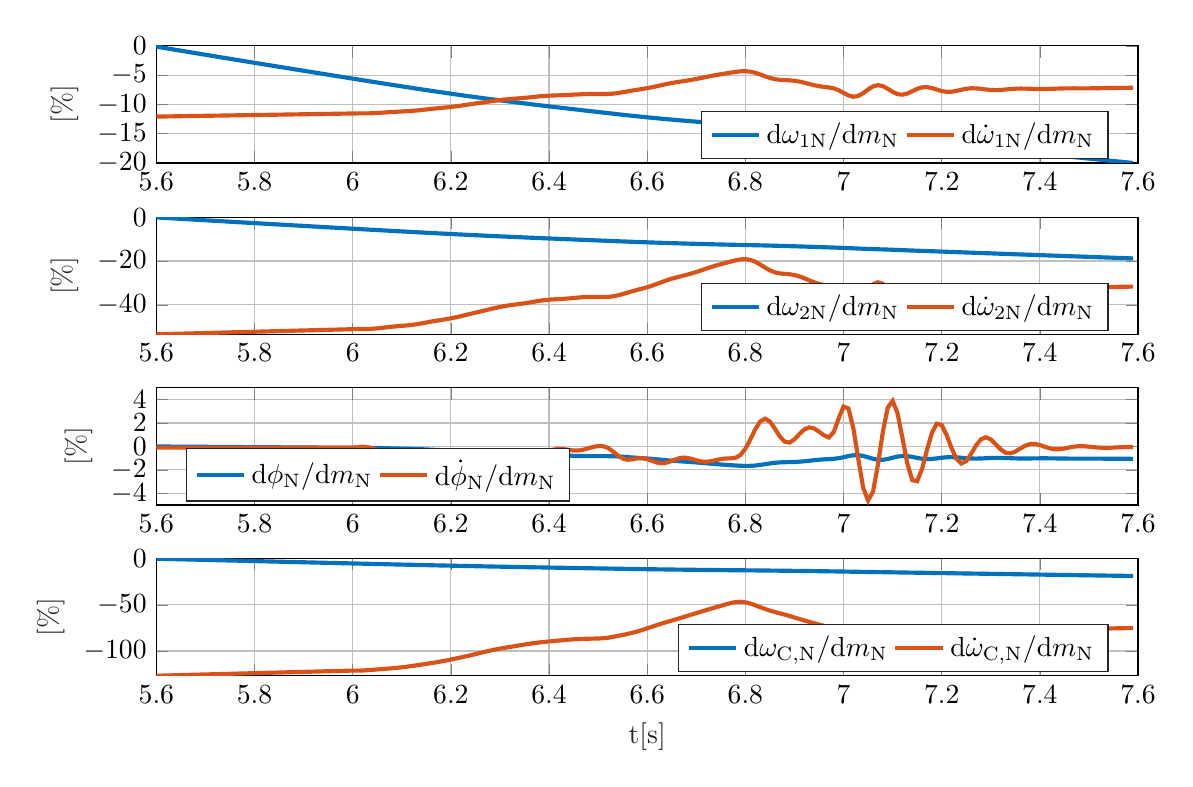
\begin{tikzpicture}

\begin{axis}[%
width=0.959\mwidth,
height=0.186\mheight,
at={(0\mwidth,0.814\mheight)},
scale only axis,
xmin=5.6,
xmax=7.6,
ymin=-20.0293942399798,
ymax=0,
ylabel style={font=\color{white!15!black}},
ylabel={[$\%$]},
axis background/.style={fill=white},
xmajorgrids,
ymajorgrids,
legend style={at={(0.97,0.03)}, anchor=south east, legend columns=2, legend cell align=left, align=left, draw=white!15!black}
]
\addplot [color=mycolor1, line width=1.5pt]
  table[row sep=crcr]{%
5.59	0\\
5.6	-0.139810221040241\\
5.61	-0.279466182537238\\
5.62	-0.4189676049814\\
5.63	-0.558314882035203\\
5.64	-0.697507734480997\\
5.65	-0.836546555773164\\
5.66	-0.975431066985564\\
5.67	-1.11416166136375\\
5.68	-1.25273806027271\\
5.69	-1.39116065674829\\
5.7	-1.52942917244599\\
5.71	-1.66754263141883\\
5.72	-1.80550346365206\\
5.73	-1.94331075321004\\
5.74	-2.08096419236808\\
5.75	-2.21846417251694\\
5.76	-2.35581041610398\\
5.77	-2.49300331541245\\
5.78	-2.63004259342155\\
5.79	-2.76692864225318\\
5.8	-2.90366118507353\\
5.81	-3.04024061361465\\
5.82	-3.1766666511766\\
5.83	-3.31293968920597\\
5.84	-3.44905945131389\\
5.85	-3.5850263288149\\
5.86	-3.72084004569546\\
5.87	-3.8565009931018\\
5.88	-3.99200889529764\\
5.89	-4.12736414315661\\
5.9	-4.262566461156\\
5.91	-4.39761623988926\\
5.92	-4.53252463452141\\
5.93	-4.66729196533479\\
5.94	-4.8019008520116\\
5.95	-4.93636320800014\\
5.96	-5.07067320832231\\
5.97	-5.20482910509364\\
5.98	-5.33882985015196\\
5.99	-5.47266730692488\\
6	-5.6063554322941\\
6.01	-5.73989630305788\\
6.02	-5.87336480887284\\
6.03	-6.00680643608757\\
6.04	-6.1400909308024\\
6.05	-6.2730208618018\\
6.06	-6.40539018884776\\
6.07	-6.53707431210649\\
6.08	-6.6680691657901\\
6.09	-6.79846240219479\\
6.1	-6.92835149710749\\
6.11	-7.05776482298917\\
6.12	-7.18662124607314\\
6.13	-7.31475414256393\\
6.14	-7.44197748128146\\
6.15	-7.56816911204738\\
6.16	-7.69329168176639\\
6.17	-7.8173848432785\\
6.18	-7.94051395246219\\
6.19	-8.06270345998733\\
6.2	-8.18390764043554\\
6.21	-8.30401531821018\\
6.22	-8.42287628265668\\
6.23	-8.54036276298309\\
6.24	-8.6564112400119\\
6.25	-8.7710246267601\\
6.26	-8.88421477035866\\
6.27	-8.99604930493717\\
6.28	-9.10650088322284\\
6.29	-9.21557199367012\\
6.3	-9.32331707979324\\
6.31	-9.42986642969375\\
6.32	-9.53540267184335\\
6.33	-9.64009772901266\\
6.34	-9.74404306529644\\
6.35	-9.84721643183919\\
6.36	-9.94951291486723\\
6.37	-10.0508268960878\\
6.38	-10.1511366542559\\
6.39	-10.2505453433746\\
6.4	-10.3492538716511\\
6.41	-10.4474801535906\\
6.42	-10.5453708970069\\
6.43	-10.6429528121929\\
6.44	-10.7401497513395\\
6.45	-10.83685435644\\
6.46	-10.9330129326722\\
6.47	-11.0286782904549\\
6.48	-11.1240030119179\\
6.49	-11.2191801314204\\
6.5	-11.3143666212183\\
6.51	-11.4096223906845\\
6.52	-11.5048369999983\\
6.53	-11.5996594132069\\
6.54	-11.6935871880734\\
6.55	-11.7861157803096\\
6.56	-11.8769653684323\\
6.57	-11.9660845758372\\
6.58	-12.0535830762377\\
6.59	-12.1395612200712\\
6.6	-12.2239812309499\\
6.61	-12.3066558340964\\
6.62	-12.3873360691942\\
6.63	-12.4658466544944\\
6.64	-12.5421898194048\\
6.65	-12.6165286550104\\
6.66	-12.6891128483074\\
6.67	-12.7601560941607\\
6.68	-12.8297459356005\\
6.69	-12.8978114471024\\
6.7	-12.9641755766412\\
6.71	-13.0286504223226\\
6.72	-13.0911307686945\\
6.73	-13.1516327170445\\
6.74	-13.2102727107401\\
6.75	-13.2672026278388\\
6.76	-13.3225243231426\\
6.77	-13.3763095879861\\
6.78	-13.4285717634385\\
6.79	-13.4794786913101\\
6.8	-13.5296358848656\\
6.81	-13.5800767905016\\
6.82	-13.6320644652319\\
6.83	-13.6868427541489\\
6.84	-13.7451611551319\\
6.85	-13.8070232273794\\
6.86	-13.8717401641417\\
6.87	-13.9382763475781\\
6.88	-14.0057122920578\\
6.89	-14.0736140081793\\
6.9	-14.1421465223472\\
6.91	-14.2119098641841\\
6.92	-14.2836047234782\\
6.93	-14.3577041404141\\
6.94	-14.4342768159538\\
6.95	-14.5130208108556\\
6.96	-14.593455376242\\
6.97	-14.6751658449661\\
6.98	-14.7582070896968\\
6.99	-14.8438847686532\\
7	-14.9340766416692\\
7.01	-15.029727132976\\
7.02	-15.1293505290626\\
7.03	-15.2294312090231\\
7.04	-15.3259093293885\\
7.05	-15.4156956428251\\
7.06	-15.4986654239158\\
7.07	-15.5771508815661\\
7.08	-15.6554056969672\\
7.09	-15.7374297330585\\
7.1	-15.8252784681969\\
7.11	-15.9186329271333\\
7.12	-16.0148804787954\\
7.13	-16.1104173263736\\
7.14	-16.2024697557177\\
7.15	-16.2895728199826\\
7.16	-16.3727903600612\\
7.17	-16.4543561571939\\
7.18	-16.5366992670832\\
7.19	-16.621583912553\\
7.2	-16.7095487067649\\
7.21	-16.7998164024244\\
7.22	-16.8907336630753\\
7.23	-16.9806474759949\\
7.24	-17.0685509681823\\
7.25	-17.1542460491764\\
7.26	-17.2384244898221\\
7.27	-17.3222882674622\\
7.28	-17.4067792872892\\
7.29	-17.492400784828\\
7.3	-17.5791552683964\\
7.31	-17.6665766443867\\
7.32	-17.753904779392\\
7.33	-17.8406047247093\\
7.34	-17.926399316022\\
7.35	-18.0113440970216\\
7.36	-18.0958156817628\\
7.37	-18.1802533141949\\
7.38	-18.2649151496489\\
7.39	-18.349924744811\\
7.4	-18.4352213720252\\
7.41	-18.5206017625856\\
7.42	-18.6058076544373\\
7.43	-18.6907060387476\\
7.44	-18.7752304550141\\
7.45	-18.8594298100492\\
7.46	-18.9434219331101\\
7.47	-19.0273582440928\\
7.48	-19.1113133998887\\
7.49	-19.1953068303513\\
7.5	-19.2792931368649\\
7.51	-19.3632172089515\\
7.52	-19.4469845859881\\
7.53	-19.530592586851\\
7.54	-19.6140231015892\\
7.55	-19.6973004822493\\
7.56	-19.7804562183098\\
7.57	-19.8635074475691\\
7.58	-19.9464861977915\\
7.59	-20.0293942399798\\
};
\addlegendentry{d$\omega_{1\mathrm{N}}/$d$m_\mathrm{N}$}

\addplot [color=mycolor2, line width=1.5pt]
  table[row sep=crcr]{%
5.59	-12.1124811943887\\
5.6	-12.0991087802569\\
5.61	-12.0857413130158\\
5.62	-12.0723787898078\\
5.63	-12.0590212170331\\
5.64	-12.0456685920522\\
5.65	-12.0323209209925\\
5.66	-12.0189782014375\\
5.67	-12.0056404392427\\
5.68	-11.9923076322089\\
5.69	-11.9789797859131\\
5.7	-11.9656568983693\\
5.71	-11.9523390918238\\
5.72	-11.9390261770626\\
5.73	-11.9257181989811\\
5.74	-11.9124151584764\\
5.75	-11.8991170729847\\
5.76	-11.8858239568845\\
5.77	-11.8725358261825\\
5.78	-11.8592526832005\\
5.79	-11.8459745279314\\
5.8	-11.8327013512959\\
5.81	-11.8194331495933\\
5.82	-11.8061699182498\\
5.83	-11.7929116616998\\
5.84	-11.7796583832767\\
5.85	-11.7664100908168\\
5.86	-11.75316678668\\
5.87	-11.7399284739728\\
5.88	-11.7266951502106\\
5.89	-11.7134668150018\\
5.9	-11.7002434654489\\
5.91	-11.6870251024983\\
5.92	-11.6738112732956\\
5.93	-11.6606012097689\\
5.94	-11.6473895780416\\
5.95	-11.6341542570397\\
5.96	-11.6208563314503\\
5.97	-11.6074677367063\\
5.98	-11.5939965670987\\
5.99	-11.58050964368\\
6	-11.5671038142836\\
6.01	-11.5558146619943\\
6.02	-11.5546346146457\\
6.03	-11.5478989501705\\
6.04	-11.5270234654163\\
6.05	-11.4864384215007\\
6.06	-11.4307968642885\\
6.07	-11.3695296773087\\
6.08	-11.3128863582261\\
6.09	-11.2655080999044\\
6.1	-11.2245760041724\\
6.11	-11.1814294747937\\
6.12	-11.1268241374327\\
6.13	-11.0558922997359\\
6.14	-10.9707267481257\\
6.15	-10.8782584343383\\
6.16	-10.7865309002363\\
6.17	-10.7003803240449\\
6.18	-10.6190509004936\\
6.19	-10.5369983363144\\
6.2	-10.4476646315601\\
6.21	-10.3461515269718\\
6.22	-10.2319761340168\\
6.23	-10.1091772470051\\
6.24	-9.9840434056902\\
6.25	-9.86119742517277\\
6.26	-9.7413756140338\\
6.27	-9.62205764397812\\
6.28	-9.50199297705124\\
6.29	-9.38366207639267\\
6.3	-9.2733437182988\\
6.31	-9.17743142249958\\
6.32	-9.09808313665155\\
6.33	-9.0308819171505\\
6.34	-8.96658462303823\\
6.35	-8.89579123170721\\
6.36	-8.81452488391471\\
6.37	-8.72676421946626\\
6.38	-8.64252377949367\\
6.39	-8.57238905686243\\
6.4	-8.52176977332806\\
6.41	-8.48800738635618\\
6.42	-8.46189203123727\\
6.43	-8.43284702652832\\
6.44	-8.39456381471141\\
6.45	-8.34822159195004\\
6.46	-8.30158286550662\\
6.47	-8.26443208629657\\
6.48	-8.24339166720902\\
6.49	-8.23849424838809\\
6.5	-8.24353433537714\\
6.51	-8.24804887881339\\
6.52	-8.23306581240375\\
6.53	-8.17855010885855\\
6.54	-8.07742768540619\\
6.55	-7.94034992417827\\
6.56	-7.78919205271163\\
6.57	-7.64306579068171\\
6.58	-7.50848843532574\\
6.59	-7.37771128870541\\
6.6	-7.23648889375236\\
6.61	-7.07435930628232\\
6.62	-6.89210210052622\\
6.63	-6.70155399015896\\
6.64	-6.51879302239248\\
6.65	-6.35568923770756\\
6.66	-6.21452056104809\\
6.67	-6.0873943536063\\
6.68	-5.96066521489115\\
6.69	-5.82188330062228\\
6.7	-5.66581832038014\\
6.71	-5.49604314222635\\
6.72	-5.32230303588875\\
6.73	-5.15502835928889\\
6.74	-5.00045315612166\\
6.75	-4.85841751496232\\
6.76	-4.72329447333795\\
6.77	-4.58941482959538\\
6.78	-4.46144563879301\\
6.79	-4.36361326409487\\
6.8	-4.33758411539042\\
6.81	-4.41370284568463\\
6.82	-4.60601053710227\\
6.83	-4.88978263763616\\
6.84	-5.20773869035621\\
6.85	-5.49283744206052\\
6.86	-5.69686137372217\\
6.87	-5.80963673433692\\
6.88	-5.86007024545239\\
6.89	-5.89937872798239\\
6.9	-5.97584811572054\\
6.91	-6.11391689423222\\
6.92	-6.30675570225711\\
6.93	-6.52414664188573\\
6.94	-6.72944265213422\\
6.95	-6.89732720099657\\
6.96	-7.02312578650035\\
6.97	-7.12222810437527\\
6.98	-7.27441908333333\\
6.99	-7.58710111884541\\
7	-8.04345147474997\\
7.01	-8.48643078060353\\
7.02	-8.70193071291363\\
7.03	-8.56583473941537\\
7.04	-8.09277085852708\\
7.05	-7.464132448144\\
7.06	-6.93510987157002\\
7.07	-6.72301334864204\\
7.08	-6.88495889465132\\
7.09	-7.3377396519963\\
7.1	-7.8673980432063\\
7.11	-8.25760047183762\\
7.12	-8.35303539535555\\
7.13	-8.15565449465661\\
7.14	-7.76388569585187\\
7.15	-7.35841421296713\\
7.16	-7.10085448694279\\
7.17	-7.05887765868716\\
7.18	-7.21962781687316\\
7.19	-7.48480646969814\\
7.2	-7.73537372128292\\
7.21	-7.87187631376626\\
7.22	-7.84968503937022\\
7.23	-7.70781780053048\\
7.24	-7.51018130203963\\
7.25	-7.33938955184085\\
7.26	-7.25753486390285\\
7.27	-7.27526378522519\\
7.28	-7.35948203499189\\
7.29	-7.46682759301753\\
7.3	-7.54983606096169\\
7.31	-7.57594099197697\\
7.32	-7.54008503348453\\
7.33	-7.46816281179191\\
7.34	-7.38774771069289\\
7.35	-7.32844184023317\\
7.36	-7.3065395931288\\
7.37	-7.31625065279818\\
7.38	-7.34391705950085\\
7.39	-7.37415889754\\
7.4	-7.39142183568378\\
7.41	-7.38815916578493\\
7.42	-7.36543390055424\\
7.43	-7.3336725985006\\
7.44	-7.30185909381554\\
7.45	-7.27836772046911\\
7.46	-7.26776131486108\\
7.47	-7.266620755261\\
7.48	-7.26986835820757\\
7.49	-7.27235990777038\\
7.5	-7.26942532677253\\
7.51	-7.26123193533613\\
7.52	-7.24748113772952\\
7.53	-7.23194760348149\\
7.54	-7.21696687331263\\
7.55	-7.20421004408459\\
7.56	-7.19417608746393\\
7.57	-7.18678095268055\\
7.58	-7.1805960661649\\
7.59	-7.1744100715263\\
};
\addlegendentry{d$\dot{\omega}_{1\mathrm{N}}/$d$m_\mathrm{N}$}

\end{axis}

\begin{axis}[%
width=0.959\mwidth,
height=0.186\mheight,
at={(0\mwidth,0.542\mheight)},
scale only axis,
xmin=5.6,
xmax=7.6,
ymin=-53.4362307924602,
ymax=0,
ylabel style={font=\color{white!15!black}},
ylabel={[$\%$]},
axis background/.style={fill=white},
xmajorgrids,
ymajorgrids,
legend style={at={(0.97,0.03)}, anchor=south east, legend columns=2, legend cell align=left, align=left, draw=white!15!black}
]
\addplot [color=mycolor1, line width=1.5pt]
  table[row sep=crcr]{%
5.59	0\\
5.6	-0.131411319107663\\
5.61	-0.262677645596664\\
5.62	-0.393798716748583\\
5.63	-0.524774902577159\\
5.64	-0.65560594063835\\
5.65	-0.786292200750328\\
5.66	-0.916833420743044\\
5.67	-1.04722997023838\\
5.68	-1.17748158733992\\
5.69	-1.30758864147245\\
5.7	-1.43755087101262\\
5.71	-1.56736735864209\\
5.72	-1.69704038836816\\
5.73	-1.82656909927873\\
5.74	-1.95595320213525\\
5.75	-2.08519306481624\\
5.76	-2.21428842644263\\
5.77	-2.34323965573181\\
5.78	-2.47204649230461\\
5.79	-2.60070930472675\\
5.8	-2.72922783279485\\
5.81	-2.85760244470818\\
5.82	-2.98583288038918\\
5.83	-3.11391950776882\\
5.84	-3.24186206706193\\
5.85	-3.36966092607535\\
5.86	-3.49731582537668\\
5.87	-3.62482713261459\\
5.88	-3.75219458861726\\
5.89	-3.87941856077715\\
5.9	-4.00649879012318\\
5.91	-4.13343564378445\\
5.92	-4.26023960679518\\
5.93	-4.38691098019719\\
5.94	-4.51343342777075\\
5.95	-4.63981814728058\\
5.96	-4.76605966367593\\
5.97	-4.892156334074\\
5.98	-5.0181071732795\\
5.99	-5.14390453351317\\
6	-5.26956153321668\\
6.01	-5.39508012442757\\
6.02	-5.52053069791191\\
6.03	-5.64595600749005\\
6.04	-5.77123362408172\\
6.05	-5.89617797687328\\
6.06	-6.02059540320363\\
6.07	-6.1443687883983\\
6.08	-6.2674943109159\\
6.09	-6.39005435746448\\
6.1	-6.51214054811049\\
6.11	-6.63377955087932\\
6.12	-6.7548951060009\\
6.13	-6.8753305993694\\
6.14	-6.99491117536564\\
6.15	-7.11352202181139\\
6.16	-7.23112802954575\\
6.17	-7.34776646931968\\
6.18	-7.4634987708495\\
6.19	-7.57834791596492\\
6.2	-7.69227092613828\\
6.21	-7.80516330449163\\
6.22	-7.91688386406288\\
6.23	-8.02731250970951\\
6.24	-8.1363895380793\\
6.25	-8.24411768719392\\
6.26	-8.35050809248479\\
6.27	-8.4556243250564\\
6.28	-8.55944068048482\\
6.29	-8.66195949773418\\
6.3	-8.7632319497016\\
6.31	-8.86338049761413\\
6.32	-8.96257679879555\\
6.33	-9.0609824479982\\
6.34	-9.15868341474041\\
6.35	-9.25565878673596\\
6.36	-9.35180995275782\\
6.37	-9.44703763938318\\
6.38	-9.54132143024034\\
6.39	-9.63475828250085\\
6.4	-9.7275370350948\\
6.41	-9.81986251162055\\
6.42	-9.9118726066268\\
6.43	-10.0035924258233\\
6.44	-10.0949503958734\\
6.45	-10.1858456081511\\
6.46	-10.276227593475\\
6.47	-10.3661459897524\\
6.48	-10.4557442129565\\
6.49	-10.5452037011801\\
6.5	-10.6346719967917\\
6.51	-10.7242054101934\\
6.52	-10.8137001360808\\
6.53	-10.9028262264916\\
6.54	-10.991111422697\\
6.55	-11.0780814901961\\
6.56	-11.1634734173868\\
6.57	-11.2472389140419\\
6.58	-11.3294810653809\\
6.59	-11.4102941934307\\
6.6	-11.4896427911663\\
6.61	-11.5673508340786\\
6.62	-11.6431843177921\\
6.63	-11.71697849036\\
6.64	-11.7887354472637\\
6.65	-11.8586084821196\\
6.66	-11.9268322823294\\
6.67	-11.9936077053405\\
6.68	-12.0590170351595\\
6.69	-12.1229936070128\\
6.7	-12.1853710050262\\
6.71	-12.2459726152463\\
6.72	-12.3046995428912\\
6.73	-12.3615669219862\\
6.74	-12.4166842007277\\
6.75	-12.4701941333131\\
6.76	-12.5221924557609\\
6.77	-12.5727466466422\\
6.78	-12.6218692455808\\
6.79	-12.6697180115266\\
6.8	-12.7168620823886\\
6.81	-12.7642728217277\\
6.82	-12.8131374101879\\
6.83	-12.8646249706215\\
6.84	-12.9194399758794\\
6.85	-12.9775857713464\\
6.86	-13.0384149293669\\
6.87	-13.1009540453823\\
6.88	-13.1643388705646\\
6.89	-13.2281614868141\\
6.9	-13.2925770068065\\
6.91	-13.3581494142308\\
6.92	-13.4255373059242\\
6.93	-13.4951853048491\\
6.94	-13.5671579848536\\
6.95	-13.6411715452704\\
6.96	-13.7167741175333\\
6.97	-13.7935759450394\\
6.98	-13.8716286040596\\
6.99	-13.9521593172359\\
7	-14.0369330406279\\
7.01	-14.1268374635122\\
7.02	-14.2204761245238\\
7.03	-14.3145445987239\\
7.04	-14.4052269320168\\
7.05	-14.4896194592493\\
7.06	-14.5676049477044\\
7.07	-14.6413755021287\\
7.08	-14.7149292698135\\
7.09	-14.7920258275688\\
7.1	-14.8745971737895\\
7.11	-14.9623434952111\\
7.12	-15.052809110893\\
7.13	-15.1426067170353\\
7.14	-15.2291292264566\\
7.15	-15.3109996969287\\
7.16	-15.3892180606023\\
7.17	-15.4658839074588\\
7.18	-15.5432803711032\\
7.19	-15.6230656911623\\
7.2	-15.7057461243696\\
7.21	-15.7905911154649\\
7.22	-15.8760466498535\\
7.23	-15.9605590172173\\
7.24	-16.0431818310317\\
7.25	-16.1237289008431\\
7.26	-16.2028504403364\\
7.27	-16.2816762197611\\
7.28	-16.3610915606826\\
7.29	-16.441569467461\\
7.3	-16.5231122977302\\
7.31	-16.6052819577995\\
7.32	-16.6873639782056\\
7.33	-16.7688555465325\\
7.34	-16.8494961487199\\
7.35	-16.9293379917513\\
7.36	-17.0087350651217\\
7.37	-17.0881002258195\\
7.38	-17.1676761208601\\
7.39	-17.2475788844344\\
7.4	-17.327751437015\\
7.41	-17.4080027209767\\
7.42	-17.4880899889946\\
7.43	-17.5678882225521\\
7.44	-17.6473349536691\\
7.45	-17.72647615115\\
7.46	-17.8054225658254\\
7.47	-17.8843165212544\\
7.48	-17.963228189421\\
7.49	-18.0421758329577\\
7.5	-18.1211167805077\\
7.51	-18.1999992322751\\
7.52	-18.2787344022266\\
7.53	-18.3573197703038\\
7.54	-18.4357383144847\\
7.55	-18.5140129239012\\
7.56	-18.5921731963459\\
7.57	-18.6702352400883\\
7.58	-18.7482291588698\\
7.59	-18.8261566173028\\
};
\addlegendentry{d$\omega_{2\mathrm{N}}/$d$m_\mathrm{N}$}

\addplot [color=mycolor2, line width=1.5pt]
  table[row sep=crcr]{%
5.59	-53.4952906307324\\
5.6	-53.4362307924602\\
5.61	-53.3771928023428\\
5.62	-53.3181766477581\\
5.63	-53.2591823569729\\
5.64	-53.2002099183316\\
5.65	-53.1412593588943\\
5.66	-53.0823306679888\\
5.67	-53.0234238714769\\
5.68	-52.9645389596448\\
5.69	-52.9056759571248\\
5.7	-52.8468348551433\\
5.71	-52.7880161936103\\
5.72	-52.7292191368498\\
5.73	-52.670443883145\\
5.74	-52.6116904364612\\
5.75	-52.5529588738034\\
5.76	-52.4942492586753\\
5.77	-52.4355616617712\\
5.78	-52.3768960933458\\
5.79	-52.3182525533676\\
5.8	-52.259631001737\\
5.81	-52.2010314221113\\
5.82	-52.1424537942865\\
5.83	-52.0838981378525\\
5.84	-52.0253644675259\\
5.85	-51.9668528179212\\
5.86	-51.9083631994562\\
5.87	-51.8498956258552\\
5.88	-51.7914500861421\\
5.89	-51.7330265785883\\
5.9	-51.6746250903965\\
5.91	-51.6162456257477\\
5.92	-51.5578861845897\\
5.93	-51.4995433747002\\
5.94	-51.4411936387861\\
5.95	-51.3827392781783\\
5.96	-51.3240084217354\\
5.97	-51.2648771210983\\
5.98	-51.2053811250486\\
5.99	-51.1458155516189\\
6	-51.0866081334037\\
6.01	-51.0367491100542\\
6.02	-51.0315373805289\\
6.03	-51.0017890306315\\
6.04	-50.9095915604298\\
6.05	-50.730345980216\\
6.06	-50.4846026658236\\
6.07	-50.2140135172409\\
6.08	-49.9638458787551\\
6.09	-49.7545977769149\\
6.1	-49.5738194275278\\
6.11	-49.3832609373402\\
6.12	-49.1420941321882\\
6.13	-48.8288206408474\\
6.14	-48.4526833439557\\
6.15	-48.0442930859398\\
6.16	-47.6391745130496\\
6.17	-47.258686813015\\
6.18	-46.8994919395723\\
6.19	-46.5371032846533\\
6.2	-46.1425571613397\\
6.21	-45.6942201983652\\
6.22	-45.1899596978955\\
6.23	-44.6476131675368\\
6.24	-44.0949542117492\\
6.25	-43.5523996909102\\
6.26	-43.0232015433208\\
6.27	-42.4962286314002\\
6.28	-41.965957900849\\
6.29	-41.4433444230869\\
6.3	-40.9561186818505\\
6.31	-40.532517930156\\
6.32	-40.1820728360109\\
6.33	-39.8852757793012\\
6.34	-39.601304033124\\
6.35	-39.2886419960727\\
6.36	-38.9297256994126\\
6.37	-38.5421269758088\\
6.38	-38.1700754739847\\
6.39	-37.8603224753824\\
6.4	-37.6367602472366\\
6.41	-37.4876472228734\\
6.42	-37.3723076413629\\
6.43	-37.2440291372857\\
6.44	-37.0749496968678\\
6.45	-36.870277290338\\
6.46	-36.6642953626309\\
6.47	-36.5002173591978\\
6.48	-36.4072914494679\\
6.49	-36.3856617900309\\
6.5	-36.4079215495266\\
6.51	-36.4278602234711\\
6.52	-36.3616868706081\\
6.53	-36.1209159370324\\
6.54	-35.6743044339835\\
6.55	-35.0688946456665\\
6.56	-34.4012994489881\\
6.57	-33.7559265703328\\
6.58	-33.1615599313641\\
6.59	-32.5839770766187\\
6.6	-31.9602623363978\\
6.61	-31.2442100872872\\
6.62	-30.4392633521806\\
6.63	-29.5976994826771\\
6.64	-28.7905278611315\\
6.65	-28.0701730284044\\
6.66	-27.4466955373224\\
6.67	-26.8852372114237\\
6.68	-26.3255325565184\\
6.69	-25.7125963034954\\
6.7	-25.0233286512818\\
6.71	-24.2735093243027\\
6.72	-23.5061787226215\\
6.73	-22.7674029675751\\
6.74	-22.0847149794554\\
6.75	-21.4574085026235\\
6.76	-20.860631816939\\
6.77	-20.2693466511168\\
6.78	-19.7041652531943\\
6.79	-19.2720843910175\\
6.8	-19.1571255438197\\
6.81	-19.4933071678966\\
6.82	-20.3426423022764\\
6.83	-21.5959339068062\\
6.84	-23.0002003964779\\
6.85	-24.2593512125757\\
6.86	-25.1604316225023\\
6.87	-25.6585088203322\\
6.88	-25.881250576654\\
6.89	-26.0548581689751\\
6.9	-26.3925884866341\\
6.91	-27.0023751451206\\
6.92	-27.8540559786847\\
6.93	-28.8141723503253\\
6.94	-29.7208709496728\\
6.95	-30.4623402316203\\
6.96	-31.0179350585145\\
6.97	-31.4556246789823\\
6.98	-32.1277826390309\\
6.99	-33.5087562064006\\
7	-35.5242470481833\\
7.01	-37.4806840762154\\
7.02	-38.4324487332513\\
7.03	-37.8313750523821\\
7.04	-35.7420682135205\\
7.05	-32.9656598191237\\
7.06	-30.6292090102537\\
7.07	-29.6924756561448\\
7.08	-30.4077150782815\\
7.09	-32.407440635535\\
7.1	-34.7466995469062\\
7.11	-36.4700452420991\\
7.12	-36.8915376587209\\
7.13	-36.0197964788271\\
7.14	-34.2895328428485\\
7.15	-32.4987507172641\\
7.16	-31.361227184528\\
7.17	-31.1758347293196\\
7.18	-31.8857946700688\\
7.19	-33.0569675184947\\
7.2	-34.163608489156\\
7.21	-34.7664780201423\\
7.22	-34.6684693087791\\
7.23	-34.0419065879846\\
7.24	-33.1690365495241\\
7.25	-32.4147274886804\\
7.26	-32.0532127626349\\
7.27	-32.1315133010203\\
7.28	-32.503466798854\\
7.29	-32.977563041592\\
7.3	-33.3441734863231\\
7.31	-33.4594670293347\\
7.32	-33.3011076569145\\
7.33	-32.9834600923481\\
7.34	-32.6283033630734\\
7.35	-32.3663764526886\\
7.36	-32.2696442427053\\
7.37	-32.3125335525838\\
7.38	-32.434723419673\\
7.39	-32.5682877892806\\
7.4	-32.6445302930528\\
7.41	-32.6301205720649\\
7.42	-32.5297534673688\\
7.43	-32.3894783200306\\
7.44	-32.2489726175418\\
7.45	-32.1452219636227\\
7.46	-32.0983783201575\\
7.47	-32.093340989961\\
7.48	-32.1076841671089\\
7.49	-32.1186882021906\\
7.5	-32.10572749985\\
7.51	-32.0695410365565\\
7.52	-32.0088100515041\\
7.53	-31.9402055339165\\
7.54	-31.8740424991612\\
7.55	-31.817701417914\\
7.56	-31.7733860198553\\
7.57	-31.7407250911698\\
7.58	-31.7134092756598\\
7.59	-31.6860885660772\\
};
\addlegendentry{d$\dot{\omega}_{2\mathrm{N}}/$d$m_\mathrm{N}$}

\end{axis}

\begin{axis}[%
width=0.959\mwidth,
height=0.186\mheight,
at={(0\mwidth,0.271\mheight)},
scale only axis,
xmin=5.6,
xmax=7.6,
ymin=-5,
ymax=5,
ylabel style={font=\color{white!15!black}},
ylabel={[$\%$]},
axis background/.style={fill=white},
xmajorgrids,
ymajorgrids,
legend style={at={(0.03,0.03)}, anchor=south west, legend columns=2, legend cell align=left, align=left, draw=white!15!black}
]
\addplot [color=mycolor1, line width=1.5pt]
  table[row sep=crcr]{%
5.59	0\\
5.6	-0.00286146793284332\\
5.61	-0.0057218785906564\\
5.62	-0.0085812308294148\\
5.63	-0.0114395250171215\\
5.64	-0.0142967599923561\\
5.65	-0.0171529361531348\\
5.66	-0.0200080523192472\\
5.67	-0.0228621089181435\\
5.68	-0.0257151047514039\\
5.69	-0.0285670402770578\\
5.7	-0.0314179142796295\\
5.71	-0.0342677080981643\\
5.72	-0.0371164478720934\\
5.73	-0.0399641306458333\\
5.74	-0.0428107563346126\\
5.75	-0.0456563240053936\\
5.76	-0.0485008294794828\\
5.77	-0.0513442705473622\\
5.78	-0.0541866444171547\\
5.79	-0.0570279518089542\\
5.8	-0.0598681927004518\\
5.81	-0.0627073693535062\\
5.82	-0.065545481611699\\
5.83	-0.0683825304407881\\
5.84	-0.0712185140242454\\
5.85	-0.0740534322083354\\
5.86	-0.0768872829267499\\
5.87	-0.079720066652441\\
5.88	-0.0825517822797516\\
5.89	-0.0853824311535057\\
5.9	-0.0882120125388774\\
5.91	-0.0910405276984191\\
5.92	-0.0938680608201499\\
5.93	-0.0966947003910457\\
5.94	-0.099520984955443\\
5.95	-0.102349911778202\\
5.96	-0.105188232740947\\
5.97	-0.108043076230577\\
5.98	-0.11091672512147\\
5.99	-0.113800985577384\\
6	-0.116677617518482\\
6.01	-0.119386756193221\\
6.02	-0.12059724714536\\
6.03	-0.121386308198269\\
6.04	-0.124397937010322\\
6.05	-0.131039232175855\\
6.06	-0.141389563372803\\
6.07	-0.153920829886177\\
6.08	-0.166509941023825\\
6.09	-0.177576591266087\\
6.1	-0.186959418866935\\
6.11	-0.195923218028608\\
6.12	-0.20639851464883\\
6.13	-0.21988043338065\\
6.14	-0.23662399082954\\
6.15	-0.255649125918033\\
6.16	-0.275343978005934\\
6.17	-0.294340323793514\\
6.18	-0.312219669600708\\
6.19	-0.329691014706889\\
6.2	-0.348014285314125\\
6.21	-0.368439790171046\\
6.22	-0.391548207218386\\
6.23	-0.416939198570604\\
6.24	-0.443461601737538\\
6.25	-0.469962070229096\\
6.26	-0.495880109199842\\
6.27	-0.521462884571269\\
6.28	-0.547088047575066\\
6.29	-0.572620974571811\\
6.3	-0.597094143694272\\
6.31	-0.619140868112106\\
6.32	-0.637845506651963\\
6.33	-0.65347433748101\\
6.34	-0.667508486234798\\
6.35	-0.681976774429149\\
6.36	-0.698303340696417\\
6.37	-0.71645359923184\\
6.38	-0.734890655552718\\
6.39	-0.751390590331763\\
6.4	-0.764248568472717\\
6.41	-0.773203516663425\\
6.42	-0.779565367768269\\
6.43	-0.785472029125549\\
6.44	-0.792726079645437\\
6.45	-0.801846742356471\\
6.46	-0.811838729843664\\
6.47	-0.820803470700482\\
6.48	-0.826986224006449\\
6.49	-0.829699054539344\\
6.5	-0.829633314104965\\
6.51	-0.828554930179113\\
6.52	-0.829626759429315\\
6.53	-0.837133036653277\\
6.54	-0.853909814385506\\
6.55	-0.879537497251952\\
6.56	-0.91039605608937\\
6.57	-0.942124939807763\\
6.58	-0.972018543631572\\
6.59	-1.00030750923339\\
6.6	-1.02939073406493\\
6.61	-1.0619128394598\\
6.62	-1.09884711033658\\
6.63	-1.13878915792536\\
6.64	-1.17871499973612\\
6.65	-1.2156646557946\\
6.66	-1.24813483792307\\
6.67	-1.27676434220466\\
6.68	-1.30389149034049\\
6.69	-1.33233291269491\\
6.7	-1.36394669513411\\
6.71	-1.39887766157\\
6.72	-1.43565438619283\\
6.73	-1.47211621351964\\
6.74	-1.50649670787156\\
6.75	-1.53816826568036\\
6.76	-1.56778299280047\\
6.77	-1.59660599782591\\
6.78	-1.62473507445227\\
6.79	-1.64900112488297\\
6.8	-1.66208496848649\\
6.81	-1.65685421828439\\
6.82	-1.62790034386317\\
6.83	-1.57664642747573\\
6.84	-1.51207985261778\\
6.85	-1.44762072682735\\
6.86	-1.39557103485267\\
6.87	-1.36204572904038\\
6.88	-1.34487178072804\\
6.89	-1.33535506584755\\
6.9	-1.32283760596369\\
6.91	-1.29962544566625\\
6.92	-1.26397259447824\\
6.93	-1.21994810130977\\
6.94	-1.17476883665345\\
6.95	-1.13500351311844\\
6.96	-1.10377613719473\\
6.97	-1.07992124776934\\
6.98	-1.05381410434275\\
6.99	-1.00340363283719\\
7	-0.919978071542453\\
7.01	-0.822898570601033\\
7.02	-0.753031320061849\\
7.03	-0.745131460633252\\
7.04	-0.811743560396915\\
7.05	-0.930790041754404\\
7.06	-1.05453176249474\\
7.07	-1.13236245251202\\
7.08	-1.13705378353496\\
7.09	-1.06962406296942\\
7.1	-0.964537238207107\\
7.11	-0.866171507312591\\
7.12	-0.815837797965909\\
7.13	-0.827205475522697\\
7.14	-0.891178213035544\\
7.15	-0.976718155690205\\
7.16	-1.04663826308602\\
7.17	-1.07825782712075\\
7.18	-1.06458193459154\\
7.19	-1.01888881208116\\
7.2	-0.963643258714691\\
7.21	-0.922551921434153\\
7.22	-0.911474326553596\\
7.23	-0.928919072805694\\
7.24	-0.965573746713511\\
7.25	-1.00496669813622\\
7.26	-1.03130963839825\\
7.27	-1.03754761151124\\
7.28	-1.02687655982645\\
7.29	-1.00638366681007\\
7.3	-0.98605355146172\\
7.31	-0.974633223820359\\
7.32	-0.976233060861402\\
7.33	-0.987573816989756\\
7.34	-1.0039096044867\\
7.35	-1.01872300656207\\
7.36	-1.02702675293717\\
7.37	-1.02831420726467\\
7.38	-1.02446934010551\\
7.39	-1.01824787875881\\
7.4	-1.01321156552561\\
7.41	-1.01179023611894\\
7.42	-1.01476856592994\\
7.43	-1.02050436693304\\
7.44	-1.02731504266591\\
7.45	-1.03320861442056\\
7.46	-1.03670005700194\\
7.47	-1.03795837298956\\
7.48	-1.03778928686617\\
7.49	-1.03717989176756\\
7.5	-1.03730908239439\\
7.51	-1.03844739596729\\
7.52	-1.04089830557542\\
7.53	-1.04397368597238\\
7.54	-1.0472058908743\\
7.55	-1.05015344224505\\
7.56	-1.05259710891306\\
7.57	-1.05443950702118\\
7.58	-1.05590682077998\\
7.59	-1.05723271786267\\
};
\addlegendentry{d$\phi_\mathrm{N}/$d$m_\mathrm{N}$}

\addplot [color=mycolor2, line width=1.5pt]
  table[row sep=crcr]{%
5.59	-0.101443326784142\\
5.6	-0.101405880970175\\
5.61	-0.101368358631607\\
5.62	-0.101330884199888\\
5.63	-0.101293334526713\\
5.64	-0.101255831967856\\
5.65	-0.10121825538639\\
5.66	-0.101180725088973\\
5.67	-0.101143121973816\\
5.68	-0.101105564344587\\
5.69	-0.101067935152807\\
5.7	-0.10103035068238\\
5.71	-0.100992279787047\\
5.72	-0.100954739100075\\
5.73	-0.100917257261622\\
5.74	-0.100879826672065\\
5.75	-0.100842249042278\\
5.76	-0.100804602529448\\
5.77	-0.100766801000767\\
5.78	-0.10072900715278\\
5.79	-0.100691170046897\\
5.8	-0.100653428957387\\
5.81	-0.100615679674204\\
5.82	-0.100578002652452\\
5.83	-0.100540262173763\\
5.84	-0.100502536465212\\
5.85	-0.100464717569354\\
5.86	-0.100426916181847\\
5.87	-0.100389051653297\\
5.88	-0.100351240045364\\
5.89	-0.100313391967059\\
5.9	-0.10027560345153\\
5.91	-0.100237770640965\\
5.92	-0.100200793596788\\
5.93	-0.100170048075772\\
5.94	-0.100188250099556\\
5.95	-0.10037841438572\\
5.96	-0.100852100480422\\
5.97	-0.101529621529495\\
5.98	-0.102126399776322\\
5.99	-0.10220988390872\\
6	-0.101604286025514\\
6.01	-0.0807710113182941\\
6.02	-0.0128604531182624\\
6.03	-0.0590772796329837\\
6.04	-0.162183749088303\\
6.05	-0.306904697277795\\
6.06	-0.417047942705917\\
6.07	-0.45790960141509\\
6.08	-0.424547399275582\\
6.09	-0.358596323463667\\
6.1	-0.314244771284313\\
6.11	-0.333179490470105\\
6.12	-0.418749617752895\\
6.13	-0.538793269472743\\
6.14	-0.643495132039095\\
6.15	-0.697215930667589\\
6.16	-0.692228969995163\\
6.17	-0.652178558251977\\
6.18	-0.618192158925556\\
6.19	-0.624094042573633\\
6.2	-0.680029000630994\\
6.21	-0.771652685667824\\
6.22	-0.865126544778546\\
6.23	-0.927578315407856\\
6.24	-0.945239914860986\\
6.25	-0.929759704922162\\
6.26	-0.909702289236876\\
6.27	-0.905769276510274\\
6.28	-0.91015565083478\\
6.29	-0.8947867303025\\
6.3	-0.833024987136905\\
6.31	-0.724787875797689\\
6.32	-0.602254895085217\\
6.33	-0.513536080415186\\
6.34	-0.493817962752119\\
6.35	-0.541842406465328\\
6.36	-0.616969455308915\\
6.37	-0.661312492401575\\
6.38	-0.631939498741612\\
6.39	-0.525959967218049\\
6.4	-0.382181101138325\\
6.41	-0.259427551016726\\
6.42	-0.204516332508652\\
6.43	-0.226301351690097\\
6.44	-0.292678094740875\\
6.45	-0.348957861680581\\
6.46	-0.347969712292177\\
6.47	-0.27590883184599\\
6.48	-0.156728910567462\\
6.49	-0.0386997843253404\\
6.5	0.033075841525183\\
6.51	0.0250992620930155\\
6.52	-0.126149696739947\\
6.53	-0.420821806074558\\
6.54	-0.765163554162212\\
6.55	-1.02738423214513\\
6.56	-1.13234267006497\\
6.57	-1.09930030603854\\
6.58	-1.02120771615422\\
6.59	-0.999228943156152\\
6.6	-1.0793563978662\\
6.61	-1.23278510361685\\
6.62	-1.37870030436244\\
6.63	-1.4371429589171\\
6.64	-1.37863807541181\\
6.65	-1.23299052714719\\
6.66	-1.07221612200297\\
6.67	-0.970729491422061\\
6.68	-0.969716819218728\\
6.69	-1.05832772781083\\
6.7	-1.18417053495426\\
6.71	-1.28279477320448\\
6.72	-1.31071127286922\\
6.73	-1.26289772502838\\
6.74	-1.17002664455673\\
6.75	-1.07901135987271\\
6.76	-1.02896280164524\\
6.77	-1.01617928864586\\
6.78	-0.962950180942568\\
6.79	-0.726513411849274\\
6.8	-0.193800980354092\\
6.81	0.589795466859987\\
6.82	1.45382862886252\\
6.83	2.12421341506566\\
6.84	2.36933812087562\\
6.85	2.12378041067775\\
6.86	1.52833119052998\\
6.87	0.862163250410252\\
6.88	0.409626026199164\\
6.89	0.33116077989287\\
6.9	0.603550862883502\\
6.91	1.05202712298896\\
6.92	1.44925260360601\\
6.93	1.62539407903456\\
6.94	1.53625239676061\\
6.95	1.2635169109959\\
6.96	0.957743942971941\\
6.97	0.769712038760238\\
6.98	1.22714602298062\\
6.99	2.39575413208685\\
7	3.4028700893264\\
7.01	3.23933622842062\\
7.02	1.55491489478125\\
7.03	-1.06904323723583\\
7.04	-3.52146473237528\\
7.05	-4.61640616067641\\
7.06	-3.86779289598544\\
7.07	-1.56726217535532\\
7.08	1.22127981482951\\
7.09	3.30813888479361\\
7.1	3.89153540561606\\
7.11	2.83643574849915\\
7.12	0.715813343869345\\
7.13	-1.47176953610082\\
7.14	-2.87839974461504\\
7.15	-2.96403000396846\\
7.16	-1.91372175895609\\
7.17	-0.30894520074833\\
7.18	1.15949266028134\\
7.19	1.94207893925872\\
7.2	1.82594354236397\\
7.21	0.98328788835546\\
7.22	-0.138499208817952\\
7.23	-1.05340899140323\\
7.24	-1.45237907559185\\
7.25	-1.25012879272186\\
7.26	-0.624159615623335\\
7.27	0.0868929625919987\\
7.28	0.607682927740573\\
7.29	0.782982111016209\\
7.3	0.600734572495915\\
7.31	0.187091088478689\\
7.32	-0.243278494394545\\
7.33	-0.530119897225139\\
7.34	-0.591683667802546\\
7.35	-0.44102986844043\\
7.36	-0.184571742937772\\
7.37	0.0539640501513128\\
7.38	0.200993813037347\\
7.39	0.21861461702554\\
7.4	0.123413447717768\\
7.41	-0.0268188128775158\\
7.42	-0.160338646446538\\
7.43	-0.235429381487578\\
7.44	-0.23511843829427\\
7.45	-0.173607452373278\\
7.46	-0.0869657072902995\\
7.47	-0.0150661795690906\\
7.48	0.0221996982630862\\
7.49	0.0167879550853782\\
7.5	-0.0185587972091163\\
7.51	-0.0621258085032327\\
7.52	-0.0969295131530281\\
7.53	-0.114503284655732\\
7.54	-0.112576847269863\\
7.55	-0.0971016243020796\\
7.56	-0.0760508141133183\\
7.57	-0.0576022258766949\\
7.58	-0.047387713274649\\
7.59	-0.0472144408017388\\
};
\addlegendentry{d$\dot{\phi}_\mathrm{N}/$d$m_\mathrm{N}$}

\end{axis}

\begin{axis}[%
width=0.959\mwidth,
height=0.186\mheight,
at={(0\mwidth,0\mheight)},
scale only axis,
xmin=5.6,
xmax=7.6,
xlabel style={font=\color{white!15!black}},
xlabel={t[s]},
ymin=-126.697507996823,
ymax=0,
ylabel style={font=\color{white!15!black}},
ylabel={[$\%$]},
axis background/.style={fill=white},
xmajorgrids,
ymajorgrids,
legend style={at={(0.97,0.03)}, anchor=south east, legend columns=2, legend cell align=left, align=left, draw=white!15!black}
]
\addplot [color=mycolor1, line width=1.5pt]
  table[row sep=crcr]{%
5.59	0\\
5.6	-0.131411962234403\\
5.61	-0.262678931481211\\
5.62	-0.393800644661217\\
5.63	-0.524777472145666\\
5.64	-0.655609151135747\\
5.65	-0.786296051801315\\
5.66	-0.916837911623472\\
5.67	-1.0472351005699\\
5.68	-1.17748735640114\\
5.69	-1.30759504888183\\
5.7	-1.4375579160514\\
5.71	-1.56737504212322\\
5.72	-1.69704870817501\\
5.73	-1.82657805465376\\
5.74	-1.95596279234172\\
5.75	-2.08520328969212\\
5.76	-2.21429928559889\\
5.77	-2.34325114902991\\
5.78	-2.47205861913463\\
5.79	-2.60072206462753\\
5.8	-2.72924122490155\\
5.81	-2.85761646845871\\
5.82	-2.98584753498782\\
5.83	-3.11393479281366\\
5.84	-3.24187798192389\\
5.85	-3.36967747043891\\
5.86	-3.49733299860528\\
5.87	-3.62484493430629\\
5.88	-3.75221301803358\\
5.89	-3.87943761743949\\
5.9	-4.0065184732743\\
5.91	-4.13345595296881\\
5.92	-4.26026053899802\\
5.93	-4.38693251686471\\
5.94	-4.51345542679887\\
5.95	-4.63984011099893\\
5.96	-4.7660807718947\\
5.97	-4.89217599695605\\
5.98	-5.01812562364313\\
5.99	-5.1439232545681\\
6	-5.26958251639496\\
6.01	-5.395161843483\\
6.02	-5.52080924392551\\
6.03	-5.64610146007466\\
6.04	-5.77108152563735\\
6.05	-5.89560802660184\\
6.06	-6.0197075564382\\
6.07	-6.14336332223866\\
6.08	-6.26658578960869\\
6.09	-6.38933698686413\\
6.1	-6.51155188622627\\
6.11	-6.63313664747166\\
6.12	-6.75400532881071\\
6.13	-6.8740942893103\\
6.14	-6.99337267911497\\
6.15	-7.11182871185726\\
6.16	-7.22944961462117\\
6.17	-7.34620430716902\\
6.18	-7.46203532789278\\
6.19	-7.57686787926525\\
6.2	-7.69062965594603\\
6.21	-7.80325762737706\\
6.22	-7.91470842675953\\
6.23	-8.02495698584084\\
6.24	-8.1339834019006\\
6.25	-8.2417567398016\\
6.26	-8.34820556025398\\
6.27	-8.45333359025804\\
6.28	-8.55713768808272\\
6.29	-8.65970135119889\\
6.3	-8.76115275667348\\
6.31	-8.8616146048552\\
6.32	-8.96116552903442\\
6.33	-9.05982804777645\\
6.34	-9.15758641346667\\
6.35	-9.25442335076151\\
6.36	-9.35035773031738\\
6.37	-9.44545761736585\\
6.38	-9.53982670364888\\
6.39	-9.63357030263189\\
6.4	-9.72676506986446\\
6.41	-9.81944577904564\\
6.42	-9.91161498631172\\
6.43	-10.0032722025378\\
6.44	-10.0944386620607\\
6.45	-10.1851715503407\\
6.46	-10.2755567600922\\
6.47	-10.3656838364847\\
6.48	-10.455626950571\\
6.49	-10.5454280023855\\
6.5	-10.6351041516641\\
6.51	-10.7246148707354\\
6.52	-10.8136727292852\\
6.53	-10.9019473421583\\
6.54	-10.9892374720457\\
6.55	-11.0754498640682\\
6.56	-11.1605387242008\\
6.57	-11.2444000809124\\
6.58	-11.3268683176324\\
6.59	-11.4077453110114\\
6.6	-11.48686259868\\
6.61	-11.5641274250516\\
6.62	-11.6395394046899\\
6.63	-11.713164931163\\
6.64	-11.7850913064843\\
6.65	-11.8553856647468\\
6.66	-11.9240745104797\\
6.67	-11.9911435835832\\
6.68	-12.0565561070754\\
6.69	-12.1202767822627\\
6.7	-12.1822906468545\\
6.71	-12.2426074000645\\
6.72	-12.3012538655204\\
6.73	-12.3582596958366\\
6.74	-12.4136456713232\\
6.75	-12.4674189293632\\
6.76	-12.5195621441984\\
6.77	-12.5701534955219\\
6.78	-12.6194301694987\\
6.79	-12.667962623355\\
6.8	-12.7166468551262\\
6.81	-12.7663230138204\\
6.82	-12.8176855546008\\
6.83	-12.8711112778798\\
6.84	-12.926635114554\\
6.85	-12.9840712866521\\
6.86	-13.0431793632718\\
6.87	-13.1037929706496\\
6.88	-13.1658698558837\\
6.89	-13.2294659039958\\
6.9	-13.2946691134343\\
6.91	-13.3615382462312\\
6.92	-13.4300747145558\\
6.93	-13.5002321880407\\
6.94	-13.5719474695609\\
6.95	-13.6451729054811\\
6.96	-13.7198918547179\\
6.97	-13.7961504308137\\
6.98	-13.8755257610592\\
6.99	-13.9594350229455\\
7	-14.0471204696155\\
7.01	-14.1365525135445\\
7.02	-14.2253222180919\\
7.03	-14.3118057176804\\
7.04	-14.3953989419527\\
7.05	-14.476626547939\\
7.06	-14.5567764505546\\
7.07	-14.6371976963958\\
7.08	-14.7188129011876\\
7.09	-14.8019424803159\\
7.1	-14.8862006495827\\
7.11	-14.9708972382945\\
7.12	-15.0552329113283\\
7.13	-15.1387070022682\\
7.14	-15.2211635668913\\
7.15	-15.302786830013\\
7.16	-15.3840417508663\\
7.17	-15.4653470096669\\
7.18	-15.5469887593193\\
7.19	-15.6290367103047\\
7.2	-15.711381754982\\
7.21	-15.7937911362474\\
7.22	-15.8760041480592\\
7.23	-15.957872031472\\
7.24	-16.0393418359247\\
7.25	-16.1204739001909\\
7.26	-16.201405318037\\
7.27	-16.2822869343333\\
7.28	-16.363208101963\\
7.29	-16.4441930924775\\
7.3	-16.5252094121205\\
7.31	-16.6061836430112\\
7.32	-16.6870218819524\\
7.33	-16.7676845787311\\
7.34	-16.8481475401452\\
7.35	-16.9284252192665\\
7.36	-17.0085639868416\\
7.37	-17.0886190316037\\
7.38	-17.1686202852604\\
7.39	-17.2485743124096\\
7.4	-17.3284719830718\\
7.41	-17.4082893011515\\
7.42	-17.487990915027\\
7.43	-17.5675724005341\\
7.44	-17.6470203538967\\
7.45	-17.726339689914\\
7.46	-17.8055368905166\\
7.47	-17.8846390147487\\
7.48	-17.9636587325803\\
7.49	-18.0425910531473\\
7.5	-18.1214301413557\\
7.51	-18.2001869703579\\
7.52	-18.2788218499762\\
7.53	-18.3573567355281\\
7.54	-18.4357811678521\\
7.55	-18.5141008317551\\
7.56	-18.5923222761695\\
7.57	-18.6704379689594\\
7.58	-18.7484617333846\\
7.59	-18.8263900098999\\
};
\addlegendentry{d$\omega_{\mathrm{C,N}}/$d$m_\mathrm{N}$}

\addplot [color=mycolor2, line width=1.5pt]
  table[row sep=crcr]{%
5.59	-126.837538836586\\
5.6	-126.697507996823\\
5.61	-126.557528756853\\
5.62	-126.417601489718\\
5.63	-126.277725860906\\
5.64	-126.137902243074\\
5.65	-125.99813030151\\
5.66	-125.85841040846\\
5.67	-125.718742228985\\
5.68	-125.579126134901\\
5.69	-125.439561791042\\
5.7	-125.300049568815\\
5.71	-125.160590491239\\
5.72	-125.021182182337\\
5.73	-124.881825659716\\
5.74	-124.742521347669\\
5.75	-124.60326892817\\
5.76	-124.464068769593\\
5.77	-124.324920517504\\
5.78	-124.185824516483\\
5.79	-124.046780411611\\
5.8	-123.907788566972\\
5.81	-123.768848656628\\
5.82	-123.629961064806\\
5.83	-123.491125470185\\
5.84	-123.352342243592\\
5.85	-123.213611043527\\
5.86	-123.07493222149\\
5.87	-122.936305428928\\
5.88	-122.797731018104\\
5.89	-122.659208650717\\
5.9	-122.520738682221\\
5.91	-122.382320776306\\
5.92	-122.243942111034\\
5.93	-122.105578027843\\
5.94	-121.96695910382\\
5.95	-121.827661141561\\
5.96	-121.687617723121\\
5.97	-121.547165425783\\
5.98	-121.406882123165\\
5.99	-121.267475212082\\
6	-121.129064023838\\
6.01	-121.17173852751\\
6.02	-121.045708169633\\
6.03	-120.704154743391\\
6.04	-120.335547675269\\
6.05	-119.898146153493\\
6.06	-119.478006008737\\
6.07	-119.057344938892\\
6.08	-118.627762897856\\
6.09	-118.147244568863\\
6.1	-117.586096810883\\
6.11	-116.934594581155\\
6.12	-116.207681725327\\
6.13	-115.436510840688\\
6.14	-114.647542990535\\
6.15	-113.850176888353\\
6.16	-113.034003600109\\
6.17	-112.175440800879\\
6.18	-111.251526696821\\
6.19	-110.252402329275\\
6.2	-109.184549058863\\
6.21	-108.065569111554\\
6.22	-106.916163000381\\
6.23	-105.747875847033\\
6.24	-104.556797428186\\
6.25	-103.327632832834\\
6.26	-102.045777061831\\
6.27	-100.74577745921\\
6.28	-99.4991953401714\\
6.29	-98.3611896683731\\
6.3	-97.3527168598665\\
6.31	-96.4466361173351\\
6.32	-95.5882636759817\\
6.33	-94.7272108774941\\
6.34	-93.8426238722266\\
6.35	-92.9551106044846\\
6.36	-92.1099366183043\\
6.37	-91.3522454969279\\
6.38	-90.7013770149831\\
6.39	-90.1414967679618\\
6.4	-89.6356987015766\\
6.41	-89.1437144604458\\
6.42	-88.6478473500908\\
6.43	-88.1591376203015\\
6.44	-87.7071381634134\\
6.45	-87.3283205085502\\
6.46	-87.0374969274629\\
6.47	-86.828491142005\\
6.48	-86.6772817681091\\
6.49	-86.549647060727\\
6.5	-86.4361820013616\\
6.51	-86.1757134697271\\
6.52	-85.5649341690762\\
6.53	-84.6883996973936\\
6.54	-83.6812110424159\\
6.55	-82.6218814240019\\
6.56	-81.4971896363309\\
6.57	-80.2427334099995\\
6.58	-78.8036805200859\\
6.59	-77.1779077468446\\
6.6	-75.4211096553139\\
6.61	-73.6206020398785\\
6.62	-71.8573733123104\\
6.63	-70.1766756225444\\
6.64	-68.5763384946154\\
6.65	-67.0232824005082\\
6.66	-65.4736757687479\\
6.67	-63.8951826607253\\
6.68	-62.2780469314055\\
6.69	-60.634950770742\\
6.7	-58.9898057723294\\
6.71	-57.3643523413635\\
6.72	-55.7683260534779\\
6.73	-54.198082129561\\
6.74	-52.6414122694271\\
6.75	-51.0852120274741\\
6.76	-49.5313496304424\\
6.77	-48.0909363323394\\
6.78	-47.0419798341379\\
6.79	-46.7163741805623\\
6.8	-47.2903754366679\\
6.81	-48.6323300802432\\
6.82	-50.5029502076248\\
6.83	-52.557556264432\\
6.84	-54.513612543671\\
6.85	-56.2384803765871\\
6.86	-57.7520937667243\\
6.87	-59.1639110153572\\
6.88	-60.5911927783411\\
6.89	-62.0993695478733\\
6.9	-63.6860572555986\\
6.91	-65.3029911186306\\
6.92	-66.8942252452115\\
6.93	-68.4269349454728\\
6.94	-69.9021662511893\\
6.95	-71.3454103222855\\
6.96	-72.7878353659231\\
6.97	-74.5698211027157\\
6.98	-78.6959325602792\\
6.99	-82.9929057713891\\
7	-85.8109699785231\\
7.01	-86.3066307473392\\
7.02	-84.7173175628716\\
7.03	-82.0160917088669\\
7.04	-79.3232268742935\\
7.05	-77.6018029103262\\
7.06	-77.2160361277498\\
7.07	-78.0316994769645\\
7.08	-79.4493179285985\\
7.09	-80.8132904571382\\
7.1	-81.6122041705847\\
7.11	-81.6364384738992\\
7.12	-80.9865212641577\\
7.13	-80.0149050854872\\
7.14	-79.0756500452263\\
7.15	-78.4841351136238\\
7.16	-78.3357299066378\\
7.17	-78.5448756443576\\
7.18	-78.9403126462503\\
7.19	-79.3093008172219\\
7.2	-79.4943384712485\\
7.21	-79.4299902004301\\
7.22	-79.1487305009084\\
7.23	-78.7674117824885\\
7.24	-78.3960775517686\\
7.25	-78.1310542888457\\
7.26	-78.0144523628136\\
7.27	-78.0183395836082\\
7.28	-78.079256875855\\
7.29	-78.1351389003527\\
7.3	-78.1337740173843\\
7.31	-78.0497879564233\\
7.32	-77.8927256247774\\
7.33	-77.7017724276947\\
7.34	-77.5124440330995\\
7.35	-77.3578182504343\\
7.36	-77.2523450134886\\
7.37	-77.1849491474555\\
7.38	-77.1374424105789\\
7.39	-77.0906687795054\\
7.4	-77.0261186601461\\
7.41	-76.9351235000619\\
7.42	-76.8191753867219\\
7.43	-76.6912758203393\\
7.44	-76.5627094409167\\
7.45	-76.4444558089171\\
7.46	-76.3429114683457\\
7.47	-76.2551584162744\\
7.48	-76.1744315453353\\
7.49	-76.0940844437064\\
7.5	-76.0071222646655\\
7.51	-75.9128817716492\\
7.52	-75.8101249803196\\
7.53	-75.7039234017563\\
7.54	-75.5976407462414\\
7.55	-75.4941268406264\\
7.56	-75.3946137928879\\
7.57	-75.2994989736523\\
7.58	-75.206878595441\\
7.59	-75.1149300406158\\
};
\addlegendentry{d$\dot{\omega}_{\mathrm{C,N}}/$d$m_\mathrm{N}$}

\end{axis}
\end{tikzpicture}%
\caption{Normierte Sensitivitäten der Zustände und deren Ableitungen von $m_\mathrm{C}$}
\label{fig:Sens_m}
\end{figure}

\subsection{Sensitivität des Zustandes $\pmb{x}$ von $\zeta$}
Die Sensitivität von \eqref{eq:sys_nl23} vom Parameter $\zeta$ ergibt sich mit \eqref{eq:Sens_eq} zu
\begin{align}
\dot{\pmb{S}}_{\zeta} = \left. \pmb{J}_\mathrm{p}(t,\pmb{x}(t,\pmb{p}),\pmb{p}))\right|_{\pmb{p}=\pmb{p}_0} \pmb{S}_{\zeta}
+ \begin{bmatrix} 0 \\ 0 \\ 0 \\ \frac{-m_\mathrm{veh}\,(170\,\cos(\zeta) - 55,8\,f_\mathrm{Roll}\,\omega_\mathrm{C}\,\sin(\zeta))}{5,69\,m_\mathrm{veh} + 337}\end{bmatrix}.
\end{align}
In Abbildung \ref{fig:Sens_z} sind die Sensitivitäten der Zustände und deren Ableitungen zu $\zeta$ abgebildet. Die Sensitivitätsverläufe der Drehzahlen fallen alle nahezu konstant ab. Die Änderung in den Ableitungen ergibt sich bei den Drehzahlen durch die Änderung von $F_\mathrm{r}$ in Abhängigkeit der Fahrzeuggeschwindigkeit $v$. Während eine positive Änderung von $\zeta$ die Rollreibung $F_\mathrm{r}$ reduziert und somit dabei die Drehzahlen steigen, hat die Änderung bei $F_\mathrm{inc}$ den gegenteiligen Effekt. Durch die steigende Geschwindigkeit wird nun $F_\mathrm{r}$ größer und somit der drehzahlerhöhende Effekt durch eine Änderung von $\zeta$ verstärkt.
 
\begin{figure}
\centering
\newlength\zheight 
\setlength\zheight{8cm}
\newlength\zwidth 
\setlength\zwidth{13cm}
% This file was created by matlab2tikz.
%
%The latest updates can be retrieved from
%  http://www.mathworks.com/matlabcentral/fileexchange/22022-matlab2tikz-matlab2tikz
%where you can also make suggestions and rate matlab2tikz.
%
\definecolor{mycolor1}{rgb}{0.00000,0.44700,0.74100}%
\definecolor{mycolor2}{rgb}{0.85000,0.32500,0.09800}%
%
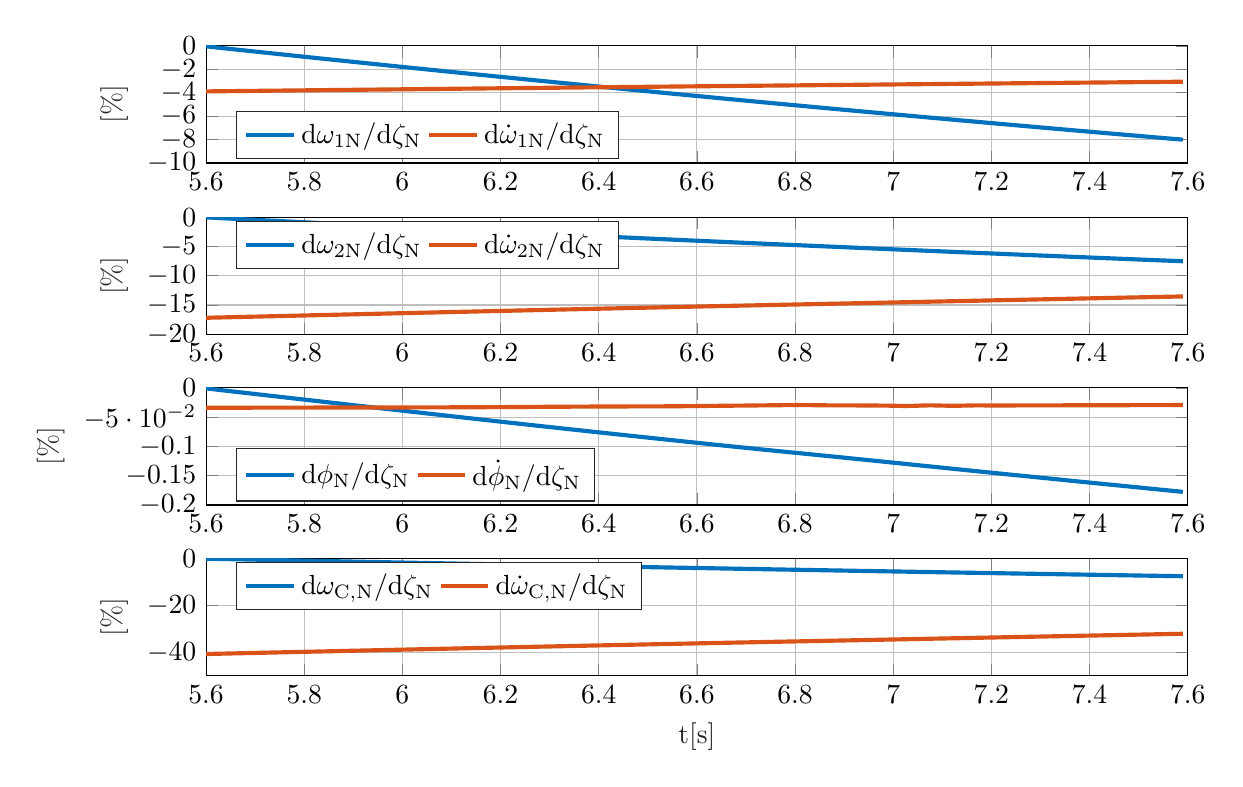
\begin{tikzpicture}

\begin{axis}[%
width=0.959\zwidth,
height=0.186\zheight,
at={(0\zwidth,0.814\zheight)},
scale only axis,
xmin=5.6,
xmax=7.6,
ymin=-10,
ymax=0,
ylabel style={font=\color{white!15!black}},
ylabel={[$\%$]},
axis background/.style={fill=white},
xmajorgrids,
ymajorgrids,
legend style={at={(0.03,0.03)}, anchor=south west, legend columns=2, legend cell align=left, align=left, draw=white!15!black}
]
\addplot [color=mycolor1, line width=1.5pt]
  table[row sep=crcr]{%
5.59	0\\
5.6	-0.044945703992688\\
5.61	-0.0898397666666252\\
5.62	-0.134682095466796\\
5.63	-0.179472823188029\\
5.64	-0.224211857376064\\
5.65	-0.268899330750271\\
5.66	-0.313535150956986\\
5.67	-0.358119450639846\\
5.68	-0.402652137545643\\
5.69	-0.447133344242007\\
5.7	-0.491562978576001\\
5.71	-0.535940714904561\\
5.72	-0.58026736756555\\
5.73	-0.624542631001466\\
5.74	-0.668766403245242\\
5.75	-0.712938816305\\
5.76	-0.757059778299043\\
5.77	-0.801129421506355\\
5.78	-0.845147654212304\\
5.79	-0.889114608639083\\
5.8	-0.933030193156346\\
5.81	-0.97689453987462\\
5.82	-1.0207075572291\\
5.83	-1.06446937723152\\
5.84	-1.10817990841199\\
5.85	-1.15183928271298\\
5.86	-1.19544740877786\\
5.87	-1.23900441848349\\
5.88	-1.28251022057883\\
5.89	-1.3259649468623\\
5.9	-1.36936850617716\\
5.91	-1.41272103023711\\
5.92	-1.45602625212659\\
5.93	-1.49928428028689\\
5.94	-1.542489310731\\
5.95	-1.5856453894372\\
5.96	-1.62875075529345\\
5.97	-1.67180513745478\\
5.98	-1.71480855750988\\
5.99	-1.7577585872647\\
6	-1.80065968057166\\
6.01	-1.84351031580852\\
6.02	-1.88631001395705\\
6.03	-1.92905886855802\\
6.04	-1.97175655586622\\
6.05	-2.01440342096949\\
6.06	-2.05699987805818\\
6.07	-2.09954559342704\\
6.08	-2.14204060636044\\
6.09	-2.18448496038071\\
6.1	-2.22687869460905\\
6.11	-2.26922184511327\\
6.12	-2.31151444922785\\
6.13	-2.35375655031956\\
6.14	-2.39594820167438\\
6.15	-2.43808946154562\\
6.16	-2.48018039390069\\
6.17	-2.52222106257538\\
6.18	-2.56421153074752\\
6.19	-2.60615185926518\\
6.2	-2.64804210702314\\
6.21	-2.68988233906092\\
6.22	-2.73167262885907\\
6.23	-2.77341305571564\\
6.24	-2.81510370449221\\
6.25	-2.85674466182303\\
6.26	-2.89833517837814\\
6.27	-2.93987701610534\\
6.28	-2.98136942001216\\
6.29	-3.02281247627788\\
6.3	-3.06420627250732\\
6.31	-3.10555089048557\\
6.32	-3.14684640503208\\
6.33	-3.18809288329303\\
6.34	-3.22929038617481\\
6.35	-3.27043897284302\\
6.36	-3.31153870607115\\
6.37	-3.35258965450892\\
6.38	-3.39359189059612\\
6.39	-3.4345454851866\\
6.4	-3.47545050177322\\
6.41	-3.51630699340667\\
6.42	-3.55711500394087\\
6.43	-3.59787457297755\\
6.44	-3.63858574158329\\
6.45	-3.67924855585184\\
6.46	-3.71986306633925\\
6.47	-3.76042932384144\\
6.48	-3.80094737395113\\
6.49	-3.8414172532763\\
6.5	-3.88183887078191\\
6.51	-3.92221221261783\\
6.52	-3.96253763198955\\
6.53	-4.00281508334993\\
6.54	-4.04304451056621\\
6.55	-4.08322583857767\\
6.56	-4.12335954119602\\
6.57	-4.16344554360341\\
6.58	-4.20348396004987\\
6.59	-4.24347490005832\\
6.6	-4.28341847221072\\
6.61	-4.32331479201733\\
6.62	-4.36316398822495\\
6.63	-4.40296620416692\\
6.64	-4.44272158519556\\
6.65	-4.48243027319373\\
6.66	-4.52209240127417\\
6.67	-4.56170808888968\\
6.68	-4.60127744911321\\
6.69	-4.6408005959343\\
6.7	-4.6802776503752\\
6.71	-4.71970874446486\\
6.72	-4.75909401944586\\
6.73	-4.79843361975218\\
6.74	-4.83772768680566\\
6.75	-4.87697635527695\\
6.76	-4.9161793219178\\
6.77	-4.9553375759735\\
6.78	-4.99445080687109\\
6.79	-5.03351835329343\\
6.8	-5.07254012659709\\
6.81	-5.11151874223388\\
6.82	-5.15045274720747\\
6.83	-5.18934189760276\\
6.84	-5.22818604439243\\
6.85	-5.26698501496273\\
6.86	-5.30573865575264\\
6.87	-5.34444686310295\\
6.88	-5.38310959053224\\
6.89	-5.42172683113298\\
6.9	-5.46029858529996\\
6.91	-5.4988248298501\\
6.92	-5.53730550185265\\
6.93	-5.57574050243072\\
6.94	-5.61412971523618\\
6.95	-5.65247303022761\\
6.96	-5.6907703598913\\
6.97	-5.72902155419135\\
6.98	-5.76722655061125\\
6.99	-5.80538534125524\\
7	-5.84349795996407\\
7.01	-5.8815633183078\\
7.02	-5.91958140352306\\
7.03	-5.95755338035772\\
7.04	-5.99547842319015\\
7.05	-6.03335632164029\\
7.06	-6.07118861981488\\
7.07	-6.10897425602658\\
7.08	-6.14671517992658\\
7.09	-6.18440986386628\\
7.1	-6.22205913310407\\
7.11	-6.25966210798164\\
7.12	-6.29721771549616\\
7.13	-6.3347275620655\\
7.14	-6.37219096750693\\
7.15	-6.40960666004679\\
7.16	-6.44697655911584\\
7.17	-6.4843020816546\\
7.18	-6.52158159972655\\
7.19	-6.55881608444028\\
7.2	-6.59600476941682\\
7.21	-6.63314747276347\\
7.22	-6.67024289527726\\
7.23	-6.70729352337727\\
7.24	-6.7442982478827\\
7.25	-6.78125699303573\\
7.26	-6.8181686811093\\
7.27	-6.85503393663357\\
7.28	-6.89185569454378\\
7.29	-6.92863251485293\\
7.3	-6.96536374826917\\
7.31	-7.0020493553266\\
7.32	-7.03868704194831\\
7.33	-7.07528138018902\\
7.34	-7.11183027938533\\
7.35	-7.14833234278885\\
7.36	-7.18478672838925\\
7.37	-7.22119676057664\\
7.38	-7.25756415078415\\
7.39	-7.29388633758086\\
7.4	-7.33016323542594\\
7.41	-7.36639484313196\\
7.42	-7.40257835146193\\
7.43	-7.43871936585839\\
7.44	-7.47481529399544\\
7.45	-7.51086608934067\\
7.46	-7.54686835396161\\
7.47	-7.5828263595473\\
7.48	-7.61874141854861\\
7.49	-7.65460911080445\\
7.5	-7.69042864006661\\
7.51	-7.72620916039267\\
7.52	-7.76193638208817\\
7.53	-7.79762242644786\\
7.54	-7.83326358826925\\
7.55	-7.86886151722416\\
7.56	-7.90441756584187\\
7.57	-7.93992662227347\\
7.58	-7.97539327384807\\
7.59	-8.01081523293402\\
};
\addlegendentry{d$\omega_{1\mathrm{N}}/$d$\zeta_\mathrm{N}$}

\addplot [color=mycolor2, line width=1.5pt]
  table[row sep=crcr]{%
5.59	-3.89399544161951\\
5.6	-3.88951871391663\\
5.61	-3.88504372964221\\
5.62	-3.88057048869124\\
5.63	-3.87609899223312\\
5.64	-3.87162924023712\\
5.65	-3.86716123378129\\
5.66	-3.86269497290835\\
5.67	-3.85823045860431\\
5.68	-3.85376769098497\\
5.69	-3.84930667094448\\
5.7	-3.84484739867144\\
5.71	-3.84038991421432\\
5.72	-3.83593415443879\\
5.73	-3.83148013499527\\
5.74	-3.82702785715959\\
5.75	-3.82257732508624\\
5.76	-3.81812854336069\\
5.77	-3.81368151558184\\
5.78	-3.8092362433754\\
5.79	-3.8047927265687\\
5.8	-3.80035096415407\\
5.81	-3.79591095484434\\
5.82	-3.79147269820764\\
5.83	-3.78703619423597\\
5.84	-3.78260144399872\\
5.85	-3.77816844833411\\
5.86	-3.77373720862933\\
5.87	-3.76930772530918\\
5.88	-3.76487999925072\\
5.89	-3.76045403024386\\
5.9	-3.75602981892802\\
5.91	-3.75160736497095\\
5.92	-3.74718651635695\\
5.93	-3.7427671269498\\
5.94	-3.7383493348955\\
5.95	-3.73393308420237\\
5.96	-3.72951850298115\\
5.97	-3.72510569538542\\
5.98	-3.72069473810614\\
5.99	-3.71628577602629\\
6	-3.71187864092863\\
6.01	-3.70747326589323\\
6.02	-3.70306929139734\\
6.03	-3.6986665016989\\
6.04	-3.6942654149309\\
6.05	-3.68986682976082\\
6.06	-3.68547158174196\\
6.07	-3.6810801984706\\
6.08	-3.67669272227378\\
6.09	-3.67230882690183\\
6.1	-3.66792813968142\\
6.11	-3.66355055635924\\
6.12	-3.65917640720749\\
6.13	-3.65480636904884\\
6.14	-3.65044120851056\\
6.15	-3.64608144860669\\
6.16	-3.64172728383532\\
6.17	-3.63737860400877\\
6.18	-3.63303519500655\\
6.19	-3.62869700065023\\
6.2	-3.62436424261205\\
6.21	-3.62003740905875\\
6.22	-3.61571715129238\\
6.23	-3.61140403669745\\
6.24	-3.60709838091456\\
6.25	-3.60280023530564\\
6.26	-3.59850966008729\\
6.27	-3.59422638456782\\
6.28	-3.58995059807891\\
6.29	-3.58568233801727\\
6.3	-3.58142142779831\\
6.31	-3.5771673706987\\
6.32	-3.57291944671346\\
6.33	-3.56867697357259\\
6.34	-3.56443959996456\\
6.35	-3.56020744910621\\
6.36	-3.55598099247911\\
6.37	-3.55176070694948\\
6.38	-3.54754671541499\\
6.39	-3.54333860822921\\
6.4	-3.53913555357969\\
6.41	-3.53493663873638\\
6.42	-3.53074124812871\\
6.43	-3.52654927663167\\
6.44	-3.5223610604668\\
6.45	-3.51817707157259\\
6.46	-3.51399755051498\\
6.47	-3.50982227450239\\
6.48	-3.5056505825738\\
6.49	-3.50148163200256\\
6.5	-3.49731473716363\\
6.51	-3.49314963559173\\
6.52	-3.48898680043683\\
6.53	-3.4848278088606\\
6.54	-3.48067494591362\\
6.55	-3.47653054521707\\
6.56	-3.47239592589058\\
6.57	-3.46827141295441\\
6.58	-3.46415659778379\\
6.59	-3.46005111219038\\
6.6	-3.45595521324574\\
6.61	-3.45186983758748\\
6.62	-3.44779620301549\\
6.63	-3.44373518961121\\
6.64	-3.43968685814627\\
6.65	-3.43565052635926\\
6.66	-3.43162511015514\\
6.67	-3.42760968800189\\
6.68	-3.4236039222113\\
6.69	-3.41960821149057\\
6.7	-3.41562344975532\\
6.71	-3.41165058406614\\
6.72	-3.4076901774599\\
6.73	-3.40374222548321\\
6.74	-3.39980625146493\\
6.75	-3.39588160924228\\
6.76	-3.39196792000385\\
6.77	-3.38806484312652\\
6.78	-3.38417239425555\\
6.79	-3.38028984930336\\
6.8	-3.37641428505386\\
6.81	-3.37254043605126\\
6.82	-3.36866213229465\\
6.83	-3.36477314998213\\
6.84	-3.36086964671643\\
6.85	-3.35695144576054\\
6.86	-3.35302181070907\\
6.87	-3.34908576620075\\
6.88	-3.34514781294463\\
6.89	-3.34121007990021\\
6.9	-3.33727172913527\\
6.91	-3.33332973980706\\
6.92	-3.32938055453741\\
6.93	-3.32542171742545\\
6.94	-3.32145277249434\\
6.95	-3.31747511918754\\
6.96	-3.31349107041627\\
6.97	-3.30950263591963\\
6.98	-3.30550944862576\\
6.99	-3.30150468054594\\
7	-3.29747849223202\\
7.01	-3.29342586859521\\
7.02	-3.2893543742003\\
7.03	-3.28528218466438\\
7.04	-3.28123052677097\\
7.05	-3.27721573115068\\
7.06	-3.27323865233668\\
7.07	-3.26928737389703\\
7.08	-3.26533959362946\\
7.09	-3.26137429367575\\
7.1	-3.25738039199565\\
7.11	-3.25335933032673\\
7.12	-3.24932472258048\\
7.13	-3.24529550471252\\
7.14	-3.2412864817229\\
7.15	-3.2373057224405\\
7.16	-3.23334777855357\\
7.17	-3.22940084062943\\
7.18	-3.2254520299094\\
7.19	-3.22149174855007\\
7.2	-3.21751694224798\\
7.21	-3.21353158997193\\
7.22	-3.20954452611413\\
7.23	-3.20556458117573\\
7.24	-3.20159732528572\\
7.25	-3.19764399313894\\
7.26	-3.19370105979065\\
7.27	-3.18976207678246\\
7.28	-3.18582175366972\\
7.29	-3.18187727464645\\
7.3	-3.1779284990403\\
7.31	-3.17397786457705\\
7.32	-3.17002963099509\\
7.33	-3.16608662060757\\
7.34	-3.16215051232041\\
7.35	-3.15822115198778\\
7.36	-3.15429661463531\\
7.37	-3.15037433660891\\
7.38	-3.14645272308415\\
7.39	-3.1425310815737\\
7.4	-3.13860966410256\\
7.41	-3.13468958204747\\
7.42	-3.13077246797895\\
7.43	-3.12685891065621\\
7.44	-3.12294942112966\\
7.45	-3.11904374443314\\
7.46	-3.11514138639393\\
7.47	-3.1112413429251\\
7.48	-3.10734306155713\\
7.49	-3.1034465611503\\
7.5	-3.09955217374046\\
7.51	-3.09565980106647\\
7.52	-3.09177063035473\\
7.53	-3.08788415879222\\
7.54	-3.08400064185992\\
7.55	-3.08011984644078\\
7.56	-3.07624147821042\\
7.57	-3.07236562897651\\
7.58	-3.06849195172669\\
7.59	-3.06462054890528\\
};
\addlegendentry{d$\dot{\omega}_{1\mathrm{N}}/$d$\zeta_\mathrm{N}$}

\end{axis}

\begin{axis}[%
width=0.959\zwidth,
height=0.186\zheight,
at={(0\zwidth,0.542\zheight)},
scale only axis,
xmin=5.6,
xmax=7.6,
ymin=-20,
ymax=0,
ylabel style={font=\color{white!15!black}},
ylabel={[$\%$]},
axis background/.style={fill=white},
xmajorgrids,
ymajorgrids,
legend style={at={(0.03,0.97)}, anchor=north west, legend columns=2, legend cell align=left, align=left, draw=white!15!black}
]
\addplot [color=mycolor1, line width=1.5pt]
  table[row sep=crcr]{%
5.59	0\\
5.6	-0.0422456541872118\\
5.61	-0.0844427693350979\\
5.62	-0.126591258448752\\
5.63	-0.168691246345544\\
5.64	-0.210742646125268\\
5.65	-0.252745582534368\\
5.66	-0.294699968767194\\
5.67	-0.336605929499008\\
5.68	-0.378463378018576\\
5.69	-0.420272438929723\\
5.7	-0.462033025615463\\
5.71	-0.503744831995268\\
5.72	-0.545408623486829\\
5.73	-0.587024112888574\\
5.74	-0.628591204358952\\
5.75	-0.670110021975891\\
5.76	-0.711580479377355\\
5.77	-0.753002700895856\\
5.78	-0.794376600326384\\
5.79	-0.835702301948078\\
5.8	-0.876979719635152\\
5.81	-0.918208977561775\\
5.82	-0.95938998966377\\
5.83	-1.00052288002247\\
5.84	-1.04160756266288\\
5.85	-1.08264416160124\\
5.86	-1.12363259096901\\
5.87	-1.16457297472076\\
5.88	-1.20546522708722\\
5.89	-1.2463094719492\\
5.9	-1.28710562362608\\
5.91	-1.32785380591904\\
5.92	-1.36855752765274\\
5.93	-1.40921689075399\\
5.94	-1.44982643990215\\
5.95	-1.49038997801904\\
5.96	-1.53090584978894\\
5.97	-1.57137380063753\\
5.98	-1.61179385085657\\
5.99	-1.65216371812235\\
6	-1.6924875887284\\
6.01	-1.73276403246178\\
6.02	-1.7729925990806\\
6.03	-1.8131733765063\\
6.04	-1.85330606044221\\
6.05	-1.89339097524551\\
6.06	-1.93342851022464\\
6.07	-1.97341835172121\\
6.08	-2.01336053665967\\
6.09	-2.05325510594778\\
6.1	-2.09310209635661\\
6.11	-2.13290154178723\\
6.12	-2.17265347733131\\
6.13	-2.21235794375043\\
6.14	-2.25201499112947\\
6.15	-2.29162467422228\\
6.16	-2.3311870531535\\
6.17	-2.37070218792409\\
6.18	-2.41017013791653\\
6.19	-2.44959096032356\\
6.2	-2.48896471050192\\
6.21	-2.52829144958399\\
6.22	-2.56757124663607\\
6.23	-2.60680417619248\\
6.24	-2.64599031801688\\
6.25	-2.68512975353909\\
6.26	-2.72422177844407\\
6.27	-2.76326804883311\\
6.28	-2.80226785506883\\
6.29	-2.84122127815343\\
6.3	-2.88012840042898\\
6.31	-2.91898929876746\\
6.32	-2.95780404349364\\
6.33	-2.99657269771999\\
6.34	-3.03529531869401\\
6.35	-3.07397196202705\\
6.36	-3.11260268672154\\
6.37	-3.15118755730319\\
6.38	-3.18972664186005\\
6.39	-3.22822000698953\\
6.4	-3.26666771237026\\
6.41	-3.30506980786596\\
6.42	-3.34342633469611\\
6.43	-3.38173733008341\\
6.44	-3.42000283262742\\
6.45	-3.45822288565289\\
6.46	-3.49639753667878\\
6.47	-3.53452683344951\\
6.48	-3.57261081881888\\
6.49	-3.6106495271957\\
6.5	-3.64864287301373\\
6.51	-3.68659084325488\\
6.52	-3.7244937699063\\
6.53	-3.76235161015705\\
6.54	-3.80016431124645\\
6.55	-3.83793180262295\\
6.56	-3.87565452963469\\
6.57	-3.9133324219584\\
6.58	-3.95096558698071\\
6.59	-3.98855412764507\\
6.6	-4.02609814601057\\
6.61	-4.06359775064834\\
6.62	-4.10105306257089\\
6.63	-4.13846421650103\\
6.64	-4.17583134905922\\
6.65	-4.21315459360493\\
6.66	-4.25043407525433\\
6.67	-4.28766990628426\\
6.68	-4.32486219297497\\
6.69	-4.36201104246824\\
6.7	-4.39911656851609\\
6.71	-4.436178895216\\
6.72	-4.47319815532561\\
6.73	-4.51017448460223\\
6.74	-4.547108015972\\
6.75	-4.58399887601539\\
6.76	-4.62084677970138\\
6.77	-4.65765265684774\\
6.78	-4.69441621553874\\
6.79	-4.73113683418496\\
6.8	-4.76781442946806\\
6.81	-4.80445145972028\\
6.82	-4.84104655923202\\
6.83	-4.87759949874099\\
6.84	-4.91411013817252\\
6.85	-4.95057831528236\\
6.86	-4.98700388573447\\
6.87	-5.02338675209682\\
6.88	-5.05972687068029\\
6.89	-5.09602423499231\\
6.9	-5.13227884540396\\
6.91	-5.16849068012483\\
6.92	-5.20465968000467\\
6.93	-5.24078575210648\\
6.94	-5.27686878707155\\
6.95	-5.31290868146908\\
6.96	-5.3489053530426\\
6.97	-5.38485866076941\\
6.98	-5.42076854588859\\
6.99	-5.45663500097872\\
7	-5.4924580578476\\
7.01	-5.52823669345118\\
7.02	-5.56397089579284\\
7.03	-5.59966175964987\\
7.04	-5.63530850899869\\
7.05	-5.67091094609753\\
7.06	-5.70647052229308\\
7.07	-5.74198623967739\\
7.08	-5.77745993077909\\
7.09	-5.81289015972091\\
7.1	-5.84827770218502\\
7.11	-5.88362173135733\\
7.12	-5.91892123869416\\
7.13	-5.95417773411007\\
7.14	-5.98939057828336\\
7.15	-6.02455857584039\\
7.16	-6.05968353090481\\
7.17	-6.09476677529643\\
7.18	-6.12980677887473\\
7.19	-6.16480445441033\\
7.2	-6.19975908156337\\
7.21	-6.23467048936812\\
7.22	-6.26953745666939\\
7.23	-6.30436232051814\\
7.24	-6.33914403836604\\
7.25	-6.37388253900632\\
7.26	-6.40857680945484\\
7.27	-6.44322743672402\\
7.28	-6.47783717943698\\
7.29	-6.5124046841119\\
7.3	-6.54692934046224\\
7.31	-6.58141111139296\\
7.32	-6.61584784064058\\
7.33	-6.65024382560009\\
7.34	-6.68459710120171\\
7.35	-6.71890635460478\\
7.36	-6.75317079438154\\
7.37	-6.78739354521404\\
7.38	-6.8215762157235\\
7.39	-6.85571639835333\\
7.4	-6.88981401270146\\
7.41	-6.92386905765178\\
7.42	-6.95787889272825\\
7.43	-6.99184878663438\\
7.44	-7.02577630277457\\
7.45	-7.05966139741178\\
7.46	-7.09350087673953\\
7.47	-7.1272987558312\\
7.48	-7.16105626829399\\
7.49	-7.19476925950177\\
7.5	-7.22843698103984\\
7.51	-7.26206803704863\\
7.52	-7.29564899626696\\
7.53	-7.32919125181989\\
7.54	-7.36269132108973\\
7.55	-7.3961507546466\\
7.56	-7.42957082376848\\
7.57	-7.46294672369358\\
7.58	-7.49628276617369\\
7.59	-7.5295768010034\\
};
\addlegendentry{d$\omega_{2\mathrm{N}}/$d$\zeta_\mathrm{N}$}

\addplot [color=mycolor2, line width=1.5pt]
  table[row sep=crcr]{%
5.59	-17.1979972163496\\
5.6	-17.1782255572076\\
5.61	-17.1584615979917\\
5.62	-17.1387053382383\\
5.63	-17.1189567831121\\
5.64	-17.0992159324778\\
5.65	-17.0794827910958\\
5.66	-17.0597573591553\\
5.67	-17.0400396410107\\
5.68	-17.0203296371742\\
5.69	-17.0006273515942\\
5.7	-16.9809327851034\\
5.71	-16.9612461145783\\
5.72	-16.9415670611832\\
5.73	-16.9218956940386\\
5.74	-16.9022320187797\\
5.75	-16.8825760537544\\
5.76	-16.8629278192151\\
5.77	-16.8432873310561\\
5.78	-16.8236545964579\\
5.79	-16.8040296146574\\
5.8	-16.7844123812047\\
5.81	-16.7648028904144\\
5.82	-16.7452011403797\\
5.83	-16.7256071310649\\
5.84	-16.7060208671931\\
5.85	-16.6864423524661\\
5.86	-16.6668715930108\\
5.87	-16.6473085907034\\
5.88	-16.6277533494171\\
5.89	-16.6082058682244\\
5.9	-16.5886661499493\\
5.91	-16.569134193124\\
5.92	-16.5496093263649\\
5.93	-16.5300909042557\\
5.94	-16.5105795369232\\
5.95	-16.4910749770781\\
5.96	-16.4715777905273\\
5.97	-16.4520884372688\\
5.98	-16.4326072560123\\
5.99	-16.4131348866392\\
6	-16.393670586211\\
6.01	-16.3742140591732\\
6.02	-16.3547637176777\\
6.03	-16.3353186088907\\
6.04	-16.3158810211689\\
6.05	-16.2964544818611\\
6.06	-16.2770426812242\\
6.07	-16.2576479494101\\
6.08	-16.2382704733572\\
6.09	-16.2189088121704\\
6.1	-16.199561319922\\
6.11	-16.1802275361723\\
6.12	-16.1609089195835\\
6.13	-16.1416084593713\\
6.14	-16.1223295413776\\
6.15	-16.1030744755167\\
6.16	-16.0838441207973\\
6.17	-16.0646379905714\\
6.18	-16.045455139166\\
6.19	-16.0262953184671\\
6.2	-16.0071595074992\\
6.21	-15.9880498622723\\
6.22	-15.968969259289\\
6.23	-15.9499202044277\\
6.24	-15.9309040917281\\
6.25	-15.9119211480332\\
6.26	-15.8929716392911\\
6.27	-15.8740543699815\\
6.28	-15.8551701762946\\
6.29	-15.8363192233959\\
6.3	-15.8175007313912\\
6.31	-15.7987125064809\\
6.32	-15.7799513687319\\
6.33	-15.7612143048703\\
6.34	-15.7424997633129\\
6.35	-15.7238082882527\\
6.36	-15.7051419620085\\
6.37	-15.6865028906794\\
6.38	-15.6678916170488\\
6.39	-15.6493063318958\\
6.4	-15.630743361485\\
6.41	-15.6121986747055\\
6.42	-15.5936695528625\\
6.43	-15.5751555316683\\
6.44	-15.5566580960588\\
6.45	-15.5381793303709\\
6.46	-15.519720297074\\
6.47	-15.5012800121999\\
6.48	-15.4828555565859\\
6.49	-15.4644432082935\\
6.5	-15.4460399392311\\
6.51	-15.4276445902087\\
6.52	-15.409259250914\\
6.53	-15.390890886949\\
6.54	-15.3725495903365\\
6.55	-15.3542456676149\\
6.56	-15.3359849447313\\
6.57	-15.3177688571528\\
6.58	-15.2995956001703\\
6.59	-15.2814635476636\\
6.6	-15.2633738350011\\
6.61	-15.2453305988827\\
6.62	-15.2273392177726\\
6.63	-15.2094035785894\\
6.64	-15.1915239497328\\
6.65	-15.1736973179667\\
6.66	-15.1559188953385\\
6.67	-15.138184611863\\
6.68	-15.1204929761257\\
6.69	-15.1028457490339\\
6.7	-15.0852468786045\\
6.71	-15.0677005475702\\
6.72	-15.0502092426083\\
6.73	-15.0327729440499\\
6.74	-15.0153895466564\\
6.75	-14.9980561966228\\
6.76	-14.9807712209112\\
6.77	-14.9635331151461\\
6.78	-14.9463419484251\\
6.79	-14.9291945227845\\
6.8	-14.9120779277154\\
6.81	-14.8949689081078\\
6.82	-14.8778402138883\\
6.83	-14.8606643573711\\
6.84	-14.8434243684431\\
6.85	-14.8261194665391\\
6.86	-14.8087640654637\\
6.87	-14.7913803567478\\
6.88	-14.7739882179658\\
6.89	-14.7565970517586\\
6.9	-14.7392031573619\\
6.91	-14.7217931930948\\
6.92	-14.7043514476457\\
6.93	-14.6868670744221\\
6.94	-14.6693380595834\\
6.95	-14.6517705838321\\
6.96	-14.6341748622382\\
6.97	-14.6165597709005\\
6.98	-14.5989236886316\\
6.99	-14.5812364593267\\
7	-14.5634546266428\\
7.01	-14.5455560412258\\
7.02	-14.5275741122995\\
7.03	-14.5095891132536\\
7.04	-14.4916947930834\\
7.05	-14.4739632767176\\
7.06	-14.456398338238\\
7.07	-14.4389473482137\\
7.08	-14.4215118080159\\
7.09	-14.4039988913759\\
7.1	-14.3863596539891\\
7.11	-14.3686004633519\\
7.12	-14.3507814458852\\
7.13	-14.3329862330462\\
7.14	-14.3152802117506\\
7.15	-14.2976990183244\\
7.16	-14.2802185900676\\
7.17	-14.2627867701157\\
7.18	-14.2453466788804\\
7.19	-14.2278559270771\\
7.2	-14.2103010252432\\
7.21	-14.1926995466646\\
7.22	-14.1750905088127\\
7.23	-14.157512911972\\
7.24	-14.1399913568558\\
7.25	-14.1225312965461\\
7.26	-14.1051171629747\\
7.27	-14.0877204762486\\
7.28	-14.0703178708937\\
7.29	-14.0528969107823\\
7.3	-14.035456974629\\
7.31	-14.0180088287541\\
7.32	-14.0005712864742\\
7.33	-13.9831568126551\\
7.34	-13.9657728222576\\
7.35	-13.9484186344894\\
7.36	-13.9310857476187\\
7.37	-13.9137628391587\\
7.38	-13.8964428654987\\
7.39	-13.8791227682382\\
7.4	-13.8618036604568\\
7.41	-13.8444904505975\\
7.42	-13.8271903489781\\
7.43	-13.8099059558782\\
7.44	-13.7926395283738\\
7.45	-13.7753899403961\\
7.46	-13.7581550094103\\
7.47	-13.7409303008235\\
7.48	-13.7237133746299\\
7.49	-13.7065043141282\\
7.5	-13.6893045857674\\
7.51	-13.6721137555734\\
7.52	-13.6549370669825\\
7.53	-13.6377722992996\\
7.54	-13.6206205808673\\
7.55	-13.6034808821142\\
7.56	-13.5863519031439\\
7.57	-13.5692340494294\\
7.58	-13.5521257883749\\
7.59	-13.5350275724307\\
};
\addlegendentry{d$\dot{\omega}_{2\mathrm{N}}/$d$\zeta_\mathrm{N}$}

\end{axis}

\begin{axis}[%
width=0.959\zwidth,
height=0.186\zheight,
at={(0\zwidth,0.271\zheight)},
scale only axis,
xmin=5.6,
xmax=7.6,
ymin=-0.2,
ymax=0,
ylabel style={font=\color{white!15!black}},
ylabel={[$\%$]},
axis background/.style={fill=white},
xmajorgrids,
ymajorgrids,
legend style={at={(0.03,0.03)}, anchor=south west, legend columns=2, legend cell align=left, align=left, draw=white!15!black}
]
\addplot [color=mycolor1, line width=1.5pt]
  table[row sep=crcr]{%
5.59	0\\
5.6	-0.000957952589146475\\
5.61	-0.00191553249632893\\
5.62	-0.00287273923978163\\
5.63	-0.00382957306774724\\
5.64	-0.00478603349225715\\
5.65	-0.00574212077146936\\
5.66	-0.0066978344113001\\
5.67	-0.00765317467992044\\
5.68	-0.00860814107722151\\
5.69	-0.00956273388143146\\
5.7	-0.010516952586464\\
5.71	-0.0114707909882442\\
5.72	-0.0124242580123189\\
5.73	-0.0133773524616121\\
5.74	-0.0143300741179179\\
5.75	-0.0152824228641323\\
5.76	-0.0162343973899681\\
5.77	-0.0171859972704531\\
5.78	-0.0181372215466382\\
5.79	-0.0190880704943656\\
5.8	-0.0200385437995752\\
5.81	-0.0209886421285054\\
5.82	-0.021938365213296\\
5.83	-0.0228877135361074\\
5.84	-0.0238366865376335\\
5.85	-0.0247852844675773\\
5.86	-0.0257335066405109\\
5.87	-0.0266813533248438\\
5.88	-0.027628823921749\\
5.89	-0.0285759188251575\\
5.9	-0.0295226375173297\\
5.91	-0.0304689804366609\\
5.92	-0.0314149767089712\\
5.93	-0.0323606456369449\\
5.94	-0.0333059692113346\\
5.95	-0.0342509684619925\\
5.96	-0.03519561865951\\
5.97	-0.0361398995591609\\
5.98	-0.0370837923961694\\
5.99	-0.0380272643708884\\
6	-0.0389703440552431\\
6.01	-0.039913033784988\\
6.02	-0.0408553821734453\\
6.03	-0.0417974635420599\\
6.04	-0.0427392311550553\\
6.05	-0.0436805487596198\\
6.06	-0.0446212401407108\\
6.07	-0.045561157381712\\
6.08	-0.046500242801751\\
6.09	-0.0474385295034186\\
6.1	-0.0483760927562017\\
6.11	-0.0493129832725475\\
6.12	-0.0502491746658525\\
6.13	-0.0511845571725568\\
6.14	-0.0521189738783986\\
6.15	-0.0530522915888308\\
6.16	-0.053984432505102\\
6.17	-0.0549153889790861\\
6.18	-0.0558451969317502\\
6.19	-0.0567738842541721\\
6.2	-0.0577014325376819\\
6.21	-0.0586277665840077\\
6.22	-0.0595527610842147\\
6.23	-0.0604762861168737\\
6.24	-0.0613982480610953\\
6.25	-0.0623186094665619\\
6.26	-0.0632373459921992\\
6.27	-0.0641545193760003\\
6.28	-0.0650700969811188\\
6.29	-0.0659840673724043\\
6.3	-0.0668964450865939\\
6.31	-0.0678073031796502\\
6.32	-0.068716773076104\\
6.33	-0.0696250064100352\\
6.34	-0.070532113551898\\
6.35	-0.0714381170759222\\
6.36	-0.0723429507663316\\
6.37	-0.0732465119806187\\
6.38	-0.0741487369331966\\
6.39	-0.0750496584508037\\
6.4	-0.0759494119370125\\
6.41	-0.0768481853686393\\
6.42	-0.0777461420542007\\
6.43	-0.078643357016993\\
6.44	-0.079539802992338\\
6.45	-0.0804353920355902\\
6.46	-0.0813300478590661\\
6.47	-0.082223770388665\\
6.48	-0.0831166564982123\\
6.49	-0.0840088686035655\\
6.5	-0.0849005702717969\\
6.51	-0.0857918625567704\\
6.52	-0.0866827248961835\\
6.53	-0.0875729316952796\\
6.54	-0.0884620704614095\\
6.55	-0.0893496347895143\\
6.56	-0.0902352504545\\
6.57	-0.0911187355579587\\
6.58	-0.0920001072218079\\
6.59	-0.0928794501254086\\
6.6	-0.0937567720274247\\
6.61	-0.0946319419721831\\
6.62	-0.0955047250209663\\
6.63	-0.0963748955395795\\
6.64	-0.0972423600851243\\
6.65	-0.0981071856256921\\
6.66	-0.0989695637047271\\
6.67	-0.0998297082501058\\
6.68	-0.100687753955073\\
6.69	-0.101543691085463\\
6.7	-0.102397378522261\\
6.71	-0.103248617802256\\
6.72	-0.104097248974709\\
6.73	-0.104943214608089\\
6.74	-0.105786568665588\\
6.75	-0.106627432051592\\
6.76	-0.107465903518945\\
6.77	-0.108302089522432\\
6.78	-0.109135987754482\\
6.79	-0.109967662390535\\
6.8	-0.110797530014753\\
6.81	-0.111626510363672\\
6.82	-0.112455763300691\\
6.83	-0.113286654910573\\
6.84	-0.114120258576935\\
6.85	-0.114956993098875\\
6.86	-0.115796513357445\\
6.87	-0.116637923763078\\
6.88	-0.117480204503624\\
6.89	-0.118322654723311\\
6.9	-0.119165148772568\\
6.91	-0.120008109928239\\
6.92	-0.120852245454105\\
6.93	-0.121698194530442\\
6.94	-0.122546260931373\\
6.95	-0.123396335161634\\
6.96	-0.124248014596811\\
6.97	-0.125100837989218\\
6.98	-0.12595460194702\\
6.99	-0.126810109325363\\
7	-0.127669200303799\\
7.01	-0.128533522346128\\
7.02	-0.129402683907461\\
7.03	-0.130273849454831\\
7.04	-0.131142869317114\\
7.05	-0.132005602684257\\
7.06	-0.132860433702798\\
7.07	-0.133708380064825\\
7.08	-0.134553371452053\\
7.09	-0.135399914850957\\
7.1	-0.136251411157125\\
7.11	-0.137108895020411\\
7.12	-0.137970720917572\\
7.13	-0.138833271826255\\
7.14	-0.139693120322709\\
7.15	-0.140547607043807\\
7.16	-0.141396759531877\\
7.17	-0.142242394472814\\
7.18	-0.14308703485633\\
7.19	-0.143933128708538\\
7.2	-0.144782014019789\\
7.21	-0.145633574441828\\
7.22	-0.14648642342097\\
7.23	-0.14733863796407\\
7.24	-0.148188746298259\\
7.25	-0.149035977147238\\
7.26	-0.149880591693587\\
7.27	-0.150723740589857\\
7.28	-0.151566642083113\\
7.29	-0.152410109356152\\
7.3	-0.153254484863414\\
7.31	-0.154099528322664\\
7.32	-0.154944471041022\\
7.33	-0.155788610909077\\
7.34	-0.156631440379755\\
7.35	-0.15747278688524\\
7.36	-0.158312904802624\\
7.37	-0.159152316880088\\
7.38	-0.159991413708874\\
7.39	-0.16083042743509\\
7.4	-0.161669422290811\\
7.41	-0.162508245579338\\
7.42	-0.163346583763122\\
7.43	-0.164184256889853\\
7.44	-0.16502109810661\\
7.45	-0.165857095450376\\
7.46	-0.166692306893388\\
7.47	-0.16752695317537\\
7.48	-0.168361169197346\\
7.49	-0.169194983289193\\
7.5	-0.17002837323676\\
7.51	-0.170861362643012\\
7.52	-0.171693714271144\\
7.53	-0.172525509141567\\
7.54	-0.173356676163694\\
7.55	-0.17418724890054\\
7.56	-0.175017279388062\\
7.57	-0.175846749124696\\
7.58	-0.176675743369826\\
7.59	-0.177504248519036\\
};
\addlegendentry{d$\phi_\mathrm{N}/$d$\zeta_\mathrm{N}$}

\addplot [color=mycolor2, line width=1.5pt]
  table[row sep=crcr]{%
5.59	-0.0339612950005583\\
5.6	-0.0339480913607774\\
5.61	-0.0339348655316347\\
5.62	-0.0339216532544169\\
5.63	-0.0339084191995244\\
5.64	-0.0338951984212106\\
5.65	-0.0338819562715799\\
5.66	-0.0338687271267344\\
5.67	-0.0338554770231475\\
5.68	-0.0338422396538845\\
5.69	-0.0338289817384556\\
5.7	-0.0338157362904423\\
5.71	-0.0338023357327321\\
5.72	-0.0337891048385492\\
5.73	-0.0337758911157631\\
5.74	-0.0337626906833229\\
5.75	-0.0337494488374615\\
5.76	-0.0337361889182218\\
5.77	-0.0337228864699641\\
5.78	-0.0337095848139932\\
5.79	-0.0336962670165095\\
5.8	-0.0336829706200978\\
5.81	-0.0336696679200314\\
5.82	-0.0336563844524625\\
5.83	-0.0336430861606021\\
5.84	-0.0336297964737589\\
5.85	-0.0336164849794858\\
5.86	-0.033603179227072\\
5.87	-0.0335898537474256\\
5.88	-0.033576537689509\\
5.89	-0.0335632063121217\\
5.9	-0.03354988662141\\
5.91	-0.0335365525793807\\
5.92	-0.0335234449799578\\
5.93	-0.0335114117730565\\
5.94	-0.0334996344987983\\
5.95	-0.0334874715846761\\
5.96	-0.0334747331229895\\
5.97	-0.0334612746332984\\
5.98	-0.0334472632090828\\
5.99	-0.0334328266514565\\
6	-0.0334184907222575\\
6.01	-0.0334051047277039\\
6.02	-0.0333946750339435\\
6.03	-0.0333852051522122\\
6.04	-0.0333721502127761\\
6.05	-0.0333530563761624\\
6.06	-0.0333277431617298\\
6.07	-0.0332986944696653\\
6.08	-0.0332693571431393\\
6.09	-0.0332423324336149\\
6.1	-0.0332179365985645\\
6.11	-0.0331941559054375\\
6.12	-0.0331678520277513\\
6.13	-0.033136541257617\\
6.14	-0.0330997202654851\\
6.15	-0.0330588988570325\\
6.16	-0.0330166421907029\\
6.17	-0.0329751634643739\\
6.18	-0.0329351636485307\\
6.19	-0.0328955176367416\\
6.2	-0.0328541685625642\\
6.21	-0.0328090435979068\\
6.22	-0.0327591480146043\\
6.23	-0.0327050866992614\\
6.24	-0.032648709181197\\
6.25	-0.0325918912231303\\
6.26	-0.0325354450461247\\
6.27	-0.0324790994886642\\
6.28	-0.0324222967230536\\
6.29	-0.0323652801949796\\
6.3	-0.0323096974605618\\
6.31	-0.0322579029712365\\
6.32	-0.0322114998644303\\
6.33	-0.0321700864355967\\
6.34	-0.0321311668194181\\
6.35	-0.0320912721716639\\
6.36	-0.0320479459731196\\
6.37	-0.03200123218416\\
6.38	-0.0319537884853713\\
6.39	-0.0319095004403438\\
6.4	-0.0318713847510866\\
6.41	-0.0318399585819705\\
6.42	-0.0318129811454151\\
6.43	-0.0317867286309232\\
6.44	-0.0317580347341597\\
6.45	-0.0317259762752609\\
6.46	-0.0316923126529197\\
6.47	-0.0316604278771605\\
6.48	-0.0316334788052746\\
6.49	-0.0316127328724354\\
6.5	-0.0315969933741697\\
6.51	-0.031583077458272\\
6.52	-0.0315652671192933\\
6.53	-0.0315356352996463\\
6.54	-0.0314887678247969\\
6.55	-0.0314251709767181\\
6.56	-0.0313513668294501\\
6.57	-0.0312753202847137\\
6.58	-0.0312020146617577\\
6.59	-0.0311310311747927\\
6.6	-0.0310579212129432\\
6.61	-0.0309777630501595\\
6.62	-0.0308887419027217\\
6.63	-0.0307935051119607\\
6.64	-0.0306977548176029\\
6.65	-0.0306070908033711\\
6.66	-0.0305243762541452\\
6.67	-0.0304484222595299\\
6.68	-0.0303748022088223\\
6.69	-0.0302981595028513\\
6.7	-0.0302149407536259\\
6.71	-0.0301248514915629\\
6.72	-0.0300306911886204\\
6.73	-0.0299365984645509\\
6.74	-0.0298459770752643\\
6.75	-0.029760056029132\\
6.76	-0.0296775800346425\\
6.77	-0.0295961686960729\\
6.78	-0.0295157483174204\\
6.79	-0.029442750958011\\
6.8	-0.0293919788922511\\
6.81	-0.0293780893891727\\
6.82	-0.0294124360511792\\
6.83	-0.0294925702392909\\
6.84	-0.0296006763589669\\
6.85	-0.0297097478118101\\
6.86	-0.0297947544274306\\
6.87	-0.0298429793841433\\
6.88	-0.029858457160387\\
6.89	-0.0298585816400245\\
6.9	-0.0298649672954988\\
6.91	-0.0298934225495928\\
6.92	-0.02994776203446\\
6.93	-0.0300199220301325\\
6.94	-0.0300952844013984\\
6.95	-0.0301603874783165\\
6.96	-0.0302086950487004\\
6.97	-0.0302424242270073\\
6.98	-0.030281559451358\\
6.99	-0.0303727398931871\\
7	-0.0305347435828486\\
7.01	-0.0307268453032442\\
7.02	-0.0308620792447624\\
7.03	-0.0308658012184329\\
7.04	-0.0307102481633164\\
7.05	-0.0304412817394103\\
7.06	-0.0301604835537589\\
7.07	-0.0299764329264812\\
7.08	-0.0299487963623133\\
7.09	-0.0300768398705268\\
7.1	-0.0302875534657505\\
7.11	-0.0304857304170493\\
7.12	-0.0305815525124053\\
7.13	-0.0305442411164577\\
7.14	-0.0303922259544392\\
7.15	-0.0301916498980782\\
7.16	-0.0300231872273249\\
7.17	-0.0299371572381942\\
7.18	-0.0299500292326393\\
7.19	-0.0300338294777982\\
7.2	-0.0301400336453216\\
7.21	-0.0302165459241742\\
7.22	-0.0302276748732785\\
7.23	-0.0301758140072778\\
7.24	-0.0300808170600517\\
7.25	-0.0299786317472831\\
7.26	-0.0299042016560773\\
7.27	-0.0298737562706107\\
7.28	-0.0298811716707542\\
7.29	-0.0299115079817666\\
7.3	-0.0299426234207659\\
7.31	-0.0299545811356957\\
7.32	-0.0299372692641833\\
7.33	-0.0298976554692479\\
7.34	-0.0298462560996946\\
7.35	-0.0297976414710705\\
7.36	-0.0297629731539151\\
7.37	-0.0297440749455439\\
7.38	-0.0297374458608148\\
7.39	-0.0297371319855323\\
7.4	-0.0297347580826538\\
7.41	-0.0297242935407058\\
7.42	-0.0297032048900553\\
7.43	-0.0296753193381895\\
7.44	-0.0296447140297945\\
7.45	-0.0296161036739976\\
7.46	-0.0295928732622999\\
7.47	-0.0295746030141124\\
7.48	-0.0295601088646911\\
7.49	-0.0295470965990519\\
7.5	-0.0295321053828777\\
7.51	-0.0295149522831685\\
7.52	-0.0294944490810037\\
7.53	-0.0294724780155146\\
7.54	-0.0294502038896365\\
7.55	-0.029428782911946\\
7.56	-0.0294089900615825\\
7.57	-0.0293907445217317\\
7.58	-0.0293732652485291\\
7.59	-0.0293559629768335\\
};
\addlegendentry{d$\dot{\phi}_\mathrm{N}/$d$\zeta_\mathrm{N}$}

\end{axis}

\begin{axis}[%
width=0.959\zwidth,
height=0.186\zheight,
at={(0\zwidth,0\zheight)},
scale only axis,
xmin=5.6,
xmax=7.6,
xlabel style={font=\color{white!15!black}},
xlabel={t[s]},
ymin=-50,
ymax=0,
ylabel style={font=\color{white!15!black}},
ylabel={[$\%$]},
axis background/.style={fill=white},
xmajorgrids,
ymajorgrids,
legend style={at={(0.03,0.97)}, anchor=north west, legend columns=2, legend cell align=left, align=left, draw=white!15!black}
]
\addplot [color=mycolor1, line width=1.5pt]
  table[row sep=crcr]{%
5.59	0\\
5.6	-0.0422458643071475\\
5.61	-0.0844431894415481\\
5.62	-0.126591888304617\\
5.63	-0.168692085816369\\
5.64	-0.210743694974907\\
5.65	-0.252746840627343\\
5.66	-0.294701435868298\\
5.67	-0.336607605471724\\
5.68	-0.378465262628635\\
5.69	-0.420274532039569\\
5.7	-0.462035326991753\\
5.71	-0.503747341887846\\
5.72	-0.545411341209797\\
5.73	-0.587027038195691\\
5.74	-0.628594337014806\\
5.75	-0.670113361903713\\
5.76	-0.711584026432554\\
5.77	-0.753006455005042\\
5.78	-0.794380561290581\\
5.79	-0.835706469617773\\
5.8	-0.876984093751951\\
5.81	-0.918213557947877\\
5.82	-0.959394776067205\\
5.83	-1.00052787229022\\
5.84	-1.04161276057386\\
5.85	-1.08264956502277\\
5.86	-1.12363819968844\\
5.87	-1.16457878859955\\
5.88	-1.20547124590222\\
5.89	-1.24631569554931\\
5.9	-1.28711205178175\\
5.91	-1.32786043847652\\
5.92	-1.36856436377645\\
5.93	-1.40922392715753\\
5.94	-1.4498336756429\\
5.95	-1.49039741402454\\
5.96	-1.53091348752897\\
5.97	-1.5713816419985\\
5.98	-1.61180189724195\\
5.99	-1.65217197055686\\
6	-1.69249604673391\\
6.01	-1.73277269309917\\
6.02	-1.77300145360892\\
6.03	-1.81318242195639\\
6.04	-1.85331530698204\\
6.05	-1.89340044013793\\
6.06	-1.93343821125583\\
6.07	-1.97342829949559\\
6.08	-2.01337073181764\\
6.09	-2.05326554161022\\
6.1	-2.09311276473028\\
6.11	-2.13291244090036\\
6.12	-2.17266461428455\\
6.13	-2.21236933282454\\
6.14	-2.25202664806043\\
6.15	-2.29163661038174\\
6.16	-2.33119927249797\\
6.17	-2.3707146880124\\
6.18	-2.41018291428138\\
6.19	-2.44960401175035\\
6.2	-2.48897804172229\\
6.21	-2.52830507132196\\
6.22	-2.5675851724915\\
6.23	-2.60681841801695\\
6.24	-2.64600488231564\\
6.25	-2.68514464139526\\
6.26	-2.72423698858994\\
6.27	-2.76328358079156\\
6.28	-2.80228370997245\\
6.29	-2.84123745643137\\
6.3	-2.88014489774797\\
6.31	-2.91900610398826\\
6.32	-2.95782114084295\\
6.33	-2.996590072586\\
6.34	-3.03531296368024\\
6.35	-3.07398987976498\\
6.36	-3.11262088694422\\
6.37	-3.15120604961685\\
6.38	-3.18974542818836\\
6.39	-3.22823907802402\\
6.4	-3.26668705008198\\
6.41	-3.30508939273116\\
6.42	-3.34344615366887\\
6.43	-3.38175738088282\\
6.44	-3.42002312212586\\
6.45	-3.45824342339168\\
6.46	-3.49641832711333\\
6.47	-3.53454787125292\\
6.48	-3.57263208953856\\
6.49	-3.61067101271527\\
6.5	-3.64866455867591\\
6.51	-3.68661272360337\\
6.52	-3.72451585601578\\
6.53	-3.76237393601762\\
6.54	-3.80018692649935\\
6.55	-3.83795475544556\\
6.56	-3.87567784935214\\
6.57	-3.91335611487055\\
6.58	-3.95098964498202\\
6.59	-3.98857854384107\\
6.6	-4.02612292636726\\
6.61	-4.06362291535994\\
6.62	-4.10107863707831\\
6.63	-4.13849021859275\\
6.64	-4.1758577800405\\
6.65	-4.21318143859368\\
6.66	-4.25046131109206\\
6.67	-4.28769751324983\\
6.68	-4.32489016414417\\
6.69	-4.36203938640219\\
6.7	-4.3991453040485\\
6.71	-4.43620804203239\\
6.72	-4.47322772501928\\
6.73	-4.51020447680308\\
6.74	-4.54713842047086\\
6.75	-4.5840296790508\\
6.76	-4.62087797113952\\
6.77	-4.65768423343983\\
6.78	-4.69444817424786\\
6.79	-4.73116915337782\\
6.8	-4.76784704472048\\
6.81	-4.80448426424679\\
6.82	-4.84107941342048\\
6.83	-4.87763227005688\\
6.84	-4.91414274558221\\
6.85	-4.95061075582242\\
6.86	-4.98703622879828\\
6.87	-5.02341910383926\\
6.88	-5.05975932559316\\
6.89	-5.09605683728501\\
6.9	-5.13231157680261\\
6.91	-5.16852347665637\\
6.92	-5.20469246666843\\
6.93	-5.24081847721205\\
6.94	-5.27690144118633\\
6.95	-5.31294129407511\\
6.96	-5.34893797251653\\
6.97	-5.38489132907806\\
6.98	-5.42080124722738\\
6.99	-5.45666758471817\\
7	-5.49249031907472\\
7.01	-5.52826854497755\\
7.02	-5.5640025018314\\
7.03	-5.59969350019998\\
7.04	-5.63534084431421\\
7.05	-5.67094420385432\\
7.06	-5.70650473652002\\
7.07	-5.7420211305174\\
7.08	-5.7774950458982\\
7.09	-5.81292504890111\\
7.1	-5.84831212626927\\
7.11	-5.88365572640955\\
7.12	-5.91895510042129\\
7.13	-5.95421184720034\\
7.14	-5.98942527414558\\
7.15	-6.02459399467221\\
7.16	-6.05971957969742\\
7.17	-6.09480321558306\\
7.18	-6.12984332457279\\
7.19	-6.16484090030763\\
7.2	-6.19979536271927\\
7.21	-6.23470669144023\\
7.22	-6.26957376848744\\
7.23	-6.30439892400219\\
7.24	-6.33918105803856\\
7.25	-6.37391999547159\\
7.26	-6.40861462229783\\
7.27	-6.44326547861578\\
7.28	-6.47787534076287\\
7.29	-6.51244289844006\\
7.3	-6.54696760536596\\
7.31	-6.58144948207897\\
7.32	-6.61588640153828\\
7.33	-6.6502826410142\\
7.34	-6.68463620502823\\
7.35	-6.71894573861438\\
7.36	-6.75321041807571\\
7.37	-6.78743336283476\\
7.38	-6.82161619163994\\
7.39	-6.85575651413651\\
7.4	-6.88985427413326\\
7.41	-6.92390948794741\\
7.42	-6.95791952241595\\
7.43	-6.9918896352001\\
7.44	-7.02581737790812\\
7.45	-7.05970269317347\\
7.46	-7.09354237739132\\
7.47	-7.12734044686487\\
7.48	-7.16109813862928\\
7.49	-7.19481130467362\\
7.5	-7.22847920658476\\
7.51	-7.26211044906697\\
7.52	-7.29569160423931\\
7.53	-7.32923405983202\\
7.54	-7.36273432984602\\
7.55	-7.39619396151537\\
7.56	-7.42961422388291\\
7.57	-7.46299031240091\\
7.58	-7.49632654109656\\
7.59	-7.52962076145915\\
};
\addlegendentry{d$\omega_{\mathrm{C,N}}/$d$\zeta_\mathrm{N}$}

\addplot [color=mycolor2, line width=1.5pt]
  table[row sep=crcr]{%
5.59	-40.7765204820655\\
5.6	-40.7296418854181\\
5.61	-40.6827814851935\\
5.62	-40.6359394000964\\
5.63	-40.5891155230354\\
5.64	-40.5423099725763\\
5.65	-40.4955226415695\\
5.66	-40.4487536484425\\
5.67	-40.402002885988\\
5.68	-40.355270472496\\
5.69	-40.3085563007015\\
5.7	-40.2618604887576\\
5.71	-40.2151833748368\\
5.72	-40.1685241909831\\
5.73	-40.1218832632255\\
5.74	-40.0752607190523\\
5.75	-40.0286564500887\\
5.76	-39.9820705726654\\
5.77	-39.935502978252\\
5.78	-39.8889537840682\\
5.79	-39.8424228827783\\
5.8	-39.7959103923845\\
5.81	-39.749416205843\\
5.82	-39.7029404408484\\
5.83	-39.6564829898367\\
5.84	-39.6100439698823\\
5.85	-39.5636232730502\\
5.86	-39.5172210161981\\
5.87	-39.4708370914486\\
5.88	-39.4244716157241\\
5.89	-39.3781244812801\\
5.9	-39.331795805011\\
5.91	-39.285485479131\\
5.92	-39.2391898115873\\
5.93	-39.1929087664139\\
5.94	-39.146648186038\\
5.95	-39.1004040468751\\
5.96	-39.0541781443398\\
5.97	-39.0079707701164\\
5.98	-38.9617819134612\\
5.99	-38.9156139928443\\
6	-38.8694625380636\\
6.01	-38.8233264943754\\
6.02	-38.7772000609432\\
6.03	-38.7311010066643\\
6.04	-38.6850279099491\\
6.05	-38.6389866037952\\
6.06	-38.5929757654319\\
6.07	-38.5469965972299\\
6.08	-38.5010488143109\\
6.09	-38.4551342249131\\
6.1	-38.4092558429685\\
6.11	-38.3634179862228\\
6.12	-38.3176246886858\\
6.13	-38.271879059559\\
6.14	-38.2261827998145\\
6.15	-38.1805367859129\\
6.16	-38.134941944819\\
6.17	-38.0894000310002\\
6.18	-38.0439140043173\\
6.19	-37.9984876471095\\
6.2	-37.9531246826653\\
6.21	-37.9078284624641\\
6.22	-37.8626014846537\\
6.23	-37.817445439549\\
6.24	-37.772361794928\\
6.25	-37.7273525380948\\
6.26	-37.682422290752\\
6.27	-37.6375699966242\\
6.28	-37.5927971639019\\
6.29	-37.5481004993577\\
6.3	-37.503474553597\\
6.31	-37.4589140475971\\
6.32	-37.4144157010266\\
6.33	-37.3699788420557\\
6.34	-37.3256046065733\\
6.35	-37.2812942162339\\
6.36	-37.2370471734953\\
6.37	-37.1928606019381\\
6.38	-37.1487298581067\\
6.39	-37.1046501476002\\
6.4	-37.0606179954446\\
6.41	-37.0166319167438\\
6.42	-36.9726919811823\\
6.43	-36.9287984094504\\
6.44	-36.884950356054\\
6.45	-36.8411451863585\\
6.46	-36.7973788033906\\
6.47	-36.753646868416\\
6.48	-36.7099457470183\\
6.49	-36.6662733693135\\
6.5	-36.6226289875495\\
6.51	-36.5790146778579\\
6.52	-36.5354447119725\\
6.53	-36.4919361064638\\
6.54	-36.4484995506957\\
6.55	-36.4051403909339\\
6.56	-36.3618611223622\\
6.57	-36.3186677576752\\
6.58	-36.2755693782966\\
6.59	-36.2325768524611\\
6.6	-36.1896996406361\\
6.61	-36.1469433767651\\
6.62	-36.1043089355955\\
6.63	-36.061793693621\\
6.64	-36.0193938816096\\
6.65	-35.9771067284278\\
6.66	-35.9349315583729\\
6.67	-35.8928698356684\\
6.68	-35.8509242299667\\
6.69	-35.8090973584122\\
6.7	-35.7673907765388\\
6.71	-35.725804726969\\
6.72	-35.684338520832\\
6.73	-35.6429912924136\\
6.74	-35.6017626293499\\
6.75	-35.5606528405032\\
6.76	-35.5196639611122\\
6.77	-35.4787916177551\\
6.78	-35.4380239063951\\
6.79	-35.3973308244418\\
6.8	-35.3566635570641\\
6.81	-35.315973237412\\
6.82	-35.2752223020851\\
6.83	-35.2343891666999\\
6.84	-35.1934708797261\\
6.85	-35.1524767791491\\
6.86	-35.1114193810428\\
6.87	-35.0703072026169\\
6.88	-35.0291418821495\\
6.89	-34.9879195381229\\
6.9	-34.9466344203565\\
6.91	-34.9052823652705\\
6.92	-34.8638624261923\\
6.93	-34.8223763821834\\
6.94	-34.7808270189904\\
6.95	-34.7392162848264\\
6.96	-34.6975443819914\\
6.97	-34.6558079812733\\
6.98	-34.6139151484946\\
6.99	-34.5717820992949\\
7	-34.5294503714674\\
7.01	-34.4870370179721\\
7.02	-34.444681663899\\
7.03	-34.4024786518374\\
7.04	-34.3604654476802\\
7.05	-34.3186130491\\
7.06	-34.2768454861713\\
7.07	-34.2350845478276\\
7.08	-34.1932735387139\\
7.09	-34.1513939366234\\
7.1	-34.1094669425461\\
7.11	-34.0675337962917\\
7.12	-34.0256430461257\\
7.13	-33.983823624989\\
7.14	-33.9420861437325\\
7.15	-33.9004213219929\\
7.16	-33.8587997848351\\
7.17	-33.8171949838095\\
7.18	-33.7755907876891\\
7.19	-33.7339817088915\\
7.2	-33.6923747365223\\
7.21	-33.6507840737619\\
7.22	-33.6092268823977\\
7.23	-33.5677103033261\\
7.24	-33.5262388584146\\
7.25	-33.4848091345735\\
7.26	-33.443413724783\\
7.27	-33.4020426790737\\
7.28	-33.360687721333\\
7.29	-33.3193485154458\\
7.3	-33.2780275893233\\
7.31	-33.2367295580551\\
7.32	-33.1954624081646\\
7.33	-33.1542246550594\\
7.34	-33.1130197946502\\
7.35	-33.0718482404771\\
7.36	-33.0307078183013\\
7.37	-32.9895920519057\\
7.38	-32.9484975101363\\
7.39	-32.907426051954\\
7.4	-32.8663783405919\\
7.41	-32.8253559293172\\
7.42	-32.7843636057393\\
7.43	-32.7433967032871\\
7.44	-32.7024584425573\\
7.45	-32.6615485907285\\
7.46	-32.6206697719405\\
7.47	-32.5798164244327\\
7.48	-32.5389865826951\\
7.49	-32.4981845228165\\
7.5	-32.4574113299028\\
7.51	-32.4166581802804\\
7.52	-32.3759403979803\\
7.53	-32.3352458030892\\
7.54	-32.2945784126989\\
7.55	-32.2539364203393\\
7.56	-32.2133182307897\\
7.57	-32.1727289141696\\
7.58	-32.1321634779077\\
7.59	-32.0916242021552\\
};
\addlegendentry{d$\dot{\omega}_{\mathrm{C,N}}/$d$\zeta_\mathrm{N}$}

\end{axis}
\end{tikzpicture}%
\caption{Normierte Sensitivitäten der Zustände und deren Ableitungen von $\zeta$}
\label{fig:Sens_z}
\end{figure}


\subsection{Sensitivität des Zustandes $\pmb{x}$ von $\mu_{38}$}\label{ssec:sens_mue38}
Wie in \ref{sec:mod_reib} beschrieben konvergiert \eqref{eq:T_Cl} im Gleitbereich gegen das statische Reibmoment \eqref{eq:T_ClSS}. Somit kann $T_{38}$ in \eqref{eq:u_exnl23} ersetzt werden durch
\begin{equation}
T_\mathrm{Cl,SS,38} = k_\mathrm{sign}(\Delta \omega_{38},z_{38})\,2\,N_{\mathrm{Disc,38}}\,r_{\mathrm{m},38}\,\mu_{38}\, F_\mathrm{N,38}.
\end{equation}
und dann wie oben die Sensitvitätsdifferentialgleichung (SDG) bezüglich des Parameters $\mu_{38}$ berechnet werden. Da die Richtung der Reibkraft bekannt ist wird dabei $k_\mathrm{sign}(\Delta \omega_{38},z_{38})$ vernachlässigt. Damit ergibt sich die SDG zu
\begin{align}
\dot{\pmb{S}}_{\mu_{38}} = \left. \pmb{J}_\mathrm{p}(t,\pmb{x}(t,\pmb{p}),\pmb{p}))\right|_{\pmb{p}=\pmb{p}_0} \pmb{S}_{\mu_{38}}
+ \begin{bmatrix} -5,58\,N_\mathrm{disc,38}\,r_{\mathrm{m},38} \\ 0,0270\,N_\mathrm{disc,38}\,r_{\mathrm{m},38} \\ 0 \\ 0 \end{bmatrix}\,F_\mathrm{N,38}.
\end{align}
wobei diese Gleichung wie oben beschrieben nur im Gleitbereich mit $\Delta \omega_{38}\neq 0$ gültig ist. In Abbildung \ref{fig:Sens_mu38} sind die Sensitivitäten der Zustände und deren Ableitungen zu $\mu_{38}$ abgebildet. Da im betrachteten Schaltvorgang, wie in Abbildung \ref{fig:Gang23_Tandw} zu sehen, erst ab $t \approx 5,9\, s$ die Kupplung $K_{38}$ öffnet, also $\Delta \omega_{38}\neq 0$ ist, sind die Sensitivitäten erst ab dieser Zeit gültig. Für eine positive Änderung von $\mu_{38}$ würde das übertragbare Drehmoment $T_\mathrm{K38}$ zwar steigen, jedoch bleiben die Lastmomente gleich. Daher ergibt sich bei den Drehzahlen nur eine sehr geringe Sensitivität. Nur bei $\omega_1$ liegt die Sensitivität im Promillebereich. Zur Schätzung von $\mu_{38}$ ist eine die Messung von $\omega_1$ also essentiell. Hier nimmt die Sensitivitätänderung in Abhängigkeit vom Übertragen Moment an der Kupplung ab. Sobald die Kupplung ganz geöffnet ist hat $\mu_{38}$ offensichtlich keinen Einfluss mehr auf die Zustände.
\begin{figure}
\centering
\newlength\muheight 
\setlength\muheight{8cm}
\newlength\muwidth 
\setlength\muwidth{13cm}
% This file was created by matlab2tikz.
%
%The latest updates can be retrieved from
%  http://www.mathworks.com/matlabcentral/fileexchange/22022-matlab2tikz-matlab2tikz
%where you can also make suggestions and rate matlab2tikz.
%
\definecolor{mycolor1}{rgb}{0.00000,0.44700,0.74100}%
\definecolor{mycolor2}{rgb}{0.85000,0.32500,0.09800}%
%
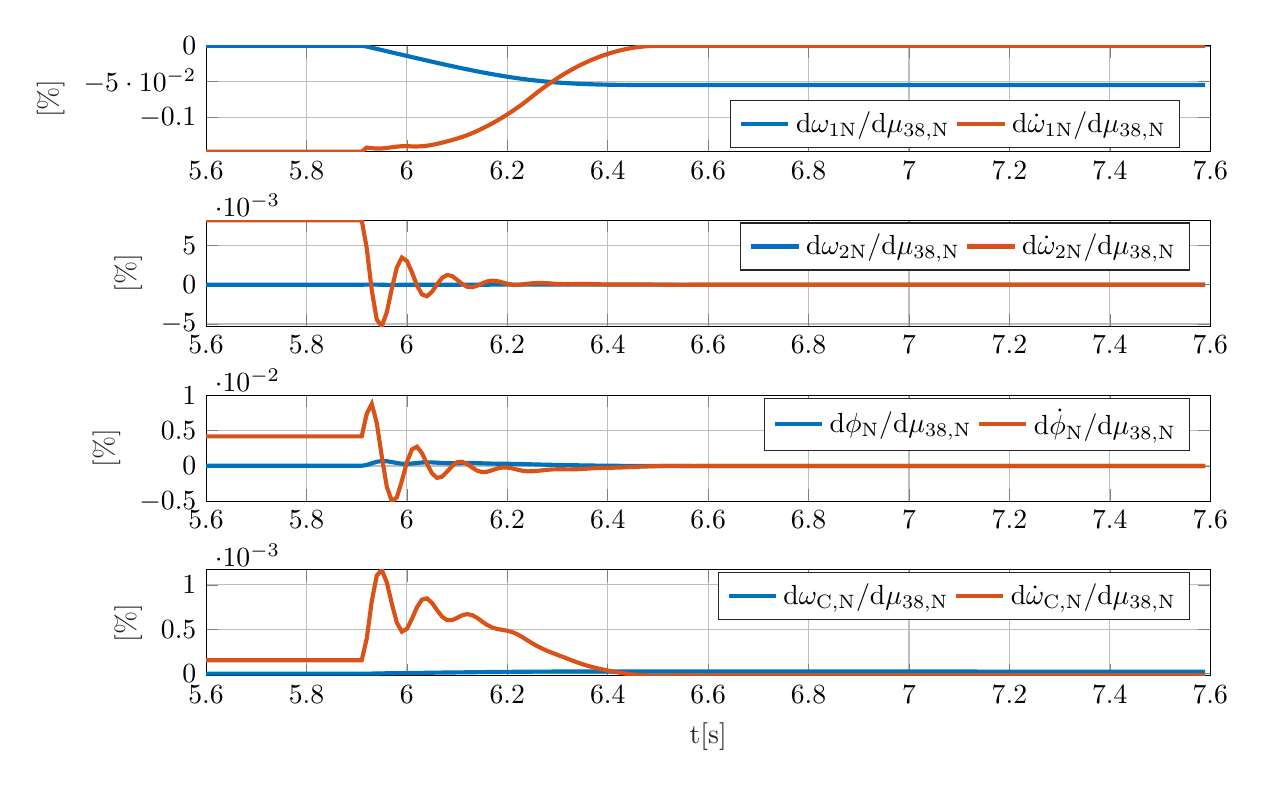
\begin{tikzpicture}

\begin{axis}[%
width=0.981\muwidth,
height=0.168\muheight,
at={(0\muwidth,0.832\muheight)},
scale only axis,
xmin=5.6,
xmax=7.6,
ymin=-0.147268813799723,
ymax=3.68664439137008e-06,
ylabel style={font=\color{white!15!black}},
ylabel={[$\%$]},
axis background/.style={fill=white},
xmajorgrids,
ymajorgrids,
legend style={at={(0.97,0.03)}, anchor=south east, legend columns=2, legend cell align=left, align=left, draw=white!15!black}
]
\addplot [color=mycolor1, line width=1.5pt]
  table[row sep=crcr]{%
5.59	0\\
5.6	0\\
5.61	0\\
5.62	0\\
5.63	0\\
5.64	0\\
5.65	0\\
5.66	0\\
5.67	0\\
5.68	0\\
5.69	0\\
5.7	0\\
5.71	0\\
5.72	0\\
5.73	0\\
5.74	0\\
5.75	0\\
5.76	0\\
5.77	0\\
5.78	0\\
5.79	0\\
5.8	0\\
5.81	0\\
5.82	0\\
5.83	0\\
5.84	0\\
5.85	0\\
5.86	0\\
5.87	0\\
5.88	0\\
5.89	0\\
5.9	0\\
5.91	0\\
5.92	-0.00101292552488464\\
5.93	-0.00264998214003995\\
5.94	-0.0042957939772962\\
5.95	-0.00594424158584209\\
5.96	-0.00758783939390802\\
5.97	-0.009221367419909\\
5.98	-0.0108436939860909\\
5.99	-0.0124572686091811\\
6	-0.0140663231134375\\
6.01	-0.0156755727343449\\
6.02	-0.0172902567132297\\
6.03	-0.0189035945740436\\
6.04	-0.0205109182149864\\
6.05	-0.0221073085196813\\
6.06	-0.0236887792708393\\
6.07	-0.0252523041628138\\
6.08	-0.0267960770477487\\
6.09	-0.0283188199784767\\
6.1	-0.0298190940044979\\
6.11	-0.031294837677735\\
6.12	-0.0327432698906522\\
6.13	-0.0341611564579983\\
6.14	-0.0355451631448896\\
6.15	-0.0368922186069717\\
6.16	-0.0381996594923875\\
6.17	-0.0394651674638322\\
6.18	-0.0406865542419889\\
6.19	-0.0418615718759464\\
6.2	-0.0429878612080495\\
6.21	-0.0440627325351002\\
6.22	-0.0450833610031978\\
6.23	-0.0460469059694538\\
6.24	-0.0469506814677504\\
6.25	-0.0477920501904116\\
6.26	-0.0485666659198021\\
6.27	-0.0492817850962357\\
6.28	-0.0499373519989886\\
6.29	-0.0505360368834669\\
6.3	-0.05108036822815\\
6.31	-0.0515729527810758\\
6.32	-0.0520163404112472\\
6.33	-0.0524130757450607\\
6.34	-0.0527657267882184\\
6.35	-0.0530768892088693\\
6.36	-0.0533491773563311\\
6.37	-0.0535852100448433\\
6.38	-0.0537875972852704\\
6.39	-0.0539589329030761\\
6.4	-0.0541017971522473\\
6.41	-0.0542188764779123\\
6.42	-0.0543126131189724\\
6.43	-0.054384388924997\\
6.44	-0.0544391336532811\\
6.45	-0.0544783537701355\\
6.46	-0.0545046188534428\\
6.47	-0.0545205312388944\\
6.48	-0.0545286829417293\\
6.49	-0.0545316612778472\\
6.5	-0.0545320508475198\\
6.51	-0.054532012249523\\
6.52	-0.0545319976549903\\
6.53	-0.0545320179030666\\
6.54	-0.0545320666453743\\
6.55	-0.0545321265963786\\
6.56	-0.0545321795860193\\
6.57	-0.0545322145554523\\
6.58	-0.0545322304674103\\
6.59	-0.0545322349442434\\
6.6	-0.0545322387725243\\
6.61	-0.0545322506538759\\
6.62	-0.0545322737860606\\
6.63	-0.054532305770409\\
6.64	-0.0545323409206814\\
6.65	-0.0545323734392977\\
6.66	-0.0545323999901063\\
6.67	-0.0545324205529309\\
6.68	-0.054532437708296\\
6.69	-0.054532454910007\\
6.7	-0.0545324748100065\\
6.71	-0.054532498287288\\
6.72	-0.0545325244642026\\
6.73	-0.0545325514886773\\
6.74	-0.0545325775533816\\
6.75	-0.054532601668421\\
6.76	-0.0545326238361712\\
6.77	-0.0545326451262249\\
6.78	-0.0545326665181444\\
6.79	-0.0545326887246664\\
6.8	-0.0545327119725904\\
6.81	-0.0545327359594364\\
6.82	-0.0545327601733071\\
6.83	-0.0545327841029649\\
6.84	-0.0545328074526622\\
6.85	-0.0545328302424194\\
6.86	-0.0545328527225088\\
6.87	-0.0545328752134728\\
6.88	-0.0545328979517867\\
6.89	-0.0545329210063182\\
6.9	-0.0545329442863711\\
6.91	-0.0545329676177616\\
6.92	-0.0545329908359722\\
6.93	-0.0545330138561913\\
6.94	-0.0545330366917368\\
6.95	-0.0545330594262724\\
6.96	-0.0545330821616895\\
6.97	-0.0545331049702716\\
6.98	-0.0545331278696139\\
6.99	-0.0545331508276122\\
7	-0.0545331737881438\\
7.01	-0.0545331967008654\\
7.02	-0.0545332195412114\\
7.03	-0.05453324231941\\
7.04	-0.0545332650600787\\
7.05	-0.05453328779376\\
7.06	-0.0545333105407007\\
7.07	-0.0545333333052734\\
7.08	-0.0545333560766367\\
7.09	-0.0545333788376103\\
7.1	-0.0545334015739284\\
7.11	-0.0545334242788354\\
7.12	-0.0545334469543159\\
7.13	-0.0545334696099493\\
7.14	-0.0545334922543372\\
7.15	-0.0545335148937483\\
7.16	-0.054533537529029\\
7.17	-0.0545335601564093\\
7.18	-0.0545335827705902\\
7.19	-0.0545336053672334\\
7.2	-0.0545336279447735\\
7.21	-0.0545336505038707\\
7.22	-0.0545336730470831\\
7.23	-0.0545336955774644\\
7.24	-0.054533718097195\\
7.25	-0.0545337406058029\\
7.26	-0.0545337631024192\\
7.27	-0.0545337855849462\\
7.28	-0.0545338080527774\\
7.29	-0.0545338305054692\\
7.3	-0.0545338529429584\\
7.31	-0.0545338753661001\\
7.32	-0.0545338977751554\\
7.33	-0.05453392017199\\
7.34	-0.0545339425559886\\
7.35	-0.0545339649267724\\
7.36	-0.0545339872832756\\
7.37	-0.0545340096253251\\
7.38	-0.0545340319536862\\
7.39	-0.0545340542679782\\
7.4	-0.0545340765683279\\
7.41	-0.054534098855011\\
7.42	-0.0545341211267224\\
7.43	-0.0545341433856054\\
7.44	-0.0545341656316936\\
7.45	-0.0545341878641106\\
7.46	-0.0545342100826732\\
7.47	-0.0545342322860993\\
7.48	-0.0545342544764601\\
7.49	-0.0545342766533868\\
7.5	-0.0545342988166074\\
7.51	-0.0545343209661651\\
7.52	-0.0545343431005389\\
7.53	-0.0545343652218008\\
7.54	-0.0545343873302734\\
7.55	-0.054534409424347\\
7.56	-0.0545344315045487\\
7.57	-0.0545344535709449\\
7.58	-0.0545344756244428\\
7.59	-0.054534497664233\\
};
\addlegendentry{d$\omega_{1\mathrm{N}}/$d$\mu_\mathrm{38,N}$}

\addplot [color=mycolor2, line width=1.5pt]
  table[row sep=crcr]{%
5.59	-0.147268813799723\\
5.6	-0.147268813799723\\
5.61	-0.147268813799723\\
5.62	-0.147268813799723\\
5.63	-0.147268813799723\\
5.64	-0.147268813799723\\
5.65	-0.147268813799723\\
5.66	-0.147268813799723\\
5.67	-0.147268813799723\\
5.68	-0.147268813799723\\
5.69	-0.147268813799723\\
5.7	-0.147268813799723\\
5.71	-0.147268813799723\\
5.72	-0.147268813799723\\
5.73	-0.147268813799723\\
5.74	-0.147268813799723\\
5.75	-0.147268813799723\\
5.76	-0.147268813799723\\
5.77	-0.147268813799723\\
5.78	-0.147268813799723\\
5.79	-0.147268813799723\\
5.8	-0.147268813799723\\
5.81	-0.147268813799723\\
5.82	-0.147268813799723\\
5.83	-0.147268813799723\\
5.84	-0.147268813799723\\
5.85	-0.147268813799723\\
5.86	-0.147268813799723\\
5.87	-0.147268813799723\\
5.88	-0.147268813799723\\
5.89	-0.147268813799723\\
5.9	-0.147268813799723\\
5.91	-0.147268813799723\\
5.92	-0.141511416774341\\
5.93	-0.142429931948264\\
5.94	-0.142974296682019\\
5.95	-0.142865166572011\\
5.96	-0.142166096947988\\
5.97	-0.141182512582358\\
5.98	-0.140275847466805\\
5.99	-0.139693938249168\\
6	-0.139494652220609\\
6.01	-0.140002952386445\\
6.02	-0.140048415852187\\
6.03	-0.139746833233327\\
6.04	-0.139012160522263\\
6.05	-0.137871308552401\\
6.06	-0.136422116619264\\
6.07	-0.134774478686145\\
6.08	-0.133003601858866\\
6.09	-0.13112392625891\\
6.1	-0.129096440958499\\
6.11	-0.126857650533195\\
6.12	-0.124352615463021\\
6.13	-0.121556829005585\\
6.14	-0.118479633396525\\
6.15	-0.115153192804553\\
6.16	-0.111612884328703\\
6.17	-0.107881463164687\\
6.18	-0.103962023999376\\
6.19	-0.0998407932568604\\
6.2	-0.0954983039214518\\
6.21	-0.0909171196072817\\
6.22	-0.0860897797020226\\
6.23	-0.0810201552059802\\
6.24	-0.0757185022116941\\
6.25	-0.0701962246465659\\
6.26	-0.0646825094695394\\
6.27	-0.059400794276633\\
6.28	-0.0543507175599783\\
6.29	-0.0495287331237715\\
6.3	-0.044930748876229\\
6.31	-0.0405536752670847\\
6.32	-0.0363967382637844\\
6.33	-0.0324613466527069\\
6.34	-0.0287499328213664\\
6.35	-0.0252646573735109\\
6.36	-0.0220065538944648\\
6.37	-0.018975371727913\\
6.38	-0.0161698819118526\\
6.39	-0.0135887007823562\\
6.4	-0.0112308978948057\\
6.41	-0.00909634165985997\\
6.42	-0.00718549753216364\\
6.43	-0.00549929543990294\\
6.44	-0.00403798764261352\\
6.45	-0.00280209832125945\\
6.46	-0.00179160985762162\\
6.47	-0.00100616003384784\\
6.48	-0.000445300436981938\\
6.49	-0.000108710540152761\\
6.5	3.68664439137008e-06\\
6.51	2.6096294159669e-06\\
6.52	-2.2161795320434e-07\\
6.53	-3.19966191742085e-06\\
6.54	-5.0152598343386e-06\\
6.55	-5.13214193336986e-06\\
6.56	-3.90475187843142e-06\\
6.57	-2.1431347269776e-06\\
6.58	-7.33681147604518e-07\\
6.59	-2.07041004168897e-07\\
6.6	-5.9120659443911e-07\\
6.61	-1.51660706474878e-06\\
6.62	-2.45765532790054e-06\\
6.63	-3.00308046694393e-06\\
6.64	-3.00537229473037e-06\\
6.65	-2.58595331889473e-06\\
6.66	-2.02084191180948e-06\\
6.67	-1.58678177854199e-06\\
6.68	-1.44171586193606e-06\\
6.69	-1.58222575717657e-06\\
6.7	-1.88257138256765e-06\\
6.71	-2.17601405042479e-06\\
6.72	-2.33646666256915e-06\\
6.73	-2.32399834810462e-06\\
6.74	-2.18226331840013e-06\\
6.75	-2.00206991766727e-06\\
6.76	-1.87460515914402e-06\\
6.77	-1.83761147985603e-06\\
6.78	-1.8816935737394e-06\\
6.79	-1.96989719441616e-06\\
6.8	-2.05376473089919e-06\\
6.81	-2.09874144896884e-06\\
6.82	-2.09426887089215e-06\\
6.83	-2.05221566489115e-06\\
6.84	-1.99856065568058e-06\\
6.85	-1.95858547180767e-06\\
6.86	-1.9458692808665e-06\\
6.87	-1.95915377704042e-06\\
6.88	-1.98621135779344e-06\\
6.89	-2.0115865168431e-06\\
6.9	-2.02411866508678e-06\\
6.91	-2.02064997185027e-06\\
6.92	-2.00571870648916e-06\\
6.93	-1.98779649799129e-06\\
6.94	-1.97473953598532e-06\\
6.95	-1.97052693525212e-06\\
6.96	-1.97442359784206e-06\\
6.97	-1.98235577944197e-06\\
6.98	-1.98940723106501e-06\\
6.99	-1.99221182104179e-06\\
7	-1.99002472783996e-06\\
7.01	-1.98442300867929e-06\\
7.02	-1.97817828299658e-06\\
7.03	-1.97357672101683e-06\\
7.04	-1.97167178577341e-06\\
7.05	-1.97217223090831e-06\\
7.06	-1.97375765343665e-06\\
7.07	-1.97497406961029e-06\\
7.08	-1.97487591574281e-06\\
7.09	-1.97326221712611e-06\\
7.1	-1.97068200863446e-06\\
7.11	-1.96793372234623e-06\\
7.12	-1.96574562352886e-06\\
7.13	-1.96439646833318e-06\\
7.14	-1.9637766239479e-06\\
7.15	-1.96346664658046e-06\\
7.16	-1.96299736749552e-06\\
7.17	-1.96209378781703e-06\\
7.18	-1.96073216844094e-06\\
7.19	-1.9590871451214e-06\\
7.2	-1.95741178865386e-06\\
7.21	-1.95591642768704e-06\\
7.22	-1.95469664383921e-06\\
7.23	-1.95369612550907e-06\\
7.24	-1.95277549786188e-06\\
7.25	-1.95179842980398e-06\\
7.26	-1.95068339741293e-06\\
7.27	-1.94942507531063e-06\\
7.28	-1.94808757765078e-06\\
7.29	-1.94674449442375e-06\\
7.3	-1.94545900803922e-06\\
7.31	-1.94425727020417e-06\\
7.32	-1.94312586232256e-06\\
7.33	-1.9420166756936e-06\\
7.34	-1.94089059229279e-06\\
7.35	-1.93972122734329e-06\\
7.36	-1.9385053535445e-06\\
7.37	-1.93726419528422e-06\\
7.38	-1.93602309721201e-06\\
7.39	-1.93480048196449e-06\\
7.4	-1.93360394668003e-06\\
7.41	-1.93242898161103e-06\\
7.42	-1.93126273630636e-06\\
7.43	-1.93009076496299e-06\\
7.44	-1.92890696307988e-06\\
7.45	-1.92771004412833e-06\\
7.46	-1.92650445828146e-06\\
7.47	-1.92529733508241e-06\\
7.48	-1.92409536366904e-06\\
7.49	-1.92290111933246e-06\\
7.5	-1.92171399170292e-06\\
7.51	-1.92053057889042e-06\\
7.52	-1.91934630860662e-06\\
7.53	-1.91815875322452e-06\\
7.54	-1.91696766861027e-06\\
7.55	-1.9157738110064e-06\\
7.56	-1.91457950526297e-06\\
7.57	-1.91338662457097e-06\\
7.58	-1.91219589676793e-06\\
7.59	-1.9110073622403e-06\\
};
\addlegendentry{d$\dot{\omega}_{1\mathrm{N}}/$d$\mu_\mathrm{38,N}$}

\end{axis}

\begin{axis}[%
width=0.981\muwidth,
height=0.168\muheight,
at={(0\muwidth,0.555\muheight)},
scale only axis,
xmin=5.6,
xmax=7.6,
ymin=-0.00526523819888062,
ymax=0.00818525653825591,
ylabel style={font=\color{white!15!black}},
ylabel={[$\%$]},
axis background/.style={fill=white},
xmajorgrids,
ymajorgrids,
legend style={legend columns=2, legend cell align=left, align=left, draw=white!15!black}
]
\addplot [color=mycolor1, line width=1.5pt]
  table[row sep=crcr]{%
5.59	0\\
5.6	0\\
5.61	0\\
5.62	0\\
5.63	0\\
5.64	0\\
5.65	0\\
5.66	0\\
5.67	0\\
5.68	0\\
5.69	0\\
5.7	0\\
5.71	0\\
5.72	0\\
5.73	0\\
5.74	0\\
5.75	0\\
5.76	0\\
5.77	0\\
5.78	0\\
5.79	0\\
5.8	0\\
5.81	0\\
5.82	0\\
5.83	0\\
5.84	0\\
5.85	0\\
5.86	0\\
5.87	0\\
5.88	0\\
5.89	0\\
5.9	0\\
5.91	0\\
5.92	9.51085508228791e-06\\
5.93	1.41148990560822e-05\\
5.94	7.28096234740413e-06\\
5.95	-5.26137215616256e-06\\
5.96	-1.64773044786499e-05\\
5.97	-2.14602332406319e-05\\
5.98	-1.91464214067401e-05\\
5.99	-1.18471898219661e-05\\
6	-3.67102745100737e-06\\
6.01	2.10581882634648e-06\\
6.02	3.90282202925132e-06\\
6.03	2.09732866230628e-06\\
6.04	-1.42533208598819e-06\\
6.05	-4.44664955006523e-06\\
6.06	-5.52395843329524e-06\\
6.07	-4.34548537662893e-06\\
6.08	-1.65164922334072e-06\\
6.09	1.32294402518787e-06\\
6.1	3.49502216143444e-06\\
6.11	4.36725218982352e-06\\
6.12	4.11359704142595e-06\\
6.13	3.34504889766267e-06\\
6.14	2.75600490584818e-06\\
6.15	2.79818759312764e-06\\
6.16	3.53919204750671e-06\\
6.17	4.72234196714601e-06\\
6.18	5.94475169096718e-06\\
6.19	6.87460235756457e-06\\
6.2	7.37191276514648e-06\\
6.21	7.4950025472953e-06\\
6.22	7.44572294078928e-06\\
6.23	7.44479265176365e-06\\
6.24	7.62720298668078e-06\\
6.25	8.00976764203428e-06\\
6.26	8.51577651033753e-06\\
6.27	9.0556068588369e-06\\
6.28	9.55377326761225e-06\\
6.29	9.9536096019774e-06\\
6.3	1.02416217333361e-05\\
6.31	1.04439038929841e-05\\
6.32	1.06084677602971e-05\\
6.33	1.07795547863644e-05\\
6.34	1.09791726620666e-05\\
6.35	1.12033163202237e-05\\
6.36	1.14304217459174e-05\\
6.37	1.16347280939216e-05\\
6.38	1.17987494100216e-05\\
6.39	1.19202134978902e-05\\
6.4	1.20096049142202e-05\\
6.41	1.20840923849303e-05\\
6.42	1.21569856932822e-05\\
6.43	1.22351696757427e-05\\
6.44	1.23177189203466e-05\\
6.45	1.24007335952736e-05\\
6.46	1.24767423779934e-05\\
6.47	1.25406165861395e-05\\
6.48	1.25917724358047e-05\\
6.49	1.26340457756046e-05\\
6.5	1.26734558064019e-05\\
6.51	1.27097366861169e-05\\
6.52	1.27234550790039e-05\\
6.53	1.27044225363196e-05\\
6.54	1.26586063294919e-05\\
6.55	1.26022543071003e-05\\
6.56	1.25524457434352e-05\\
6.57	1.25195755973209e-05\\
6.58	1.25046188668208e-05\\
6.59	1.25004107872334e-05\\
6.6	1.24968123259875e-05\\
6.61	1.24856442362704e-05\\
6.62	1.2463900724179e-05\\
6.63	1.24338364618395e-05\\
6.64	1.2400796332536e-05\\
6.65	1.23702298755896e-05\\
6.66	1.23452729666491e-05\\
6.67	1.23259445707043e-05\\
6.68	1.23098190773599e-05\\
6.69	1.2293650020505e-05\\
6.7	1.22749446588168e-05\\
6.71	1.22528767667287e-05\\
6.72	1.22282713061952e-05\\
6.73	1.22028691661606e-05\\
6.74	1.21783691796208e-05\\
6.75	1.21557018156034e-05\\
6.76	1.21348648410606e-05\\
6.77	1.21148528729754e-05\\
6.78	1.20947451543258e-05\\
6.79	1.20738717354526e-05\\
6.8	1.20520194320956e-05\\
6.81	1.2029472565739e-05\\
6.82	1.20067123035242e-05\\
6.83	1.19842191922319e-05\\
6.84	1.19622712251917e-05\\
6.85	1.19408495839674e-05\\
6.86	1.19197190204903e-05\\
6.87	1.18985782352398e-05\\
6.88	1.18772049490296e-05\\
6.89	1.18555344285202e-05\\
6.9	1.18336519249952e-05\\
6.91	1.18117211657737e-05\\
6.92	1.17898967920459e-05\\
6.93	1.17682585240468e-05\\
6.94	1.17467938432561e-05\\
6.95	1.17254241084841e-05\\
6.96	1.17040535452295e-05\\
6.97	1.16826142090777e-05\\
6.98	1.16610895613514e-05\\
6.99	1.1639509778906e-05\\
7	1.161792761514e-05\\
7.01	1.15963903913346e-05\\
7.02	1.15749211982002e-05\\
7.03	1.15535104217032e-05\\
7.04	1.15321349220254e-05\\
7.05	1.15107659903646e-05\\
7.06	1.14893845951963e-05\\
7.07	1.14679866266283e-05\\
7.08	1.14465822750593e-05\\
7.09	1.14251876894062e-05\\
7.1	1.14038162792606e-05\\
7.11	1.13824743944803e-05\\
7.12	1.13611601696442e-05\\
7.13	1.133986460044e-05\\
7.14	1.13185796017031e-05\\
7.15	1.12972992810417e-05\\
7.16	1.1276022842726e-05\\
7.17	1.12547538305231e-05\\
7.18	1.12334972253609e-05\\
7.19	1.12122571050902e-05\\
7.2	1.11910349411116e-05\\
7.21	1.11698301129349e-05\\
7.22	1.11486402158992e-05\\
7.23	1.11274623796473e-05\\
7.24	1.11062945547582e-05\\
7.25	1.10851371848831e-05\\
7.26	1.10639910867128e-05\\
7.27	1.10428582319463e-05\\
7.28	1.10217391908871e-05\\
7.29	1.10006343802494e-05\\
7.3	1.09795438597052e-05\\
7.31	1.09584668252596e-05\\
7.32	1.09374030316089e-05\\
7.33	1.09163507249797e-05\\
7.34	1.0895310483804e-05\\
7.35	1.08742826641815e-05\\
7.36	1.08532682677337e-05\\
7.37	1.08322674573639e-05\\
7.38	1.08112795136717e-05\\
7.39	1.07903047945309e-05\\
7.4	1.07693431806886e-05\\
7.41	1.07483944129106e-05\\
7.42	1.07274597181121e-05\\
7.43	1.07065370815859e-05\\
7.44	1.06856264718422e-05\\
7.45	1.06647287124626e-05\\
7.46	1.06438439757931e-05\\
7.47	1.06229734669759e-05\\
7.48	1.06021152390827e-05\\
7.49	1.05812696389031e-05\\
7.5	1.05604369219307e-05\\
7.51	1.05396170476681e-05\\
7.52	1.05188114458849e-05\\
7.53	1.0498018168754e-05\\
7.54	1.04772369132118e-05\\
7.55	1.04564691922465e-05\\
7.56	1.04357145104211e-05\\
7.57	1.04149728053526e-05\\
7.58	1.03942432242164e-05\\
7.59	1.03735265278797e-05\\
};
\addlegendentry{d$\omega_{2\mathrm{N}}/$d$\mu_\mathrm{38,N}$}

\addplot [color=mycolor2, line width=1.5pt]
  table[row sep=crcr]{%
5.59	0.00818525653825591\\
5.6	0.00818525653825591\\
5.61	0.00818525653825591\\
5.62	0.00818525653825591\\
5.63	0.00818525653825591\\
5.64	0.00818525653825591\\
5.65	0.00818525653825591\\
5.66	0.00818525653825591\\
5.67	0.00818525653825591\\
5.68	0.00818525653825591\\
5.69	0.00818525653825591\\
5.7	0.00818525653825591\\
5.71	0.00818525653825591\\
5.72	0.00818525653825591\\
5.73	0.00818525653825591\\
5.74	0.00818525653825591\\
5.75	0.00818525653825591\\
5.76	0.00818525653825591\\
5.77	0.00818525653825591\\
5.78	0.00818525653825591\\
5.79	0.00818525653825591\\
5.8	0.00818525653825591\\
5.81	0.00818525653825591\\
5.82	0.00818525653825591\\
5.83	0.00818525653825591\\
5.84	0.00818525653825591\\
5.85	0.00818525653825591\\
5.86	0.00818525653825591\\
5.87	0.00818525653825591\\
5.88	0.00818525653825591\\
5.89	0.00818525653825591\\
5.9	0.00818525653825591\\
5.91	0.00818525653825591\\
5.92	0.0046419820074494\\
5.93	-0.000719255674786555\\
5.94	-0.00443193823933017\\
5.95	-0.00526523819888062\\
5.96	-0.0034991885371333\\
5.97	-0.000479530211649873\\
5.98	0.00220121197275262\\
5.99	0.00345103776622961\\
6	0.00301497641703718\\
6.01	0.00159431315989547\\
6.02	-9.15100685816105e-05\\
6.03	-0.00123854035543223\\
6.04	-0.00146765670051584\\
6.05	-0.000897431708245516\\
6.06	4.10420606528269e-05\\
6.07	0.000863557623809651\\
6.08	0.00123874276865753\\
6.09	0.00110297245667148\\
6.1	0.000628133869388181\\
6.11	9.39960399919077e-05\\
6.12	-0.000257370417409112\\
6.13	-0.000317985633624376\\
6.14	-0.000129012704340283\\
6.15	0.000167828892804737\\
6.16	0.000416663094609656\\
6.17	0.000517227572552659\\
6.18	0.00045588673696441\\
6.19	0.000293328740566504\\
6.2	0.000115327766401623\\
6.21	-1.28921950004672e-06\\
6.22	-2.36497965477332e-05\\
6.23	3.11899084174773e-05\\
6.24	0.000118040228280319\\
6.25	0.000186653987407563\\
6.26	0.000217540759703843\\
6.27	0.000216542554009561\\
6.28	0.00018525222064486\\
6.29	0.000139294755900672\\
6.3	9.6700444196362e-05\\
6.31	7.10822426613962e-05\\
6.32	6.58506386106653e-05\\
6.33	7.47983374739185e-05\\
6.34	8.72079260023454e-05\\
6.35	9.35595052882968e-05\\
6.36	8.92989650273907e-05\\
6.37	7.55307292860627e-05\\
6.38	5.76697632272429e-05\\
6.39	4.18126686539849e-05\\
6.4	3.2059104615886e-05\\
6.41	2.89888707283844e-05\\
6.42	3.05511137673973e-05\\
6.43	3.26484501518587e-05\\
6.44	3.41693918155999e-05\\
6.45	3.28043297961346e-05\\
6.46	2.86308922394167e-05\\
6.47	2.32450577404675e-05\\
6.48	1.86225916448913e-05\\
6.49	1.61757767063418e-05\\
6.5	1.62438308926595e-05\\
6.51	1.14983639389538e-05\\
6.52	-9.76477298177919e-07\\
6.53	-1.40981232749037e-05\\
6.54	-2.20978819715969e-05\\
6.55	-2.26128795817504e-05\\
6.56	-1.72048406240404e-05\\
6.57	-9.44292814536255e-06\\
6.58	-3.23269380651951e-06\\
6.59	-9.12249379798781e-07\\
6.6	-2.60493254114098e-06\\
6.61	-6.68236642190415e-06\\
6.62	-1.08287464970345e-05\\
6.63	-1.32319600383149e-05\\
6.64	-1.32420581272672e-05\\
6.65	-1.13940440002212e-05\\
6.66	-8.9040902217403e-06\\
6.67	-6.99156526583543e-06\\
6.68	-6.35238611876315e-06\\
6.69	-6.97149084781523e-06\\
6.7	-8.29485242823357e-06\\
6.71	-9.58779868703716e-06\\
6.72	-1.02947736000665e-05\\
6.73	-1.02398365976934e-05\\
6.74	-9.61533376810748e-06\\
6.75	-8.82137839331474e-06\\
6.76	-8.25975221991145e-06\\
6.77	-8.09675329550787e-06\\
6.78	-8.29098468926903e-06\\
6.79	-8.67962122327995e-06\\
6.8	-9.04915241082894e-06\\
6.81	-9.2473256341919e-06\\
6.82	-9.2276188780688e-06\\
6.83	-9.04232702611441e-06\\
6.84	-8.80591613218601e-06\\
6.85	-8.62978031386445e-06\\
6.86	-8.5737511357501e-06\\
6.87	-8.63228434005092e-06\\
6.88	-8.75150353220972e-06\\
6.89	-8.86330975725321e-06\\
6.9	-8.91852801949431e-06\\
6.91	-8.90324450951319e-06\\
6.92	-8.83745542768408e-06\\
6.93	-8.75848786445936e-06\\
6.94	-8.7009572050624e-06\\
6.95	-8.68239594266119e-06\\
6.96	-8.69956514083629e-06\\
6.97	-8.73451535649067e-06\\
6.98	-8.76558496222281e-06\\
6.99	-8.7779423475484e-06\\
7	-8.76830573269114e-06\\
7.01	-8.74362383525404e-06\\
7.02	-8.71610876811102e-06\\
7.03	-8.69583369226843e-06\\
7.04	-8.68744030178354e-06\\
7.05	-8.68964532762207e-06\\
7.06	-8.69663090385667e-06\\
7.07	-8.70199059047708e-06\\
7.08	-8.70155811187193e-06\\
7.09	-8.69444794754332e-06\\
7.1	-8.68307921599333e-06\\
7.11	-8.6709699119841e-06\\
7.12	-8.66132886625428e-06\\
7.13	-8.65538431437484e-06\\
7.14	-8.65265320003183e-06\\
7.15	-8.6512873997533e-06\\
7.16	-8.64921969555191e-06\\
7.17	-8.64523840689541e-06\\
7.18	-8.63923893622841e-06\\
7.19	-8.63199075121785e-06\\
7.2	-8.62460891444268e-06\\
7.21	-8.61802016107019e-06\\
7.22	-8.61264563604266e-06\\
7.23	-8.60823722317852e-06\\
7.24	-8.60418081897226e-06\\
7.25	-8.59987573103344e-06\\
7.26	-8.5949627544414e-06\\
7.27	-8.58941842489102e-06\\
7.28	-8.58352523761855e-06\\
7.29	-8.57760743961654e-06\\
7.3	-8.57194342073409e-06\\
7.31	-8.56664840876712e-06\\
7.32	-8.56166327965029e-06\\
7.33	-8.55677606023919e-06\\
7.34	-8.5518143914719e-06\\
7.35	-8.54666201861611e-06\\
7.36	-8.54130472176886e-06\\
7.37	-8.5358360183219e-06\\
7.38	-8.53036758007123e-06\\
7.39	-8.52498057953144e-06\\
7.4	-8.5197084906736e-06\\
7.41	-8.51453144296868e-06\\
7.42	-8.50939281567027e-06\\
7.43	-8.50422895870683e-06\\
7.44	-8.49901297485911e-06\\
7.45	-8.4937391955144e-06\\
7.46	-8.48842722871068e-06\\
7.47	-8.48310848813536e-06\\
7.48	-8.47781244699212e-06\\
7.49	-8.47255045234639e-06\\
7.5	-8.46731981483031e-06\\
7.51	-8.46210554527727e-06\\
7.52	-8.45688749759529e-06\\
7.53	-8.45165497534648e-06\\
7.54	-8.44640690284451e-06\\
7.55	-8.44114661219317e-06\\
7.56	-8.43588434698123e-06\\
7.57	-8.43062836072924e-06\\
7.58	-8.4253818603842e-06\\
7.59	-8.42014502389377e-06\\
};
\addlegendentry{d$\dot{\omega}_{2\mathrm{N}}/$d$\mu_\mathrm{38,N}$}

\end{axis}

\begin{axis}[%
width=0.981\muwidth,
height=0.168\muheight,
at={(0\muwidth,0.277\muheight)},
scale only axis,
xmin=5.6,
xmax=7.6,
ymin=-0.00499672753981617,
ymax=0.01,
ylabel style={font=\color{white!15!black}},
ylabel={[$\%$]},
axis background/.style={fill=white},
xmajorgrids,
ymajorgrids,
legend style={legend columns=2, legend cell align=left, align=left, draw=white!15!black}
]
\addplot [color=mycolor1, line width=1.5pt]
  table[row sep=crcr]{%
5.59	3.40496496175267e-05\\
5.6	3.40496496175267e-05\\
5.61	3.40496496175267e-05\\
5.62	3.40496496175267e-05\\
5.63	3.40496496175267e-05\\
5.64	3.40496496175267e-05\\
5.65	3.40496496175267e-05\\
5.66	3.40496496175267e-05\\
5.67	3.40496496175267e-05\\
5.68	3.40496496175267e-05\\
5.69	3.40496496175267e-05\\
5.7	3.40496496175267e-05\\
5.71	3.40496496175267e-05\\
5.72	3.40496496175267e-05\\
5.73	3.40496496175267e-05\\
5.74	3.40496496175267e-05\\
5.75	3.40496496175267e-05\\
5.76	3.40496496175267e-05\\
5.77	3.40496496175267e-05\\
5.78	3.40496496175267e-05\\
5.79	3.40496496175267e-05\\
5.8	3.40496496175267e-05\\
5.81	3.40496496175267e-05\\
5.82	3.40496496175267e-05\\
5.83	3.40496496175267e-05\\
5.84	3.40496496175267e-05\\
5.85	3.40496496175267e-05\\
5.86	3.40496496175267e-05\\
5.87	3.40496496175267e-05\\
5.88	3.40496496175267e-05\\
5.89	3.40496496175267e-05\\
5.9	3.40496496175267e-05\\
5.91	3.40496496175267e-05\\
5.92	0.000138665456178876\\
5.93	0.000378159917094936\\
5.94	0.000595414040010772\\
5.95	0.000701883406176927\\
5.96	0.000675669927399545\\
5.97	0.00055725823544345\\
5.98	0.00041847022568014\\
5.99	0.000323886236770731\\
6	0.000306579197285364\\
6.01	0.000350672851757537\\
6.02	0.000425966153802699\\
6.03	0.000492556017955775\\
6.04	0.000522555087484792\\
6.05	0.000510518229106811\\
6.06	0.000470059514894446\\
6.07	0.000423068835852961\\
6.08	0.000389334175650193\\
6.09	0.000378158307566074\\
6.1	0.000386666314481014\\
6.11	0.000403800146188948\\
6.12	0.000416944109464474\\
6.13	0.000417777995280646\\
6.14	0.000404789593937627\\
6.15	0.00038256401400839\\
6.16	0.000358309329463154\\
6.17	0.000338173196898792\\
6.18	0.000324841862999483\\
6.19	0.000317041013915692\\
6.2	0.000311313427316832\\
6.21	0.000303635394844575\\
6.22	0.000291389905157177\\
6.23	0.000274284733123806\\
6.24	0.00025382361314137\\
6.25	0.00023235110162282\\
6.26	0.000211926804486533\\
6.27	0.000193475005057881\\
6.28	0.00017729884983454\\
6.29	0.000162932998231454\\
6.3	0.000149577617476354\\
6.31	0.000136447642534504\\
6.32	0.000123141898070388\\
6.33	0.000109744339452601\\
6.34	9.66696154974435e-05\\
6.35	8.4405489623141e-05\\
6.36	7.32875762759645e-05\\
6.37	6.33983916333429e-05\\
6.38	5.45698025410554e-05\\
6.39	4.65239232026706e-05\\
6.4	3.90153274204259e-05\\
6.41	3.19357468648634e-05\\
6.42	2.53232786625084e-05\\
6.43	1.93450963320165e-05\\
6.44	1.40713449484726e-05\\
6.45	9.63717928305068e-06\\
6.46	6.08254456912019e-06\\
6.47	3.36206049927802e-06\\
6.48	1.38900513148563e-06\\
6.49	8.16770082893438e-08\\
6.5	-6.00631701259814e-07\\
6.51	-6.65567300863172e-07\\
6.52	-2.42051033265634e-07\\
6.53	3.78015889096166e-07\\
6.54	8.85076155845098e-07\\
6.55	1.08243783210792e-06\\
6.56	9.59799916688871e-07\\
6.57	6.37738337782038e-07\\
6.58	3.00629293331875e-07\\
6.59	9.79213712910405e-08\\
6.6	8.6715756066125e-08\\
6.61	2.29331206119022e-07\\
6.62	4.28683362200626e-07\\
6.63	5.85576365857404e-07\\
6.64	6.41559986101825e-07\\
6.65	5.95087739481156e-07\\
6.66	4.89293433428339e-07\\
6.67	3.83181713441721e-07\\
6.68	3.2271286145044e-07\\
6.69	3.23526799622084e-07\\
6.7	3.71340859655667e-07\\
6.71	4.34714154099491e-07\\
6.72	4.82561527067838e-07\\
6.73	4.97578514489812e-07\\
6.74	4.80522566296279e-07\\
6.75	4.46095266408847e-07\\
6.76	4.13787855777896e-07\\
6.77	3.96722850977826e-07\\
6.78	3.9753620165884e-07\\
6.79	4.11716677668763e-07\\
6.8	4.29992078300332e-07\\
6.81	4.43546715483152e-07\\
6.82	4.47699941355725e-07\\
6.83	4.42563091900574e-07\\
6.84	4.32281230516955e-07\\
6.85	4.22347140137204e-07\\
6.86	4.16845883966075e-07\\
6.87	4.17027086156192e-07\\
6.88	4.21399474754361e-07\\
6.89	4.26988086886199e-07\\
6.9	4.30978877083813e-07\\
6.91	4.31871088737853e-07\\
6.92	4.29853283500716e-07\\
6.93	4.26331771195502e-07\\
6.94	4.23046537468198e-07\\
6.95	4.21243035380208e-07\\
6.96	4.21246392949874e-07\\
6.97	4.22528579575675e-07\\
6.98	4.24122032667405e-07\\
6.99	4.25153599087533e-07\\
7	4.251962565876e-07\\
7.01	4.24347142878298e-07\\
7.02	4.23081979456083e-07\\
7.03	4.21935393201842e-07\\
7.04	4.21251251703219e-07\\
7.05	4.21114670923336e-07\\
7.06	4.21338902334884e-07\\
7.07	4.21636218451054e-07\\
7.08	4.2175083092111e-07\\
7.09	4.21559386631912e-07\\
7.1	4.21109401877793e-07\\
7.11	4.20539516528426e-07\\
7.12	4.20015674867644e-07\\
7.13	4.19640720593463e-07\\
7.14	4.19433562844913e-07\\
7.15	4.19336689967514e-07\\
7.16	4.19251435256809e-07\\
7.17	4.1910232540791e-07\\
7.18	4.18858624952701e-07\\
7.19	4.1853679621856e-07\\
7.2	4.18182520430682e-07\\
7.21	4.17844535057598e-07\\
7.22	4.17556450022917e-07\\
7.23	4.17320558718525e-07\\
7.24	4.17115041698099e-07\\
7.25	4.16911995163936e-07\\
7.26	4.1668781112174e-07\\
7.27	4.16433425431868e-07\\
7.28	4.16156418075728e-07\\
7.29	4.15870356739737e-07\\
7.3	4.15589910511081e-07\\
7.31	4.1532465158773e-07\\
7.32	4.15076301298049e-07\\
7.33	4.14836776698635e-07\\
7.34	4.14598037772948e-07\\
7.35	4.14352786881384e-07\\
7.36	4.14097715605418e-07\\
7.37	4.13835278862659e-07\\
7.38	4.13570392534285e-07\\
7.39	4.13307425093476e-07\\
7.4	4.13049207736334e-07\\
7.41	4.12796050966237e-07\\
7.42	4.12546207010147e-07\\
7.43	4.12296398711526e-07\\
7.44	4.1204483575157e-07\\
7.45	4.11790606873673e-07\\
7.46	4.11534071852981e-07\\
7.47	4.11276397789662e-07\\
7.48	4.11019211515927e-07\\
7.49	4.10763373728225e-07\\
7.5	4.1050912627349e-07\\
7.51	4.10256027231224e-07\\
7.52	4.10003201234569e-07\\
7.53	4.09749920716347e-07\\
7.54	4.09495950081216e-07\\
7.55	4.09241271766778e-07\\
7.56	4.08986283663072e-07\\
7.57	4.08731408366647e-07\\
7.58	4.08476899406559e-07\\
7.59	4.08222859253567e-07\\
};
\addlegendentry{d$\phi_\mathrm{N}/$d$\mu_\mathrm{38,N}$}

\addplot [color=mycolor2, line width=1.5pt]
  table[row sep=crcr]{%
5.59	0.00419533692567792\\
5.6	0.00419533692567792\\
5.61	0.00419533692567792\\
5.62	0.00419533692567792\\
5.63	0.00419533692567792\\
5.64	0.00419533692567792\\
5.65	0.00419533692567792\\
5.66	0.00419533692567792\\
5.67	0.00419533692567792\\
5.68	0.00419533692567792\\
5.69	0.00419533692567792\\
5.7	0.00419533692567792\\
5.71	0.00419533692567792\\
5.72	0.00419533692567792\\
5.73	0.00419533692567792\\
5.74	0.00419533692567792\\
5.75	0.00419533692567792\\
5.76	0.00419533692567792\\
5.77	0.00419533692567792\\
5.78	0.00419533692567792\\
5.79	0.00419533692567792\\
5.8	0.00419533692567792\\
5.81	0.00419533692567792\\
5.82	0.00419533692567792\\
5.83	0.00419533692567792\\
5.84	0.00419533692567792\\
5.85	0.00419533692567792\\
5.86	0.00419533692567792\\
5.87	0.00419533692567792\\
5.88	0.00419533692567792\\
5.89	0.00419533692567792\\
5.9	0.00419533692567792\\
5.91	0.00419533692567792\\
5.92	0.007423650804719\\
5.93	0.00879605507892209\\
5.94	0.0060824589680548\\
5.95	0.00133015682739307\\
5.96	-0.00294727267142762\\
5.97	-0.00499672753981617\\
5.98	-0.00443820568832031\\
5.99	-0.00209761424185419\\
6	0.000557068654949401\\
6.01	0.00235502052415382\\
6.02	0.00273096508280751\\
6.03	0.00182082947791144\\
6.04	0.000298720006816753\\
6.05	-0.00104225455600327\\
6.06	-0.00168623611260551\\
6.07	-0.00152140204567619\\
6.08	-0.000811898335636489\\
6.09	1.5644370852847e-06\\
6.1	0.000532359964132868\\
6.11	0.000603227827148173\\
6.12	0.00027676590309508\\
6.13	-0.000228282781835972\\
6.14	-0.000663379924811655\\
6.15	-0.00086670312357433\\
6.16	-0.000813682923943005\\
6.17	-0.000595612354791143\\
6.18	-0.000356018130964778\\
6.19	-0.000213033466948132\\
6.2	-0.000216260652951639\\
6.21	-0.000344428712848075\\
6.22	-0.000524987100010958\\
6.23	-0.000678647381604916\\
6.24	-0.000756764380148021\\
6.25	-0.000752906865274053\\
6.26	-0.000693755042086661\\
6.27	-0.000612540858215117\\
6.28	-0.000536217283955785\\
6.29	-0.000485473143935559\\
6.3	-0.0004655548105612\\
6.31	-0.000467583629143538\\
6.32	-0.000474844103735288\\
6.33	-0.000471966403951417\\
6.34	-0.000451524811000745\\
6.35	-0.000415387739713721\\
6.36	-0.000371696933067741\\
6.37	-0.00033009303698147\\
6.38	-0.000297259392041466\\
6.39	-0.000274442916398246\\
6.4	-0.000258332153191832\\
6.41	-0.000243246100324783\\
6.42	-0.000224840723705216\\
6.43	-0.000200889978768286\\
6.44	-0.000172547181576433\\
6.45	-0.000141457504734642\\
6.46	-0.000110718254599845\\
6.47	-8.25950585133408e-05\\
6.48	-5.77282968934887e-05\\
6.49	-3.51788138279966e-05\\
6.5	-1.32269408963598e-05\\
6.51	7.67321470748907e-06\\
6.52	2.0506522658521e-05\\
6.53	2.16329010725891e-05\\
6.54	1.31760321233932e-05\\
6.55	9.58931983389878e-07\\
6.56	-8.92460572746409e-06\\
6.57	-1.27606334626181e-05\\
6.58	-1.02010177797849e-05\\
6.59	-3.80595742087741e-06\\
6.6	2.80172499539459e-06\\
6.61	6.69954018451497e-06\\
6.62	6.8135509733017e-06\\
6.63	3.94940465294965e-06\\
6.64	1.68503419433713e-08\\
6.65	-3.03702620160893e-06\\
6.66	-4.09186393811843e-06\\
6.67	-3.14100019524138e-06\\
6.68	-1.05121371467066e-06\\
6.69	1.01745334356241e-06\\
6.7	2.17429787750359e-06\\
6.71	2.12408614562772e-06\\
6.72	1.16155913434413e-06\\
6.73	-9.12921502245797e-08\\
6.74	-1.02752155806377e-06\\
6.75	-1.31473657471274e-06\\
6.76	-9.54229665949002e-07\\
6.77	-3.04759031027562e-07\\
6.78	3.04700931124307e-07\\
6.79	6.34603896504315e-07\\
6.8	6.08704872250448e-07\\
6.81	3.28801660437514e-07\\
6.82	-3.31973746077844e-08\\
6.83	-3.05572578242893e-07\\
6.84	-3.8892132896955e-07\\
6.85	-2.89896844616688e-07\\
6.86	-9.24895224342628e-08\\
6.87	9.57049408899777e-08\\
6.88	1.95323226243707e-07\\
6.89	1.83294548719405e-07\\
6.9	9.01401187004265e-08\\
6.91	-2.55777618335911e-08\\
6.92	-1.08543420406132e-07\\
6.93	-1.30212174096312e-07\\
6.94	-9.49985108746926e-08\\
6.95	-3.09442904275587e-08\\
6.96	2.77862481249057e-08\\
6.97	5.69633316734801e-08\\
6.98	5.07546047267795e-08\\
6.99	2.00954925147522e-08\\
7	-1.60248346953824e-08\\
7.01	-4.06242486680814e-08\\
7.02	-4.54712790282334e-08\\
7.03	-3.38550779170124e-08\\
7.04	-1.42014301187574e-08\\
7.05	3.05053462014456e-09\\
7.06	1.11528571425635e-08\\
7.07	8.491888385694e-09\\
7.08	-1.11540661089684e-09\\
7.09	-1.19690676846037e-08\\
7.1	-1.91277173892683e-08\\
7.11	-2.0333235698099e-08\\
7.12	-1.63242484501819e-08\\
7.13	-1.01702596241503e-08\\
7.14	-4.87033206592985e-09\\
7.15	-2.69641862323785e-09\\
7.16	-3.75654187483743e-09\\
7.17	-6.86392084140286e-09\\
7.18	-1.01997554713588e-08\\
7.19	-1.22878608819823e-08\\
7.2	-1.25356641578965e-08\\
7.21	-1.12139906739398e-08\\
7.22	-9.25813874252445e-09\\
7.23	-7.68279527932794e-09\\
7.24	-7.05091101880658e-09\\
7.25	-7.44821261022219e-09\\
7.26	-8.43544475571927e-09\\
7.27	-9.45087341257199e-09\\
7.28	-1.00614041830052e-08\\
7.29	-1.01148583355648e-08\\
7.3	-9.69460571766123e-09\\
7.31	-9.0832172330149e-09\\
7.32	-8.6057380732768e-09\\
7.33	-8.41740895992515e-09\\
7.34	-8.54045605978125e-09\\
7.35	-8.8570203791726e-09\\
7.36	-9.18149232148586e-09\\
7.37	-9.36664760039512e-09\\
7.38	-9.37730402512219e-09\\
7.39	-9.2442390672108e-09\\
7.4	-9.05311525655912e-09\\
7.41	-8.89418250577323e-09\\
7.42	-8.83805299277053e-09\\
7.43	-8.87110286700732e-09\\
7.44	-8.95884239348336e-09\\
7.45	-9.05616519421831e-09\\
7.46	-9.12122167720731e-09\\
7.47	-9.1288256286022e-09\\
7.48	-9.09303408262679e-09\\
7.49	-9.03586757531901e-09\\
7.5	-8.98370117481585e-09\\
7.51	-8.95669956256243e-09\\
7.52	-8.96202329278393e-09\\
7.53	-8.98485132329539e-09\\
7.54	-9.01218286368091e-09\\
7.55	-9.03132909327906e-09\\
7.56	-9.03530407090238e-09\\
7.57	-9.02570764691533e-09\\
7.58	-9.00949154768783e-09\\
7.59	-8.99330611594403e-09\\
};
\addlegendentry{d$\dot{\phi}_\mathrm{N}/$d$\mu_\mathrm{38,N}$}

\end{axis}

\begin{axis}[%
width=0.981\muwidth,
height=0.168\muheight,
at={(0\muwidth,0\muheight)},
scale only axis,
xmin=5.6,
xmax=7.6,
xlabel style={font=\color{white!15!black}},
xlabel={t[s]},
ymin=-2.34231476506925e-05,
ymax=0.00116908956267171,
ylabel style={font=\color{white!15!black}},
ylabel={[$\%$]},
axis background/.style={fill=white},
xmajorgrids,
ymajorgrids,
legend style={legend columns=2, legend cell align=left, align=left, draw=white!15!black}
]
\addplot [color=mycolor1, line width=1.5pt]
  table[row sep=crcr]{%
5.59	0\\
5.6	0\\
5.61	0\\
5.62	0\\
5.63	0\\
5.64	0\\
5.65	0\\
5.66	0\\
5.67	0\\
5.68	0\\
5.69	0\\
5.7	0\\
5.71	0\\
5.72	0\\
5.73	0\\
5.74	0\\
5.75	0\\
5.76	0\\
5.77	0\\
5.78	0\\
5.79	0\\
5.8	0\\
5.81	0\\
5.82	0\\
5.83	0\\
5.84	0\\
5.85	0\\
5.86	0\\
5.87	0\\
5.88	0\\
5.89	0\\
5.9	0\\
5.91	0\\
5.92	1.75478401952086e-07\\
5.93	8.10917326373928e-07\\
5.94	1.82394332184804e-06\\
5.95	3.02393787787438e-06\\
5.96	4.17713603484769e-06\\
5.97	5.12065963501798e-06\\
5.98	5.81938619065396e-06\\
5.99	6.35028675219732e-06\\
6	6.84985365922615e-06\\
6.01	7.42753044665488e-06\\
6.02	8.13741069779737e-06\\
6.03	8.96377769619708e-06\\
6.04	9.84263417173481e-06\\
6.05	1.06990425257466e-05\\
6.06	1.14839510313004e-05\\
6.07	1.21857733779347e-05\\
6.08	1.28279268496941e-05\\
6.09	1.34502169026584e-05\\
6.1	1.40873862321834e-05\\
6.11	1.47546892791032e-05\\
6.12	1.54450734556546e-05\\
6.13	1.61369874221073e-05\\
6.14	1.6806125216579e-05\\
6.15	1.74362643341789e-05\\
6.16	1.80239518832781e-05\\
6.17	1.85765054058892e-05\\
6.18	1.9106078262864e-05\\
6.19	1.9622459729737e-05\\
6.2	2.01291045187769e-05\\
6.21	2.06228225576676e-05\\
6.22	2.10956692336784e-05\\
6.23	2.15390833252651e-05\\
6.24	2.19473879162173e-05\\
6.25	2.23187993822503e-05\\
6.26	2.26537592811718e-05\\
6.27	2.29587423726366e-05\\
6.28	2.3236203671387e-05\\
6.29	2.34893033297876e-05\\
6.3	2.37197182629453e-05\\
6.31	2.39278681271449e-05\\
6.32	2.41134280785121e-05\\
6.33	2.427619433247e-05\\
6.34	2.44167014881414e-05\\
6.35	2.45363474157731e-05\\
6.36	2.46371117443866e-05\\
6.37	2.47211116798353e-05\\
6.38	2.47901876209195e-05\\
6.39	2.48456731145235e-05\\
6.4	2.48884769177781e-05\\
6.41	2.49193398966569e-05\\
6.42	2.49390101106581e-05\\
6.43	2.49479353022788e-05\\
6.44	2.4948525136615e-05\\
6.45	2.49416371630111e-05\\
6.46	2.49287566060663e-05\\
6.47	2.49113063480262e-05\\
6.48	2.48905544110517e-05\\
6.49	2.48676208735145e-05\\
6.5	2.48435521426408e-05\\
6.51	2.48193955315588e-05\\
6.52	2.47960034959019e-05\\
6.53	2.47737136833781e-05\\
6.54	2.47523522719657e-05\\
6.55	2.47313285795068e-05\\
6.56	2.47101003374073e-05\\
6.57	2.4688322809249e-05\\
6.58	2.46659642887686e-05\\
6.59	2.46432633883776e-05\\
6.6	2.46205572630035e-05\\
6.61	2.45981176856395e-05\\
6.62	2.45760443876507e-05\\
6.63	2.45542623350282e-05\\
6.64	2.45325939519286e-05\\
6.65	2.451085835145e-05\\
6.66	2.44889516391654e-05\\
6.67	2.44668735134852e-05\\
6.68	2.4444704845169e-05\\
6.69	2.4422553684861e-05\\
6.7	2.44005029549364e-05\\
6.71	2.43785801630521e-05\\
6.72	2.43567579628491e-05\\
6.73	2.43349786196333e-05\\
6.74	2.43131858482689e-05\\
6.75	2.42913489318057e-05\\
6.76	2.42694693746509e-05\\
6.77	2.424757922193e-05\\
6.78	2.42257090183675e-05\\
6.79	2.42038815151279e-05\\
6.8	2.41821040070991e-05\\
6.81	2.4160366445054e-05\\
6.82	2.41386528853323e-05\\
6.83	2.41169473096083e-05\\
6.84	2.40952402666926e-05\\
6.85	2.40735321773893e-05\\
6.86	2.40518306703144e-05\\
6.87	2.40301455825409e-05\\
6.88	2.40084841313545e-05\\
6.89	2.39868482976579e-05\\
6.9	2.39652350739487e-05\\
6.91	2.39436388417838e-05\\
6.92	2.39220542849333e-05\\
6.93	2.39004785804098e-05\\
6.94	2.38789119751542e-05\\
6.95	2.38573569171736e-05\\
6.96	2.38358164253691e-05\\
6.97	2.38142926210375e-05\\
6.98	2.37927858310377e-05\\
6.99	2.37712946100388e-05\\
7	2.37498168000798e-05\\
7.01	2.37283506148866e-05\\
7.02	2.37068953420647e-05\\
7.03	2.36854508788849e-05\\
7.04	2.36640184505387e-05\\
7.05	2.36425995352629e-05\\
7.06	2.36211946147391e-05\\
7.07	2.35998042452974e-05\\
7.08	2.35784275797414e-05\\
7.09	2.35570642843021e-05\\
7.1	2.35357134794903e-05\\
7.11	2.35143749853143e-05\\
7.12	2.34930490722523e-05\\
7.13	2.34717356121356e-05\\
7.14	2.345043519225e-05\\
7.15	2.34291484900564e-05\\
7.16	2.3407875022194e-05\\
7.17	2.33866149005929e-05\\
7.18	2.33653678467204e-05\\
7.19	2.33441336697145e-05\\
7.2	2.332291212742e-05\\
7.21	2.33017033824985e-05\\
7.22	2.32805077349105e-05\\
7.23	2.32593252484888e-05\\
7.24	2.32381555017059e-05\\
7.25	2.32169991861138e-05\\
7.26	2.31958558481981e-05\\
7.27	2.31747258352821e-05\\
7.28	2.31536084652789e-05\\
7.29	2.31325037148444e-05\\
7.3	2.31114118847343e-05\\
7.31	2.30903329880693e-05\\
7.32	2.30692677194883e-05\\
7.33	2.30482147741246e-05\\
7.34	2.30271747946851e-05\\
7.35	2.30061477964543e-05\\
7.36	2.29851342443249e-05\\
7.37	2.29641338754678e-05\\
7.38	2.29431458687419e-05\\
7.39	2.29221706710227e-05\\
7.4	2.290120841077e-05\\
7.41	2.2880259089727e-05\\
7.42	2.28593241390058e-05\\
7.43	2.28384015044937e-05\\
7.44	2.28174910549658e-05\\
7.45	2.27965934835717e-05\\
7.46	2.27757088416404e-05\\
7.47	2.27548382614876e-05\\
7.48	2.27339798368256e-05\\
7.49	2.2713133978123e-05\\
7.5	2.26923010171442e-05\\
7.51	2.26714809717025e-05\\
7.52	2.26506752922801e-05\\
7.53	2.2629881988183e-05\\
7.54	2.26091007187513e-05\\
7.55	2.25883329602872e-05\\
7.56	2.25675781971502e-05\\
7.57	2.25468363715832e-05\\
7.58	2.25261066508604e-05\\
7.59	2.25053898150834e-05\\
};
\addlegendentry{d$\omega_{\mathrm{C,N}}/$d$\mu_\mathrm{38,N}$}

\addplot [color=mycolor2, line width=1.5pt]
  table[row sep=crcr]{%
5.59	0.000151592658504924\\
5.6	0.000151592658504924\\
5.61	0.000151592658504924\\
5.62	0.000151592658504924\\
5.63	0.000151592658504924\\
5.64	0.000151592658504924\\
5.65	0.000151592658504924\\
5.66	0.000151592658504924\\
5.67	0.000151592658504924\\
5.68	0.000151592658504924\\
5.69	0.000151592658504924\\
5.7	0.000151592658504924\\
5.71	0.000151592658504924\\
5.72	0.000151592658504924\\
5.73	0.000151592658504924\\
5.74	0.000151592658504924\\
5.75	0.000151592658504924\\
5.76	0.000151592658504924\\
5.77	0.000151592658504924\\
5.78	0.000151592658504924\\
5.79	0.000151592658504924\\
5.8	0.000151592658504924\\
5.81	0.000151592658504924\\
5.82	0.000151592658504924\\
5.83	0.000151592658504924\\
5.84	0.000151592658504924\\
5.85	0.000151592658504924\\
5.86	0.000151592658504924\\
5.87	0.000151592658504924\\
5.88	0.000151592658504924\\
5.89	0.000151592658504924\\
5.9	0.000151592658504924\\
5.91	0.000151592658504924\\
5.92	0.000395612656068848\\
5.93	0.000815959189647024\\
5.94	0.00110606144394012\\
5.95	0.00116908956267171\\
5.96	0.0010273152929855\\
5.97	0.000786932221710441\\
5.98	0.000573470505096727\\
5.99	0.000472918508724859\\
6	0.000505250187101929\\
6.01	0.000617691269632798\\
6.02	0.000748118218785812\\
6.03	0.000834782297056636\\
6.04	0.000847862674659748\\
6.05	0.000796769056335299\\
6.06	0.000715516780262452\\
6.07	0.000642274118963618\\
6.08	0.000603134494440673\\
6.09	0.000603077047676254\\
6.1	0.00062852571356068\\
6.11	0.000657419833385124\\
6.12	0.000670689149528894\\
6.13	0.000659843203137838\\
6.14	0.000628147230099026\\
6.15	0.000586783759639818\\
6.16	0.000548039723508034\\
6.17	0.000519809928611752\\
6.18	0.000503158276951845\\
6.19	0.000493293638566169\\
6.2	0.000483453541338011\\
6.21	0.000467586452261335\\
6.22	0.000443108880907005\\
6.23	0.000411372519806916\\
6.24	0.00037594359660466\\
6.25	0.000340783467905904\\
6.26	0.000308628475662017\\
6.27	0.000280213288762988\\
6.28	0.000255410248573218\\
6.29	0.000232985252202659\\
6.3	0.000211515950938357\\
6.31	0.000189929213187034\\
6.32	0.000167956576739558\\
6.33	0.000146087408873879\\
6.34	0.00012516584748391\\
6.35	0.000105940894465359\\
6.36	8.87697010053578e-05\\
6.37	7.35633672244316e-05\\
6.38	5.98935391391666e-05\\
6.39	4.72785930078567e-05\\
6.4	3.53946522211454e-05\\
6.41	2.41953751869805e-05\\
6.42	1.38417250932897e-05\\
6.43	4.65621085704515e-06\\
6.44	-3.27571450627675e-06\\
6.45	-9.7727996241319e-06\\
6.46	-1.48424835862861e-05\\
6.47	-1.86118066293323e-05\\
6.48	-2.123760078356e-05\\
6.49	-2.28321598028723e-05\\
6.5	-2.34231476506925e-05\\
6.51	-2.30343441817134e-05\\
6.52	-2.20370646582907e-05\\
6.53	-2.0989721886147e-05\\
6.54	-2.03467434450182e-05\\
6.55	-2.02937985926959e-05\\
6.56	-2.07073264717743e-05\\
6.57	-2.13057399053681e-05\\
6.58	-2.17812171833494e-05\\
6.59	-2.19496977739022e-05\\
6.6	-2.18017476696769e-05\\
6.61	-2.14659255754064e-05\\
6.62	-2.11248177633359e-05\\
6.63	-2.09211669847837e-05\\
6.64	-2.09060420672723e-05\\
6.65	-2.10371269453583e-05\\
6.66	-2.12184908997784e-05\\
6.67	-2.13540401891427e-05\\
6.68	-2.13890021488671e-05\\
6.69	-2.13246572699479e-05\\
6.7	-2.12047384499438e-05\\
6.71	-2.10871669667441e-05\\
6.72	-2.10157013620318e-05\\
6.73	-2.10041577961475e-05\\
6.74	-2.10373302396799e-05\\
6.75	-2.10836612750674e-05\\
6.76	-2.11114794553689e-05\\
6.77	-2.11077286569132e-05\\
6.78	-2.10757256296944e-05\\
6.79	-2.10283735875414e-05\\
6.8	-2.09825834356857e-05\\
6.81	-2.09504259751212e-05\\
6.82	-2.09356191270239e-05\\
6.83	-2.09340667895687e-05\\
6.84	-2.09367472099742e-05\\
6.85	-2.09348662389622e-05\\
6.86	-2.09236920122948e-05\\
6.87	-2.09036517297636e-05\\
6.88	-2.08789904145931e-05\\
6.89	-2.08550795921115e-05\\
6.9	-2.08357998404238e-05\\
6.91	-2.08222495358763e-05\\
6.92	-2.08128502997686e-05\\
6.93	-2.08046552608516e-05\\
6.94	-2.07949312975287e-05\\
6.95	-2.07822937030179e-05\\
6.96	-2.07669974108606e-05\\
6.97	-2.07504614697099e-05\\
6.98	-2.07345370681376e-05\\
6.99	-2.07205277187758e-05\\
7	-2.07086275446104e-05\\
7.01	-2.06981014327247e-05\\
7.02	-2.06877591184896e-05\\
7.03	-2.06766485788469e-05\\
7.04	-2.06643413403872e-05\\
7.05	-2.06509767106347e-05\\
7.06	-2.06371293176347e-05\\
7.07	-2.06234337631714e-05\\
7.08	-2.06103145055567e-05\\
7.09	-2.05978822813272e-05\\
7.1	-2.05859174565858e-05\\
7.11	-2.05740786332188e-05\\
7.12	-2.05620345524423e-05\\
7.13	-2.05496312480875e-05\\
7.14	-2.05368849128758e-05\\
7.15	-2.05239544226606e-05\\
7.16	-2.05110463399444e-05\\
7.17	-2.04983007278234e-05\\
7.18	-2.04857587991543e-05\\
7.19	-2.04733717571955e-05\\
7.2	-2.04610421952115e-05\\
7.21	-2.04486752002316e-05\\
7.22	-2.04362101285219e-05\\
7.23	-2.04236463711763e-05\\
7.24	-2.04110261930314e-05\\
7.25	-2.03984018399171e-05\\
7.26	-2.03858161678845e-05\\
7.27	-2.03732867482078e-05\\
7.28	-2.03608013698203e-05\\
7.29	-2.03483380146683e-05\\
7.3	-2.03358726528605e-05\\
7.31	-2.03233884213609e-05\\
7.32	-2.03108810009207e-05\\
7.33	-2.02983599210028e-05\\
7.34	-2.02858367759299e-05\\
7.35	-2.02733224166971e-05\\
7.36	-2.02608231045897e-05\\
7.37	-2.02483368960099e-05\\
7.38	-2.02358576462681e-05\\
7.39	-2.02233806997251e-05\\
7.4	-2.02109025284654e-05\\
7.41	-2.01984221596141e-05\\
7.42	-2.01859420129322e-05\\
7.43	-2.01734632715364e-05\\
7.44	-2.01609874607659e-05\\
7.45	-2.01485160471587e-05\\
7.46	-2.01360489242584e-05\\
7.47	-2.01235863058255e-05\\
7.48	-2.01111255090057e-05\\
7.49	-2.00986664746453e-05\\
7.5	-2.00862095020361e-05\\
7.51	-2.00737549770698e-05\\
7.52	-2.00613046507893e-05\\
7.53	-2.00488569164761e-05\\
7.54	-2.00364113880234e-05\\
7.55	-2.00239691534307e-05\\
7.56	-2.00115294971726e-05\\
7.57	-1.99990922789546e-05\\
7.58	-1.99866568793806e-05\\
7.59	-1.9974224166745e-05\\
};
\addlegendentry{d$\dot{\omega}_{\mathrm{C,N}}/$d$\mu_\mathrm{38,N}$}

\end{axis}
\end{tikzpicture}%
\caption{Normierte Sensitivitäten der Zustände und deren Ableitungen von $\mu_{38}$}
\label{fig:Sens_mu38}
\end{figure}

\subsection{Sensitivität des Zustandes $\pmb{x}$ von $\mu_{05}$}
Analog zu \ref{ssec:sens_mue38} kann auch $T_{05}$ in \eqref{eq:u_exnl23} im Gleitbereich durch
\begin{equation}
T_\mathrm{Cl,SS,05} = k_\mathrm{sign}(\Delta \omega_{05},z_{05})\,2\,N_{\mathrm{Disc,05}}\,r_{\mathrm{m},05}\,\mu(p_\mathrm{N,05},T_\mathrm{Oil},\Delta \omega_{05})F_\mathrm{N,05}
\end{equation}
ersetzt werden. Damit lässt sich entsprechend \eqref{eq:Sens_eq} die SDG für $\mu_{05}$ berechnen zu
\begin{align}\label{eq:Sens_mue05}
\dot{\pmb{S}}_{\mu_{05}} = \left. \pmb{J}_\mathrm{p}(t,\pmb{x}(t,\pmb{p}),\pmb{p}))\right|_{\pmb{p}=\pmb{p}_0} \pmb{S}_{\mu_{05}}
+ \begin{bmatrix} -34,1\,N_\mathrm{disc,05}\,r_{\mathrm{m},05} \\ -4.81\,N_\mathrm{disc,05}\,r_{\mathrm{m},05} \\ 0 \\ 0 \end{bmatrix}\,F_\mathrm{N,05}.
\end{align}
In Abbildung \ref{fig:Sens_mu05} sind die Sensitivitäten der Zustände und deren Ableitungen zu $\mu_{05}$ abgebildet. Vor der Momentenübergabe hat $\mu_{05}$ aufgrund der offenen Bremse $B_{05}$ keinen Einfluss auf die Zustände. Ab dann hat eine Änderung von $\mu_{05}$ den größten Einfluss auf $\omega_1$. Im Vergleich zu $\mu_{38}$ hat $\mu_{05}$ jedoch auch eine relativ große Wirkung auf $\omega_2$. Dies liegt an der niedrigeren Übersetzung vom Zahnrad 5 auf das Zahnrad 2. Dadurch hat eine Änderung von $\mu_{05}$ und damit $T_{05}$ eine größere Drehzahländerung von $\omega_2$ zur Folge. Dieser Effekt überträgt sich dann auch auf $\omega_C$. Ein Vergleich vom Verlauf von $\frac{\partial \dot{\omega}_\mathrm{1,N}}{\partial \mu_\mathrm{05,N}}$ und $T_\mathrm{B05}$ zeigt, dass auch diese Sensitivität vom übertragenen Moment an der entsprechenden Bremse abhängt. Ab $t\approx 6,98\;s$ ist $\omega_5 = 0$, wodurch \eqref{eq:Sens_mue05} und damit die Sensitvitätsverläufe ab diesem Zeitpunkt nicht gültig sind. 


\begin{figure}
\centering
\newlength\muuheight 
\setlength\muuheight{8cm}
\newlength\muuwidth 
\setlength\muuwidth{13cm}
% This file was created by matlab2tikz.
%
%The latest updates can be retrieved from
%  http://www.mathworks.com/matlabcentral/fileexchange/22022-matlab2tikz-matlab2tikz
%where you can also make suggestions and rate matlab2tikz.
%
\definecolor{mycolor1}{rgb}{0.00000,0.44700,0.74100}%
\definecolor{mycolor2}{rgb}{0.85000,0.32500,0.09800}%
%
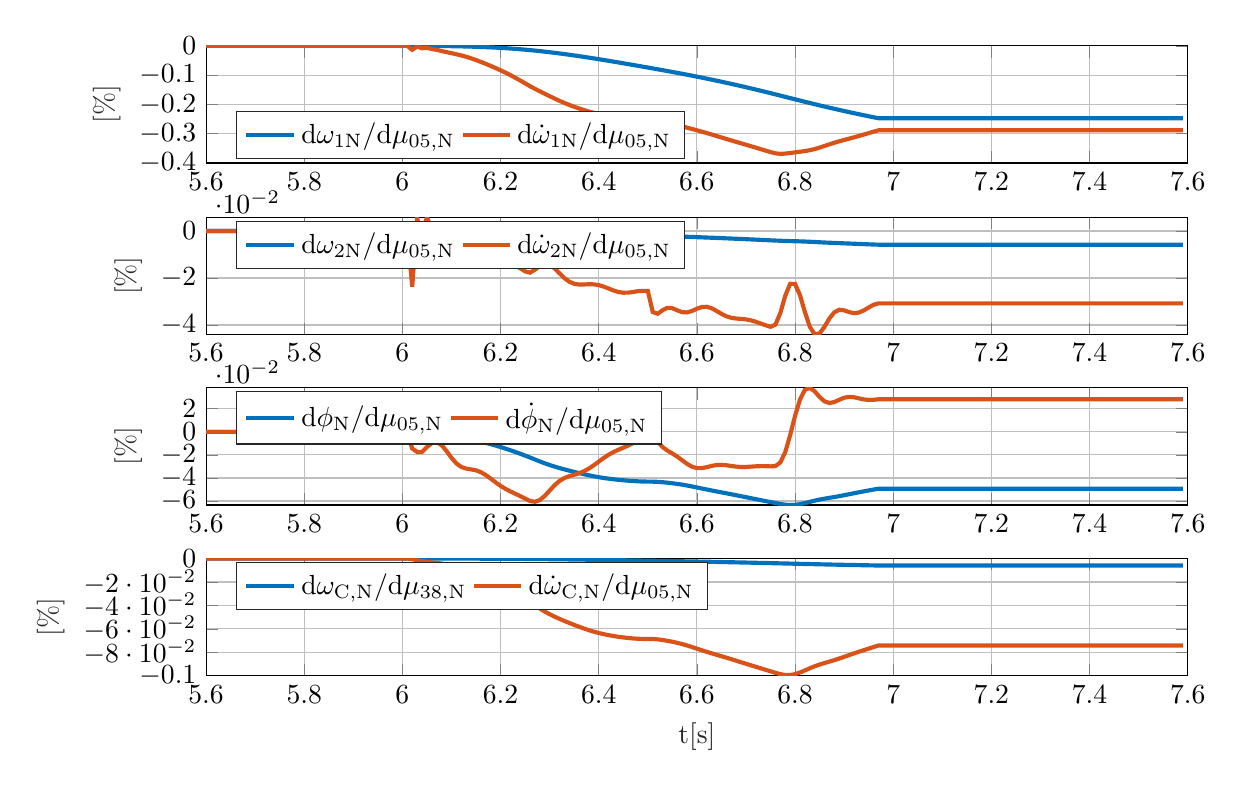
\begin{tikzpicture}

\begin{axis}[%
width=0.959\muuwidth,
height=0.186\muuheight,
at={(0\muuwidth,0.814\muuheight)},
scale only axis,
xmin=5.6,
xmax=7.6,
ymin=-0.4,
ymax=0,
ylabel style={font=\color{white!15!black}},
ylabel={[$\%$]},
axis background/.style={fill=white},
xmajorgrids,
ymajorgrids,
legend style={at={(0.03,0.03)}, anchor=south west, legend columns=2, legend cell align=left, align=left, draw=white!15!black}
]
\addplot [color=mycolor1, line width=1.5pt]
  table[row sep=crcr]{%
5.59	0\\
5.6	0\\
5.61	0\\
5.62	0\\
5.63	0\\
5.64	0\\
5.65	0\\
5.66	0\\
5.67	0\\
5.68	0\\
5.69	0\\
5.7	0\\
5.71	0\\
5.72	0\\
5.73	0\\
5.74	0\\
5.75	0\\
5.76	0\\
5.77	0\\
5.78	0\\
5.79	0\\
5.8	0\\
5.81	0\\
5.82	0\\
5.83	0\\
5.84	0\\
5.85	0\\
5.86	0\\
5.87	0\\
5.88	0\\
5.89	0\\
5.9	0\\
5.91	0\\
5.92	0\\
5.93	0\\
5.94	0\\
5.95	0\\
5.96	0\\
5.97	0\\
5.98	0\\
5.99	0\\
6	0\\
6.01	0\\
6.02	-0.000104400984332506\\
6.03	-0.000168483871591052\\
6.04	-0.000245847138555306\\
6.05	-0.000325718384631463\\
6.06	-0.000432523897041306\\
6.07	-0.000573205504899566\\
6.08	-0.000756989542202283\\
6.09	-0.000983418293194439\\
6.1	-0.0012530367472859\\
6.11	-0.00156370733283048\\
6.12	-0.00191957131870351\\
6.13	-0.00232452926885557\\
6.14	-0.0027868725910303\\
6.15	-0.00331367600780347\\
6.16	-0.0039114980280715\\
6.17	-0.00458485478701748\\
6.18	-0.00533747085376776\\
6.19	-0.00617250026364947\\
6.2	-0.00709332192251671\\
6.21	-0.00810434083192625\\
6.22	-0.00921035447681127\\
6.23	-0.010416713923873\\
6.24	-0.0117285653366722\\
6.25	-0.0131506708692321\\
6.26	-0.0146955478177824\\
6.27	-0.0163445106277059\\
6.28	-0.0180886123695395\\
6.29	-0.0199299381257615\\
6.3	-0.0218668126008731\\
6.31	-0.0238977487972777\\
6.32	-0.0260199530645098\\
6.33	-0.0282291197781273\\
6.34	-0.0305197679824981\\
6.35	-0.0328860391995766\\
6.36	-0.0353221701350696\\
6.37	-0.0378228632633518\\
6.38	-0.0403832260419867\\
6.39	-0.0429987334783707\\
6.4	-0.0456651629270352\\
6.41	-0.0483783959985065\\
6.42	-0.0511345362425451\\
6.43	-0.0539293846102797\\
6.44	-0.0567585123753063\\
6.45	-0.0596170542125833\\
6.46	-0.0624996239345174\\
6.47	-0.0654010287579518\\
6.48	-0.0683160150903335\\
6.49	-0.0712400695844238\\
6.5	-0.0741692387489206\\
6.51	-0.0771327254704923\\
6.52	-0.08013033346743\\
6.53	-0.0831440527883826\\
6.54	-0.0861767729085173\\
6.55	-0.0892393951159003\\
6.56	-0.0923416806545795\\
6.57	-0.0954909722580845\\
6.58	-0.0986907081625417\\
6.59	-0.101941836723187\\
6.6	-0.105244662138097\\
6.61	-0.108600035752658\\
6.62	-0.112009630853188\\
6.63	-0.115475508873146\\
6.64	-0.118999452013326\\
6.65	-0.122582335229309\\
6.66	-0.126224051416582\\
6.67	-0.129923798194889\\
6.68	-0.133680628992057\\
6.69	-0.137493930921379\\
6.7	-0.1413636466253\\
6.71	-0.145290224123668\\
6.72	-0.149274321807595\\
6.73	-0.153316500970963\\
6.74	-0.157417027107467\\
6.75	-0.161575857797966\\
6.76	-0.165792890811718\\
6.77	-0.170042077117942\\
6.78	-0.174296208190889\\
6.79	-0.178532097515652\\
6.8	-0.182742080157556\\
6.81	-0.186927802005202\\
6.82	-0.191088731656021\\
6.83	-0.195220012279357\\
6.84	-0.199311576205623\\
6.85	-0.203351445502325\\
6.86	-0.207330165564797\\
6.87	-0.21124369969911\\
6.88	-0.215093438132319\\
6.89	-0.218883991261696\\
6.9	-0.222620189040342\\
6.91	-0.226304858551343\\
6.92	-0.229938163634203\\
6.93	-0.233518341293205\\
6.94	-0.237043133612395\\
6.95	-0.240510974527253\\
6.96	-0.243921510072634\\
6.97	-0.247130796051239\\
6.98	-0.247130796051239\\
6.99	-0.247130796051239\\
7	-0.247130796051239\\
7.01	-0.247130796051239\\
7.02	-0.247130796051239\\
7.03	-0.247130796051239\\
7.04	-0.247130796051239\\
7.05	-0.247130796051239\\
7.06	-0.247130796051239\\
7.07	-0.247130796051239\\
7.08	-0.247130796051239\\
7.09	-0.247130796051239\\
7.1	-0.247130796051239\\
7.11	-0.247130796051239\\
7.12	-0.247130796051239\\
7.13	-0.247130796051239\\
7.14	-0.247130796051239\\
7.15	-0.247130796051239\\
7.16	-0.247130796051239\\
7.17	-0.247130796051239\\
7.18	-0.247130796051239\\
7.19	-0.247130796051239\\
7.2	-0.247130796051239\\
7.21	-0.247130796051239\\
7.22	-0.247130796051239\\
7.23	-0.247130796051239\\
7.24	-0.247130796051239\\
7.25	-0.247130796051239\\
7.26	-0.247130796051239\\
7.27	-0.247130796051239\\
7.28	-0.247130796051239\\
7.29	-0.247130796051239\\
7.3	-0.247130796051239\\
7.31	-0.247130796051239\\
7.32	-0.247130796051239\\
7.33	-0.247130796051239\\
7.34	-0.247130796051239\\
7.35	-0.247130796051239\\
7.36	-0.247130796051239\\
7.37	-0.247130796051239\\
7.38	-0.247130796051239\\
7.39	-0.247130796051239\\
7.4	-0.247130796051239\\
7.41	-0.247130796051239\\
7.42	-0.247130796051239\\
7.43	-0.247130796051239\\
7.44	-0.247130796051239\\
7.45	-0.247130796051239\\
7.46	-0.247130796051239\\
7.47	-0.247130796051239\\
7.48	-0.247130796051239\\
7.49	-0.247130796051239\\
7.5	-0.247130796051239\\
7.51	-0.247130796051239\\
7.52	-0.247130796051239\\
7.53	-0.247130796051239\\
7.54	-0.247130796051239\\
7.55	-0.247130796051239\\
7.56	-0.247130796051239\\
7.57	-0.247130796051239\\
7.58	-0.247130796051239\\
7.59	-0.247130796051239\\
};
\addlegendentry{d$\omega_{1\mathrm{N}}/$d$\mu_\mathrm{05,N}$}

\addplot [color=mycolor2, line width=1.5pt]
  table[row sep=crcr]{%
5.59	0\\
5.6	0\\
5.61	0\\
5.62	0\\
5.63	0\\
5.64	0\\
5.65	0\\
5.66	0\\
5.67	0\\
5.68	0\\
5.69	0\\
5.7	0\\
5.71	0\\
5.72	0\\
5.73	0\\
5.74	0\\
5.75	0\\
5.76	0\\
5.77	0\\
5.78	0\\
5.79	0\\
5.8	0\\
5.81	0\\
5.82	0\\
5.83	0\\
5.84	0\\
5.85	0\\
5.86	0\\
5.87	0\\
5.88	0\\
5.89	0\\
5.9	0\\
5.91	0\\
5.92	0\\
5.93	0\\
5.94	0\\
5.95	0\\
5.96	0\\
5.97	0\\
5.98	0\\
5.99	0\\
6	0\\
6.01	0\\
6.02	-0.0136760168903676\\
6.03	-0.00230641969544813\\
6.04	-0.00848032186324539\\
6.05	-0.00691046480190366\\
6.06	-0.0110763873632093\\
6.07	-0.0137541339030696\\
6.08	-0.0179079096861972\\
6.09	-0.021446010788216\\
6.1	-0.0251447801379912\\
6.11	-0.0288121501470446\\
6.12	-0.0328552127207012\\
6.13	-0.0374599930251475\\
6.14	-0.0427352012130729\\
6.15	-0.0486193712867506\\
6.16	-0.0550040339790628\\
6.17	-0.0617174452089849\\
6.18	-0.0687306436332972\\
6.19	-0.0759966983350535\\
6.2	-0.0836134410785814\\
6.21	-0.0916290456243324\\
6.22	-0.100083345883053\\
6.23	-0.109013481247706\\
6.24	-0.11835374344487\\
6.25	-0.128118551777758\\
6.26	-0.137870216902648\\
6.27	-0.146819744298646\\
6.28	-0.155338592829727\\
6.29	-0.163681662369641\\
6.3	-0.171897594878516\\
6.31	-0.179953407203097\\
6.32	-0.187690984463978\\
6.33	-0.195001039283605\\
6.34	-0.201805435275214\\
6.35	-0.20810445583942\\
6.36	-0.213917936548742\\
6.37	-0.219295437634848\\
6.38	-0.224261459574566\\
6.39	-0.228856596908929\\
6.4	-0.233083169298556\\
6.41	-0.236972146496811\\
6.42	-0.240512921889188\\
6.43	-0.243675558515224\\
6.44	-0.246447541554693\\
6.45	-0.248761015758005\\
6.46	-0.250615574685369\\
6.47	-0.252021263568385\\
6.48	-0.252978090937939\\
6.49	-0.253606963237042\\
6.5	-0.253849603307175\\
6.51	-0.258711081754536\\
6.52	-0.260447123002865\\
6.53	-0.261778349903242\\
6.54	-0.263840976048732\\
6.55	-0.266894590427945\\
6.56	-0.270720951494552\\
6.57	-0.274992574668851\\
6.58	-0.279424288582649\\
6.59	-0.283887772759629\\
6.6	-0.28839061192918\\
6.61	-0.29300514730516\\
6.62	-0.297791318784533\\
6.63	-0.302754562854995\\
6.64	-0.307837740261136\\
6.65	-0.312952356049253\\
6.66	-0.318020465180392\\
6.67	-0.323004883524984\\
6.68	-0.327916094383882\\
6.69	-0.33279747905088\\
6.7	-0.337698881865595\\
6.71	-0.342652871761729\\
6.72	-0.347663830012484\\
6.73	-0.352712379371386\\
6.74	-0.357769224903295\\
6.75	-0.362810045773301\\
6.76	-0.367039256847731\\
6.77	-0.368793468953395\\
6.78	-0.36800321617163\\
6.79	-0.365928814660984\\
6.8	-0.363682357735669\\
6.81	-0.361576363850315\\
6.82	-0.359302055248872\\
6.83	-0.35635687835171\\
6.84	-0.352391221159775\\
6.85	-0.34743862493102\\
6.86	-0.341880096741988\\
6.87	-0.336225523110158\\
6.88	-0.330873977331618\\
6.89	-0.325972616345014\\
6.9	-0.321424601209482\\
6.91	-0.317003787265945\\
6.92	-0.312495713694287\\
6.93	-0.307792267415718\\
6.94	-0.302910113319046\\
6.95	-0.297943335454756\\
6.96	-0.292995587288017\\
6.97	-0.288448510073245\\
6.98	-0.288448510073245\\
6.99	-0.288448510073245\\
7	-0.288448510073245\\
7.01	-0.288448510073245\\
7.02	-0.288448510073245\\
7.03	-0.288448510073245\\
7.04	-0.288448510073245\\
7.05	-0.288448510073245\\
7.06	-0.288448510073245\\
7.07	-0.288448510073245\\
7.08	-0.288448510073245\\
7.09	-0.288448510073245\\
7.1	-0.288448510073245\\
7.11	-0.288448510073245\\
7.12	-0.288448510073245\\
7.13	-0.288448510073245\\
7.14	-0.288448510073245\\
7.15	-0.288448510073245\\
7.16	-0.288448510073245\\
7.17	-0.288448510073245\\
7.18	-0.288448510073245\\
7.19	-0.288448510073245\\
7.2	-0.288448510073245\\
7.21	-0.288448510073245\\
7.22	-0.288448510073245\\
7.23	-0.288448510073245\\
7.24	-0.288448510073245\\
7.25	-0.288448510073245\\
7.26	-0.288448510073245\\
7.27	-0.288448510073245\\
7.28	-0.288448510073245\\
7.29	-0.288448510073245\\
7.3	-0.288448510073245\\
7.31	-0.288448510073245\\
7.32	-0.288448510073245\\
7.33	-0.288448510073245\\
7.34	-0.288448510073245\\
7.35	-0.288448510073245\\
7.36	-0.288448510073245\\
7.37	-0.288448510073245\\
7.38	-0.288448510073245\\
7.39	-0.288448510073245\\
7.4	-0.288448510073245\\
7.41	-0.288448510073245\\
7.42	-0.288448510073245\\
7.43	-0.288448510073245\\
7.44	-0.288448510073245\\
7.45	-0.288448510073245\\
7.46	-0.288448510073245\\
7.47	-0.288448510073245\\
7.48	-0.288448510073245\\
7.49	-0.288448510073245\\
7.5	-0.288448510073245\\
7.51	-0.288448510073245\\
7.52	-0.288448510073245\\
7.53	-0.288448510073245\\
7.54	-0.288448510073245\\
7.55	-0.288448510073245\\
7.56	-0.288448510073245\\
7.57	-0.288448510073245\\
7.58	-0.288448510073245\\
7.59	-0.288448510073245\\
};
\addlegendentry{d$\dot{\omega}_{1\mathrm{N}}/$d$\mu_\mathrm{05,N}$}

\end{axis}

\begin{axis}[%
width=0.959\muuwidth,
height=0.186\muuheight,
at={(0\muuwidth,0.542\muuheight)},
scale only axis,
xmin=5.6,
xmax=7.6,
ymin=-0.0439559974941892,
ymax=0.00587492890815738,
ylabel style={font=\color{white!15!black}},
ylabel={[$\%$]},
axis background/.style={fill=white},
xmajorgrids,
ymajorgrids,
legend style={at={(0.03,0.97)}, anchor=north west, legend columns=2, legend cell align=left, align=left, draw=white!15!black}
]
\addplot [color=mycolor1, line width=1.5pt]
  table[row sep=crcr]{%
5.59	0\\
5.6	0\\
5.61	0\\
5.62	0\\
5.63	0\\
5.64	0\\
5.65	0\\
5.66	0\\
5.67	0\\
5.68	0\\
5.69	0\\
5.7	0\\
5.71	0\\
5.72	0\\
5.73	0\\
5.74	0\\
5.75	0\\
5.76	0\\
5.77	0\\
5.78	0\\
5.79	0\\
5.8	0\\
5.81	0\\
5.82	0\\
5.83	0\\
5.84	0\\
5.85	0\\
5.86	0\\
5.87	0\\
5.88	0\\
5.89	0\\
5.9	0\\
5.91	0\\
5.92	0\\
5.93	0\\
5.94	0\\
5.95	0\\
5.96	0\\
5.97	0\\
5.98	0\\
5.99	0\\
6	0\\
6.01	0\\
6.02	-4.2013454439802e-05\\
6.03	-5.15927813846213e-05\\
6.04	-5.36037584563943e-05\\
6.05	-4.39289160262182e-05\\
6.06	-3.73321586537379e-05\\
6.07	-3.82464048149639e-05\\
6.08	-5.01620468939701e-05\\
6.09	-6.95774494452468e-05\\
6.1	-9.22608148999139e-05\\
6.11	-0.000112907981479714\\
6.12	-0.000130162948078499\\
6.13	-0.000143957704549452\\
6.14	-0.000157155411183878\\
6.15	-0.000172291721749755\\
6.16	-0.000191294668781523\\
6.17	-0.000214563520825576\\
6.18	-0.000241461748584628\\
6.19	-0.000270805176729097\\
6.2	-0.000301545056084727\\
6.21	-0.000333367598378396\\
6.22	-0.00036646349677488\\
6.23	-0.000401501238733338\\
6.24	-0.000439129881896243\\
6.25	-0.000479775261081166\\
6.26	-0.00052322332688976\\
6.27	-0.000565386291180277\\
6.28	-0.000603822253841713\\
6.29	-0.00063910649508388\\
6.3	-0.000673738707395795\\
6.31	-0.000710825769411098\\
6.32	-0.000752516835107717\\
6.33	-0.000799420948504204\\
6.34	-0.00085078253760013\\
6.35	-0.000905138244391082\\
6.36	-0.00096092418062223\\
6.37	-0.00101701712978362\\
6.38	-0.00107290349169558\\
6.39	-0.00112867538344484\\
6.4	-0.00118490044145712\\
6.41	-0.00124228452099303\\
6.42	-0.00130149744572589\\
6.43	-0.00136277631288799\\
6.44	-0.00142591620601253\\
6.45	-0.00149027092032244\\
6.46	-0.00155491807929043\\
6.47	-0.0016191751269402\\
6.48	-0.00168261739111607\\
6.49	-0.00174543455235024\\
6.5	-0.00180819822532551\\
6.51	-0.00188461474987791\\
6.52	-0.00197124592492412\\
6.53	-0.00205617505869647\\
6.54	-0.00213767986162129\\
6.55	-0.00221816472686497\\
6.56	-0.00230009276384976\\
6.57	-0.0023842388776201\\
6.58	-0.00246955720230535\\
6.59	-0.00255419387780402\\
6.6	-0.00263678482357245\\
6.61	-0.00271721926147896\\
6.62	-0.002796597762691\\
6.63	-0.00287662525170325\\
6.64	-0.00295887264323023\\
6.65	-0.0030441096446738\\
6.66	-0.00313220812253541\\
6.67	-0.00322239397071898\\
6.68	-0.00331374949222153\\
6.69	-0.0034056496087541\\
6.7	-0.00349796446085064\\
6.71	-0.0035910154782975\\
6.72	-0.00368531317280511\\
6.73	-0.00378128550614555\\
6.74	-0.00387910443957415\\
6.75	-0.00397867621714177\\
6.76	-0.00407845775498897\\
6.77	-0.00417107548730192\\
6.78	-0.0042478688799335\\
6.79	-0.00430837220406552\\
6.8	-0.00436269847805635\\
6.81	-0.00442337437518194\\
6.82	-0.00449925458125941\\
6.83	-0.00459225912487605\\
6.84	-0.00469727554874632\\
6.85	-0.00480569455102098\\
6.86	-0.00490977557924267\\
6.87	-0.00500563542249163\\
6.88	-0.00509370663703862\\
6.89	-0.0051772175198666\\
6.9	-0.00525984141482926\\
6.91	-0.00534384900907602\\
6.92	-0.00542946603167724\\
6.93	-0.00551536820579175\\
6.94	-0.00559978379640225\\
6.95	-0.00568145465454762\\
6.96	-0.00576009191795606\\
6.97	-0.00583297151159157\\
6.98	-0.00583297151159157\\
6.99	-0.00583297151159157\\
7	-0.00583297151159157\\
7.01	-0.00583297151159157\\
7.02	-0.00583297151159157\\
7.03	-0.00583297151159157\\
7.04	-0.00583297151159157\\
7.05	-0.00583297151159157\\
7.06	-0.00583297151159157\\
7.07	-0.00583297151159157\\
7.08	-0.00583297151159157\\
7.09	-0.00583297151159157\\
7.1	-0.00583297151159157\\
7.11	-0.00583297151159157\\
7.12	-0.00583297151159157\\
7.13	-0.00583297151159157\\
7.14	-0.00583297151159157\\
7.15	-0.00583297151159157\\
7.16	-0.00583297151159157\\
7.17	-0.00583297151159157\\
7.18	-0.00583297151159157\\
7.19	-0.00583297151159157\\
7.2	-0.00583297151159157\\
7.21	-0.00583297151159157\\
7.22	-0.00583297151159157\\
7.23	-0.00583297151159157\\
7.24	-0.00583297151159157\\
7.25	-0.00583297151159157\\
7.26	-0.00583297151159157\\
7.27	-0.00583297151159157\\
7.28	-0.00583297151159157\\
7.29	-0.00583297151159157\\
7.3	-0.00583297151159157\\
7.31	-0.00583297151159157\\
7.32	-0.00583297151159157\\
7.33	-0.00583297151159157\\
7.34	-0.00583297151159157\\
7.35	-0.00583297151159157\\
7.36	-0.00583297151159157\\
7.37	-0.00583297151159157\\
7.38	-0.00583297151159157\\
7.39	-0.00583297151159157\\
7.4	-0.00583297151159157\\
7.41	-0.00583297151159157\\
7.42	-0.00583297151159157\\
7.43	-0.00583297151159157\\
7.44	-0.00583297151159157\\
7.45	-0.00583297151159157\\
7.46	-0.00583297151159157\\
7.47	-0.00583297151159157\\
7.48	-0.00583297151159157\\
7.49	-0.00583297151159157\\
7.5	-0.00583297151159157\\
7.51	-0.00583297151159157\\
7.52	-0.00583297151159157\\
7.53	-0.00583297151159157\\
7.54	-0.00583297151159157\\
7.55	-0.00583297151159157\\
7.56	-0.00583297151159157\\
7.57	-0.00583297151159157\\
7.58	-0.00583297151159157\\
7.59	-0.00583297151159157\\
};
\addlegendentry{d$\omega_{2\mathrm{N}}/$d$\mu_\mathrm{05,N}$}

\addplot [color=mycolor2, line width=1.5pt]
  table[row sep=crcr]{%
5.59	0\\
5.6	0\\
5.61	0\\
5.62	0\\
5.63	0\\
5.64	0\\
5.65	0\\
5.66	0\\
5.67	0\\
5.68	0\\
5.69	0\\
5.7	0\\
5.71	0\\
5.72	0\\
5.73	0\\
5.74	0\\
5.75	0\\
5.76	0\\
5.77	0\\
5.78	0\\
5.79	0\\
5.8	0\\
5.81	0\\
5.82	0\\
5.83	0\\
5.84	0\\
5.85	0\\
5.86	0\\
5.87	0\\
5.88	0\\
5.89	0\\
5.9	0\\
5.91	0\\
5.92	0\\
5.93	0\\
5.94	0\\
5.95	0\\
5.96	0\\
5.97	0\\
5.98	0\\
5.99	0\\
6	0\\
6.01	0\\
6.02	-0.023662008948169\\
6.03	0.0054272090852318\\
6.04	-0.00162778323619019\\
6.05	0.00587492890815738\\
6.06	0.000480861453933386\\
6.07	-0.00214173500063908\\
6.08	-0.00692599625526033\\
6.09	-0.00878991589476526\\
6.1	-0.00907566943528146\\
6.11	-0.00774466188487237\\
6.12	-0.00617233698514052\\
6.13	-0.00529498383579826\\
6.14	-0.0055738236295264\\
6.15	-0.00683717925997916\\
6.16	-0.00860760021359188\\
6.17	-0.0102560848605596\\
6.18	-0.0115167919677272\\
6.19	-0.0122398097373913\\
6.2	-0.0127071020705859\\
6.21	-0.0131521571496875\\
6.22	-0.0137814317729214\\
6.23	-0.0147317831073623\\
6.24	-0.015867382856156\\
6.25	-0.0171775358968982\\
6.26	-0.0177293432582226\\
6.27	-0.0164615674956647\\
6.28	-0.0148155670737541\\
6.29	-0.0139735745108623\\
6.3	-0.0143649217873037\\
6.31	-0.0159110041170394\\
6.32	-0.0180031300781103\\
6.33	-0.0200455163503051\\
6.34	-0.0215805680132714\\
6.35	-0.0224681025485781\\
6.36	-0.0227762826710906\\
6.37	-0.0227549262399483\\
6.38	-0.0226467332742804\\
6.39	-0.0227034874663343\\
6.4	-0.0230197832207734\\
6.41	-0.0236501987041333\\
6.42	-0.0244764823144203\\
6.43	-0.0252974789003357\\
6.44	-0.0259589050743611\\
6.45	-0.0262561637919004\\
6.46	-0.0262153842536693\\
6.47	-0.0259516491006967\\
6.48	-0.0255944348898489\\
6.49	-0.0254847597619296\\
6.5	-0.0255201136256952\\
6.51	-0.0344409723113637\\
6.52	-0.0352248912651131\\
6.53	-0.0337157636575268\\
6.54	-0.0326831098297488\\
6.55	-0.0328602491007546\\
6.56	-0.0337485837790465\\
6.57	-0.0345377806419574\\
6.58	-0.0346409974871563\\
6.59	-0.034017705827634\\
6.6	-0.0330700425616154\\
6.61	-0.0323494455014849\\
6.62	-0.0322534230364112\\
6.63	-0.0328760967687945\\
6.64	-0.0339975023869745\\
6.65	-0.0352425906581631\\
6.66	-0.0362742248033697\\
6.67	-0.0369282101629299\\
6.68	-0.0372447068122319\\
6.69	-0.0374044317446263\\
6.7	-0.0376160007254437\\
6.71	-0.0380158935917799\\
6.72	-0.0386234628976752\\
6.73	-0.039360002333445\\
6.74	-0.0401068737648029\\
6.75	-0.0407659464188631\\
6.76	-0.0398404560645771\\
6.77	-0.0348666674373978\\
6.78	-0.0275519819511783\\
6.79	-0.0224816087429864\\
6.8	-0.0225447438573311\\
6.81	-0.0273190140039992\\
6.82	-0.0344398472207441\\
6.83	-0.0407445625053669\\
6.84	-0.0439559974941892\\
6.85	-0.0435764800135993\\
6.86	-0.0407167131729686\\
6.87	-0.0372020893839443\\
6.88	-0.0345836959442584\\
6.89	-0.0335234263661021\\
6.9	-0.0337589315774724\\
6.91	-0.03450040304421\\
6.92	-0.0349560704371442\\
6.93	-0.0347042521048449\\
6.94	-0.0337859636054267\\
6.95	-0.0325448351498589\\
6.96	-0.0313787181511334\\
6.97	-0.0307879577426244\\
6.98	-0.0307879577426244\\
6.99	-0.0307879577426244\\
7	-0.0307879577426244\\
7.01	-0.0307879577426244\\
7.02	-0.0307879577426244\\
7.03	-0.0307879577426244\\
7.04	-0.0307879577426244\\
7.05	-0.0307879577426244\\
7.06	-0.0307879577426244\\
7.07	-0.0307879577426244\\
7.08	-0.0307879577426244\\
7.09	-0.0307879577426244\\
7.1	-0.0307879577426244\\
7.11	-0.0307879577426244\\
7.12	-0.0307879577426244\\
7.13	-0.0307879577426244\\
7.14	-0.0307879577426244\\
7.15	-0.0307879577426244\\
7.16	-0.0307879577426244\\
7.17	-0.0307879577426244\\
7.18	-0.0307879577426244\\
7.19	-0.0307879577426244\\
7.2	-0.0307879577426244\\
7.21	-0.0307879577426244\\
7.22	-0.0307879577426244\\
7.23	-0.0307879577426244\\
7.24	-0.0307879577426244\\
7.25	-0.0307879577426244\\
7.26	-0.0307879577426244\\
7.27	-0.0307879577426244\\
7.28	-0.0307879577426244\\
7.29	-0.0307879577426244\\
7.3	-0.0307879577426244\\
7.31	-0.0307879577426244\\
7.32	-0.0307879577426244\\
7.33	-0.0307879577426244\\
7.34	-0.0307879577426244\\
7.35	-0.0307879577426244\\
7.36	-0.0307879577426244\\
7.37	-0.0307879577426244\\
7.38	-0.0307879577426244\\
7.39	-0.0307879577426244\\
7.4	-0.0307879577426244\\
7.41	-0.0307879577426244\\
7.42	-0.0307879577426244\\
7.43	-0.0307879577426244\\
7.44	-0.0307879577426244\\
7.45	-0.0307879577426244\\
7.46	-0.0307879577426244\\
7.47	-0.0307879577426244\\
7.48	-0.0307879577426244\\
7.49	-0.0307879577426244\\
7.5	-0.0307879577426244\\
7.51	-0.0307879577426244\\
7.52	-0.0307879577426244\\
7.53	-0.0307879577426244\\
7.54	-0.0307879577426244\\
7.55	-0.0307879577426244\\
7.56	-0.0307879577426244\\
7.57	-0.0307879577426244\\
7.58	-0.0307879577426244\\
7.59	-0.0307879577426244\\
};
\addlegendentry{d$\dot{\omega}_{2\mathrm{N}}/$d$\mu_\mathrm{05,N}$}

\end{axis}

\begin{axis}[%
width=0.959\muuwidth,
height=0.186\muuheight,
at={(0\muuwidth,0.271\muuheight)},
scale only axis,
xmin=5.6,
xmax=7.6,
ymin=-0.0634580426004168,
ymax=0.0381187609560699,
ylabel style={font=\color{white!15!black}},
ylabel={[$\%$]},
axis background/.style={fill=white},
xmajorgrids,
ymajorgrids,
legend style={at={(0.03,0.97)}, anchor=north west, legend columns=2, legend cell align=left, align=left, draw=white!15!black}
]
\addplot [color=mycolor1, line width=1.5pt]
  table[row sep=crcr]{%
5.59	0\\
5.6	0\\
5.61	0\\
5.62	0\\
5.63	0\\
5.64	0\\
5.65	0\\
5.66	0\\
5.67	0\\
5.68	0\\
5.69	0\\
5.7	0\\
5.71	0\\
5.72	0\\
5.73	0\\
5.74	0\\
5.75	0\\
5.76	0\\
5.77	0\\
5.78	0\\
5.79	0\\
5.8	0\\
5.81	0\\
5.82	0\\
5.83	0\\
5.84	0\\
5.85	0\\
5.86	0\\
5.87	0\\
5.88	0\\
5.89	0\\
5.9	0\\
5.91	0\\
5.92	0\\
5.93	0\\
5.94	0\\
5.95	0\\
5.96	0\\
5.97	0\\
5.98	0\\
5.99	0\\
6	0\\
6.01	0\\
6.02	-0.000134902172146005\\
6.03	-0.000650904354894073\\
6.04	-0.00112670628211098\\
6.05	-0.00157465231572442\\
6.06	-0.00188735817055099\\
6.07	-0.00214610359025403\\
6.08	-0.00242491707476553\\
6.09	-0.00282038991670973\\
6.1	-0.003373844013547\\
6.11	-0.00408152611357056\\
6.12	-0.00490126239545573\\
6.13	-0.00578374731889271\\
6.14	-0.00669355911407994\\
6.15	-0.00762276218877757\\
6.16	-0.00858534016132743\\
6.17	-0.00960511252910141\\
6.18	-0.0107043515750607\\
6.19	-0.0118945430579214\\
6.2	-0.013173920892597\\
6.21	-0.0145324752628951\\
6.22	-0.0159585500360618\\
6.23	-0.0174438060450819\\
6.24	-0.0189858716346963\\
6.25	-0.0205866719021213\\
6.26	-0.0222536842542335\\
6.27	-0.0239590488545301\\
6.28	-0.0256522901446773\\
6.29	-0.0272709333963129\\
6.3	-0.028772252684985\\
6.31	-0.030141061796889\\
6.32	-0.0313918136102778\\
6.33	-0.0325543333703537\\
6.34	-0.0336586227497976\\
6.35	-0.0347240480654324\\
6.36	-0.0357554394780666\\
6.37	-0.0367445356363714\\
6.38	-0.0376761193117657\\
6.39	-0.0385339555377044\\
6.4	-0.0393065447114909\\
6.41	-0.0399903804037691\\
6.42	-0.0405901331082206\\
6.43	-0.0411166046692024\\
6.44	-0.0415817979653187\\
6.45	-0.0419945238144524\\
6.46	-0.0423564667036375\\
6.47	-0.0426620372130894\\
6.48	-0.0429012238547334\\
6.49	-0.0430637160774328\\
6.5	-0.0431447534787606\\
6.51	-0.0431940004642103\\
6.52	-0.0433601421273885\\
6.53	-0.0436687357795544\\
6.54	-0.0440856123043029\\
6.55	-0.0445808157140697\\
6.56	-0.0451482114574862\\
6.57	-0.0457983182626347\\
6.58	-0.0465382419224843\\
6.59	-0.0473583394857213\\
6.6	-0.0482312234993656\\
6.61	-0.049121371417641\\
6.62	-0.0499985925015419\\
6.63	-0.050846899843072\\
6.64	-0.0516677571139179\\
6.65	-0.0524748704170829\\
6.66	-0.0532849790628635\\
6.67	-0.0541099610414732\\
6.68	-0.0549527385558386\\
6.69	-0.0558081226161237\\
6.7	-0.0566671012202182\\
6.71	-0.0575217269621665\\
6.72	-0.0583684937305136\\
6.73	-0.0592087973183934\\
6.74	-0.0600471050683161\\
6.75	-0.0608882835538374\\
6.76	-0.0617312655401892\\
6.77	-0.0625327897945416\\
6.78	-0.0631695900950518\\
6.79	-0.0634580426004168\\
6.8	-0.0632863740676485\\
6.81	-0.0626835383965387\\
6.82	-0.0617590855774767\\
6.83	-0.0606943801324416\\
6.84	-0.0596549912774439\\
6.85	-0.0587343365850601\\
6.86	-0.0579405050492916\\
6.87	-0.0572216751232724\\
6.88	-0.0565089824192733\\
6.89	-0.0557536541721519\\
6.9	-0.054943339995559\\
6.91	-0.0540965616680717\\
6.92	-0.0532443563288501\\
6.93	-0.0524115929734793\\
6.94	-0.0516064912659769\\
6.95	-0.0508215869229832\\
6.96	-0.0500414316856867\\
6.97	-0.0492866606581692\\
6.98	-0.0492866606581692\\
6.99	-0.0492866606581692\\
7	-0.0492866606581692\\
7.01	-0.0492866606581692\\
7.02	-0.0492866606581692\\
7.03	-0.0492866606581692\\
7.04	-0.0492866606581692\\
7.05	-0.0492866606581692\\
7.06	-0.0492866606581692\\
7.07	-0.0492866606581692\\
7.08	-0.0492866606581692\\
7.09	-0.0492866606581692\\
7.1	-0.0492866606581692\\
7.11	-0.0492866606581692\\
7.12	-0.0492866606581692\\
7.13	-0.0492866606581692\\
7.14	-0.0492866606581692\\
7.15	-0.0492866606581692\\
7.16	-0.0492866606581692\\
7.17	-0.0492866606581692\\
7.18	-0.0492866606581692\\
7.19	-0.0492866606581692\\
7.2	-0.0492866606581692\\
7.21	-0.0492866606581692\\
7.22	-0.0492866606581692\\
7.23	-0.0492866606581692\\
7.24	-0.0492866606581692\\
7.25	-0.0492866606581692\\
7.26	-0.0492866606581692\\
7.27	-0.0492866606581692\\
7.28	-0.0492866606581692\\
7.29	-0.0492866606581692\\
7.3	-0.0492866606581692\\
7.31	-0.0492866606581692\\
7.32	-0.0492866606581692\\
7.33	-0.0492866606581692\\
7.34	-0.0492866606581692\\
7.35	-0.0492866606581692\\
7.36	-0.0492866606581692\\
7.37	-0.0492866606581692\\
7.38	-0.0492866606581692\\
7.39	-0.0492866606581692\\
7.4	-0.0492866606581692\\
7.41	-0.0492866606581692\\
7.42	-0.0492866606581692\\
7.43	-0.0492866606581692\\
7.44	-0.0492866606581692\\
7.45	-0.0492866606581692\\
7.46	-0.0492866606581692\\
7.47	-0.0492866606581692\\
7.48	-0.0492866606581692\\
7.49	-0.0492866606581692\\
7.5	-0.0492866606581692\\
7.51	-0.0492866606581692\\
7.52	-0.0492866606581692\\
7.53	-0.0492866606581692\\
7.54	-0.0492866606581692\\
7.55	-0.0492866606581692\\
7.56	-0.0492866606581692\\
7.57	-0.0492866606581692\\
7.58	-0.0492866606581692\\
7.59	-0.0492866606581692\\
};
\addlegendentry{d$\phi_\mathrm{N}/$d$\mu_\mathrm{05,N}$}

\addplot [color=mycolor2, line width=1.5pt]
  table[row sep=crcr]{%
5.59	0\\
5.6	0\\
5.61	0\\
5.62	0\\
5.63	0\\
5.64	0\\
5.65	0\\
5.66	0\\
5.67	0\\
5.68	0\\
5.69	0\\
5.7	0\\
5.71	0\\
5.72	0\\
5.73	0\\
5.74	0\\
5.75	0\\
5.76	0\\
5.77	0\\
5.78	0\\
5.79	0\\
5.8	0\\
5.81	0\\
5.82	0\\
5.83	0\\
5.84	0\\
5.85	0\\
5.86	0\\
5.87	0\\
5.88	0\\
5.89	0\\
5.9	0\\
5.91	0\\
5.92	0\\
5.93	0\\
5.94	0\\
5.95	0\\
5.96	0\\
5.97	0\\
5.98	0\\
5.99	0\\
6	0\\
6.01	0\\
6.02	-0.0144859481102383\\
6.03	-0.017424527862376\\
6.04	-0.017463696082453\\
6.05	-0.0131889253011026\\
6.06	-0.00980185414285984\\
6.07	-0.00886793639769293\\
6.08	-0.0115857654299159\\
6.09	-0.0166735731320655\\
6.1	-0.0225724208613165\\
6.11	-0.0273538749092969\\
6.12	-0.0304828358045688\\
6.13	-0.0318994831002074\\
6.14	-0.0325808446071724\\
6.15	-0.033394693894141\\
6.16	-0.0349902992567561\\
6.17	-0.0374739474777987\\
6.18	-0.0405787200562438\\
6.19	-0.0438417592390382\\
6.2	-0.0468479604960039\\
6.21	-0.0494429152783495\\
6.22	-0.051653988854535\\
6.23	-0.0536790546658638\\
6.24	-0.0557107347778622\\
6.25	-0.0578631714010819\\
6.26	-0.0599463466649754\\
6.27	-0.0606276380859464\\
6.28	-0.0590916720689728\\
6.29	-0.05553241473074\\
6.3	-0.050883910957119\\
6.31	-0.046301485406452\\
6.32	-0.0426004623563705\\
6.33	-0.0400441335318686\\
6.34	-0.0384051913462986\\
6.35	-0.0371997638234704\\
6.36	-0.0359061763876101\\
6.37	-0.0341603697143953\\
6.38	-0.0318184932608958\\
6.39	-0.0289558041295443\\
6.4	-0.0258194280128299\\
6.41	-0.0227062644851755\\
6.42	-0.0198979250895814\\
6.43	-0.0175197841625317\\
6.44	-0.0155369154457279\\
6.45	-0.0137562368739255\\
6.46	-0.0118879205039646\\
6.47	-0.00972844138511737\\
6.48	-0.00716950805198094\\
6.49	-0.00432173131967553\\
6.5	-0.00143088998498384\\
6.51	-0.00326690421683364\\
6.52	-0.00856864524565388\\
6.53	-0.0131224600440946\\
6.54	-0.0162698767843786\\
6.55	-0.0187957511470171\\
6.56	-0.0215162915122638\\
6.57	-0.024650165242154\\
6.58	-0.0277824949962081\\
6.59	-0.0302242208824893\\
6.6	-0.0314720344773003\\
6.61	-0.0314780075867412\\
6.62	-0.030631677810681\\
6.63	-0.0295410245732504\\
6.64	-0.028767317694094\\
6.65	-0.0285857567826298\\
6.66	-0.0289506660208479\\
6.67	-0.0295854131892065\\
6.68	-0.030161941689783\\
6.69	-0.0304566563226224\\
6.7	-0.0304228224254753\\
6.71	-0.03017488037326\\
6.72	-0.0298948083222843\\
6.73	-0.0297351391782805\\
6.74	-0.0297570555757789\\
6.75	-0.0299269333251652\\
6.76	-0.0296813593591756\\
6.77	-0.0265444737946445\\
6.78	-0.0175838259374495\\
6.79	-0.00283921137707333\\
6.8	0.0139060909906727\\
6.81	0.0280676584817816\\
6.82	0.0363881006185721\\
6.83	0.0381187609560699\\
6.84	0.0350468262979256\\
6.85	0.0302264713779693\\
6.86	0.0264155576973956\\
6.87	0.0250041921621357\\
6.88	0.0258464740727097\\
6.89	0.0277988349159234\\
6.9	0.0295562646710098\\
6.91	0.0303108222990198\\
6.92	0.0299815493323422\\
6.93	0.0290393316300455\\
6.94	0.0281149039352795\\
6.95	0.0276566174985365\\
6.96	0.0277677849229525\\
6.97	0.0282295492728481\\
6.98	0.0282295492728481\\
6.99	0.0282295492728481\\
7	0.0282295492728481\\
7.01	0.0282295492728481\\
7.02	0.0282295492728481\\
7.03	0.0282295492728481\\
7.04	0.0282295492728481\\
7.05	0.0282295492728481\\
7.06	0.0282295492728481\\
7.07	0.0282295492728481\\
7.08	0.0282295492728481\\
7.09	0.0282295492728481\\
7.1	0.0282295492728481\\
7.11	0.0282295492728481\\
7.12	0.0282295492728481\\
7.13	0.0282295492728481\\
7.14	0.0282295492728481\\
7.15	0.0282295492728481\\
7.16	0.0282295492728481\\
7.17	0.0282295492728481\\
7.18	0.0282295492728481\\
7.19	0.0282295492728481\\
7.2	0.0282295492728481\\
7.21	0.0282295492728481\\
7.22	0.0282295492728481\\
7.23	0.0282295492728481\\
7.24	0.0282295492728481\\
7.25	0.0282295492728481\\
7.26	0.0282295492728481\\
7.27	0.0282295492728481\\
7.28	0.0282295492728481\\
7.29	0.0282295492728481\\
7.3	0.0282295492728481\\
7.31	0.0282295492728481\\
7.32	0.0282295492728481\\
7.33	0.0282295492728481\\
7.34	0.0282295492728481\\
7.35	0.0282295492728481\\
7.36	0.0282295492728481\\
7.37	0.0282295492728481\\
7.38	0.0282295492728481\\
7.39	0.0282295492728481\\
7.4	0.0282295492728481\\
7.41	0.0282295492728481\\
7.42	0.0282295492728481\\
7.43	0.0282295492728481\\
7.44	0.0282295492728481\\
7.45	0.0282295492728481\\
7.46	0.0282295492728481\\
7.47	0.0282295492728481\\
7.48	0.0282295492728481\\
7.49	0.0282295492728481\\
7.5	0.0282295492728481\\
7.51	0.0282295492728481\\
7.52	0.0282295492728481\\
7.53	0.0282295492728481\\
7.54	0.0282295492728481\\
7.55	0.0282295492728481\\
7.56	0.0282295492728481\\
7.57	0.0282295492728481\\
7.58	0.0282295492728481\\
7.59	0.0282295492728481\\
};
\addlegendentry{d$\dot{\phi}_\mathrm{N}/$d$\mu_\mathrm{05,N}$}

\end{axis}

\begin{axis}[%
width=0.959\muuwidth,
height=0.186\muuheight,
at={(0\muuwidth,0\muuheight)},
scale only axis,
xmin=5.6,
xmax=7.6,
xlabel style={font=\color{white!15!black}},
xlabel={t[s]},
ymin=-0.1,
ymax=0,
ylabel style={font=\color{white!15!black}},
ylabel={[$\%$]},
axis background/.style={fill=white},
xmajorgrids,
ymajorgrids,
legend style={at={(0.03,0.97)}, anchor=north west, legend columns=2, legend cell align=left, align=left, draw=white!15!black}
]
\addplot [color=mycolor1, line width=1.5pt]
  table[row sep=crcr]{%
5.59	0\\
5.6	0\\
5.61	0\\
5.62	0\\
5.63	0\\
5.64	0\\
5.65	0\\
5.66	0\\
5.67	0\\
5.68	0\\
5.69	0\\
5.7	0\\
5.71	0\\
5.72	0\\
5.73	0\\
5.74	0\\
5.75	0\\
5.76	0\\
5.77	0\\
5.78	0\\
5.79	0\\
5.8	0\\
5.81	0\\
5.82	0\\
5.83	0\\
5.84	0\\
5.85	0\\
5.86	0\\
5.87	0\\
5.88	0\\
5.89	0\\
5.9	0\\
5.91	0\\
5.92	0\\
5.93	0\\
5.94	0\\
5.95	0\\
5.96	0\\
5.97	0\\
5.98	0\\
5.99	0\\
6	0\\
6.01	0\\
6.02	-1.65118780156998e-07\\
6.03	-1.25521162559273e-06\\
6.04	-3.15304427723432e-06\\
6.05	-5.82756374513548e-06\\
6.06	-9.01570238274659e-06\\
6.07	-1.26279516914405e-05\\
6.08	-1.66920976625553e-05\\
6.09	-2.14093950800562e-05\\
6.1	-2.7051652594728e-05\\
6.11	-3.38857458829978e-05\\
6.12	-4.21015191350204e-05\\
6.13	-5.18037774611681e-05\\
6.14	-6.30331537216421e-05\\
6.15	-7.58183978833497e-05\\
6.16	-9.02118768699037e-05\\
6.17	-0.000106305808619574\\
6.18	-0.000124234763088507\\
6.19	-0.000144151711575373\\
6.2	-0.000166207097630166\\
6.21	-0.000190533203147263\\
6.22	-0.000217241666482332\\
6.23	-0.000246429340562023\\
6.24	-0.000278188819133907\\
6.25	-0.000312616192943734\\
6.26	-0.000350046355126655\\
6.27	-0.000390241318631809\\
6.28	-0.000433114709043341\\
6.29	-0.000478681459517005\\
6.3	-0.0005267429070794\\
6.31	-0.000577068321445819\\
6.32	-0.000629451472087521\\
6.33	-0.000683740781058441\\
6.34	-0.000739837342942114\\
6.35	-0.000797675653220011\\
6.36	-0.000857198884780372\\
6.37	-0.000918335548788049\\
6.38	-0.000980987613283799\\
6.39	-0.00104502978518009\\
6.4	-0.00111031578087962\\
6.41	-0.00117669374423731\\
6.42	-0.00124401995302471\\
6.43	-0.00131216931103536\\
6.44	-0.00138103779952636\\
6.45	-0.00145053700652333\\
6.46	-0.00152058183668737\\
6.47	-0.00159107769518373\\
6.48	-0.00166191275168992\\
6.49	-0.00173295714349392\\
6.5	-0.00180407245632599\\
6.51	-0.00187518524654473\\
6.52	-0.00194650057849949\\
6.53	-0.00201827454913023\\
6.54	-0.00209068712350206\\
6.55	-0.00216387533226079\\
6.56	-0.00223794434761183\\
6.57	-0.00231303736888389\\
6.58	-0.0023893070666139\\
6.59	-0.00246689020075652\\
6.6	-0.00254587669472948\\
6.61	-0.00262629422988787\\
6.62	-0.00270811804532117\\
6.63	-0.002791296678539\\
6.64	-0.0028757795962672\\
6.65	-0.00296154148390773\\
6.66	-0.00304858616047389\\
6.67	-0.00313693868052394\\
6.68	-0.00322662906719495\\
6.69	-0.00331767818462416\\
6.7	-0.00341009118474962\\
6.71	-0.0035038588914593\\
6.72	-0.00359896610119747\\
6.73	-0.00369540012462336\\
6.74	-0.00379315617296147\\
6.75	-0.0038922376269224\\
6.76	-0.0039927290423951\\
6.77	-0.00409440934385417\\
6.78	-0.00419708952902105\\
6.79	-0.00430018890137788\\
6.8	-0.00440289099240599\\
6.81	-0.0045044785712375\\
6.82	-0.00460439607268446\\
6.83	-0.00470240073682076\\
6.84	-0.00479854309584448\\
6.85	-0.00489303702912047\\
6.86	-0.00498610914860001\\
6.87	-0.00507789211235586\\
6.88	-0.00516839698537629\\
6.89	-0.00525754841863887\\
6.9	-0.00534524972285446\\
6.91	-0.00543143753067029\\
6.92	-0.00551610369086959\\
6.93	-0.00559928426505579\\
6.94	-0.00568102964284598\\
6.95	-0.00576137691368279\\
6.96	-0.00584033567426622\\
6.97	-0.00591454958082878\\
6.98	-0.00591454958082878\\
6.99	-0.00591454958082878\\
7	-0.00591454958082878\\
7.01	-0.00591454958082878\\
7.02	-0.00591454958082878\\
7.03	-0.00591454958082878\\
7.04	-0.00591454958082878\\
7.05	-0.00591454958082878\\
7.06	-0.00591454958082878\\
7.07	-0.00591454958082878\\
7.08	-0.00591454958082878\\
7.09	-0.00591454958082878\\
7.1	-0.00591454958082878\\
7.11	-0.00591454958082878\\
7.12	-0.00591454958082878\\
7.13	-0.00591454958082878\\
7.14	-0.00591454958082878\\
7.15	-0.00591454958082878\\
7.16	-0.00591454958082878\\
7.17	-0.00591454958082878\\
7.18	-0.00591454958082878\\
7.19	-0.00591454958082878\\
7.2	-0.00591454958082878\\
7.21	-0.00591454958082878\\
7.22	-0.00591454958082878\\
7.23	-0.00591454958082878\\
7.24	-0.00591454958082878\\
7.25	-0.00591454958082878\\
7.26	-0.00591454958082878\\
7.27	-0.00591454958082878\\
7.28	-0.00591454958082878\\
7.29	-0.00591454958082878\\
7.3	-0.00591454958082878\\
7.31	-0.00591454958082878\\
7.32	-0.00591454958082878\\
7.33	-0.00591454958082878\\
7.34	-0.00591454958082878\\
7.35	-0.00591454958082878\\
7.36	-0.00591454958082878\\
7.37	-0.00591454958082878\\
7.38	-0.00591454958082878\\
7.39	-0.00591454958082878\\
7.4	-0.00591454958082878\\
7.41	-0.00591454958082878\\
7.42	-0.00591454958082878\\
7.43	-0.00591454958082878\\
7.44	-0.00591454958082878\\
7.45	-0.00591454958082878\\
7.46	-0.00591454958082878\\
7.47	-0.00591454958082878\\
7.48	-0.00591454958082878\\
7.49	-0.00591454958082878\\
7.5	-0.00591454958082878\\
7.51	-0.00591454958082878\\
7.52	-0.00591454958082878\\
7.53	-0.00591454958082878\\
7.54	-0.00591454958082878\\
7.55	-0.00591454958082878\\
7.56	-0.00591454958082878\\
7.57	-0.00591454958082878\\
7.58	-0.00591454958082878\\
7.59	-0.00591454958082878\\
};
\addlegendentry{d$\omega_{\mathrm{C,N}}/$d$\mu_\mathrm{38,N}$}

\addplot [color=mycolor2, line width=1.5pt]
  table[row sep=crcr]{%
5.59	0\\
5.6	0\\
5.61	0\\
5.62	0\\
5.63	0\\
5.64	0\\
5.65	0\\
5.66	0\\
5.67	0\\
5.68	0\\
5.69	0\\
5.7	0\\
5.71	0\\
5.72	0\\
5.73	0\\
5.74	0\\
5.75	0\\
5.76	0\\
5.77	0\\
5.78	0\\
5.79	0\\
5.8	0\\
5.81	0\\
5.82	0\\
5.83	0\\
5.84	0\\
5.85	0\\
5.86	0\\
5.87	0\\
5.88	0\\
5.89	0\\
5.9	0\\
5.91	0\\
5.92	0\\
5.93	0\\
5.94	0\\
5.95	0\\
5.96	0\\
5.97	0\\
5.98	0\\
5.99	0\\
6	0\\
6.01	0\\
6.02	-0.000551289578442121\\
6.03	-0.00145674050500636\\
6.04	-0.00222964988584138\\
6.05	-0.00285768964146299\\
6.06	-0.00328572116495672\\
6.07	-0.00368187313461525\\
6.08	-0.00419397075147608\\
6.09	-0.00494951492686359\\
6.1	-0.00597972020612529\\
6.11	-0.00723404071482414\\
6.12	-0.00863146542156611\\
6.13	-0.0100903566487342\\
6.14	-0.0115754774013063\\
6.15	-0.0130937901756609\\
6.16	-0.0146828691570279\\
6.17	-0.0163837995810492\\
6.18	-0.0182265580742209\\
6.19	-0.0202190738627541\\
6.2	-0.0223488249153983\\
6.21	-0.0245958766486159\\
6.22	-0.026941802586609\\
6.23	-0.0293774914731493\\
6.24	-0.0319034187806619\\
6.25	-0.0345252444694298\\
6.26	-0.0372504734038542\\
6.27	-0.0400034629338381\\
6.28	-0.0426835202220951\\
6.29	-0.0451934901519669\\
6.3	-0.0474854843447209\\
6.31	-0.0495614963215308\\
6.32	-0.0514638984061402\\
6.33	-0.0532473561420034\\
6.34	-0.0549555290529822\\
6.35	-0.0566088722096509\\
6.36	-0.0582033300402034\\
6.37	-0.0597171857425208\\
6.38	-0.0611224835252689\\
6.39	-0.0623946597599379\\
6.4	-0.0635208094302154\\
6.41	-0.0645021709889916\\
6.42	-0.0653529214899604\\
6.43	-0.0660936098675057\\
6.44	-0.0667430445540449\\
6.45	-0.0673112040267321\\
6.46	-0.0677942581793183\\
6.47	-0.068178536060681\\
6.48	-0.0684453748298712\\
6.49	-0.0685806597588184\\
6.5	-0.0685824073619077\\
6.51	-0.0686407857694073\\
6.52	-0.0689684721856295\\
6.53	-0.0695102041084776\\
6.54	-0.07019516789399\\
6.55	-0.0709925252013316\\
6.56	-0.0719109188976701\\
6.57	-0.0729723392095405\\
6.58	-0.074178695313365\\
6.59	-0.0754983913643184\\
6.6	-0.0768752781122748\\
6.61	-0.0782504725299046\\
6.62	-0.0795838359570525\\
6.63	-0.0808633565992258\\
6.64	-0.082104326125841\\
6.65	-0.0833353626239121\\
6.66	-0.0845826348977046\\
6.67	-0.0858590940801927\\
6.68	-0.0871619458628392\\
6.69	-0.0884776097739188\\
6.7	-0.0897903572691109\\
6.71	-0.0910898982620078\\
6.72	-0.0923747178472529\\
6.73	-0.0936505945134229\\
6.74	-0.0949262001216072\\
6.75	-0.0962086752126106\\
6.76	-0.0974832957448557\\
6.77	-0.098623155814861\\
6.78	-0.0993607637044466\\
6.79	-0.0993989635409695\\
6.8	-0.0986434526509947\\
6.81	-0.097247032471941\\
6.82	-0.0954629924277046\\
6.83	-0.093603609383471\\
6.84	-0.0918970876718451\\
6.85	-0.0904251236662444\\
6.86	-0.089137449046866\\
6.87	-0.0879178164273006\\
6.88	-0.0866575845004182\\
6.89	-0.0853037277830005\\
6.9	-0.0838661640992693\\
6.91	-0.0823935861995538\\
6.92	-0.0809383234508694\\
6.93	-0.0795299865413608\\
6.94	-0.0781674371066474\\
6.95	-0.0768282269919157\\
6.96	-0.0754848597050967\\
6.97	-0.0741789759369065\\
6.98	-0.0741789759369065\\
6.99	-0.0741789759369065\\
7	-0.0741789759369065\\
7.01	-0.0741789759369065\\
7.02	-0.0741789759369065\\
7.03	-0.0741789759369065\\
7.04	-0.0741789759369065\\
7.05	-0.0741789759369065\\
7.06	-0.0741789759369065\\
7.07	-0.0741789759369065\\
7.08	-0.0741789759369065\\
7.09	-0.0741789759369065\\
7.1	-0.0741789759369065\\
7.11	-0.0741789759369065\\
7.12	-0.0741789759369065\\
7.13	-0.0741789759369065\\
7.14	-0.0741789759369065\\
7.15	-0.0741789759369065\\
7.16	-0.0741789759369065\\
7.17	-0.0741789759369065\\
7.18	-0.0741789759369065\\
7.19	-0.0741789759369065\\
7.2	-0.0741789759369065\\
7.21	-0.0741789759369065\\
7.22	-0.0741789759369065\\
7.23	-0.0741789759369065\\
7.24	-0.0741789759369065\\
7.25	-0.0741789759369065\\
7.26	-0.0741789759369065\\
7.27	-0.0741789759369065\\
7.28	-0.0741789759369065\\
7.29	-0.0741789759369065\\
7.3	-0.0741789759369065\\
7.31	-0.0741789759369065\\
7.32	-0.0741789759369065\\
7.33	-0.0741789759369065\\
7.34	-0.0741789759369065\\
7.35	-0.0741789759369065\\
7.36	-0.0741789759369065\\
7.37	-0.0741789759369065\\
7.38	-0.0741789759369065\\
7.39	-0.0741789759369065\\
7.4	-0.0741789759369065\\
7.41	-0.0741789759369065\\
7.42	-0.0741789759369065\\
7.43	-0.0741789759369065\\
7.44	-0.0741789759369065\\
7.45	-0.0741789759369065\\
7.46	-0.0741789759369065\\
7.47	-0.0741789759369065\\
7.48	-0.0741789759369065\\
7.49	-0.0741789759369065\\
7.5	-0.0741789759369065\\
7.51	-0.0741789759369065\\
7.52	-0.0741789759369065\\
7.53	-0.0741789759369065\\
7.54	-0.0741789759369065\\
7.55	-0.0741789759369065\\
7.56	-0.0741789759369065\\
7.57	-0.0741789759369065\\
7.58	-0.0741789759369065\\
7.59	-0.0741789759369065\\
};
\addlegendentry{d$\dot{\omega}_{\mathrm{C,N}}/$d$\mu_\mathrm{05,N}$}

\end{axis}
\end{tikzpicture}%
\caption{Normierte Sensitivitäten der Zustände und deren Ableitungen von $\mu_{05}$}
\label{fig:Sens_mu05}
\end{figure}

\section{Fisher-Informationsmatrix}\label{sec:FiIn}
Im Abschnitt \ref{sec:para_sens} wurde gezeigt welche Auswirkung Ungenauigkeiten der Parameter auf die Systemzustände haben. Die Fisher-Informationsmatrix liefert mit Hilfe der Sensitivitäten und der Varianz der Messgrößen eine obere Schranke für die Genauigkeit eines Parameterschätzverfahrens. Außerdem können nicht-sensitive Parameter und linear abhängige Grandientenverläufe für bestimmte Parameterkombinationen bestimmt werden \cite{Majer.1998}. Aus diesem Grund wird im Folgenden die Fisher-Informationsmatrix für einen Gangwechsel berechnet um so die Schätzbarkeit der Parameter mit den vorhandenen Messgrößen zu überprüfen. Das Vorgehen orientiert sich an \cite{Majer.1998}. Dabei wird angenommen, dass die Messdaten der $N$ Zeitpunkte um den stochastischen Anteil $\epsilon_i(t_k)$ von den $n$ Systemausgängen abweichen, sodass diese angeben werden können als
\begin{equation}\label{eq:stoch_err}
z_{ik} = y_i(\pmb{x}_0,\pmb{u},\pmb{p}^*,t_k) + \epsilon_i(t_k).
\end{equation}
Dabei ist $z_{ik}$ der $i$-te gemessene Ausgang zum Zeitpunkt $t_k$ und $y_i$ die $i$-te Ausgangsgröße in Abhängigkeit des Anfangszustands $\pmb{x}_0$, des Eingangs $\pmb{u}$, dem exakten Parametervektor $\pmb{p}^*$ zum Zeitpunkt $t_k$. Stochastische Systemstörungen und Messfehler der Eingangsgrößen werden vernachlässigt, sodass $\epsilon_i(t_k)$ nur nicht-modellierte Effekte und Meßfehler berücksichtigt. Des Weiteren wird angenommen, dass die Fehler  $\epsilon_i(t_k) = \epsilon_{ik}$ statistisch unabhängig sind, eine Normalverteilung mit dem Mittelwert Null vorliegt und der Fehler einer Messgröße zum Zeitpunkt $t_k$ unabhängig vom Fehler am Zeitpunkt $t_{k+1}$ ist. Damit lässt sich die Wahrscheinlichkeitsdichtefunktion für die Fehler $\pmb{\epsilon} = [\pmb{\epsilon}_1^T,\dots,\pmb{\epsilon}_N^T]^T$ und $\pmb{\epsilon}_k = [\epsilon_{1k},\dots,\epsilon_{nk}]^T$ berechnen zu
\begin{equation}\label{eq:wdf_eps}
P(\pmb{\epsilon}) = (2\, \pi)^{-\frac{n\,N}{2}}\prod^N_{k=1}\left(\mathrm{det}\,\pmb{C}(t_k)\right)^{-1/2}\mathrm{exp}\left(-\frac{1}{2}\sum^N_{k=1}\sum^n_{i=1}\frac{\epsilon^2_{ik}}{\sigma^2_{ik}}\right).
\end{equation}
Die Matrix $\pmb{C}(t_k)$ ist die Kovarianzmatrix der Fehler $\epsilon_{ik}$. Aufgrund der Unabhängigkeit der Fehler ist diese eine Diagonalmatrix mit den Varianzen der Fehler $\sigma_{ik}$ auf der Hauptdiagonalen. Mit dem Zusammenhang \eqref{eq:stoch_err} lässt sich \eqref{eq:wdf_eps} in Abhängigkeit der geschätzten Paramter $\pmb{p}$ wie folgt angegeben
\begin{equation}\label{eq:wdf_p}
P(\pmb{p}) = (2\, \pi)^{-\frac{n\,N}{2}}\prod^N_{k=1}\left(\mathrm{det}\,\pmb{C}(t_k)\right)^{-1/2}\mathrm{exp}\left(-\frac{1}{2}\sum^N_{k=1}\sum^n_{i=1}\frac{\left(y_i(\pmb{x}_0,\pmb{u},\pmb{p},t_k)-z_{ik}\right)^2}{\sigma^2_{ik}}\right).
\end{equation}
Unter der Annahme, dass der Erwartungswert des Parameter $\pmb{p}$ gleich $\pmb{p}^*$ ist, d.h. 
\begin{equation}
E\lbrace\pmb{p}\rbrace = \pmb{p}^*
\end{equation}
ist die Fisher-Informationsmatrix definiert als
\begin{equation}\label{eq:FIM}
\pmb{F}(\pmb{p}^*)=E\left\lbrace\left. \frac{\partial\,\mathrm{ln}P(\pmb{p})}{\partial\, \pmb{p}}\right|_{\pmb{p}^*,t_k} \left.\frac{\partial\,\mathrm{ln}P(\pmb{p})}{\partial\, \pmb{p}}\right|_{\pmb{p}^*,t_k}^T\right\rbrace.
\end{equation}
Der Satz von Cramér-Rao zeigt \cite{Goodwin.1977}, dass die Inverse von \eqref{eq:FIM} eine obere Schranke für die Parameterschätzfehler-Kovarianzmatrix 
\begin{equation}
\pmb{C}_p = E\lbrace(\pmb{p}-\pmb{p}^*)(\pmb{p}-\pmb{p}^*)^T\rbrace
\end{equation}
ist. Damit gilt
\begin{equation}
\pmb{C}_p \geq \pmb{F}^{-1}(\pmb{p}^*)
\end{equation}
und für die Elemente der Matrizen, welche die Varianzen bzw. Korrelationen der einzelnen Parameterabweichungen sind
\begin{equation}
\sigma_{ijp} \geq s_{ij}.
\end{equation}
Das partielle Differential $\frac{\partial\,\mathrm{ln}P(\pmb{p})}{\partial\, \pmb{p}}$ lässt sich mit \eqref{eq:wdf_p} berechnen zu 
\begin{equation}
\frac{\partial\,\mathrm{ln}P(\pmb{p})}{\partial\, \pmb{p}} = -\sum^N_{k=1}\sum^n_{i=1}\frac{\left(y_i(\pmb{x}_0,\pmb{u},\pmb{p},t_k)-z_{ik}\right)^2}{\sigma^2_{ik}}\ \left. \frac{\partial y_i}{\partial \pmb{p}}\right|_{t_k}
\end{equation}
womit sich, eingesetzt in \eqref{eq:wdf_p} und mit den Annahmen der statistischen Unabhängigkeit von $\epsilon_{ik}$, der Normalverteilung von $\epsilon_{ik}$ mit dem Mittelwert Null und der Unabhängigkeit der Fehler in $t_k$ und $t_{k+1}$ die Fisher-Informationmatrix umschreiben lässt zu  
\begin{equation}
\pmb{F}(\pmb{p}^*) = \sum_{k=1}^N \left. \frac{\partial y_i}{\partial \pmb{p}}\right|_{\pmb{p}^*,t_k}^T \pmb{C}(t_k)^{-1} \left.\frac{\partial y_i}{\partial \pmb{p}}\right|_{\pmb{p}^*,t_k}.
\end{equation}
Dabei ist $\left.\frac{\partial y_i}{\partial \pmb{p}}\right|_{\pmb{p}^*,t_k}$ der Vektor der Sensitivitäten aus \eqref{eq:abs_psens} zu den exakten Parameterwerten $\pmb{p}^*$ zum Zeitpunkt $t_k$. Für die Diagonalelemente von $\pmb{C}(t_k)$, sprich die Varianzen von $\epsilon_{ik}$, liegen für diese Arbeit keine Messdaten vor. Daher werden diese über eine konservative Abschätzung, wie in \cite{Majer.1998} vorgeschlagen, mit
\begin{equation}
\sigma_{ii}(t_k)=r_i^2\cdot\left(\mathrm{max}\left(y_i(t_k),x_i^\mathrm{min}\right)\right)^2
\end{equation}
berechnet. Dabei ist $r_i$ der relative Fehler und $y_i^\mathrm{min}$ der kleinste absolute Fehler, welcher festgelegt wird auf $1\%$ des maximalen Messdatenwertes $z^\mathrm{max}_{ik}$.

Um bewerten zu können ob eine bestimmte Parameterkombination während eines Zeitbereichs genügend genau geschätzt werden kann, wird eine maximal zulässige normierte Streuung $\gamma_\mathrm{g}$ definiert. Diese Streuung berechnet sich aus der normierten Grenzvarianz des $j$-ten Parameters $\sigma_{jj,m}$ zu 
\begin{equation}
\gamma_{j,m} = \sqrt{\sigma_{jj,m}}/p_j.
\end{equation}

Liefert die Fisher-Informationsmatrix für eine bestimmte Parameterkombination   größere Varianzen oder ist sogar singulär muss ein Parameter aus dem Schätzverfahren eliminiert werden. Um zu analysieren, welcher Parameter die große Streuung verursacht, wird $\pmb{F}$ über die Hauptachsentransformation
\begin{equation}
\pmb{D} = \pmb{V}^T\ \pmb{F}\ \pmb{V}
\end{equation} 
in Diagonalform gebracht. Dabei besteht $\pmb{V}$ aus den Eigenvektoren zu den jeweiligen Eigenwerten $\lambda_j$ von $\pmb{F}$, welche sich auf der Diagonalen von $\pmb{D}$ befinden. Die Kehrwerte der Eigenwerte sind untere Schranken für die  Varianzen $\sigma_{j,t}$ der unkorrelierten transformierten Parameter und es gilt der Zusammenhang
\begin{equation}
\frac{1}{\lambda_j}\leq \sigma_{j,t}.
\end{equation}
Der Vektor der transformierten Varianz setzt sich im untransformierten Raum aus den Varianzen in Richtung der Parameter zusammen, was ausgedrückt werden kann durch
\begin{equation}\label{Pararaum}
\sigma_{j,t} \pmb{v}_j = \sum_{i=1}^m \sigma_{ij,t} \pmb{e}_i
\end{equation}
mit $\pmb{V} = [\pmb{v}_1\; \pmb{v}_2\; \dots \;\pmb{v}_m]$ und den Einheitsvektoren $\pmb{e}_i$. Mit \eqref{Pararaum} kann man die Beeinflussung der Varianzen der transformierten Parameter durch die der untransformierten Parameter gut erkennen und dementsprechend den Einflussreichsten Parameter streichen. Auf diese Weise wird im Folgenden für die einzelnen Schaltphasen die Parameterkombination soweit reduziert bis die Streuung von jedem Parameter kleiner ist als die Grenzstreuung. Diese wird hier auf $\gamma_{G}=10\%$ festgelegt.
Der Vektor der Messgrößen ist dabei definiert als
\begin{equation}\label{eq:yex23}
\pmb{y}_{ex,23} = \underbrace{\begin{bmatrix} 1 & 0 & 0 & 0\\ 0 & 1 & 0 & 0\\ 0 & 0 & 0 & 1\end{bmatrix}}_{\pmb{C}_\mathrm{M}} \pmb{x}_{ex,23}.
\end{equation} 
Des Weiteren wird durch die zusätzliche Berechnung der Fisher-Informationsmatrix unter Berücksichtigung eines erweiterten Messgrößenvektors
\begin{equation}
\pmb{y}_{ex,23a} = \begin{bmatrix} \pmb{y}_{ex,23} \\ \dot{w}_\mathrm{C} \end{bmatrix}
\end{equation}
untersucht wie sich die zusätzliche Messgröße auf den Betrag der Streuungen auswirkt. Für die Radbeschleunigung $\dot{w}_\mathrm{C}$ wird jedoch eine deutlich höhere Messungenauigkeit angenommen. Für die Berechnung der prozentualen Streuungen $\gamma_k$ und $\gamma_d$ der Parameter $k_\mathrm{ss}$ und $d_\mathrm{ss}$ ergeben sich schon für die separate Schätzung über den gesamten Schaltvorgang sehr große Werte. Daher werden diese Parameter im Folgenden nicht mehr berücksichtigt. Die Werte der Streuungen können Abbildung \ref{fig:Streuung_k_d} entnommen werden.

\begin{figure}[ht]
  \centering
 \includegraphics[scale=0.9]{figures/03_Sensitivitaetsanalyse/03_Fisher_Info/d_k_separately.eps}
  \caption{Streuungen aus Fisher-Informationsmatrix für die separate Schätzung von $k_\mathrm{ss}$ und $d_\mathrm{ss}$ über den gesamten Schaltvorgang mit $\dot{\omega}_\mathrm{C,mes}$ als Messgröße und ohne.}
  \label{fig:Streuung_k_d}
  \end{figure} 

\subsection{Berechnung der Fisher-Informationsmatrix im 2. Gang $(5,5\, s\leq\, t<6,0\, s )$}\label{ssec:FI2Gang}
Der Parameter $\mu_{38}$ wird bei der Betrachtung im zweiten Gang von Anfang an vernachlässigt. Da in diesem Zeitraum die Kupplung $K_{38}$ vollständig geschlossen ist und somit $\omega_{38} = 0$, können die Sensitivitäten zu $\mu_{38}$ in diesem Zeitraum nicht berücksichtigt werden. Auch der Paramter $\mu_{05}$ hat in dieser Phase aufgrund der offenen Bremse $B_{05}$ keine Einfluss und wird daher vernachlässigt. Die Streuungen $\gamma_{\zeta}$ und $\gamma_{m_\mathrm{C}}$ aus der Fisher-Informationsmatrix für eine simultane Schätzung der übrigen beiden Parameter zeigt Abbildung \ref{fig:Gang2_m_z_sim}. Diese sind Aufgrund der ähnlichen Sensitivitätsverläufe der Messgrößen in Abbildung \ref{fig:Sens_m} und \ref{fig:Sens_z} sowohl ohne als auch mit der Messung von $\dot{\omega}_\mathrm{C}$ exorbitant hoch. Anders gesagt haben die beiden Parameter während einer gleichförmigen Beschleunigung die gleiche Wirkung auf die Zustände. Die simultane Schätzung der beiden Parameter mit den vorhandenen Messgrößen würde in diesem Zeitraum also keinen Sinn machen. Im Gegenteil dazu zeigt Abbildung \ref{fig:Gang2_m_z_sep}, dass die Streuungen für eine separate Schätzung von $m_\mathrm{C}$ und $\zeta$ sehr gering sind. Da die hohen Sensitivitäten der Messgrößen in $\pmb{y}_\mathrm{ex,23}$ schon zu sehr großen Einträgen in  $\pmb{F}$ führen, hat die zusätzliche Messung von $\dot{\omega}_\mathrm{C}$ hier keinen großen Einfluss mehr auf den Betrag der Streuungen.


\begin{figure}[ht]
  \centering
 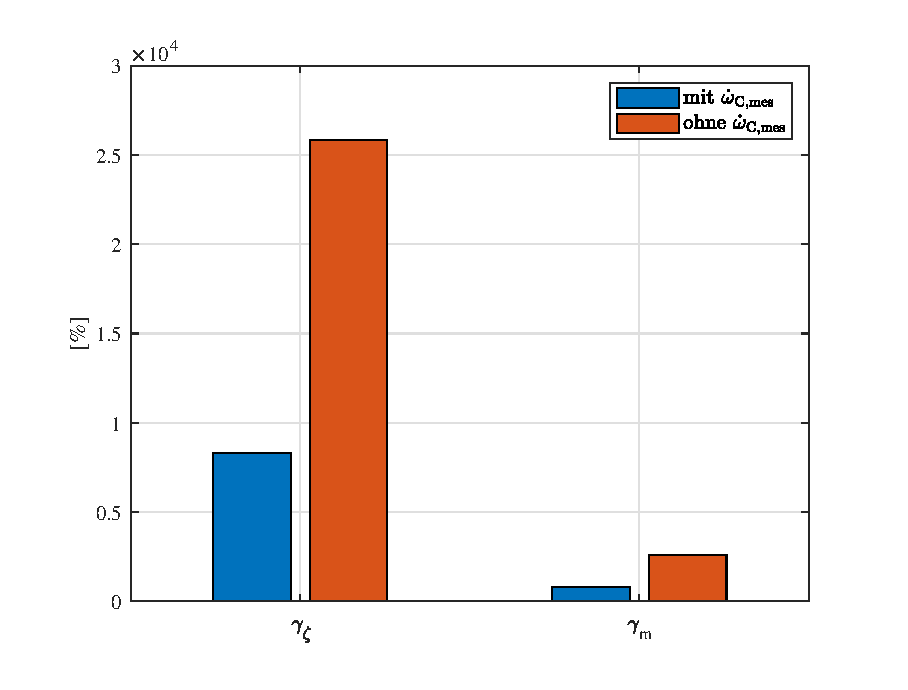
\includegraphics[scale=0.9]{figures/03_Sensitivitaetsanalyse/03_Fisher_Info/Gang2/m_vs_zeta.eps}
  \caption{Streuungen aus Fisher-Informationsmatrix für die simultane Schätzung von $m$ und $\zeta$ im 2. Gang mit $\dot{\omega}_\mathrm{C,mes}$ als Messgröße und ohne.} \label{fig:Gang2_m_z_sim}
\end{figure} 

\begin{figure}[ht]
  \centering
 \includegraphics[scale=0.9]{figures/03_Sensitivitaetsanalyse/03_Fisher_Info/Gang2/m_vs_zeta_einzeln.eps}
  \caption{Streuungen aus Fisher-Informationsmatrix für die einzelne Schätzung von $m$ und $\zeta$ im 2. Gang mit $\dot{\omega}_\mathrm{C,mes}$ als Messgröße und ohne.}\label{fig:Gang2_m_z_sep}
\end{figure} 

\subsection{Berechnung der Fisher-Informationsmatrix während der Momentenübergabe $(6\, s\leq\, t<6,5\, s )$}\label{ssec:FIMÜ}

Während der Momentenübergabe befindet sich $K_{38}$ und $B_{05}$ im Gleitbereich. Somit können die Sensitivitäten zu $\mu_{38}$ und $\mu_{05}$ nun auch mit berücksichtigt werden.
In Abbildung \ref{fig:MÜ_m_mu38_mue05_zeta} sind die Beträge der Streuungen $\gamma_{m_\mathrm{C}}$, $\gamma_{\mu_{38}}$, $\gamma_{\mu_{05}}$ und $\gamma_{\zeta}$  und  veranschaulicht. Hier liegen vor allem die Streuungen $\gamma_{\zeta}$  und $\gamma_\mathrm{m}$ ohne die Messung von $\dot{\omega}_\mathrm{C}$ sehr hoch. Jedoch deutlich derer im 2. Gang. Dies hat den Grund, dass nun eine Änderung der Beschleunigung vorliegt. Während der Einfluss von $\zeta$ beschleunigungsunabhängig ist, wirkt sich die Trägheit von $m_\mathrm{C}$ maßgeblich auf die Beschleunigung aus. Somit sind die Sensitivitätsverläufe der Messgrößen zu $m_\mathrm{C}$ und $\zeta$ nun unterschiedlich. Eine deutlich geringer Streuung ergibt sich unter der Berücksichtigung von $\dot{\omega}_\mathrm{C}$. Trotzdem liegt auch hier $\gamma_{\zeta}$ für eine praktische Anwendung noch zu hoch. Daher macht es Sinn, die Schätzung während der Momentenübergabe auf die Kombination von $m_\mathrm{C}$, $\mu_{38}$ und $\mu_{05}$ oder $\zeta$, $\mu_{38}$ und $\mu_{38}$ zu beschränken. Die sich daraus ergebenden Streuungen können Abbildung \ref{fig:MÜ_m_mu_sim} und \ref{fig:MÜ_z_mu_sim} entnommen werden. Wie in \ref{ssec:FI2Gang} führt auch hier eine separate Schätzung von $m_\mathrm{C}$ und $\zeta$ zu deutlich kleineren Streuungen. Diese liegen nun für beide Parameterkombinationen auch ohne der Berücksichtigung von $\dot{\omega}_\mathrm{C}$ unter der Grenzstreuung $\gamma_\mathrm{G}$.

\begin{figure}[ht]
  \centering
 \includegraphics[scale=0.9]{figures/03_Sensitivitaetsanalyse/03_Fisher_Info/Muebergabe/m_mu38_mue05_zeta.eps}
  \caption{Streuungen aus Fisher-Informationsmatrix für die simultane Schätzung von $m$, $\mu_{38}$, $\mu_{38}$ und $\zeta$ während der Momentenübergabe mit $\dot{\omega}_\mathrm{C,mes}$ als Messgröße und ohne.}\label{fig:MÜ_m_mu38_mue05_zeta}
\end{figure} 

\begin{figure}[ht]
  \centering
 \includegraphics[scale=0.9]{figures/03_Sensitivitaetsanalyse/03_Fisher_Info/Muebergabe/m_mu38_mue05.eps}
  \caption{Streuungen aus Fisher-Informationsmatrix für die simultane Schätzung von $m$, $\mu_{38}$ und $\mu_{05}$ während der Momentenübergabe mit $\dot{\omega}_\mathrm{C,mes}$ als Messgröße und ohne.}\label{fig:MÜ_m_mu_sim}
\end{figure} 

\begin{figure}[ht]
  \centering
 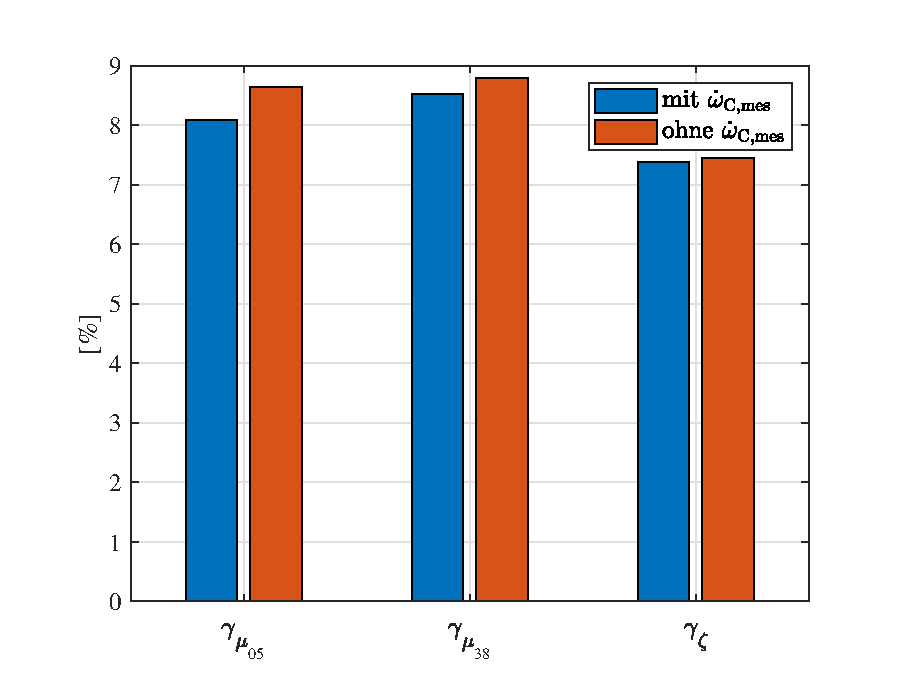
\includegraphics[scale=0.9]{figures/03_Sensitivitaetsanalyse/03_Fisher_Info/Muebergabe/mu38_mue05_zeta.eps}
  \caption{Streuungen aus Fisher-Informationsmatrix für die simultane Schätzung von $\mu_{38}$, $\mu_{05}$ und $\zeta$ während der Momentenübergabe mit $\dot{\omega}_\mathrm{C,mes}$ als Messgröße und ohne.}\label{fig:MÜ_z_mu_sim}
\end{figure} 

\subsection{Berechnung der Fisher-Informationsmatrix während der Synchronisation $(6,5\, s\leq\, t<7,0\, s )$}
Während der Synchronisation ist die Kupplung $K_{38}$ geöffnet. Der Parameter $\mu_{38}$ hat somit keinen Einfluss mehr auf die Zustände und wird daher in dieser Phase vernachlässigt. Die Beträge der Streuungen $\gamma_{m_\mathrm{C}}$, $\gamma_{\mu_{05}}$ und $\gamma_{\zeta}$ sind in Abbildung \ref{fig:m_mue05_zeta_Sync} dargestellt. Wie in \ref{ssec:FI2Gang} und \ref{ssec:FIMÜ} liegen auch hier die Werte von $\gamma_{m_\mathrm{C}}$ und $\gamma_{\zeta}$ für eine simultane Schätzung sehr hoch. Jedoch können die Streuungen mit Hilfe der Messung von $\dot{\omega}_\mathrm{C}$ wieder signifikant  gesenkt werden. In diesem Fall wären alle Streuungen schon kleiner als $\gamma_\mathrm{G}$. Werden $m_\mathrm{C}$ und $\zeta$ separat geschätzt können die Streuungen, wie in \ref{fig:m_mue05_Sync} und \ref{fig:mue05_zeta_Sync} veranschaulicht, noch weiter gesenkt werden. Hier hat vor allem die Berücksichtigung von $\dot{\omega}_\mathrm{C}$ einen positiven Einfluss auf $\gamma_{m_\mathrm{C}}$.

\begin{figure}[ht]
  \centering
 \includegraphics[scale=0.9]{figures/03_Sensitivitaetsanalyse/03_Fisher_Info/Sync/m_mue05_zeta_Sync.eps}
  \caption{Streuungen aus Fisher-Informationsmatrix für die simultane Schätzung von $m$, $\mu_{05}$ und $\zeta$ während der Synchronisation mit $\dot{\omega}_\mathrm{C,mes}$ als Messgröße und ohne.}\label{fig:m_mue05_zeta_Sync}
\end{figure} 

\begin{figure}[ht]
  \centering
 \includegraphics[scale=0.9]{figures/03_Sensitivitaetsanalyse/03_Fisher_Info/Sync/m_mue05_Sync.eps}
  \caption{Streuungen aus Fisher-Informationsmatrix für die simultane Schätzung von $m$ und $\mu_{05}$ während der Synchronisation mit $\dot{\omega}_\mathrm{C,mes}$ als Messgröße und ohne.}
  \label{fig:m_mue05_Sync}
\end{figure}

\begin{figure}[ht]
  \centering
 \includegraphics[scale=0.9]{figures/03_Sensitivitaetsanalyse/03_Fisher_Info/Sync/mue05_zeta_Sync.eps}
  \caption{Streuungen aus Fisher-Informationsmatrix für die simultane Schätzung von $\mu_{05}$ und $\zeta$ während der Synchronisation mit $\dot{\omega}_\mathrm{C,mes}$ als Messgröße und ohne.}
  \label{fig:mue05_zeta_Sync}
\end{figure}